% =====================================================================
%  Fondamenti di Unreal Engine, lezione 8 — Game Instance, livelli e
%  animazioni.
%  Ottava lezione del corso breve di introduzione a Unreal Engine
%  (focus sui Blueprint), online su Zoom, nel tardo pomeriggio (pausa
%  annunciata verso le 17:26, ripresa "55, 18", chiusura verso le 19;
%  "ci vediamo giovedì"). Docente titolare (come nelle lezioni
%  precedenti, nella trascrizione non viene mai chiamato per nome); la
%  webcam del docente non funziona per tutta la lezione, che si svolge
%  "con uno schermo nero" e lo schermo condiviso.
%  Contenuti, nell'ordine della lezione: i problemi di inizio lezione
%  (l'errore sull'Audio Component della piattaforma, rimandato alla
%  pausa); Mixamo e le Game Jam; il programma (animazioni e Gameplay
%  Framework); le variabili globali; la dimostrazione dei collezionabili
%  e della porta verso un nuovo livello; il Gameplay Framework di Unreal
%  (Game Instance, Game Mode, Game State e Player State, client e
%  server, Pawn, Character e Character Movement, Skeletal Mesh e
%  Skeleton, Animation Blueprint, Control Rig, animation programmer,
%  Player Controller, input ed Enhanced Input); il fix dell'ascensore
%  con la booleana Activated; la Game Instance GI_Platform, la variabile
%  Collectables e il Game Instance Class nei Project Settings;
%  BP_Collectible (Sphere, Sphere Collision, la doppia collisione, Get
%  Game Instance, Cast To, Increment Int, Destroy Actor); il tasto E nel
%  ThirdPersonCharacter; il volume BP_VolumeShop che azzera il conteggio
%  (Text Render, Hidden in Game) e il problema della classe genitore
%  sbagliata; il volume BP_VolumeLoadLevel con Open Level (by Name), la
%  cartella Maps, File > New Level > Basic, M_Level2 e il nome
%  case-sensitive; la prova fra i due livelli; Mixamo e la scelta del
%  personaggio in T-pose; la pausa e i problemi degli studenti; l'import
%  dell'FBX (Offset Translation e Rotation, il crash per la memoria
%  video); gli asset creati (Skeletal Mesh, Skeleton, Physics Asset,
%  materiali, l'animazione in T-pose da cancellare); lo Skeleton Editor
%  (bones e giunture: le ossa si ruotano, non si spostano); le
%  animazioni di Mixamo (overdrive, character arm space, trim, mirror,
%  root motion e in place, le impostazioni di download); l'import delle
%  animazioni sullo scheletro; l'Animation Editor (Loop, Rate Scale,
%  Root Motion); l'Animation Blueprint ABP_Knight; il nuovo Character
%  BP_Knight1 e l'Anim Class; Event Blueprint Initialize Animation, Try
%  Get Pawn Owner, il cast e le variabili di referenza; Event Blueprint
%  Update Animation, il Validated Get, Vector Length XY, GroundSpeed,
%  IsFalling e Velocity; l'AnimGraph con l'Output Pose; un'anteprima
%  del Blend Space 1D e del personaggio finito; i materiali mancanti di
%  un personaggio di Mixamo; la chiusura.
%  Fonte: trascrizione automatica dell'ottava lezione (UE8), circa tre
%  ore. Integrazioni dai libri "Blueprints Visual Scripting for Unreal
%  Engine 5" (Romero, Sewell; capitoli 3, 4 e 17) e "Blueprints Visual
%  Scripting for Unreal Engine", seconda edizione (stessi autori,
%  Unreal Engine 4), e nozioni tecniche generali su Unreal Engine 5,
%  sempre segnalate come approfondimenti.
%
%  Pacchetti richiesti nel preambolo del libro (già presenti nel
%  main.tex): \usepackage{booktabs}, \usepackage{amsmath},
%  \usepackage{amssymb}, \usepackage{tikz} con
%    \usetikzlibrary{shapes.geometric,shapes.symbols,shapes.misc,
%      arrows.meta,positioning,calc,fit}
%  (le librerie vanno caricate nel preambolo, non nel capitolo).
%  Consigliati, come per gli altri capitoli: \usepackage[italian]{babel}
%  e \usepackage[T1]{fontenc} (il capitolo compila anche senza).
%
%  Collocazione nel libro: parte "Fondamenti di Unreal Engine", ottavo
%  capitolo (numerazione propria 1.8). Nel file principale del libro,
%  subito dopo la riga della settima lezione:
%
%    % =====================================================================
%  Fondamenti di Unreal Engine, lezione 8 — Game Instance, livelli e
%  animazioni.
%  Ottava lezione del corso breve di introduzione a Unreal Engine
%  (focus sui Blueprint), online su Zoom, nel tardo pomeriggio (pausa
%  annunciata verso le 17:26, ripresa "55, 18", chiusura verso le 19;
%  "ci vediamo giovedì"). Docente titolare (come nelle lezioni
%  precedenti, nella trascrizione non viene mai chiamato per nome); la
%  webcam del docente non funziona per tutta la lezione, che si svolge
%  "con uno schermo nero" e lo schermo condiviso.
%  Contenuti, nell'ordine della lezione: i problemi di inizio lezione
%  (l'errore sull'Audio Component della piattaforma, rimandato alla
%  pausa); Mixamo e le Game Jam; il programma (animazioni e Gameplay
%  Framework); le variabili globali; la dimostrazione dei collezionabili
%  e della porta verso un nuovo livello; il Gameplay Framework di Unreal
%  (Game Instance, Game Mode, Game State e Player State, client e
%  server, Pawn, Character e Character Movement, Skeletal Mesh e
%  Skeleton, Animation Blueprint, Control Rig, animation programmer,
%  Player Controller, input ed Enhanced Input); il fix dell'ascensore
%  con la booleana Activated; la Game Instance GI_Platform, la variabile
%  Collectables e il Game Instance Class nei Project Settings;
%  BP_Collectible (Sphere, Sphere Collision, la doppia collisione, Get
%  Game Instance, Cast To, Increment Int, Destroy Actor); il tasto E nel
%  ThirdPersonCharacter; il volume BP_VolumeShop che azzera il conteggio
%  (Text Render, Hidden in Game) e il problema della classe genitore
%  sbagliata; il volume BP_VolumeLoadLevel con Open Level (by Name), la
%  cartella Maps, File > New Level > Basic, M_Level2 e il nome
%  case-sensitive; la prova fra i due livelli; Mixamo e la scelta del
%  personaggio in T-pose; la pausa e i problemi degli studenti; l'import
%  dell'FBX (Offset Translation e Rotation, il crash per la memoria
%  video); gli asset creati (Skeletal Mesh, Skeleton, Physics Asset,
%  materiali, l'animazione in T-pose da cancellare); lo Skeleton Editor
%  (bones e giunture: le ossa si ruotano, non si spostano); le
%  animazioni di Mixamo (overdrive, character arm space, trim, mirror,
%  root motion e in place, le impostazioni di download); l'import delle
%  animazioni sullo scheletro; l'Animation Editor (Loop, Rate Scale,
%  Root Motion); l'Animation Blueprint ABP_Knight; il nuovo Character
%  BP_Knight1 e l'Anim Class; Event Blueprint Initialize Animation, Try
%  Get Pawn Owner, il cast e le variabili di referenza; Event Blueprint
%  Update Animation, il Validated Get, Vector Length XY, GroundSpeed,
%  IsFalling e Velocity; l'AnimGraph con l'Output Pose; un'anteprima
%  del Blend Space 1D e del personaggio finito; i materiali mancanti di
%  un personaggio di Mixamo; la chiusura.
%  Fonte: trascrizione automatica dell'ottava lezione (UE8), circa tre
%  ore. Integrazioni dai libri "Blueprints Visual Scripting for Unreal
%  Engine 5" (Romero, Sewell; capitoli 3, 4 e 17) e "Blueprints Visual
%  Scripting for Unreal Engine", seconda edizione (stessi autori,
%  Unreal Engine 4), e nozioni tecniche generali su Unreal Engine 5,
%  sempre segnalate come approfondimenti.
%
%  Pacchetti richiesti nel preambolo del libro (già presenti nel
%  main.tex): \usepackage{booktabs}, \usepackage{amsmath},
%  \usepackage{amssymb}, \usepackage{tikz} con
%    \usetikzlibrary{shapes.geometric,shapes.symbols,shapes.misc,
%      arrows.meta,positioning,calc,fit}
%  (le librerie vanno caricate nel preambolo, non nel capitolo).
%  Consigliati, come per gli altri capitoli: \usepackage[italian]{babel}
%  e \usepackage[T1]{fontenc} (il capitolo compila anche senza).
%
%  Collocazione nel libro: parte "Fondamenti di Unreal Engine", ottavo
%  capitolo (numerazione propria 1.8). Nel file principale del libro,
%  subito dopo la riga della settima lezione:
%
%    % =====================================================================
%  Fondamenti di Unreal Engine, lezione 8 — Game Instance, livelli e
%  animazioni.
%  Ottava lezione del corso breve di introduzione a Unreal Engine
%  (focus sui Blueprint), online su Zoom, nel tardo pomeriggio (pausa
%  annunciata verso le 17:26, ripresa "55, 18", chiusura verso le 19;
%  "ci vediamo giovedì"). Docente titolare (come nelle lezioni
%  precedenti, nella trascrizione non viene mai chiamato per nome); la
%  webcam del docente non funziona per tutta la lezione, che si svolge
%  "con uno schermo nero" e lo schermo condiviso.
%  Contenuti, nell'ordine della lezione: i problemi di inizio lezione
%  (l'errore sull'Audio Component della piattaforma, rimandato alla
%  pausa); Mixamo e le Game Jam; il programma (animazioni e Gameplay
%  Framework); le variabili globali; la dimostrazione dei collezionabili
%  e della porta verso un nuovo livello; il Gameplay Framework di Unreal
%  (Game Instance, Game Mode, Game State e Player State, client e
%  server, Pawn, Character e Character Movement, Skeletal Mesh e
%  Skeleton, Animation Blueprint, Control Rig, animation programmer,
%  Player Controller, input ed Enhanced Input); il fix dell'ascensore
%  con la booleana Activated; la Game Instance GI_Platform, la variabile
%  Collectables e il Game Instance Class nei Project Settings;
%  BP_Collectible (Sphere, Sphere Collision, la doppia collisione, Get
%  Game Instance, Cast To, Increment Int, Destroy Actor); il tasto E nel
%  ThirdPersonCharacter; il volume BP_VolumeShop che azzera il conteggio
%  (Text Render, Hidden in Game) e il problema della classe genitore
%  sbagliata; il volume BP_VolumeLoadLevel con Open Level (by Name), la
%  cartella Maps, File > New Level > Basic, M_Level2 e il nome
%  case-sensitive; la prova fra i due livelli; Mixamo e la scelta del
%  personaggio in T-pose; la pausa e i problemi degli studenti; l'import
%  dell'FBX (Offset Translation e Rotation, il crash per la memoria
%  video); gli asset creati (Skeletal Mesh, Skeleton, Physics Asset,
%  materiali, l'animazione in T-pose da cancellare); lo Skeleton Editor
%  (bones e giunture: le ossa si ruotano, non si spostano); le
%  animazioni di Mixamo (overdrive, character arm space, trim, mirror,
%  root motion e in place, le impostazioni di download); l'import delle
%  animazioni sullo scheletro; l'Animation Editor (Loop, Rate Scale,
%  Root Motion); l'Animation Blueprint ABP_Knight; il nuovo Character
%  BP_Knight1 e l'Anim Class; Event Blueprint Initialize Animation, Try
%  Get Pawn Owner, il cast e le variabili di referenza; Event Blueprint
%  Update Animation, il Validated Get, Vector Length XY, GroundSpeed,
%  IsFalling e Velocity; l'AnimGraph con l'Output Pose; un'anteprima
%  del Blend Space 1D e del personaggio finito; i materiali mancanti di
%  un personaggio di Mixamo; la chiusura.
%  Fonte: trascrizione automatica dell'ottava lezione (UE8), circa tre
%  ore. Integrazioni dai libri "Blueprints Visual Scripting for Unreal
%  Engine 5" (Romero, Sewell; capitoli 3, 4 e 17) e "Blueprints Visual
%  Scripting for Unreal Engine", seconda edizione (stessi autori,
%  Unreal Engine 4), e nozioni tecniche generali su Unreal Engine 5,
%  sempre segnalate come approfondimenti.
%
%  Pacchetti richiesti nel preambolo del libro (già presenti nel
%  main.tex): \usepackage{booktabs}, \usepackage{amsmath},
%  \usepackage{amssymb}, \usepackage{tikz} con
%    \usetikzlibrary{shapes.geometric,shapes.symbols,shapes.misc,
%      arrows.meta,positioning,calc,fit}
%  (le librerie vanno caricate nel preambolo, non nel capitolo).
%  Consigliati, come per gli altri capitoli: \usepackage[italian]{babel}
%  e \usepackage[T1]{fontenc} (il capitolo compila anche senza).
%
%  Collocazione nel libro: parte "Fondamenti di Unreal Engine", ottavo
%  capitolo (numerazione propria 1.8). Nel file principale del libro,
%  subito dopo la riga della settima lezione:
%
%    % =====================================================================
%  Fondamenti di Unreal Engine, lezione 8 — Game Instance, livelli e
%  animazioni.
%  Ottava lezione del corso breve di introduzione a Unreal Engine
%  (focus sui Blueprint), online su Zoom, nel tardo pomeriggio (pausa
%  annunciata verso le 17:26, ripresa "55, 18", chiusura verso le 19;
%  "ci vediamo giovedì"). Docente titolare (come nelle lezioni
%  precedenti, nella trascrizione non viene mai chiamato per nome); la
%  webcam del docente non funziona per tutta la lezione, che si svolge
%  "con uno schermo nero" e lo schermo condiviso.
%  Contenuti, nell'ordine della lezione: i problemi di inizio lezione
%  (l'errore sull'Audio Component della piattaforma, rimandato alla
%  pausa); Mixamo e le Game Jam; il programma (animazioni e Gameplay
%  Framework); le variabili globali; la dimostrazione dei collezionabili
%  e della porta verso un nuovo livello; il Gameplay Framework di Unreal
%  (Game Instance, Game Mode, Game State e Player State, client e
%  server, Pawn, Character e Character Movement, Skeletal Mesh e
%  Skeleton, Animation Blueprint, Control Rig, animation programmer,
%  Player Controller, input ed Enhanced Input); il fix dell'ascensore
%  con la booleana Activated; la Game Instance GI_Platform, la variabile
%  Collectables e il Game Instance Class nei Project Settings;
%  BP_Collectible (Sphere, Sphere Collision, la doppia collisione, Get
%  Game Instance, Cast To, Increment Int, Destroy Actor); il tasto E nel
%  ThirdPersonCharacter; il volume BP_VolumeShop che azzera il conteggio
%  (Text Render, Hidden in Game) e il problema della classe genitore
%  sbagliata; il volume BP_VolumeLoadLevel con Open Level (by Name), la
%  cartella Maps, File > New Level > Basic, M_Level2 e il nome
%  case-sensitive; la prova fra i due livelli; Mixamo e la scelta del
%  personaggio in T-pose; la pausa e i problemi degli studenti; l'import
%  dell'FBX (Offset Translation e Rotation, il crash per la memoria
%  video); gli asset creati (Skeletal Mesh, Skeleton, Physics Asset,
%  materiali, l'animazione in T-pose da cancellare); lo Skeleton Editor
%  (bones e giunture: le ossa si ruotano, non si spostano); le
%  animazioni di Mixamo (overdrive, character arm space, trim, mirror,
%  root motion e in place, le impostazioni di download); l'import delle
%  animazioni sullo scheletro; l'Animation Editor (Loop, Rate Scale,
%  Root Motion); l'Animation Blueprint ABP_Knight; il nuovo Character
%  BP_Knight1 e l'Anim Class; Event Blueprint Initialize Animation, Try
%  Get Pawn Owner, il cast e le variabili di referenza; Event Blueprint
%  Update Animation, il Validated Get, Vector Length XY, GroundSpeed,
%  IsFalling e Velocity; l'AnimGraph con l'Output Pose; un'anteprima
%  del Blend Space 1D e del personaggio finito; i materiali mancanti di
%  un personaggio di Mixamo; la chiusura.
%  Fonte: trascrizione automatica dell'ottava lezione (UE8), circa tre
%  ore. Integrazioni dai libri "Blueprints Visual Scripting for Unreal
%  Engine 5" (Romero, Sewell; capitoli 3, 4 e 17) e "Blueprints Visual
%  Scripting for Unreal Engine", seconda edizione (stessi autori,
%  Unreal Engine 4), e nozioni tecniche generali su Unreal Engine 5,
%  sempre segnalate come approfondimenti.
%
%  Pacchetti richiesti nel preambolo del libro (già presenti nel
%  main.tex): \usepackage{booktabs}, \usepackage{amsmath},
%  \usepackage{amssymb}, \usepackage{tikz} con
%    \usetikzlibrary{shapes.geometric,shapes.symbols,shapes.misc,
%      arrows.meta,positioning,calc,fit}
%  (le librerie vanno caricate nel preambolo, non nel capitolo).
%  Consigliati, come per gli altri capitoli: \usepackage[italian]{babel}
%  e \usepackage[T1]{fontenc} (il capitolo compila anche senza).
%
%  Collocazione nel libro: parte "Fondamenti di Unreal Engine", ottavo
%  capitolo (numerazione propria 1.8). Nel file principale del libro,
%  subito dopo la riga della settima lezione:
%
%    \input{UE/UE8_game_instance_livelli_e_animazioni}
%
%  Tutte le etichette di questo capitolo hanno il prefisso "ue8:"
%  (ue8:cap:..., ue8:sec:..., ue8:fig:..., ue8:tab:...), e tutti gli
%  stili TikZ hanno il prefisso "ue8" (ue8node, ue8exec, ue8data, ...)
%  per non collidere con chiavi native di TikZ né con quelli delle
%  lezioni precedenti. Il capitolo è autonomo: non contiene \ref verso
%  altri capitoli (i rimandi alle lezioni precedenti sono a parole).
%  Le figure sono ricostruzioni schematiche di quanto mostrato e detto a
%  lezione, non copie delle slide o delle schermate del docente. Dove la
%  trascrizione è troppo rovinata per ricostruire un dettaglio, il
%  capitolo lo dice invece di inventarlo.
% =====================================================================

\chapter[Game Instance, livelli e animazioni]{Game Instance, livelli e animazioni: il
Gameplay Framework e un nuovo personaggio}
\label{ue8:cap:gameinstance}

Questa è l'\textbf{ottava lezione} del corso breve di \textbf{introduzione a Unreal
Engine}. Nelle sette lezioni precedenti tutto è avvenuto dentro un solo livello e con un
solo personaggio, il manichino del modello Third Person: la torretta, i proiettili, la
piattaforma che sale, il pulsante che attiva le luci. Oggi la lezione allarga lo sguardo
in due direzioni. La prima è \textbf{uscire dal livello}: cambiare mappa senza perdere
quello che il giocatore ha fatto, cioè \textbf{salvare dei valori in modo globale}. La
seconda è \textbf{cambiare personaggio}: prendere un modello nuovo da \textbf{Mixamo},
importarlo con il suo scheletro e le sue animazioni, e cominciare a costruire la logica
che decide quale animazione mostrare, l'\textbf{Animation Blueprint}.

Il filo che tiene insieme le due parti è il \textbf{Gameplay Framework} di Unreal: la
``gerarchia'' delle entità che l'engine crea e tiene in vita mentre il gioco gira. La
\textbf{Game Instance}, la prima a nascere e l'ultima a morire, è il posto giusto per i
dati che devono sopravvivere al cambio di livello; il \textbf{Pawn} e il
\textbf{Character}, con il loro \textbf{Character Movement}, sono la fonte dei dati
(velocità, caduta) che l'Animation Blueprint legge per animare lo scheletro. ``Andremo
sia a vedere quelle che sono le animazioni e come si gestiscono, ma sia a vedere un po'
quello che è chiamato il \emph{gameplay framework} di Unreal.''

La lezione è \textbf{online}, su Zoom, come le precedenti, ma con una particolarità: la
webcam del docente si rifiuta di funzionare per tutta la serata (``oggi mi vedrete con
uno schermo nero, o almeno il mio schermo è più importante della mia faccia''), e in
due occasioni l'editor si chiude da solo per mancanza di memoria video. Si apre con un
problema di uno studente rimandato alla pausa, prosegue con una parte teorica in slide
sul Gameplay Framework e con la costruzione dei collezionabili, della Game Instance e
dei volumi che cambiano livello; la pausa arriva verso le 17:26, con ripresa alle ``55,
18, solito orario''; la seconda parte è dedicata all'import del personaggio e delle
animazioni e all'Animation Blueprint. Il docente stesso avverte che non si arriverà in
fondo: ``probabilmente questa lezione la riporteremo nella prossima'', in cui si vedranno
i Blend Space e il resto delle animazioni. Si chiude con un ``ci vediamo giovedì''.

Tre avvertenze di lettura, le stesse delle lezioni precedenti. La prima: la
trascrizione è automatica e storpia moltissimi nomi. Unreal è ``Arena Engine'',
``Arreal'', ``a Real'', ``a RIAL'', ``Arial'' e ``Irium'' (quest'ultimo, forse, è il
programma della webcam); la \textbf{Game Instance} è ``View Instance'', ``getViewInstance''
e ``key instance''; \textbf{GI\_Platform} è ``GI Gaming Instance'', ``gi i platform'',
``asg.platform'', ``giiPatform'' e ``Di Alto''; il \textbf{Pawn} è ``Pwn'', ``la Bone'' e
``player born''; \textbf{Get Player Pawn} è ``getLayerOne'' e ``PlayerOh''; il
\textbf{Cast To} è ``castagna''; l'\textbf{On Component Begin Overlap} è ``component
baking per l'acqua'', ``onBegin onComponent onBegin overlap'' e ``On Collision Beginner
per l'app''; il \textbf{Destroy Actor} è ``destroy hardware''; il \textbf{Text Render} è
``text rendere''; la \textbf{Skeletal Mesh} è ``scheletal mesh'' e ``scheda del Mesh''; il
\textbf{Control Rig} è ``control righe''; l'\textbf{Idle} è ``Idol''; il \textbf{root
motion} è ``root in''; la \textbf{T-pose} è ``Tico'', ``tifoso'' e ``Bix ti pose'';
\textbf{FBX Binary} è ``Fibix binary''; il \textbf{Knight} è ``Night''; il \textbf{Try Get
Pawn Owner} è ``try get one''; l'\textbf{Event Blueprint Update Animation} è ``event
blueprint a data animation''; \textbf{IsFalling} è ``isPalling''; il \textbf{Diffuse} è
``Diffuse'', ma l'\textbf{eyelash} è ``ailash''; \textbf{Mixamo} è a volte
``Mixamon''. Dove la ricostruzione è sicura il capitolo usa la forma corretta; dove non
lo è riporta la forma della trascrizione e lo dice. La seconda: all'inizio della
registrazione, durante la pausa e durante i minuti lasciati per scegliere le animazioni
il riconoscimento vocale produce lunghi blocchi di testo senza senso e ripetuto
(``grazie a tutti per l'attenzione che ci ha spiegato'', ``qual è la risposta che ci può
essere?'', ``la situazione è questa, la migliore dal 2005'', ``i genitori a bordo'', la
``dottrina sul mercato del lavoro'', un Vittorio Prodi chiamato in causa senza
motivo, una lunghissima fila di ``non, non, non''): sono artefatti, non parole di nessuno,
e il capitolo li ignora. La terza: gran parte della lezione è una dimostrazione dal vivo
nell'editor, costruita a voce (``tirate fuori'', ``castate'', ``promote to variable''),
e in un paio di punti il docente improvvisa o si accorge di aver saltato un passaggio
(``ah, giusto, ragazzi, abbiamo scordato una cosa''). Il capitolo ricostruisce i grafi da
ciò che il docente dice mentre li costruisce, e li completa, dove serve, con i nomi
esatti dei nodi e dei pin di Unreal Engine 5; dove la trascrizione lascia un buco, lo
dichiara.

\paragraph{Come leggere questo capitolo.} Il capitolo segue l'ordine della lezione. Le
figure ricostruiscono la gerarchia del Gameplay Framework, la vita della Game Instance
attraverso i cambi di livello, il cast come ``abito giusto'', i grafi del collezionabile,
del tasto E e dei due volumi, la differenza fra Skeletal Mesh e Skeleton, quella fra
animazione in root motion e in place, i due grafi dell'Animation Blueprint e il Blend
Space 1D. Le tabelle riassumono le entità del framework, le impostazioni di download di
Mixamo, gli asset creati dall'import, gli errori incontrati dagli studenti e i nodi della
giornata. Qua e là, dei paragrafi di \textbf{approfondimento} collegano la lezione ai
libri di Marcos Romero e Brenden Sewell (\emph{Blueprints Visual Scripting for Unreal
Engine 5} e la seconda edizione dello stesso testo, scritta per Unreal Engine 4), i
testi di riferimento per questa parte del libro, e a qualche nozione tecnica generale su
Unreal Engine 5; sono segnalati come tali e non fanno parte della lezione.

Il percorso del capitolo:
\begin{enumerate}
  \item l'\textbf{inizio della lezione}: un errore sul suono della piattaforma, Mixamo e
        le Game Jam (sezione~\ref{ue8:sec:inizio});
  \item il \textbf{programma}, le \textbf{variabili globali} e la dimostrazione dei
        collezionabili che passano da un livello all'altro (sezioni
        \ref{ue8:sec:programma} e~\ref{ue8:sec:demo});
  \item il \textbf{Gameplay Framework} di Unreal, dalla Game Instance all'input
        (sezione~\ref{ue8:sec:framework});
  \item il \textbf{fix dell'ascensore} con la booleana Activated
        (sezione~\ref{ue8:sec:ascensore});
  \item la \textbf{Game Instance}: creazione, variabile, Project Settings
        (sezione~\ref{ue8:sec:gi});
  \item il \textbf{collezionabile}, il \textbf{cast} e il tasto E (sezioni
        da~\ref{ue8:sec:collectible} a~\ref{ue8:sec:tastoe});
  \item i due \textbf{volumi}: lo shop che azzera e il volume che \textbf{carica un
        livello} (sezioni da~\ref{ue8:sec:shop} a~\ref{ue8:sec:prova});
  \item \textbf{Mixamo}, la pausa e i problemi degli studenti (sezioni
        \ref{ue8:sec:mixamochar} e~\ref{ue8:sec:pausa});
  \item l'\textbf{import} del personaggio, lo \textbf{scheletro} e le
        \textbf{animazioni} di Mixamo (sezioni da~\ref{ue8:sec:import}
        a~\ref{ue8:sec:animeditor});
  \item l'\textbf{Animation Blueprint}, il nuovo \textbf{Character} e l'AnimGraph
        (sezioni da~\ref{ue8:sec:abp} a~\ref{ue8:sec:animgraph});
  \item i \textbf{materiali} mancanti e la chiusura (sezione~\ref{ue8:sec:chiusura}).
\end{enumerate}

% ---------------------------------------------------------------------
\section{Prima della lezione: l'Audio Component, Mixamo e le Game Jam}
\label{ue8:sec:inizio}

La registrazione comincia con i saluti (``buonasera, buonasera, buonasera'') e con le
scuse del docente: ``scusate, ragazzi, se non mi faccio vedere, ma a quanto pare ho dei
problemi con la webcam''. Il sospetto è un conflitto con OBS, il programma di
registrazione (``forse OBS potrebbe fare contrasto''); i tentativi si ripetono per tutta
la prima parte, senza successo. ``Non vi preoccupate: vi guardo, mi ascoltate, ma non mi
vedete.''

\paragraph{Le variabili chiare.} ``Come state, ragazzi? Avete un po' sperimentato?''
Uno studente ha recuperato dalla registrazione la lezione del giovedì precedente, e
racconta il suo unico problema: ``non funzionava perché nella variabile non avevo messo
il tempo, e quindi non si muoveva niente''. Il docente ne fa una regola: ``il fatto di
avere delle variabili chiare e concise ti finisce proprio il lavoro'', perché altrimenti
``stai sempre là a riguardarle'' chiedendoti ``ma perché non si muove?'', finché non ti
ricordi ``che l'hai creata di nuovo, però sta a zero''. Una variabile appena creata ha
il suo valore di default (zero, per i numeri), e un tempo, una durata o una velocità
lasciati a zero fermano tutto senza dare errori.

\paragraph{Mixamo e le Game Jam.} Uno studente chiede se il sito condiviso su Discord sia
gratuito: ``sì, sì, assolutamente, non ci avete niente da spendere''. È
\textbf{Mixamo}, ``un'ottima risorsa'' che oggi verrà usata ``in modo attivo'': essendo
uno strumento di Adobe ``abbastanza preciso nel replicare le animazioni'', e avendo
modelli ``abbastanza compatibili'' con quelli di Unreal, permette di avere personaggi e
animazioni senza animarli a mano. ``Ci sono animazioni migliori, perché esistono i pack
che si pagano fior di quattrini'', ma per cominciare Mixamo è ``il ben di Dio''. Il
docente lo usa soprattutto per le \textbf{Game Jam}: ``uno ha mai fatto una Game Jam?''
Gli studenti rispondono da soli: ``sono gli eventi dove si programma un videogioco in
pochi giorni''. ``Fondamentalmente si programma il gioco in pochi giorni, che va dai tre
giorni a una settimana'', ``poi ognuno fa un po' come gli pare''; e in quei pochi giorni,
avere animazioni pronte è ciò che fa la differenza.

\paragraph{Il primo problema: l'Audio Component che non è valido.} Filippo condivide lo
schermo. La piattaforma della lezione precedente (``quando ho fatto il bottone, l'altra
volta'') funziona, il suono si sente, ``ma poi mi dà errore'', sul \textbf{Set Pitch
Multiplier}. Il docente insegna prima un'abitudine: nel log degli errori, quando un nome
è sottolineato, ``puoi direttamente cliccare: dice proprio l'errore e ti ci porta''. Il
messaggio, in italiano, è un tentativo di accesso a un componente ``tramite la proprietà
SoundPlatform'' che ``non è valida'': ``vuol dire che l'Audio Component non è stato
spawnato o non esiste''. L'errore compare solo salendo sulla piattaforma, e solo una
volta per partita: ``lo fa solo una volta, fortunatamente'', perché ``quelle successive te
lo fa''. È, a prima vista, lo stesso caso della settima lezione (il pitch impostato prima
che il suono esista), già incontrato con un'altra studentessa.

Il docente prova un rimedio rapido: togliere i due \emph{Get} di SoundPlatform (``questi
due cilindroni'') e collegare i due Set Pitch Multiplier direttamente all'uscita del
\emph{Set} della variabile, ``così dovremmo averci la sicurezza''. Non basta: rileggendo
l'errore, il problema ``non è SoundPlatform, è l'Audio Component'' a non essere valido.
``Visto che è una cosa che ci vuole un attimino di fuori programma'', il caso viene
rimandato alla pausa (sezione~\ref{ue8:sec:pausa}): ``può essere un errore di logica di
base, poi magari sono micro cose''.

\paragraph{Approfondimento: quando l'errore compare una volta sola.} Un errore di tipo
``Accessed None'' (``accesso nullo'', ``non è valida'') che compare \emph{solo la prima
volta} è quasi sempre un problema di \textbf{ordine}: un nodo legge una variabile
referenza prima che qualcuno l'abbia riempita. Dalla seconda volta in poi la variabile
contiene il suono spawnato la volta precedente, e tutto sembra funzionare. Un errore che
compare \emph{solo arrivando in fondo} (come dirà lo studente in pausa) indica invece che
il componente esisteva ma è stato distrutto: un Sound spawnato con \textbf{Spawn Sound at
Location} ha di default l'opzione \emph{Auto Destroy} attiva, cioè l'Audio Component si
distrugge da solo quando il suono finisce o viene fermato con \textbf{Stop}, e la
variabile rimane a puntare a un oggetto non più valido. In entrambi i casi la protezione
è la stessa: un \textbf{Is Valid} prima di usare la referenza, oppure ricreare il suono
quando serve.

% ---------------------------------------------------------------------
\section{Il programma della giornata e le variabili globali}
\label{ue8:sec:programma}

``Oggi andremo a vedere un po' di particolarità.'' Il programma ha due parti:
\begin{itemize}
  \item le \textbf{animazioni}, ``e come si gestiscono'';
  \item il \textbf{Gameplay Framework} di Unreal: il fatto che l'engine, ``nella sua
        esecuzione'', ha ``una gerarchia di quello che tiene, di quello che ha'', cioè
        di entità che ``sono sempre presenti in alcuni momenti''. Fra queste c'è la
        \textbf{Game Instance}, che oggi permetterà ``di salvare dei valori in modo
        globale, chiamiamolo così''.
\end{itemize}

\paragraph{Variabile globale e variabile locale.} ``Non so se qualcuno di voi, a livello
di programmazione, sa cosa si intende con una variabile globale'' (``Federico già lo vedo
bello arzillo''). Una \textbf{variabile globale} è ``visibile in tutte le parti del
codice'': ``indipendentemente dall'ambiente in cui ci troviamo'', nel character, in un
altro oggetto, nel livello, ``è possibile visualizzarla, prenderla, modificarla''.
L'esempio opposto è a portata di mano: la variabile \textbf{ActivableItems} del pulsante
della settima lezione. ``Questa è pubblica'', con l'occhietto aperto, ``la possiamo
vedere da viewport''; ma è pubblica solo nel senso che la si modifica nei Details
dell'istanza. Esiste \emph{dentro} quel pulsante, dentro quel livello: ``se noi dovessimo
cambiare mappa, questa variabile non la potremmo più vedere'', e ``se volessimo stampare
dei valori, questo qua non esisterebbe più''. Pubblica non vuol dire globale.

\paragraph{Approfondimento: pubblica, privata, globale.} Nei Blueprint le tre parole
indicano cose diverse. Una variabile \textbf{Instance Editable} (l'occhietto) è
modificabile nei Details di ogni istanza nel livello; una variabile \textbf{Private} non
è accessibile dagli altri Blueprint, nemmeno dai child; ma in tutti i casi la variabile
\emph{vive dentro un oggetto}, e muore con lui. Quando si apre un nuovo livello, Unreal
distrugge tutti gli actor del livello precedente, compreso il personaggio del giocatore,
e ne crea di nuovi: i valori delle loro variabili tornano ai default. Unreal non ha
variabili globali nel senso dei linguaggi testuali; il modo di ottenerle è appoggiarle a
un oggetto che \emph{non} viene distrutto al cambio di livello, ed è esattamente ciò che
la lezione fa con la Game Instance (sezione~\ref{ue8:sec:gi}).

% ---------------------------------------------------------------------
\section{La dimostrazione: collezionabili e porte fra i livelli}
\label{ue8:sec:demo}

Come sempre, prima di costruire il docente mostra il risultato finito. ``Adesso vedrete
anche questo nuovo character che andremo a creare da zero, grazie all'aiuto di Mixamo'',
con ``delle animazioni nuove''; e avverte che ``cambiare character, visto che tutto
quanto va a reagire con il character'' (la piattaforma, il pulsante, i controlli sul
player), richiederà ``un piccolo fix da fare''. Per la dimostrazione, quindi, rimette il
vecchio \textbf{ThirdPersonCharacter}.

\paragraph{I collezionabili.} Nel livello ci sono delle palline: ``questi sono dei
\emph{collectable}, sono delle palline che ho creato''. Il personaggio ci passa sopra,
``1, 2, 3'', e le palline spariscono; premendo il tasto \textbf{E}, sullo schermo
compare il numero di collezionabili presi: 3.

\paragraph{La porta e il nuovo livello.} ``Oggi creeremo anche questa, che è la
porticina, che ci porterà a un nuovo livello.'' Il personaggio la attraversa e si trova
in un livello quasi vuoto. Premendo E, il conteggio è ancora 3: ``interagendo con la Game
Instance, che è sempre presente indipendentemente se io cambio livello o meno, mi posso
trasportare dei valori''. Nel secondo livello ci sono altre palline: ``se prendo questa,
ne avrò 4'', poi 5 e 6; e ``se torno al mio hub, ne avrò 6''.

\paragraph{Crash Bandicoot.} ``Non so se qualcuno di voi ha giocato a Crash Bandicoot.''
I classici della serie tengono il conto dei \textbf{cristalli}, dei \textbf{frutti Wumpa}
(``frutti Pumpa'', nella trascrizione) e delle \textbf{gemme}: ``quelli sono valori che
sono sempre salvati quando tu li prendi'', che restano tali qualunque livello si
attraversi, ``quasi totalmente globali''. Senza la Game Instance, invece, ``si
perderebbe il valore'', e il conteggio ``tornerebbe sempre a zero'': ``dovresti fare
sempre 1, 2, 3, 1, 2, 3''.

\paragraph{Che cosa ancora non fa.} Tornando nel primo livello, le palline già raccolte
sono di nuovo lì: ``questo bellissimo collectible è rispawnato''. È il comportamento
normale (il livello viene ricaricato da capo), ed è anche il prossimo esercizio
annunciato: ``andremo a fare anche un esercizio del genere, in cui andremo a dire: ehi,
guarda che questo l'ho già raccolto, levalo, non me lo far riprendere''. Cioè
``salvarci globalmente lo stato delle cose''. Nella lezione di oggi l'esercizio non viene
svolto.

% ---------------------------------------------------------------------
\section{Il Gameplay Framework di Unreal}
\label{ue8:sec:framework}

\paragraph{Che cos'è un framework.} ``Qualcuno di voi sa che cosa si intende con
\emph{framework}? Ha mai usato un framework per qualsiasi cosa, per programmazione, o
semplicemente: a volte esistono i framework per la scrittura.'' Un framework è ``uno
sviluppo base di processi'', una ``scheda da seguire''. L'esempio del docente è la
narrativa: in una storia ``c'è l'inizio, c'è lo sviluppo, c'è magari il
\emph{cliffhanger}''; un horror può essere psicologico o splatter, un film d'azione
``demenziale'' o epico, e ognuno di questi generi, ``a scelta dell'autore'', può seguire
uno schema che ``lo aiuta a sviluppare un processo di creazione''. In Unreal ``esiste
praticamente questo tipo di processo'', fatto però di ``tante piccole interfacce'', o
meglio di \textbf{entità}, che ``hanno una gerarchia tra di loro''. ``Questo, ragazzi, è
il gameplay framework di Unreal.'' Il docente lo spiega su una slide con uno schema
dall'alto verso il basso, in ordine di nascita e di ``priorità''
(figura~\ref{ue8:fig:framework}).

\paragraph{La Game Instance.} ``Quando il progetto viene lanciato, cioè l'engine'', ``la
prima cosa che viene creata, o comunque che ha priorità, è la \textbf{Game Instance}.''
È un'entità ``che va a esistere sempre, in ogni caso, quando il gioco è aperto''. Subito
dopo, nello schema, viene il caricamento del \textbf{livello}.

\paragraph{La Game Mode e Gwent.} Con il livello nasce la \textbf{Game Mode}, ``un'altra
interfaccia, che in questo caso definisce gli stati di gioco, gli stati del giocatore,
oppure le \textbf{regole del gioco}''. ``Questa Game Mode esiste assieme alla mappa'',
``e di per sé nel mondo di gioco''. L'esempio è \emph{The Witcher 3} e il suo gioco di
carte, il \textbf{Gwent}: ``state giocando al gioco normale'', parlate con un NPC che vi
propone ``un round di carte'', ``e parte il gioco delle carte''. ``In quel caso la Game
Mode cambia'': ``le regole del gioco, i punteggi, le condizioni di vittoria o sconfitta
sono gestite dalla Game Mode''.

\paragraph{Game State, Player State, client e server.} Scendendo, lo schema mostra il
\textbf{Game State}, ``lo stato del gioco, quindi tutti i dati che sono presenti'', e il
\textbf{Player State}, ``lo stato del giocatore''. Servono soprattutto quando c'è un
``interscambio di dati'', come in una cooperativa o in un multigiocatore ``con un server
di mezzo''. Una seconda slide lo mostra: ``esiste il \textbf{client}'' (``avete presente
quando aprite quello che si chiama client'') e il \textbf{server}. ``Il client comunica
con un server, e va a mandare i dati ad altri giocatori con cui giocate online'': è così
che, in uno sparatutto, ``si capisce che tipo sei morto'' e che ``quel numero delle death
o delle kill aumenta'', ``perché c'è uno scambio di stati tra i nostri player''.

\paragraph{Il Pawn.} ``Abbiamo parlato di Pawn in precedenza'': il canale di collisione
\emph{Pawn}, il nodo \emph{Get Player Pawn} usato in ogni overlap. Il docente lo descrive
così: ``il Pawn non è già il character stesso, ma è l'entità'' che può essere
controllata, dal giocatore ``o addirittura dall'AI'', cioè ``o da input del giocatore,
oppure da un processo di \emph{behavior}, un comportamento già stabilito, come può essere
un nemico''. Al Pawn ``vengono date'' le componenti, la mesh, la navigazione, le
animazioni, il \emph{view target} (la camera) e, ``se ci fossero'', i \textbf{physical
material}, ``materiali che hanno delle proprietà fisiche'', da vedere più avanti.

\paragraph{Il Character e il Character Movement.} ``Il character stesso è subito dopo.''
Il Character ha ``le sue particolarità di movimento'', raccolte nel \textbf{Character
Movement Component}, con dati ``che possono essere modificati'':
\begin{itemize}
  \item le \textbf{movement mode}: ``come mi sto muovendo'', cioè se sta camminando, se
        sta volando (\emph{flying}), se sta nuotando, oppure un \emph{custom movement},
        ``un movimento particolare'', come una scivolata;
  \item le \textbf{movement capabilities}: ``quanto mi posso muovere, quanto veloce
        sono'', la \emph{braking friction}, ``cioè quanto ci metto a frenare'';
  \item le \textbf{interazioni fisiche};
  \item la \textbf{replicazione}, cioè il movimento condiviso in rete.
\end{itemize}

\paragraph{Skeletal Mesh e Skeleton.} Il Character ha anche la sua \textbf{mesh}, ``la
sua particolarità di avere la sua forma''. ``La Skeletal Mesh e lo scheletro sono due
cose completamente diverse, ragazzi.'' Lo \textbf{scheletro} è fatto di ossa, le
\textbf{bones}, ed è il prodotto del \textbf{rigging}, ``il compito di un povero ragazzo
o ragazza che si mette là a creare le ossa'', ``un lavoro a sé stante''; poi c'è
l'\textbf{animatore}, ``che ruota queste ossa per compiere un'animazione''. La
\textbf{Skeletal Mesh} ``è fondamentalmente una mesh con uno scheletro'': ``la forma più
le ossa'', ``il corpo e le ossa''. Lo scheletro è un asset separato, ``gestito in
un'altra modalità'', in cui si vedono ``tutte quante le ossa del nostro bellissimo
character'' (figura~\ref{ue8:fig:skeletal}). Le ossa si controllano con
l'\textbf{Animation Graph}, ``spesso chiamato Animation Blueprint'', che oggi verrà
creato, e con il \textbf{Control Rig}, ``una cosa che è stata messa da Unreal'' per
animare direttamente nell'editor, che però oggi ``non ci servirà''.

\paragraph{L'animation programmer.} ``Sappiate che ci sono delle figure professionali''
che non sono solo l'animatore: c'è l'\textbf{animation programmer}. ``Fate conto che sono
due fratellini'': in uno studio dove ha lavorato il docente ``andavano avanti e indietro
continuamente'', ``uno fa le animazioni, l'altro le gestisce, con la logica''. L'esempio
è il \textbf{piede sullo scalino}: in molti giochi ``i piedi vengono inclinati'' quando il
personaggio sta su un piano inclinato o su un gradino. ``Quella cosa non è fatta da un
animatore, assolutamente no'': è fatta da un animation programmer, che ``prende le ossa
della camminata'' e dà ``un set di regole'': ``guarda che, se c'è un dislivello di 20
gradi, l'osso va ruotato in questo modo e va messo sopra lo scalino'', ``la pianta del
piede va ruotata e messa in allineamento''. Sul character base di Unreal questa
particolarità ``già c'è'', ``perché ormai è una cosa strausata''.

\paragraph{Il Player Controller.} Più in basso nello schema c'è il \textbf{Player
Controller}. ``Se dovessimo andare per una meccanica'' in cui modificare ``i parametri di
controllo'', per esempio ``switchare tra character'' (``controllo uno, controllo
l'altro''), si lavora con il controller, che ``è un'entità a sé stante''. I controller
``sono actor non fisici'': ``non li potete vedere''.

\paragraph{L'input.} ``L'ultima cosa, che veramente è in fondo, è che quasi qua ci siamo
noi'': l'\textbf{input}, ``la forma più esterna di interazione tra la macchina e noi'', da
cui parte ``tutto quanto il percorso del gameplay framework''. Esiste un sistema
moderno, l'\textbf{Enhanced Input System}, ``molto interessante'', ``che ci permette di
destreggiarci negli input'': per ora non verrà usato (``andremo a vedere forme molto più
blande''), ma più avanti forse si creerà ``un sistema di input interfacciato con Enhanced
Input''. ``Tutto questo ambaradam è come Unreal capisce e comprende'' il gioco, e gli dà
``una gerarchia''. ``Visto che vi ho riempito di chiacchiere, andiamo a vedere con la
ciccia, con la pratica.''

\begin{figure}[htbp]
\centering
\begin{tikzpicture}[font=\footnotesize,
  ue8fw/.style={draw, thick, rounded corners=4pt, align=center, minimum height=0.85cm,
                text width=3.0cm},
  ue8note/.style={font=\scriptsize, align=left, text width=6.6cm, anchor=west},
  ue8arr/.style={-{Stealth[length=2.2mm]}, thick, black!70}]
  \node[ue8fw, fill=green!18] (eng) at (0,0) {\textbf{Engine}\\(avvio del gioco)};
  \node[ue8fw, fill=green!30] (gi) at (0,-1.3) {\textbf{Game Instance}};
  \node[ue8fw, fill=gray!12] (lv) at (0,-2.6) {\textbf{Livello} (World)};
  \node[ue8fw, fill=orange!22] (gm) at (0,-3.9) {\textbf{Game Mode}};
  \node[ue8fw, fill=orange!12] (gs) at (0,-5.2) {\textbf{Game State} /\\ \textbf{Player
    State}};
  \node[ue8fw, fill=blue!12] (pc) at (0,-6.6) {\textbf{Player Controller}};
  \node[ue8fw, fill=blue!20] (pw) at (0,-8.15) {\textbf{Pawn} $\rightarrow$
    \textbf{Character}\\(Character Movement, Skeletal Mesh, Anim BP)};
  \node[ue8fw, fill=red!12] (in) at (0,-9.95) {\textbf{Input}\\(noi)};
  \foreach \a/\b in {eng/gi, gi/lv, lv/gm, gm/gs, gs/pc, pc/pw} \draw[ue8arr] (\a) -- (\b);
  \draw[ue8arr] (in) -- (pw);
  \node[ue8note] at (2.0,-1.3) {la prima a nascere, l'ultima a morire: sopravvive al
    cambio di livello (``i dati globali'')};
  \node[ue8note] at (2.0,-2.6) {quando si apre un livello, tutti i suoi actor vengono
    creati da capo};
  \node[ue8note] at (2.0,-3.9) {le regole: punteggi, vittoria, sconfitta (il Gwent
    cambia la Game Mode); una per livello};
  \node[ue8note] at (2.0,-5.2) {lo stato della partita e di ogni giocatore; condivisi
    fra client e server in multigiocatore};
  \node[ue8note] at (2.0,-6.6) {il ``cervello'' non fisico: possiede un Pawn, e può
    cambiarlo};
  \node[ue8note] at (2.0,-8.15) {il ``corpo'' nel mondo; il Character è il Pawn che
    cammina, salta, nuota, vola};
  \node[ue8note] at (2.0,-9.95) {tastiera, mouse, gamepad; in futuro l'Enhanced Input
    System};
  \draw[very thick, green!40!black] (-1.75,-0.9) -- (-1.75,-1.7);
  \node[left, font=\scriptsize, align=right, text=green!40!black] at (-1.8,-1.3)
    {tutta la\\durata\\del gioco};
  \draw[very thick, orange!50!black] (-1.75,-2.2) -- (-1.75,-8.8);
  \node[left, font=\scriptsize, align=right, text=orange!50!black] at (-1.8,-5.5)
    {ricreati\\a ogni\\livello};
\end{tikzpicture}
\caption{Il Gameplay Framework come lo presenta il docente: dall'alto verso il basso, in
ordine di nascita e di ``priorità''. La Game Instance esiste per tutta la durata del
gioco; tutto quello che sta sotto il livello viene distrutto e ricreato a ogni cambio di
mappa. Schema ricostruito; le note a destra riassumono la spiegazione.}
\label{ue8:fig:framework}
\end{figure}

\paragraph{Approfondimento: chi possiede chi.} Nella spiegazione a voce i ruoli di Pawn
e Controller si confondono un po' (``il Pawn è l'entità che lo possiede''). Romero e
Sewell (capitolo 3, ``Object-Oriented Programming and the Gameplay Framework'') li
distinguono con un'immagine netta: il \textbf{Pawn} è ``il corpo fisico'' del
personaggio, un actor che può essere \emph{posseduto}; il \textbf{Controller} che lo
possiede è ``una specie di cervello'', e rappresenta un giocatore umano
(\textbf{PlayerController}) o un'intelligenza artificiale (\textbf{AIController}). Il
nodo \textbf{Possess} permette al controller di cambiare corpo, ed è il meccanismo del
``controllo uno, controllo l'altro'' del docente: nel loro esempio due Character nel
livello si alternano premendo 1 o 2, e riceve i comandi solo quello posseduto. Il
\textbf{Character} è un figlio del Pawn pensato per personaggi ``che camminano, corrono,
saltano, nuotano e volano'', ed eredita quattro componenti: \emph{CapsuleComponent} (le
collisioni), \emph{ArrowComponent} (la direzione), \emph{Mesh} (una Skeletal Mesh,
animata da un Animation Blueprint) e \emph{CharacterMovement}, che gestisce anche
``replicazione e predizione nei giochi multigiocatore''. Per ereditarietà, un Character è
anche un Pawn e anche un Actor: è per questo che il confronto con \emph{Get Player Pawn}
funziona su un Character.

\paragraph{Approfondimento: la Game Mode del livello.} Sempre nel capitolo 3, gli autori
precisano che la \textbf{Game Mode} non definisce solo le regole, ma anche le
\emph{classi di default} usate dal gioco: il Pawn che il giocatore riceve
(\emph{Default Pawn Class}), il PlayerController, il Game State, l'HUD. Si imposta per
tutto il progetto in \emph{Project Settings $\rightarrow$ Maps \& Modes $\rightarrow$
Default GameMode}, e si può sostituire livello per livello in \emph{World Settings
$\rightarrow$ GameMode Override}. È proprio lì, nei World Settings, che a fine lezione il
docente cambierà il personaggio del giocatore (sezione~\ref{ue8:sec:animgraph}). La
\textbf{Game Instance}, invece, ``non è una delle classi comuni'', ma ``è importante
sapere che esiste'': viene creata all'inizio del gioco ed eliminata solo quando il gioco
si chiude, mentre ``tutti gli actor e gli altri oggetti di un livello vengono distrutti e
ricreati ogni volta che un livello viene caricato''. Per questo è ``un'opzione da usare
se si devono conservare dei valori nella transizione fra livelli''.

\begin{table}[htbp]
\centering
\small
\begin{tabular}{@{}p{3.0cm}p{5.6cm}p{5.4cm}@{}}
\toprule
\textbf{Entità} & \textbf{Che cosa fa} & \textbf{Esempio della lezione} \\
\midrule
Game Instance & esiste dall'avvio alla chiusura del gioco; conserva i dati fra i
livelli & il conteggio dei collezionabili; il personaggio scelto \\
Game Mode & le regole: punteggi, condizioni di vittoria e sconfitta, classi di default;
nasce con il livello & il Gwent di \emph{The Witcher 3} \\
Game State & lo stato della partita, condiviso fra i giocatori & i dati di una
cooperativa con un server \\
Player State & lo stato di un singolo giocatore & le kill e le death in uno sparatutto
online \\
Pawn & l'actor che può essere controllato, dal giocatore o da un'AI & Get Player Pawn
nei controlli di overlap \\
Character & il Pawn con capsula, Skeletal Mesh e Character Movement & il
ThirdPersonCharacter, il nuovo BP\_Knight1 \\
Character Movement & movement mode, velocità, frenata, fisica, replicazione & la
velocità letta dall'Animation Blueprint \\
Player Controller & entità non fisica che riceve l'input e possiede il Pawn & passare
da un personaggio all'altro \\
Input & tasti, mouse, gamepad; Enhanced Input System & il tasto E che stampa il
conteggio \\
\bottomrule
\end{tabular}
\caption{Le entità del Gameplay Framework presentate a lezione. Le precisazioni su Game
Mode e Controller seguono Romero e Sewell (capitolo 3).}
\label{ue8:tab:framework}
\end{table}

% ---------------------------------------------------------------------
\section{Un fix per l'ascensore: la booleana Activated}
\label{ue8:sec:ascensore}

Il docente apre il progetto (``mi sono scordato'') e invita a creare una cartella nuova
(``tasto destro, solita cosa''), ma prima di cominciare si ferma: ``ah, ragazzi,
aspettate, mi sono ricordato di una cosa che volevo farvi fare''. È ``un piccolo fix per
l'\textbf{ascensore} col pulsante'', cioè la piattaforma attivabile del compito della
settima lezione: la piattaforma che, comandata dal pulsante, scende, e che risale quando
il giocatore ci sale sopra. ``Il problema era che si bloccava'': ``andava sempre più giù
e non si muoveva più''.

\paragraph{La cura.} ``Basta mettere una booleana.'' Nella piattaforma si crea una
variabile booleana, \textbf{Activated}, e la si usa come un cartello ``già fatto'':
\begin{itemize}
  \item all'inizio dell'evento \textbf{Activation} si mette un \textbf{Branch} con
        Activated come condizione; dall'uscita \textbf{False} si fa \textbf{Set
        Activated} a \emph{true} e poi si prosegue con la logica che c'era (il Play
        della timeline). Dall'uscita True non parte niente: se la piattaforma è già
        attivata, una seconda attivazione viene ignorata;
  \item sull'\textbf{On Component Begin Overlap} della box (il player che sale e fa
        risalire la piattaforma) si rimette Activated a \emph{false}, in modo che la
        prossima pressione del pulsante possa di nuovo farla scendere.
\end{itemize}
``Questo dovrebbe risolvere il fatto che l'ascensore vada continuamente giù''
(figura~\ref{ue8:fig:ascensore}). Nella trascrizione la frase esatta è confusa
(``deve essere un branch con il false, mettete activated come condizione principale'');
la struttura qui sopra è quella che il docente rifarà passo per passo con uno studente
in pausa (sezione~\ref{ue8:sec:pausa}).

\begin{figure}[htbp]
\centering
\begin{tikzpicture}[font=\footnotesize,
  ue8node/.style={draw, thick, rounded corners=4pt, align=center, fill=gray!8,
                  minimum height=0.8cm, text width=2.1cm},
  ue8ev/.style={ue8node, fill=red!12},
  ue8var/.style={ue8node, fill=red!6, rounded corners=8pt, text width=1.7cm},
  ue8exec/.style={-{Stealth[length=2.5mm]}, very thick, black!80},
  ue8data/.style={-{Stealth[length=2mm]}, thick, red!60!black}]
  % Activation
  \node[ue8ev] (act) at (0,0) {\textbf{Event}\\Activation};
  \node[ue8node] (br) at (3.2,0) {\textbf{Branch}};
  \node[ue8var] (get) at (3.2,-1.5) {Activated};
  \node[ue8node] (set1) at (6.6,0) {\textbf{Set Activated}\\= true};
  \node[ue8node, fill=red!8] (play) at (9.8,0) {Timeline\\\textbf{Play}};
  \node[font=\scriptsize, text=gray!70!black, align=left, anchor=west] at (4.4,-1.2)
    {True: già attivata,\\non succede niente};
  \draw[ue8exec] (act) -- (br);
  \draw[ue8data] (get) -- node[right, font=\scriptsize]{Condition} (br);
  \draw[ue8exec] (br) -- node[above, font=\scriptsize]{False} (set1);
  \draw[ue8exec] (set1) -- (play);
  % Begin overlap
  \node[ue8ev, text width=2.6cm] (ov) at (0,-3.4) {\textbf{On Component Begin
    Overlap}\\(Box)};
  \node[ue8node, text width=2.4cm] (chk) at (3.4,-3.4) {Other Actor ==\\Get Player
    Pawn $\rightarrow$ \textbf{Branch}};
  \node[ue8node] (set2) at (6.6,-3.4) {\textbf{Set Activated}\\= false};
  \node[ue8node, fill=red!8] (rev) at (9.8,-3.4) {Timeline\\\textbf{Reverse}};
  \draw[ue8exec] (ov) -- (chk);
  \draw[ue8exec] (chk) -- node[above, font=\scriptsize]{True} (set2);
  \draw[ue8exec] (set2) -- (rev);
\end{tikzpicture}
\caption{Il fix dell'ascensore. La booleana Activated impedisce che una seconda
attivazione rimandi giù la piattaforma già scesa; quando il player ci sale sopra e la
fa risalire, Activated torna a false. Schema ricostruito.}
\label{ue8:fig:ascensore}
\end{figure}

\paragraph{Approfondimento: la booleana come cancello.} Una variabile booleana usata così
è un \emph{flag}, o un \emph{gate}: un cancello che lascia passare l'esecuzione una volta
e poi resta chiuso finché qualcun altro non lo riapre. È la versione ``a mano'' del nodo
\textbf{Do Once}, già usato nella sesta lezione per il suono, che ha un ingresso
\emph{Reset}; scritta con un Branch e una variabile ha il vantaggio di essere leggibile
da altri punti del Blueprint (per esempio da un Print String, mentre si fa debug) e di
poter essere riaperta da un evento qualsiasi. Il problema che risolve è comune a tutti
gli oggetti comandati da più eventi: un Play chiamato mentre la timeline è già alla fine
non fa nulla di visibile, ma la combinazione di Play, Reverse e Set New Time chiamati
nell'ordine sbagliato può spostare la posizione di partenza dei calcoli.

\paragraph{Una chiavetta USB.} Una studentessa segnala che il progetto non si apre:
``mi apre solo UE senza andare dentro''. Potrebbe essere ``un problema di import''; il
consiglio vale per tutti: ``attenzione con le chiavette USB, a staccarle'' sempre in modo
sicuro, ``perché se no vi fate i problemi''. ``Servirebbe un \textbf{Git}'', cioè un
sistema di controllo di versione, ``però di base fate attenzione''. E comunque ``c'è la
registrazione''.

% ---------------------------------------------------------------------
\section{La Game Instance: GI\_Platform}
\label{ue8:sec:gi}

``Allora, questo è solo un piccolo fix, ragazzi. E adesso partiamo con il nostro
bellissimo Game Instance.'' Si crea una cartella \textbf{GameInstance}, la si apre, e si
crea la Game Instance del progetto: ``sarà praticamente il \textbf{cervello principale},
che sarà possibile visualizzare da ogni parte, che cambiamo mappa o che non cambiamo
mappa''.

\paragraph{La creazione.} Si fa \textbf{Blueprint Class}, ``al solito''. Nella finestra
che chiede la classe genitore, i bottoni in alto sono le classi comuni; sotto ``potete
abbassare una tendina'' (\textbf{All Classes}), ``e sono presenti tutte le classi di tutti
gli attori che potete creare''. Si cerca \textbf{GameInstance}: ``dovreste trovare Object
$\rightarrow$ GameInstance''. Select, e il nome: \textbf{GI\_Platform}, con il prefisso
GI per ``Game Instance'' (``la chiamiamo Platform''). Aperta, ``vi si presenterà come un
normalissimo Blueprint, che abbiamo già visto tante volte ormai, ma completamente
vuoto'': ``non c'è una viewport, non c'è niente, è solo un'entità non fisica''. Dentro si
possono creare ``delle funzioni, delle macro, delle variabili, degli event dispatcher,
come abbiamo visto le altre volte''.

\paragraph{La variabile.} Si crea una variabile di tipo \textbf{Integer}, chiamata
\textbf{Collectables}. ``Da questo momento in poi questa variabile, assieme alla Game
Instance, viaggerà assieme a lei'': ``il suo valore'', che lo modifichiamo o no,
``quando sta all'interno della Game Instance rimane tale''.

\paragraph{I Project Settings.} ``Adesso dobbiamo dire al gioco quale Game Instance devi
usare. Perché lui userà la sua di default, che si trova da qualche parte nei file
dell'engine.'' Da \textbf{Edit $\rightarrow$ Project Settings} si cerca ``Game Instance'':
compare, sotto \textbf{Project $\rightarrow$ Maps \& Modes}, la voce \textbf{Game Instance
Class}. Dalla tendina si sceglie \textbf{GI\_Platform}. ``Adesso la Game Instance del
gioco, fino a che il gioco è in esecuzione, userà questa.''

\paragraph{Non appesantirla.} ``Sappiate che, quando si va in esecuzione, questa Game
Instance esiste sempre; quindi è molto importante anche \textbf{non appesantirla}.''
``Questa è perenne finché non chiudete il gioco'': ``non è fisica, ma si porta dietro la
roba''. Tutto ciò che vi si mette resta in memoria per l'intera partita.

\begin{figure}[htbp]
\centering
\begin{tikzpicture}[font=\footnotesize,
  ue8lv/.style={draw, thick, rounded corners=3pt, fill=gray!10, minimum height=1.6cm,
                text width=2.7cm, align=center},
  ue8arr/.style={-{Stealth[length=2.2mm]}, thick}]
  \fill[green!18, rounded corners=4pt] (-0.2,2.1) rectangle (12.4,2.9);
  \node[font=\small\bfseries] at (6.1,2.5) {GI\_Platform \quad Collectables = 0
    $\rightarrow$ 3 $\rightarrow$ 6 $\rightarrow$ 9};
  \node[ue8lv] (l1) at (1.6,0.5) {\textbf{ThirdPersonMap}\\3 palline raccolte};
  \node[ue8lv] (l2) at (6.1,0.5) {\textbf{M\_Level2}\\3 palline raccolte};
  \node[ue8lv] (l3) at (10.6,0.5) {\textbf{ThirdPersonMap}\\(ricaricata: le palline\\
    sono di nuovo lì)};
  \draw[ue8arr] (l1) -- node[above, font=\scriptsize, align=center]{Open\\Level} (l2);
  \draw[ue8arr] (l2) -- node[above, font=\scriptsize, align=center]{Open\\Level} (l3);
  \foreach \l in {l1, l2, l3} \draw[thick, dashed, green!40!black] (\l.north) -- ++(0,0.75);
  \node[font=\scriptsize, align=center, text width=12cm] at (6.1,-0.9) {ogni livello
    distrugge i suoi actor quando si esce; la Game Instance resta, e con lei il
    conteggio};
\end{tikzpicture}
\caption{Perché la Game Instance. I livelli si aprono e si chiudono, e a ogni apertura
gli actor (palline comprese) vengono ricreati; la Game Instance esiste sopra di loro per
tutta la durata del gioco, e la sua variabile Collectables continua a contare. Schema
ricostruito dalla dimostrazione.}
\label{ue8:fig:persistenza}
\end{figure}

\paragraph{Approfondimento: che cosa mettere nella Game Instance.} Oltre ai contatori, la
Game Instance è il posto tipico per le \emph{impostazioni} scelte nel menù (volume,
difficoltà), per il personaggio selezionato prima di entrare in partita (l'esempio che il
docente farà a fine prima parte), per lo stato della sessione online e per un
riferimento al salvataggio corrente. Ha però due limiti da ricordare. Il primo: vive
quanto il \emph{processo} del gioco, non di più; chiuso il gioco, i suoi valori sono
persi. Per conservarli su disco, Unreal usa un oggetto diverso, il \textbf{SaveGame},
con i nodi \emph{Create Save Game Object}, \emph{Save Game to Slot} e \emph{Load Game
from Slot}. Il secondo: nel Play in Editor (PIE) la Game Instance viene creata a ogni
pressione di Play, quindi ogni prova ricomincia da zero. Infine, una differenza con la
Game Mode: in un gioco in rete la Game Mode esiste solo sul server, mentre ogni client ha
la propria Game Instance; per i dati da condividere fra giocatori servono Game State e
Player State.

% ---------------------------------------------------------------------
\section{Il collezionabile: BP\_Collectible}
\label{ue8:sec:collectible}

``Adesso cosa facciamo? Dobbiamo creare quello che sarà il nostro collectable.'' Sarà
``una pallina, come vi pare''; volendo, ``possiamo anche creare il materiale''. Nella
cartella dei Blueprint (``mani con me, quando siete ordinati'') si crea una
\textbf{Blueprint Class} di tipo \textbf{Actor} (``non ci serve una roba particolare''),
chiamata \textbf{BP\_Collectible}.

\paragraph{I componenti.} Si aggiunge una mesh: ``volendo, possiamo pure senza mettere
Static Mesh'' e aggiungere direttamente il componente \textbf{Sphere} delle forme di
base, che è già una Static Mesh con la sfera assegnata. La si rinomina \textbf{Mesh}. Poi
la collisione: \textbf{Sphere Collision}, chiamata \textbf{Collision}. Le dimensioni:
\begin{itemize}
  \item la mesh si rimpicciolisce a \textbf{scala 0,5} (``facciamo un po' più
        piccolina''). ``Ricordatevi del \textbf{lucchetto}'': se il lucchetto della scala
        è aperto ``vi cambia solamente un valore''; se è chiuso, la modifica è
        \textbf{uniforme}, ``vi cambia tutti e tre i valori'';
  \item la Sphere Collision ha il suo \textbf{Sphere Radius}, ``il raggio della nostra
        sfera'', ``come abbiamo visto anche con la torretta''. Un trucco per regolarlo:
        mettere il mouse sopra il numero e trascinare a destra e a sinistra, ``fate un
        po' da slide''. Il docente arriva a circa \textbf{52} (``io ce l'ho 52, va
        benissimo'').
\end{itemize}
Per il materiale, ``ci possiamo sbizzarrire''; il docente ne prende uno fra quelli già
presenti nel progetto, \textbf{Hologrid} (``carino''). Nella trascrizione il nome della
cartella da cui lo prende è illeggibile.

\paragraph{La doppia collisione.} ``Una piccola accortezza che vi consiglio.'' La pallina
ha due collisioni: quella della Sphere Collision e quella della mesh. Il docente lo
mostra con un overlap provvisorio che distrugge l'actor: passandoci sopra, ``c'è un
momento proprio minuscolo in cui il character si ferma'', ``perché ha fatto
\textbf{doppia collisione}''. Prima di sparire, la pallina blocca il personaggio per un
frame con la sua mesh. Per i collezionabili, ``cose che voi prendete tranquillamente'', è
meglio che la mesh non abbia collisioni: sulla mesh, \textbf{Collision Presets
$\rightarrow$ NoCollision}. Due vantaggi: si alleggerisce l'asset, ``e andremo anche a
semplificare il gameplay'', perché quel micro arresto ``il player lo sente'', soprattutto
``dopo tante'' palline sparse in giro.

\paragraph{Il controllo sul player.} Selezionata la Collision, si crea l'evento
\textbf{On Component Begin Overlap}. Poi ``quello che ormai abbiamo fatto 30.000 volte'':
\textbf{Other Actor} confrontato con \textbf{Get Player Pawn} (il nodo \textbf{==}),
collegato a un \textbf{Branch}: ``sempre un controllo di norma''.

\paragraph{Il problema: dove tenere il conto.} ``Adesso che cosa dobbiamo fare? Dobbiamo
distruggere l'actor.'' Ma prima bisogna contare la pallina, e il conto non può stare
nella pallina, che sparisce, né nel personaggio, che sparisce al cambio di livello: ``visto
che questa cosa dovrà essere sempre presente, possiamo usare la Game Instance''. ``Visto
che la Game Instance è richiamabile praticamente ovunque'', basta un tasto destro e
\textbf{Get Game Instance}: ``ecco a voi che questo blocchetto ci ridà indietro la nostra
bella Game Instance''. ``Se avete delle cose molto importanti, come ad esempio il
punteggio, i tempi, i costi, i salvataggi'', ``la Game Instance è \emph{the way}''.

% ---------------------------------------------------------------------
\section{Il cast: entrare nella scocca}
\label{ue8:sec:cast}

``Perché, ad esempio, se noi tiriamo fuori'' dall'uscita di Get Game Instance ``e
facciamo Get Collectables, vedete che non appare niente.'' Il nodo restituisce una
referenza di tipo generico \emph{Game Instance}: ``ha preso una referenza, ma non ha
preso l'interno''. ``Sta sulla \textbf{scocca}, diciamolo così'': ``prende le proprietà
della Game Instance come asset a sé, ma non quello interno''. ``Quindi dobbiamo penetrare
nella scocca. Come lo facciamo? Grazie a quello che viene chiamato il \textbf{cast}'':
\textbf{Cast To GI\_Platform}.

\paragraph{Il nodo.} Il cast ``ci dice: tramite lui, vai a questo oggetto, prova a
collegarti'' a GI\_Platform. Ha:
\begin{itemize}
  \item l'ingresso \textbf{Object}, in cui va il Return Value di Get Game Instance;
  \item l'uscita di esecuzione principale, quella in alto, che corrisponde al
        \textbf{cast riuscito}: ``Cast Successful non c'è scritto, ma questo sopra ci
        dice che il collegamento tra le due è avvenuto'';
  \item l'uscita \textbf{Cast Failed}, ``il collegamento non è avvenuto, non è riuscito
        a collegarsi'';
  \item il pin blu \textbf{As GI Platform}, ``la referenza dello specifico'' oggetto,
        ``come GI Platform fai questa cosa''.
\end{itemize}

\paragraph{La festa di gala.} Più tardi uno studente chiede: ``non ho capito a cosa
servono quei due nodi, il cast''. ``Serve per mettere in comunicazione la Game Instance
con l'asset specifico'': ``come actor Game Instance, prova a entrare all'interno della
GI\_Platform''. E la metafora: ``è come dirti: mettiti un abito e prova a entrare a una
\textbf{festa di gala}''. ``Se l'abito non è giusto'', non entri; ``se invece è quello
corretto, vuol dire che puoi entrare e far parte, quindi puoi prendere tutti gli
stuzzichini che ti pare''. ``Indosso l'abito giusto per il contesto giusto''
(figura~\ref{ue8:fig:cast}).

\begin{figure}[htbp]
\centering
\begin{tikzpicture}[font=\footnotesize,
  ue8box/.style={draw, thick, rounded corners=5pt, align=center},
  ue8arr/.style={-{Stealth[length=2.2mm]}, thick}]
  % referenza generica
  \node[ue8box, fill=gray!12, minimum width=3.6cm, minimum height=2.6cm] (gen) at (0,0) {};
  \node[font=\small\bfseries] at (0,0.95) {Game Instance};
  \node[font=\scriptsize, align=center] at (0,0.2) {la ``scocca'':\\vede solo ciò
    che\\ha ogni Game Instance};
  \node[font=\scriptsize, text=red!70!black] at (0,-0.85) {Collectables? non c'è};
  % cast
  \node[ue8box, fill=blue!12, text width=2.4cm, minimum height=1.1cm] (cast) at (4.3,0)
    {\textbf{Cast To}\\\textbf{GI\_Platform}};
  \draw[ue8arr] (gen) -- node[above, font=\scriptsize]{Object} (cast);
  % specifico
  \node[ue8box, fill=green!14, minimum width=3.8cm, minimum height=2.6cm] (spec) at (9.0,0.7) {};
  \node[font=\small\bfseries] at (9.0,1.65) {As GI Platform};
  \node[font=\scriptsize, align=center] at (9.0,0.95) {``dentro la scocca'':\\l'abito
    giusto, si entra};
  \node[font=\scriptsize, text=green!40!black] at (9.0,0.0) {Collectables (Integer)};
  \node[ue8box, fill=red!10, text width=3.4cm] (fail) at (9.0,-1.6) {\textbf{Cast
    Failed}: l'abito è sbagliato};
  \draw[ue8arr] (cast.east) -- ++(0.5,0) |- (spec.west);
  \draw[ue8arr] (cast.east) -- ++(0.5,0) |- (fail.west);
\end{tikzpicture}
\caption{Il cast come lo spiega il docente. Get Game Instance restituisce una referenza
generica, che conosce solo ciò che ogni Game Instance ha; il Cast To GI\_Platform prova
a ``indossare l'abito'' della nostra classe: se l'oggetto è davvero una GI\_Platform, il
pin As GI Platform dà accesso alle sue variabili; se no, si esce da Cast Failed. Schema
ricostruito.}
\label{ue8:fig:cast}
\end{figure}

\paragraph{Approfondimento: il cast secondo Romero e Sewell.} Nel capitolo 4
(``Understanding Blueprint Communication'') il nodo \textbf{Cast To} ``prova a convertire
il tipo di una variabile referenza in un nuovo tipo specificato'', e si capisce solo
ricordando l'ereditarietà: una variabile di tipo \emph{padre} può contenere un oggetto
di tipo \emph{figlio}, ma ``conosce solo le variabili e le funzioni definite nel padre''.
L'esempio degli autori è quasi identico a quello della lezione, con la Game Mode al posto
della Game Instance: un \emph{BP\_GameModeWithScore} con una variabile intera
\emph{GameScore} e una funzione \emph{AddGameScore}, e un \emph{BP\_Collectable} che, su
\emph{Event ActorBeginOverlap}, prima fa un \emph{Cast To ThirdPersonCharacter}
sull'Other Actor (per verificare che sia il giocatore: è il secondo uso del cast,
``testare in sicurezza se una referenza è del tipo desiderato''), poi \emph{Get Game
Mode}, \emph{Cast To BP\_GameModeWithScore}, \emph{Add Game Score} con 50 punti e
\emph{DestroyActor}. Gli autori notano anche che il Collectable usa il preset di
collisione \emph{OverlapAllDynamic}: un modo diverso dalla lezione per evitare la doppia
collisione, cioè far sì che la mesh stessa generi overlap invece di bloccare. Due note
pratiche: un cast fallito non è un errore, è un'informazione; e un cast ha un piccolo
costo, per cui conviene farlo una volta e salvare il risultato in una variabile quando il
valore serve spesso, come farà il docente nell'Animation Blueprint
(sezione~\ref{ue8:sec:abp}).

\paragraph{Un passaggio perso e un evento che non c'è.} ``Scusami, posso dire una cosa?''
A uno studente si è cancellata la sfera, e ha perso gli ultimi passaggi: ``dopo il
Branch, tasto destro, Get Game Instance, e poi fai Cast To GI\_Platform'', ``o come hai
chiamato la tua Game Instance''. A un'altra studentessa l'On Component Begin Overlap
``non me lo dà, anche se lo provo a creare'', né scorrendo gli eventi nei Details.
``Ma è proprio la Collision, questa? È una Sphere Collision?'' La causa, scoperta dalla
studentessa stessa: ``probabilmente l'avevo collegato alla mesh''. Gli eventi di un
componente compaiono nei Details solo quando quel componente è selezionato.

\paragraph{Increment Int.} Dal pin As GI Platform si prende \textbf{Collectables}. ``La
possiamo prendere, e possiamo settarla volendo, però vi faccio vedere una cosa molto
semplice: con gli int si può fare'' il nodo \textbf{Increment Int}, quello con il
\textbf{++}: ``è un blocco che ci dice: incrementa di 1''. Ha come target la variabile,
e la modifica direttamente. ``Un'altra cosa carina'': con \textbf{$--$} c'è il
\textbf{Decrement Int}, che toglie 1. ``È una cosa standard che potete usare.'' Poi un
\textbf{Print String} del valore, ``per vedere quanti ce ne abbiamo'', e infine,
``l'ultima cosa ma non meno importante'', \textbf{Destroy Actor}
(figura~\ref{ue8:fig:collectible}).

\begin{figure}[htbp]
\centering
\begin{tikzpicture}[font=\footnotesize,
  ue8node/.style={draw, thick, rounded corners=4pt, align=center, fill=gray!8,
                  minimum height=0.8cm, text width=1.9cm},
  ue8ev/.style={ue8node, fill=red!12},
  ue8pure/.style={ue8node, fill=green!10, rounded corners=8pt},
  ue8exec/.style={-{Stealth[length=2.5mm]}, very thick, black!80},
  ue8data/.style={-{Stealth[length=2mm]}, thick, blue!60!black}]
  \node[ue8ev, text width=2.3cm] (ev) at (0,0) {\textbf{On Component Begin
    Overlap}\\(Collision)};
  \node[ue8node, text width=1.5cm] (br) at (3.0,0) {\textbf{Branch}};
  \node[ue8pure, text width=2.3cm] (eq) at (3.0,-1.8) {Other Actor \textbf{==}\\Get
    Player Pawn};
  \node[ue8node, fill=blue!10, text width=2.1cm] (cast) at (6.0,0) {\textbf{Cast To}\\
    GI\_Platform};
  \node[ue8pure] (ggi) at (6.0,-1.8) {\textbf{Get Game}\\\textbf{Instance}};
  \node[ue8node, text width=1.7cm] (inc) at (9.0,0) {\textbf{Increment}\\\textbf{Int}
    (++)};
  \node[ue8pure, text width=2.4cm] (col) at (9.0,-1.8) {As GI Platform\\$\rightarrow$
    Collectables};
  \node[ue8node, text width=1.5cm] (pr) at (11.8,0) {\textbf{Print}\\\textbf{String}};
  \node[ue8node, text width=1.5cm] (de) at (11.8,-1.8) {\textbf{Destroy}\\\textbf{Actor}};
  \draw[ue8exec] (ev) -- (br);
  \draw[ue8data, red!60!black] (eq) -- node[right, font=\scriptsize]{Condition} (br);
  \draw[ue8exec] (br) -- node[above, font=\scriptsize]{True} (cast);
  \draw[ue8data] (ggi) -- node[right, font=\scriptsize]{Object} (cast);
  \draw[ue8exec] (cast) -- (inc);
  \draw[ue8data] (col) -- node[right, font=\scriptsize]{target} (inc);
  \draw[ue8exec] (inc) -- (pr);
  \draw[ue8exec] (pr) -- (de);
\end{tikzpicture}
\caption{Il grafo di BP\_Collectible. Se a entrare nella Sphere Collision è il player,
si prende la Game Instance, la si converte in GI\_Platform, si incrementa Collectables,
si stampa il valore e si distrugge la pallina. La mesh è in NoCollision, per evitare la
doppia collisione. Schema ricostruito.}
\label{ue8:fig:collectible}
\end{figure}

% ---------------------------------------------------------------------
\section{Il tasto E: leggere il conteggio dal personaggio}
\label{ue8:sec:tastoe}

Per vedere il conteggio in qualsiasi momento, il docente lo collega a un tasto nel
personaggio. Si chiude BP\_Collectible e si apre il \textbf{BP\_ThirdPersonCharacter}
(``Content, All Content, scrivete third, dovreste trovarlo''; ``trovato, grazie''). ``In
questo caso non faccio un altro Third Person Character'': per ora si lavora su quello del
modello.

\paragraph{Gli eventi da tastiera.} Si potrebbe usare il sistema di input del progetto, ma
``possiamo usare tranquillamente degli input che ci vengono dati direttamente da Unreal'':
``tutta la tastiera, tutta l'interfaccia, anche il gamepad volendo, è mappato''. Unreal
``percepisce'' ogni tasto, ``Q, W, E, R, T, eccetera''. Con un tasto destro nell'Event
Graph si scrive \textbf{key} seguito dal nome del tasto: ``in questo caso mi trova
bilioni'' di risultati (l'apostrofo, il minore, i numeri 0, 1, 2\ldots); scendendo,
c'è la \textbf{E}. ``È un evento legato alla pressione del tasto E sulla tastiera.''

\paragraph{Il grafo.} Sul \textbf{Pressed} dell'evento E: \textbf{Get Game Instance},
\textbf{Cast To GI\_Platform} (``alla pressione lui casta, quindi si prova a
collegare''), dal pin As GI Platform \textbf{Get Collectables}, e un \textbf{Print
String}. ``Basta. Questo è quello che ci serve.'' Si mettono tre palline nel livello,
``1, 2 e 3'', un po' più indietro; in Play, raccolte le tre palline, le stampe dicono 1,
2, 3; premendo E, ``ecco a voi che ho 3''. ``Ho raccolto 3 collectable.''

\paragraph{Approfondimento: gli eventi Key e l'Enhanced Input.} Gli eventi \emph{Key}
(\emph{Keyboard Events} nel menù) sono il modo più rapido di provare qualcosa: si
legano a un tasto fisico e hanno le uscite \textbf{Pressed} e \textbf{Released}. Sono
però ``cablati'' su quel tasto: in un gioco vero si usano le \textbf{azioni di input}
dell'Enhanced Input System (un asset \emph{Input Action}, per esempio IA\_Interact, e un
\emph{Input Mapping Context} che le lega a tasti e pulsanti del gamepad), così che i
comandi si possano rimappare e funzionino con dispositivi diversi. Il modello Third
Person di Unreal Engine 5 usa già l'Enhanced Input per muoversi, saltare e guardarsi
intorno; il docente ha promesso di arrivarci più avanti (sezione~\ref{ue8:sec:framework}).
Un evento Key funziona solo nel Blueprint che riceve l'input, cioè nel Pawn posseduto o
nel Player Controller: messo in un actor qualsiasi del livello, non scatterebbe senza un
\emph{Enable Input}.

% ---------------------------------------------------------------------
\section{Il volume che azzera: BP\_VolumeShop}
\label{ue8:sec:shop}

``Potremmo anche vedere: esempio, vogliamo fare un volume che ci resetta a zero?''
Un'idea di gioco: ``andiamo allo shop e usiamo questi collectable per spendere, per
prendere una reward''. Per ora, il volume si limita ad azzerare. Prima, il docente si
assicura che tutti siano al passo (``mi sembrate abbastanza sicuri, perfetto'') e risponde
alla domanda sul cast (sezione~\ref{ue8:sec:cast}).

\paragraph{Il Blueprint.} Un nuovo Actor, \textbf{BP\_VolumeShop}, con una \textbf{Box
Collision}. Sull'\textbf{On Component Begin Overlap} della box, ``sempre il solito
discorso'': Other Actor == Get Player Pawn, Branch; poi \textbf{Get Game Instance},
\textbf{Cast To GI\_Platform}, e dal pin As GI Platform \textbf{Set Collectables} a
\textbf{0}.

\paragraph{Il Text Render.} ``Facciamo una cosa per vedere almeno il volume'': un
componente \textbf{Text Render}, ``che mette un testino'' nel mondo. ``Questo è comodo.''
Nei Details, a destra, alla voce \textbf{Text} si scrive il contenuto: il docente scrive
qualcosa come ``Volume Shop'' o ``Reset collectable'' (la trascrizione dice ``Reserva
collettivo''). Più tardi aggiunge anche un Print String sull'azzeramento, con un testo
che nella trascrizione suona come ``Collect Doubles'' (``sembra quasi un insulto, però va
bene'').

\paragraph{Vedere il volume in gioco.} ``Per far vedere il volume, ragazzi, possiamo fare
una cosa molto \emph{easy peasy}'': sulla Box, togliere la spunta a \textbf{Hidden in
Game}. ``Hidden in Game è un booleano che ci dice: guarda, se questo è vero, in gioco
dev'essere nascosto.'' Togliendolo, i bordi della box si vedono anche in Play.

\paragraph{Il primo problema: il cast senza Object.} A una studentessa, appena salvato,
``è comparso un quadrato'' nella viewport ``con scritto Blueprint'', e un errore. Nella
trascrizione il dettaglio del quadrato non è chiaro (potrebbe essere il Text Render, che
di default mostra la parola ``Text'', o l'icona dell'actor). L'errore del grafo, invece,
sì: il Get Game Instance era stato tirato fuori ma non collegato. ``Devi tagliare il Get
Game Instance e metterlo dentro Object''; poi dal cast ``devi fare Set, così: Set
Collectables, va bene lo zero'', e collegarlo ``alla nuova esecuzione''.

\paragraph{Il secondo problema: la classe genitore sbagliata.} Compilando, un nuovo
errore: GI\_Platform ``non eredita da istanza di gioco'' (nell'editor in italiano la Game
Instance è l'\emph{Istanza di gioco}). Prima verifica: i Project Settings. ``Scrivi
istanza'', perché l'editor è in italiano; e infatti nella voce Game Instance Class la
classe non c'è. Poi la scoperta: la studentessa l'aveva chiamata Platform Game Instance,
e soprattutto, aprendo l'asset, ``non è una Game Instance, questa è un'altra tipologia di
asset'': ``non hai come parent class la Game Instance''. Rimedio:
\begin{enumerate}
  \item ricrearla: tasto destro, Blueprint Class, cercare Game Instance
        (\emph{Istanza di gioco}), chiamarla \textbf{GI}; controllare che la
        \emph{classe genitore} sia \emph{Istanza di gioco};
  \item nei Project Settings, sceglierla in Game Instance Class;
  \item ricreare dentro la variabile Collectables;
  \item rifare \textbf{tutti i cast}: ``devi andare su tutti i momenti in cui hai
        castato'', togliere i vecchi Cast To e fare \textbf{Cast To GI}, nel
        collezionabile, nel volume e nel personaggio;
  \item ricollegare l'esecuzione \emph{attraverso} il cast: ``se no non passi per il
        cast''.
\end{enumerate}
Copiare il grafo da un Blueprint all'altro non basta, perché i vecchi nodi puntano alla
vecchia classe. Alla fine, nel personaggio, un \emph{Get} (``non un Set'') di
Collectables nel Print String: ``a posto, ottimo''. ``Grazie mille.''

\paragraph{Approfondimento: perché la classe genitore conta.} Il menù di Game Instance
Class nei Project Settings mostra solo le classi che \emph{discendono} da GameInstance:
una classe creata a partire da un altro genitore (per esempio Object, o Actor) non
compare, e un cast verso di essa da Get Game Instance non può mai riuscire. Nei Blueprint
il genitore si vede in alto a destra nell'editor (\emph{Parent class}) e si può cambiare
da \emph{Class Settings $\rightarrow$ Parent Class}, ma cambiarlo su una classe già piena
di logica è rischioso; per una classe quasi vuota, come qui, ricrearla è la via più
pulita.

% ---------------------------------------------------------------------
\section{Il volume che carica un livello: BP\_VolumeLoadLevel}
\label{ue8:sec:loadlevel}

``Questo, ragazzi, ci serve a vedere come possiamo condividere dei dati'', ``passarli
tranquillamente da un punto all'altro''. ``In qualsiasi gioco ci sia qualcosa che
collezionate'', ``questo ci permette di appoggiarci alla Game Instance''. E il docente
collega la Game Instance agli errori visti nelle lezioni precedenti: ``molti errori che
abbiamo visto sono perché non è valido questo, non è valido quest'altro''; la Game
Instance, ``essendo perenne'', ``è onnipotente, potremmo dire'', e ``ci permette di avere
una comunicazione molto diretta con essa''. Ora serve il secondo pezzo: ``un piccolo
volume che ci permette di trasportarci da un livello all'altro''.

\paragraph{Il Blueprint.} Un nuovo Actor (``tanto è un volume, ragazzi, molto semplice''),
\textbf{BP\_VolumeLoadLevel} (``chiamatelo come volete''), ``quasi la stessa logica del
volume shop'': una \textbf{Box Collision}, l'\textbf{On Component Begin Overlap},
``il nostro perenne amico'', e il controllo Other Actor == Get Player Pawn con il
Branch. Sul True, ``un blocco singolo, semplicissimo'': \textbf{Open Level (by Name)}.

\paragraph{Il nome del livello come variabile.} ``Per semplificarci la vita'', dal pin
\textbf{Level Name} si fa \textbf{Promote to Variable}: una variabile \textbf{LevelName}
di tipo Name, con \textbf{l'occhiettino} aperto. Così ogni istanza del volume nel livello
può portare a un livello diverso, e il nome si scrive nei Details: ``è molto più
comodo''. Per ``una cosa un po' più carina'', anche qui un \textbf{Text Render}, con
scritto \textbf{Go to next level}.

\paragraph{La cartella Maps e il nuovo livello.} ``Ragazzi, se sto andando molto veloce,
ditemelo, io rallento.'' Si crea una cartella \textbf{Maps}, per le mappe. Un livello
si può creare in due modi:
\begin{itemize}
  \item con il tasto destro nel Content Browser $\rightarrow$ \textbf{Level}: ``vi è di
        base un \textbf{empty level}'', ``non c'è cielo, non c'è niente'';
  \item da \textbf{File $\rightarrow$ New Level}, che fa scegliere un \emph{preset}: il
        docente consiglia \textbf{Basic}, con cielo, luce e pavimento già pronti.
\end{itemize}
Al cambio di mappa l'editor chiede di salvare le modifiche del livello precedente. Il
nuovo livello si chiama \emph{Untitled}: ``la prima cosa da fare quando avete una mappa
nuova è \textbf{Ctrl+S}'', e scegliere il nome. Il docente usa il prefisso
\textbf{M\_} per ``mappa'': \textbf{M\_Level2}.

\paragraph{Il nome esatto.} Nel volume del primo livello (la \emph{ThirdPersonMap}), nei
Details, si scrive il Level Name: \textbf{M\_Level2}. ``Deve essere preciso.'' Il trucco
per non sbagliare: cercare il livello nel Content Browser, premere \textbf{F2} come per
rinominarlo, \textbf{Ctrl+C} per copiare il nome, e \textbf{Ctrl+V} nel campo del volume.
``Sappiate che queste stringhe sono \textbf{case sensitive}'': ``se c'è una L maiuscola e
fate la minuscola, vi dà errore''. In Play: ``ecco a voi che ho un collision overlap, e
mi carica il nuovo livello''. ``Vi funge? Sì. Ottimo.'' A uno studente che si è perso
l'ultimo passaggio il docente rispiega il trucco di F2 e Ctrl+C: ``il testo è preciso,
è quello che deve essere''.

\begin{figure}[htbp]
\centering
\begin{tikzpicture}[font=\footnotesize,
  ue8node/.style={draw, thick, rounded corners=4pt, align=center, fill=gray!8,
                  minimum height=0.8cm, text width=2.0cm},
  ue8ev/.style={ue8node, fill=red!12},
  ue8pure/.style={ue8node, fill=green!10, rounded corners=8pt},
  ue8var/.style={ue8node, fill=violet!12, rounded corners=8pt},
  ue8exec/.style={-{Stealth[length=2.5mm]}, very thick, black!80},
  ue8data/.style={-{Stealth[length=2mm]}, thick, blue!60!black}]
  % shop
  \node[font=\small\bfseries, anchor=west] at (-1.2,1.2) {BP\_VolumeShop};
  \node[ue8ev, text width=2.2cm] (e1) at (0,0) {\textbf{Begin Overlap}\\(Box)};
  \node[ue8node, text width=2.2cm] (b1) at (3.0,0) {== Get Player Pawn\\$\rightarrow$
    \textbf{Branch}};
  \node[ue8node, fill=blue!10] (c1) at (6.0,0) {\textbf{Cast To}\\GI\_Platform};
  \node[ue8pure, text width=1.6cm] (g1) at (6.0,-1.5) {Get Game\\Instance};
  \node[ue8node, text width=2.8cm] (s1) at (9.4,0) {\textbf{Set Collectables}\\= 0};
  \draw[ue8exec] (e1) -- (b1);
  \draw[ue8exec] (b1) -- node[above, font=\scriptsize]{True} (c1);
  \draw[ue8data] (g1) -- node[right, font=\scriptsize]{Object} (c1);
  \draw[ue8exec] (c1) -- (s1);
  % load level
  \node[font=\small\bfseries, anchor=west] at (-1.2,-2.9) {BP\_VolumeLoadLevel};
  \node[ue8ev, text width=2.2cm] (e2) at (0,-4.1) {\textbf{Begin Overlap}\\(Box)};
  \node[ue8node, text width=2.2cm] (b2) at (3.0,-4.1) {== Get Player Pawn\\
    $\rightarrow$ \textbf{Branch}};
  \node[ue8node, text width=2.3cm] (ol) at (6.4,-4.1) {\textbf{Open Level}\\(by Name)};
  \node[ue8var, text width=2.6cm] (ln) at (6.4,-5.7) {LevelName (Name)\\occhietto
    aperto};
  \node[font=\scriptsize, align=left, text width=3.4cm, anchor=west] at (8.4,-4.6)
    {nei Details dell'istanza:\\\textbf{M\_Level2} oppure\\\textbf{ThirdPersonMap}
    (case sensitive)};
  \draw[ue8exec] (e2) -- (b2);
  \draw[ue8exec] (b2) -- node[above, font=\scriptsize]{True} (ol);
  \draw[ue8data, violet!60!black] (ln) -- node[right, font=\scriptsize]{Level Name}
    (ol);
\end{tikzpicture}
\caption{I due volumi. In alto, lo ``shop'' che riporta a zero il conteggio nella Game
Instance; in basso, la porta verso un altro livello, con il nome del livello promosso a
variabile pubblica, così che ogni istanza possa portare altrove. Entrambi hanno un Text
Render e la box visibile in gioco (Hidden in Game disattivato). Schema ricostruito.}
\label{ue8:fig:volumi}
\end{figure}

\paragraph{Approfondimento: Open Level by Name e by Object Reference.} Unreal Engine 5
offre due versioni del nodo. \textbf{Open Level (by Name)}, quello della lezione,
prende un \emph{Name}: è semplice, ma se il livello viene rinominato o spostato il nome
non si aggiorna, e l'errore compare solo in gioco. \textbf{Open Level (by Object
Reference)}, che Romero e Sewell usano nel capitolo 8 per il pulsante Restart del menù
di vittoria (ricaricare lo stesso livello ``azzera ogni aspetto del livello, compresi
bersagli, munizioni raccoglibili e giocatore''), prende invece una referenza all'asset del livello (un \emph{soft
reference} a un World), scelta da un menù a tendina: non si può sbagliare a scrivere, e
segue il livello se lo si rinomina. In entrambi i casi il livello corrente viene
\emph{scaricato}: tutti i suoi actor, il personaggio compreso, vengono distrutti, ed è
proprio per questo che il conteggio deve stare nella Game Instance. Per un gioco
pubblicato, infine, i livelli da caricare devono essere inclusi nel pacchetto
(\emph{Project Settings $\rightarrow$ Packaging $\rightarrow$ List of maps to include}),
altrimenti nella build il caricamento fallisce anche se nell'editor funziona.

% ---------------------------------------------------------------------
\section{La prova fra i due livelli}
\label{ue8:sec:prova}

Si apre M\_Level2 e lo si prepara come il primo: alcune palline BP\_Collectible (``1, 2 e
3, poi fate come volete''), un po' sollevate da terra, e un secondo BP\_VolumeLoadLevel
che riporta indietro, con il Level Name \textbf{ThirdPersonMap} (``ripeto: scrivete
third, F2, Ctrl+C, Ctrl+V''). Attenzione al punto di partenza: per la prova si apre di
nuovo la ThirdPersonMap, ``se no vi inizia da questa mappa''; e si salva tutto.

\paragraph{Il risultato.} In Play: 1, 2, 3 nel primo livello; la porta; 1, 2, 3 nel
secondo; E: ``quanti collectable ho? 6''. Ritorno al primo livello: le palline ``mi sono
rispawnate'', ma il conteggio dice ancora 6. Sul volume shop: 0. Di nuovo 1, 2, 3.
``Vi funge tutto?'' ``Questo, ragazzi, è una forma molto semplice per passarsi dei dati''
con la Game Instance, ``qualsiasi tipologia di dato che debba essere globale''.

\paragraph{La scelta del personaggio.} Un ultimo esempio: ``avete presente quando, nei
vostri giochi, scegliete un personaggio, A, B o C?'' Un possibile uso della Game Instance
è ricordare la scelta: ``prendere la Skeletal Mesh che abbiamo scelto'', e dire alla Game
Instance: ``guarda, ricordati che è il personaggio B quello che ho preso'', ``per far sì
che non si resetti ogni volta'' che si cambia livello.

% ---------------------------------------------------------------------
\section{Mixamo: scegliere il personaggio}
\label{ue8:sec:mixamochar}

``Abbiamo voluto finire prima dei 30'', cioè prima della pausa delle 17:30, ``così magari
adesso switchiamo alle nostre bellissime animazioni''. Gli studenti hanno già creato
l'account su Mixamo, o hanno fatto l'accesso. ``Piccola descrizione di Mixamo, ma poi
andiamo in pausa, perché manca veramente poco.''

\paragraph{Characters e Animations.} Mixamo ha due sezioni: \textbf{Characters} e
\textbf{Animations}. ``Per adesso quello che ci interessa sono i Characters.'' Mixamo
``in rari casi'' non si adatta benissimo, ``però, essendo che è stato usato tantissimo per
personaggi in Unreal Engine, il \textbf{rigging} è piuttosto simile a quello del nostro
\textbf{Manny}, il nostro manichino principale''.

\paragraph{La scelta.} ``Per questi ultimi 5 minuti sceglietevi un character che vi
piace, qualsiasi, veramente, e lo scaricate.'' Qualche consiglio:
\begin{itemize}
  \item evitare i personaggi incompleti, ``come questo qua che c'ha il braccio mozzo'';
  \item preferire quelli ``un po' più umanoidi'' (vanno bene ``anche i mostri, questi
        qua'', se hanno una forma umana);
  \item se sul personaggio è applicata un'animazione, ``c'è questa X che dovete
        eliminare'', ``perché dovete metterlo in \textbf{T-pose}'', la posa a braccia
        aperte da cui parte ogni rig.
\end{itemize}
Il docente ha preso \textbf{Paladin J Nordstrom}, un cavaliere. Download, con il formato
\textbf{FBX Binary} e la posa \textbf{T-pose}. ``Quando siamo tornati dalla pausa lo
importeremo, per far sì che questo diventi il nostro nuovo character.''

\paragraph{La pausa.} ``Sono le 26'', le 17:26: ``io direi di rivederci tra un po', sempre
le solite 20 minuti. Facciamo 55, 18, solito orario.''

% ---------------------------------------------------------------------
\section{La pausa: i problemi degli studenti}
\label{ue8:sec:pausa}

In pausa il docente resta collegato con chi ha problemi, ``dall'altro PC'' per la
condivisione. Tre studenti, quattro questioni.

\paragraph{Mettere a terra un componente nel Blueprint.} ``Quando siamo nei Blueprint,
come lo metto a terra?'' Nella viewport del livello c'è la scorciatoia
\textbf{End} (``FN e freccia destra'' sul portatile dello studente), che fa cadere
l'oggetto selezionato sul pavimento; nella viewport del Blueprint no: ``non c'è una
combinazione di tasti''. Si fa ``a mano'': mostrare i componenti nascosti, selezionare
la box, e cambiarne la \textbf{Z} nei Details, provando: 40, ``tipo 30, 35'', infine
``75, direi che va bene''. ``Questa era la prima cosa, ma era una stupidaggine.''

\paragraph{L'ascensore che non risale.} Lo stesso studente: se salta sulla piattaforma
comandata dal pulsante mentre sta scendendo, ``succede questo, e poi non risale più''. È
esattamente il caso del fix di inizio lezione, e il docente lo rifà con lui: una
variabile booleana \textbf{Activated}; sull'evento di attivazione un \textbf{Branch} con
Activated, e dal \textbf{False} un \textbf{Set Activated} a true; sul Begin Overlap,
Activated a false (``trascina da Activated, quello a sinistra, quello delle variabili'').
Il valore di default di Activated deve essere \emph{false}. Non basta. Si controlla che
sia la piattaforma giusta (``sì, è questa''), si scopre che il Billboard ``sta sotto''
(come doveva, nel compito della piattaforma al contrario), si guarda la timeline (``va
benissimo''). Il docente prova un'altra strada: spostare il controllo sul
\textbf{Finished} della timeline, collegando il ramo True al \textbf{Reverse}. ``E
ovviamente non risale se poi ci va sopra.'' Ultimo indizio: il \textbf{play rate} e la
durata (``la durata è 1, va bene''): la piattaforma ``fa istantaneo, non si riesce
neanche a vedere il movimento''. Il caso resta aperto: ``mi fai un paio di screen, me lo
guardo un po' in separata sede'', da mandare ``sul canale Materiale Didattico'' di
Discord.

\paragraph{L'Audio Component, di nuovo.} Il problema di Filippo (sezione~\ref{ue8:sec:inizio})
ha un sintomo in più: ``quell'errore lo fa solo se arrivo fino alla fine; altrimenti non
me lo fa''. Ed è comparso ``da quando ho creato la seconda piattaforma'', copiando e
incollando la prima. Il docente controlla che SoundPlatform sia il target dei nodi, che il
reset del \textbf{Do Once} sia collegato; poi fa rifare la variabile da capo: cancellare
SoundPlatform, e dal \textbf{Return Value} dello Spawn Sound fare \textbf{Promote to
Variable} (``la chiami Sound''), poi ricollegare il Set, i Set Pitch Multiplier e lo
\textbf{Stop} (``ne manca uno: Stop''). L'errore resta. ``Mi copi questo errore e me lo
mandi su Discord, giusto perché voglio capire un attimo.''

\paragraph{Approfondimento: un'ipotesi sull'errore di fine corsa.} Con i sintomi descritti
(il suono funziona, l'errore compare solo quando la piattaforma arriva in fondo, e
riguarda l'Audio Component) la causa più probabile è quella anticipata
nell'approfondimento di inizio capitolo: lo \textbf{Stop} sul Finished della timeline
ferma il suono, e il suono spawnato con \emph{Auto Destroy} attivo distrugge il proprio
Audio Component. La variabile resta piena ma non valida, e il successivo Set Pitch
Multiplier (o il successivo Stop, se il Do Once non viene resettato in tempo) la usa. Le
cure possibili: deselezionare \emph{Auto Destroy} nello Spawn Sound at Location (e allora
fermare il suono con Stop senza perderlo), oppure controllare la variabile con \textbf{Is
Valid} prima di ogni uso, oppure resettare il Do Once nello stesso punto in cui si ferma il
suono, così che alla volta successiva il suono venga ricreato. La trascrizione non dice
come sia finita.

\paragraph{La timeline con il nome sbagliato.} Marco: ``quando vado in play, anche se non
faccio niente'', all'uscita compare un errore su \textbf{Set Play Rate}. ``Clicca su Set
Play Rate.'' La causa: nel Blueprint ci sono \emph{due} referenze a timeline,
\textbf{Movement Platform}, una delle quali è rimasta da una versione precedente (``c'è
un'altra timeline che si chiama Movement Platform''). Il Set Play Rate usa quella
vecchia. Rimedio: nel pannello \emph{Components}, ``sotto Variabili'', eliminare la
vecchia (``tanto non ti servirà più''), poi trascinare la timeline giusta nel grafo,
\textbf{Get}, e collegarla come target ``sia lì, sia sotto''. ``Grazie.''

% ---------------------------------------------------------------------
\section{L'import del personaggio}
\label{ue8:sec:import}

Alla ripresa la webcam continua a non funzionare (``facciamo un'ultima prova; no,
proprio no''). ``Avete scelto il vostro character? L'avete scaricato?'' ``Sì.'' Il
docente avverte che la lezione sulle animazioni continuerà la volta successiva: ``oggi
andremo a vedere un po' come impostare il progetto delle animazioni; vediamo dove
arriviamo''.

\paragraph{Importare l'FBX.} Nell'Esplora file si trova il file scaricato, nel caso del
docente \emph{Paladin J Nordstrom.fbx}. Due modi di importarlo: il pulsante
\textbf{Import} del Content Browser, che chiede di scegliere il file, oppure, ``molto più
comodo'', trascinare il file direttamente nel Content Browser. Compare la finestra delle
opzioni di import.

\paragraph{Offset Translation e Offset Rotation.} ``Sappiate una piccola particolarità'':
guardate ``soprattutto l'\textbf{Offset Translation} e l'\textbf{Offset Rotation}''. Sono
``la posizione in cui, sul pivot, viene portato il nostro asset'', ``un po' come
abbiamo importato anche le Static Mesh'': ``vi ricordate che con la torretta c'era il
pivot che era tutto sballato?'' ``Guardate se sono tutti a zero. Dovrebbero essere tutti
a zero.'' Il docente, importando il cavaliere, l'aveva trovato ``a tipo meno 270 sulla
rotazione'', e l'ha corretto. Il campo \textbf{Skeleton} si lascia vuoto: ``non ci serve,
perché stiamo appunto importando uno scheletro''. ``Per tutto il resto potete
tranquillamente andare'': \textbf{Import}.

\paragraph{Il crash.} A questo punto Unreal si chiude: ``scusate ragazzi, ma a quanto
pare mi è crashato Unreal''. L'errore è di \textbf{video memory}, ``out of video
memory''. ``Purtroppo questi sono problemi che capitano.'' Un consiglio generale, per i
PC: ``cercate di non riempirlo troppo'', il disco, ``perché Unreal crea anche dei file
sull'hard disk'', temporanei, ``quasi come la RAM''; ``cercate di non stare proprio
saturi di memoria''. Il docente, ``per esigenze'', ce l'ha ``praticamente così pieno''.
Riaperto l'editor, si reimporta, si verificano di nuovo i valori (``lasciate tutto così:
non mi crashare di nuovo''), e l'import va a buon fine.

\paragraph{Gli asset creati.} L'import crea diversi asset (tabella~\ref{ue8:tab:asset}):
\begin{itemize}
  \item un'\textbf{animazione}, riconoscibile dal colore \textbf{verde scuro}
        (``verde, però scuretto''; quello chiaro è il materiale): ``questo verde scuro
        sono tutti gli asset che sono animazioni''. È la T-pose, ``un'animazione ferma'',
        con un frame solo: ``potete tranquillamente eliminarla'', \textbf{Delete};
  \item i \textbf{materiali} e le \textbf{texture}, nel caso del docente quello
        dell'armatura;
  \item la \textbf{Skeletal Mesh}, il corpo con le ossa;
  \item lo \textbf{Skeleton};
  \item il \textbf{Physics Asset}.
\end{itemize}
Aprendone uno, in alto a destra si passa da un tipo di editor all'altro: ``questo è il
Physics, e questo è lo scheletro''.

\begin{table}[htbp]
\centering
\small
\begin{tabular}{@{}p{3.0cm}p{6.0cm}p{5.0cm}@{}}
\toprule
\textbf{Asset} & \textbf{Che cos'è} & \textbf{Che cosa se ne fa} \\
\midrule
Skeletal Mesh & la mesh con lo scheletro: ``il corpo e le ossa'' & va nel componente
Mesh del Character \\
Skeleton & la gerarchia delle ossa (bones) e delle giunture & le animazioni e
l'Animation Blueprint sono legati a lui \\
Physics Asset & i corpi fisici delle ossa: collisioni, impatti, ragdoll & non visto a
lezione (``è un po' un casino'') \\
Animazione (verde scuro) & la T-pose, un solo frame & si cancella \\
Materiali e texture & l'aspetto del personaggio & a volte vanno creati a mano
(sezione~\ref{ue8:sec:chiusura}) \\
\bottomrule
\end{tabular}
\caption{Gli asset creati dall'import dell'FBX di un personaggio di Mixamo.}
\label{ue8:tab:asset}
\end{table}

% ---------------------------------------------------------------------
\section{Lo scheletro: ossa e giunture}
\label{ue8:sec:skeleton}

Si apre lo \textbf{Skeleton}. ``Se cliccate sullo Skeleton, vi si presentano tutte le
ossa del corpo''; selezionandole, ``queste ossa sono visibili con un reticolo''. ``Questo
è il lavoro del rigger, o comunque dell'animatore che andrà a lavorarci sopra.''

\paragraph{Le spine e le giunture.} Le ossa, nell'editor, ``sembrano appunto delle
spine'': ``le spinette sono le bone''. ``I \textbf{cerchi}, invece, sono i punti di
\textbf{giuntura}'', come quello sulla spalla. ``Tramite queste spine, il nostro character
è in grado di ruotare il proprio corpo e compiere delle animazioni.''

\paragraph{Le ossa si ruotano.} ``Mi raccomando: mai muovere una spine, perché vi faccio
vedere subito cosa succede, non è molto carino.'' Spostato un osso, il personaggio si
allunga in modo innaturale: ``avete proprio Slenderman''; e, scherza il docente,
``potete fare il gioco dei gonfiabili che stanno davanti all'autonoleggio''. ``Le ossa
non si muovono, ragazzi, le ossa \textbf{ruotano}'' quando si compie un'animazione.
``Questo è un concetto proprio base.'' Ruotando, invece, ``secondo il limite'' delle
giunture, ``si compiono le animazioni'': ``è tutta una sequenza di rotazioni''. Programmi
esterni come \textbf{Blender} e \textbf{Maya} ``gestiscono le animazioni sicuramente in
miglior modo, tuttavia di base il concetto è rotazione''. Nell'editor, dopo la prova,
basta non salvare (o annullare con Ctrl+Z) per rimettere l'osso al suo posto.

\paragraph{Il Physics Asset.} ``Questo non lo vedremo, ma'' gestisce ``le particolarità
fisiche di un osso'': ``come collide'', ``come si muovono'', ``gli impatti fisici'',
``quindi cose molto più precise e molto più dettagliate''. ``Non lo andremo a vedere
perché è un po' un casino'': per ora interessano le ossa.

\begin{figure}[htbp]
\centering
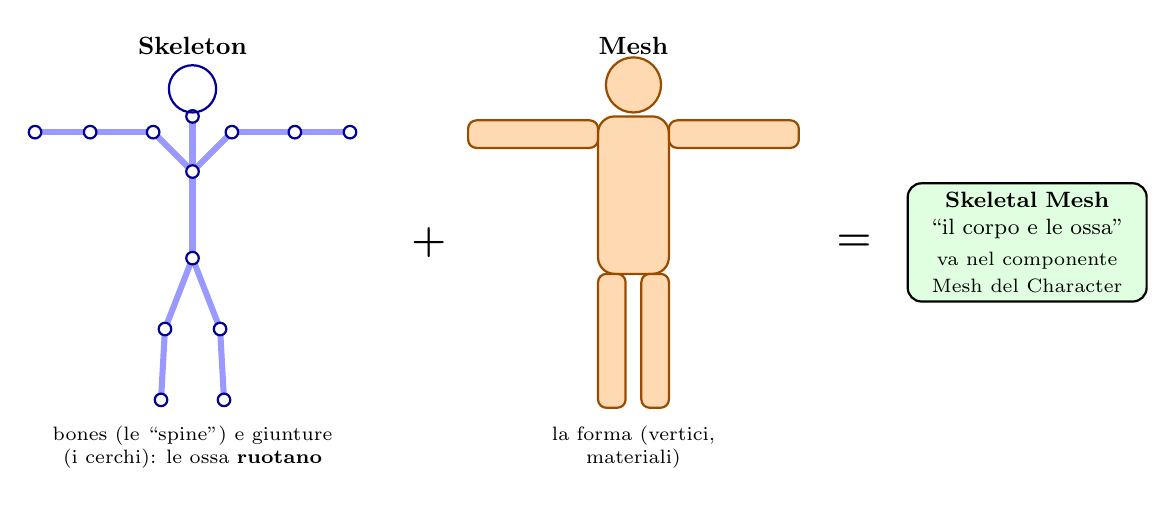
\begin{tikzpicture}[font=\footnotesize,
  ue8bone/.style={draw=blue!60!black, fill=blue!15, thick},
  ue8joint/.style={draw=blue!60!black, fill=white, thick, circle, inner sep=1.6pt}]
  % --- Skeleton (sinistra)
  \node[font=\small\bfseries] at (0,4.3) {Skeleton};
  \coordinate (pel) at (0,1.6); \coordinate (spi) at (0,2.7); \coordinate (nec) at (0,3.4);
  \coordinate (sl) at (-0.5,3.2); \coordinate (sr) at (0.5,3.2);
  \coordinate (el) at (-1.3,3.2); \coordinate (er) at (1.3,3.2);
  \coordinate (hl) at (-2.0,3.2); \coordinate (hr) at (2.0,3.2);
  \coordinate (kl) at (-0.35,0.7); \coordinate (kr) at (0.35,0.7);
  \coordinate (fl) at (-0.4,-0.2); \coordinate (fr) at (0.4,-0.2);
  \foreach \a/\b in {pel/spi, spi/nec, spi/sl, spi/sr, sl/el, sr/er, el/hl, er/hr,
                     pel/kl, pel/kr, kl/fl, kr/fr}
    \draw[ue8bone, line width=2.2pt, blue!40] (\a) -- (\b);
  \foreach \p in {pel, spi, nec, sl, sr, el, er, hl, hr, kl, kr, fl, fr}
    \node[ue8joint] at (\p) {};
  \draw[blue!60!black, thick] (0,3.75) circle (0.3);
  \node[font=\scriptsize, align=center] at (0,-0.8) {bones (le ``spine'') e
    giunture\\(i cerchi): le ossa \textbf{ruotano}};
  % --- piu'
  \node[font=\Large\bfseries] at (3.0,1.8) {+};
  % --- Mesh
  \begin{scope}[xshift=5.6cm]
    \node[font=\small\bfseries] at (0,4.3) {Mesh};
    \fill[orange!30, draw=orange!60!black, thick, rounded corners=6pt]
      (-0.45,1.4) rectangle (0.45,3.4);
    \fill[orange!30, draw=orange!60!black, thick] (0,3.8) circle (0.35);
    \fill[orange!30, draw=orange!60!black, thick, rounded corners=3pt]
      (-2.1,3.0) rectangle (-0.45,3.35);
    \fill[orange!30, draw=orange!60!black, thick, rounded corners=3pt]
      (0.45,3.0) rectangle (2.1,3.35);
    \fill[orange!30, draw=orange!60!black, thick, rounded corners=3pt]
      (-0.45,-0.3) rectangle (-0.1,1.4);
    \fill[orange!30, draw=orange!60!black, thick, rounded corners=3pt]
      (0.1,-0.3) rectangle (0.45,1.4);
    \node[font=\scriptsize, align=center] at (0,-0.8) {la forma (vertici,\\materiali)};
  \end{scope}
  % --- uguale
  \node[font=\Large\bfseries] at (8.4,1.8) {=};
  \node[draw, thick, rounded corners=5pt, fill=green!12, align=center, text width=2.8cm]
    at (10.6,1.8) {\textbf{Skeletal Mesh}\\``il corpo e le ossa''\\[2pt]
    \scriptsize va nel componente Mesh del Character};
\end{tikzpicture}
\caption{Skeletal Mesh e Skeleton secondo la lezione: due asset diversi. Lo Skeleton è
la gerarchia delle ossa, con le giunture; la Skeletal Mesh è la forma legata a quelle
ossa. Le animazioni sono rotazioni delle ossa, e sono legate allo Skeleton. Schema
ricostruito, non in scala.}
\label{ue8:fig:skeletal}
\end{figure}

\paragraph{Approfondimento: perché due asset.} Romero e Sewell (capitolo 17, ``Animation
Blueprints'') spiegano la separazione così: ``uno Skeleton è una gerarchia di ossa
interconnesse, usata per animare i vertici poligonali di una Skeletal Mesh''; e
``siccome l'animazione è fatta sullo Skeleton, può essere condivisa da molte Skeletal
Mesh che usano lo stesso Skeleton''. È il motivo per cui un gioco può avere decine di
personaggi diversi con un solo set di animazioni, e il motivo per cui, più avanti, le
animazioni del manichino di Unreal potranno essere \emph{ritargettate} sul cavaliere di
Mixamo, che ha uno scheletro simile ma non identico. Gli autori elencano anche i cinque
editor che si aprono dagli asset di animazione, con i bottoni in alto a destra già visti
dal docente: \emph{Skeleton Editor}, \emph{Skeletal Mesh Editor}, \emph{Animation
Editor}, \emph{Animation Blueprint Editor} e \emph{Physics Asset Editor}.

% ---------------------------------------------------------------------
\section{Le animazioni di Mixamo}
\label{ue8:sec:mixamoanim}

``Torniamo su Mixamo.'' L'importante è che nella viewport di Mixamo ci sia il proprio
personaggio, ``non un altro''; poi si passa alla categoria \textbf{Animations}. Servono
\textbf{tre animazioni} principali: \textbf{idle}, \textbf{walk} e \textbf{run}. ``La
idle, per chi non lo sapesse, sono le animazioni di stallo'': il personaggio ``sta fermo,
sta respirando'', il \emph{breathing}.

\paragraph{I controlli di Mixamo.} Sulla destra, per ogni animazione, ci sono alcuni
cursori; il docente li prova su animazioni diverse per farli vedere bene:
\begin{itemize}
  \item \textbf{Overdrive}: la velocità dell'animazione. ``Se aumento l'overdrive,
        questa animazione si velocizza sempre di più; se lo diminuisco, sarà
        lentissima'';
  \item \textbf{Character Arm-Space}: su alcuni modelli, la distanza delle braccia dal
        corpo, ``diventa sempre di più oppure diminuisce''. Attenzione al
        \emph{clipping}, le braccia che entrano nel corpo: ``infatti clippa
        malissimo''. Il docente suggerisce valori intorno a 50;
  \item \textbf{Trim}: ``tagliare l'animazione'', prenderne solo un pezzo. Ma ``viene
        fuori malissimo, perché non c'è il ritorno all'idle'': l'animazione tagliata non
        si chiude su sé stessa;
  \item \textbf{Mirror}: presente solo su alcune animazioni, ``semplicemente flippa
        l'animazione'', la \emph{specchia}. Il docente lo mostra con una Capoeira.
\end{itemize}

\paragraph{Root motion e in place.} Il punto più importante. Il docente apre un
\emph{Walking}: ``vedete che il character sta andando dritto, cioè sta percorrendo dello
spazio''. ``Questa tipologia di animazione viene chiamata \textbf{root motion}'': le
animazioni in root motion ``ereditano il movimento già nell'animazione''. L'esempio è
\emph{Dark Souls 3} (``qualcuno ha giocato Dark Souls 3? Perfetto''): alcune armi hanno
abilità speciali, le \emph{weapon art}, e in un video il docente cerca quella della
\emph{Holy Sword} (``questa non è in root motion, perché sta ferma''; ``eccola, questa
qua''): ``quando io la compio, mi sposto nello spazio già nell'animazione''. ``Non sono
io che gli do il movimento quando premo il tasto'': ``metto il piede in avanti, o faccio
l'affondo'', e il personaggio avanza perché lo fa l'animazione. Le animazioni in root
motion ``spesso sono usate per abilità'' di questo tipo.

``In questo caso, però, su Mixamo non dobbiamo avere un'animazione root motion'', perché
``erediteremmo un movimento che non ci interessa''. ``Noi, a livello del nostro gioco su
Unreal, vogliamo che l'animazione si compia, ma quella che si muove è la
\textbf{capsula}'': ``l'animazione segue la capsula''; ``c'è la mesh con l'animazione su
quella capsula, e di conseguenza si crea il movimento, o l'illusione del movimento''.
Quindi si spunta \textbf{In Place}: ``come potete vedere, adesso l'animazione è sul
posto''. ``Se non trovate una spunta In Place, consiglio di cambiare animazione: ce ne
sono tante'' (figura~\ref{ue8:fig:rootmotion}).

\begin{figure}[htbp]
\centering
\begin{tikzpicture}[font=\footnotesize,
  ue8cap/.style={draw=blue!60!black, thick, rounded corners=7pt, minimum width=0.7cm,
                 minimum height=1.6cm},
  ue8arr/.style={-{Stealth[length=2.4mm]}, very thick}]
  % root motion
  \node[font=\small\bfseries, anchor=west] at (-0.6,2.2) {Root motion};
  \node[ue8cap, fill=blue!8] at (0.3,0.9) {};
  \fill[orange!60] (0.3,1.5) circle (0.14);
  \draw[orange!60!black, very thick] (0.3,1.35) -- (0.3,0.75) -- (0.1,0.2);
  \draw[orange!60!black, very thick] (0.3,0.75) -- (0.5,0.2);
  \foreach \x/\o in {1.6/40, 2.9/60, 4.2/100} {
    \fill[orange!\o] (\x,1.5) circle (0.14);
    \draw[orange!\o!black, very thick] (\x,1.35) -- (\x,0.75) -- (\x-0.2,0.2);
    \draw[orange!\o!black, very thick] (\x,0.75) -- (\x+0.25,0.2);
  }
  \draw[ue8arr, orange!70!black] (0.6,-0.2) -- node[below, font=\scriptsize]
    {è l'animazione a spostare la mesh} (4.4,-0.2);
  \node[font=\scriptsize, align=left, text width=4.6cm, anchor=west] at (-0.6,-1.2)
    {la capsula resta indietro: mesh e collisione si separano. Utile per affondi e
    abilità (le weapon art di \emph{Dark Souls 3}), con Enable Root Motion};
  % in place
  \begin{scope}[xshift=7.4cm]
    \node[font=\small\bfseries, anchor=west] at (-0.6,2.2) {In place};
    \foreach \x/\o in {0.3/40, 1.6/60, 2.9/80, 4.2/100} {
      \node[ue8cap, fill=blue!8] at (\x,0.9) {};
      \fill[orange!\o] (\x,1.5) circle (0.14);
      \draw[orange!\o!black, very thick] (\x,1.35) -- (\x,0.75) -- (\x-0.2,0.2);
      \draw[orange!\o!black, very thick] (\x,0.75) -- (\x+0.25,0.2);
    }
    \draw[ue8arr, blue!60!black] (0.6,-0.2) -- node[below, font=\scriptsize]
      {è il Character Movement a spostare la capsula} (4.4,-0.2);
    \node[font=\scriptsize, align=left, text width=4.6cm, anchor=west] at (-0.6,-1.2)
      {l'animazione cammina sul posto, e la mesh segue la capsula: è quello che serve per
      idle, walk e run};
  \end{scope}
\end{tikzpicture}
\caption{Root motion e in place. In un'animazione root motion lo spostamento è dentro
l'animazione; in un'animazione in place il personaggio cammina sul posto, e a muoversi
nel mondo è la capsula del Character. Per la locomozione di base la lezione usa solo
animazioni in place. Schema ricostruito.}
\label{ue8:fig:rootmotion}
\end{figure}

\paragraph{Le impostazioni di download.} Al download Mixamo chiede alcune opzioni
(tabella~\ref{ue8:tab:mixamo}):
\begin{itemize}
  \item \textbf{Format}: \textbf{FBX Binary}, ``ci va bene così'';
  \item \textbf{Frames per Second}: \textbf{30}. ``Le animazioni devono essere allo
        stesso tipo di frame'': ``meglio sempre prenderle tutte quante allo stesso
        numero di frame'', ``perché se no avete dei problemi'', soprattutto ``nel
        \emph{blending}, cioè nel mixare'' due animazioni con frame rate diversi;
  \item \textbf{Skin}: \textbf{Without Skin}. ``La skin è se volete prendere
        l'animazione con il modello: non ci interessa, perché il modello ce l'abbiamo
        già'';
  \item \textbf{Keyframe Reduction}: \textbf{none}, ``non ci interessa'' ridurre i
        keyframe.
\end{itemize}
Il docente scrive in chat le tre animazioni da cercare, ``idle, walk e run/sprint'',
lasciando ``la libertà di scegliere quelle che volete'': ``importante che abbiate
un'animazione che respira, sta fermo, eccetera, una che cammina e una che fa lo
sprint''. Lui ha preso \emph{Idle}, \emph{Walking} e \emph{Slow Run}. ``Vi lascio 5, 10
minuti.''

\begin{table}[htbp]
\centering
\small
\begin{tabular}{@{}p{3.2cm}p{3.6cm}p{7.2cm}@{}}
\toprule
\textbf{Opzione} & \textbf{Valore} & \textbf{Perché} \\
\midrule
\multicolumn{3}{@{}l}{\emph{Personaggio}} \\
Format & FBX Binary & il formato che Unreal importa \\
Pose & T-Pose & la posa di riferimento del rig; togliere l'animazione applicata (la X) \\
\midrule
\multicolumn{3}{@{}l}{\emph{Animazioni (idle, walk, run)}} \\
Format & FBX Binary & come sopra \\
Skin & Without Skin & il modello c'è già: serve solo il movimento delle ossa \\
Frames per Second & 30 & tutte allo stesso frame rate, per non avere problemi nel
blending \\
Keyframe Reduction & none & nessuna riduzione dei keyframe \\
In Place & spuntato & niente root motion: a muoversi è la capsula \\
Overdrive, Arm-Space, Trim, Mirror & a piacere & velocità, distanza delle braccia
(attenzione al clipping), taglio, specchio \\
\bottomrule
\end{tabular}
\caption{Le impostazioni di download di Mixamo indicate a lezione.}
\label{ue8:tab:mixamo}
\end{table}

\paragraph{Approfondimento: Mixamo e Unreal.} Mixamo è un servizio gratuito di Adobe, a
cui si accede con un account Adobe; personaggi e animazioni si possono usare anche in
progetti commerciali. Il suo rig ha una gerarchia simile a quella del manichino di
Unreal (Manny e Quinn), ma i nomi delle ossa sono diversi (le ossa di Mixamo hanno il
prefisso \emph{mixamorig:}), e manca un osso \emph{root} alla base, sotto il bacino.
Per questo le animazioni di Mixamo in root motion non funzionano bene in Unreal senza
correzioni: lo spostamento è registrato sull'osso del bacino (\emph{Hips}) invece che su
un root. Con le animazioni \emph{In Place}, come quelle della lezione, il problema non si
pone. La mancanza dell'osso root e i nomi diversi sono anche il motivo per cui, per usare
sul cavaliere le animazioni del manichino (il salto, la caduta), servirà il
\textbf{retargeting} annunciato dal docente, con gli asset \emph{IK Rig} e \emph{IK
Retargeter} di Unreal Engine 5.

% ---------------------------------------------------------------------
\section{Importare le animazioni sullo scheletro}
\label{ue8:sec:importanim}

Dopo i minuti di scelta (``ci siete tutti, ragazzi? Sì, perfetto'') si importano le
animazioni. I file scaricati hanno il nome dell'animazione (``slow run, walking,
eccetera''); ``l'importante è che ci sia FBX sopra''. Al docente una delle due versioni
di Walking era rotta, e usa \emph{Walking 1}. ``Consiglio: fate meglio una cartella'':
\textbf{Animation}. ``Fatela una per una, vi consiglio.''

\paragraph{Lo scheletro obbligatorio.} La finestra di import è ``praticamente la stessa
schermata'', ``ma differenza sostanziale'': in basso, \textbf{Import} è grigio, non si
può premere. ``Per l'animazione in particolare gli serve uno scheletro a cui adattare
l'animazione.'' Nella sezione \textbf{Common} c'è il campo \textbf{Skeleton}: si apre la
tendina, in cui compaiono ``tutti gli scheletri'', compreso quello del manichino ``che
usiamo per Unreal'', e si sceglie \emph{il proprio}, quello creato dall'import del
personaggio. ``A questo punto, Import vi diventa blu.'' Nella stessa finestra il docente
indica anche la spunta sull'import della sola animazione (nella trascrizione: ``fate sì
che Import Only Animation sia ok''); la frase che segue è confusa.

\paragraph{Targettare.} ``Ecco a voi che si è creata un'animazione.'' ``Il file di per sé
è a parte, però lui ha \textbf{targettato}'' (``prendete questo termine'') ``la nostra
animazione su quello scheletro in particolare''. Un'animazione appartiene a uno
scheletro, e si può usare solo con le mesh di quello scheletro.

\paragraph{Approfondimento: le opzioni di import di un'animazione.} Nella finestra FBX
di Unreal Engine 5, quando il campo \emph{Skeleton} è impostato e la spunta
\emph{Import Mesh} è tolta, Unreal importa \emph{solo} le animazioni contenute nel file,
senza creare un'altra Skeletal Mesh e un altro scheletro; con \emph{Import Animations}
attivo, ogni animazione diventa un asset \textbf{Animation Sequence}. È il caso dei file
di Mixamo scaricati \emph{Without Skin}, che contengono solo le ossa animate. Se invece
si lascia vuoto il campo Skeleton su un file con la mesh, Unreal crea uno scheletro nuovo
a ogni import: è facile ritrovarsi con due scheletri quasi identici (``mi sa che ci sono
due ragazzi che hanno importato due'' scheletri, osserva il docente sulla sua tendina) e
con animazioni non compatibili fra loro.

% ---------------------------------------------------------------------
\section{L'editor dell'animazione}
\label{ue8:sec:animeditor}

Con un doppio clic sull'animazione si apre l'\textbf{Animation Editor}, ``che vi permette
di visualizzare tutte le particolarità della nostra animazione''.

\paragraph{I controlli.} In basso c'è il pannello di controllo: andare al primo o
all'ultimo frame (\emph{To Front}, \emph{To End}), al frame precedente o successivo
(``frame per frame per frame''). ``Le animazioni sono costituite da frame'': questa ne ha
\textbf{30}. Con \textbf{spazio}, o con il pulsante, \emph{Play} e \emph{Pause}.

\paragraph{Asset Details.} Sul lato dell'editor c'è il pannello \textbf{Asset Details}
(``se non vedete una finestra, la potete trovare su Window $\rightarrow$ Asset Details'',
``o Finestra $\rightarrow$ Dettagli dell'asset, suppongo, in italiano''). Ci sono molti
dati ``che nessuno andrebbe a vedere''; le cose principali:
\begin{itemize}
  \item \textbf{Loop}: ``se questa animazione la vogliamo che vada in loop'': ``quando
        finisce, ricomincia'';
  \item \textbf{Rate Scale}: a 1 è la velocità normale; ``se metto 1,5 l'animazione è
        più veloce''; a 2 ancora di più; ``40, diventa un casino''. ``È un po' come
        l'overdrive che abbiamo visto'' su Mixamo;
  \item \textbf{Root Motion}: la spunta \emph{Enable Root Motion} non è attiva, ``va
        bene così'', perché l'animazione è in place.
\end{itemize}
Lo stesso per le altre due animazioni: Idle, Slow Run (``vi chiederà sempre lo
scheletro''). ``Se aprite le vostre animazioni, sono giuste, sono davanti a voi?'' Alla
fine: ``dovreste avere tutte e tre le nostre belle animazioni''.

% ---------------------------------------------------------------------
\section{L'Animation Blueprint}
\label{ue8:sec:abp}

``La domanda sorge spontanea: come facciamo a metterle su un character?'' Con
l'\textbf{Animation Blueprint}.

\paragraph{La creazione.} Nella cartella del personaggio (il docente l'ha chiamata
\textbf{Characters}) si crea una cartella \textbf{Blueprint}. Poi tasto destro,
\textbf{Animation $\rightarrow$ Animation Blueprint}. La finestra chiede ``di quale
scheletro'': si sceglie il proprio (il docente, ``il mio paladino''), \textbf{Create}, e il
nome: \textbf{ABP\_Knight}, con il prefisso ABP per \emph{Animation Blueprint} (``io ho
chiamato Knight, però voi chiamatelo Ciccio Baciccio''). A uno studente che non ha
capito, il docente ripete: ``Animation, Animation Blueprint; vi chiederà lo scheletro;
selezionate lo scheletro vostro''. L'Animation Blueprint ``sarà la logica, quindi la
parte di programmazione'' delle animazioni ``del nostro bellissimo nuovo character''.

\paragraph{L'editor.} ``L'Animation Blueprint è abbastanza pieno di roba'', ``ci si può
confondere facilmente''. Le parti:
\begin{itemize}
  \item a sinistra, la \textbf{preview}, con il cavaliere in T-pose: ``e va benissimo,
        perché è la sua forma base'';
  \item l'\textbf{AnimGraph}, con il blocco \textbf{Output Pose}: ``tutti i calcoli che
        andremo a fare di animazioni'' si collegano a lui, ``e questo blocco ci dice:
        guarda, esce fuori questa roba'';
  \item l'\textbf{Event Graph}, ``come ce l'abbiamo in un classico Blueprint'', dove si
        possono ``creare e prendere variabili, modificare cose''.
\end{itemize}
``Esistono due ambienti particolari'': nel primo, l'AnimGraph, ``si ragiona per quanto
riguarda le animazioni''; nel secondo, l'Event Graph, ``a livello di programmazione''.

\paragraph{I due dati che servono.} Nell'Event Graph si devono ricavare due cose dal
personaggio:
\begin{enumerate}
  \item la \textbf{velocità}, ``perché vogliamo che la nostra animazione di camminata e
        di corsa, o di idle, sia relativa alla velocità che abbiamo al momento col
        character''. ``C'è una comunicazione tra i dati di gioco, quindi il movimento, e
        le animazioni'': ``dato un certo valore di velocità, cambia l'animazione'';
  \item se il personaggio \textbf{sta cadendo} o no, ``in modo da dire: guarda, sto
        saltando, sto iniziando a cadere; fammi un'animazione di salto, e fammi il loop
        del \emph{falling}''.
\end{enumerate}
Le animazioni di salto e caduta ``non le abbiamo importate'': ``le andremo a
ritargettare in seguito'', perché ``Unreal ci mette a disposizione la possibilità di
ritargettare delle animazioni'', ``ma non lo vedremo adesso''.

\paragraph{Event Blueprint Initialize Animation.} Il primo nodo è \textbf{Event Blueprint
Initialize Animation}: ``dice: quando l'animazione inizia''. ``Come abbiamo visto, gli
eventi come il Begin Play vengono fatti quando viene inizializzato tutto'': questo ``è il
Begin Play, ma per le animazioni''. (A questo punto Unreal si blocca di nuovo:
``è crashato Unreal; direi che oggi è proprio una gran roba''. ``Mi sa che mi tocca
svuotare un po' di memoria.'' Liberata la memoria, si riparte.)

\paragraph{Try Get Pawn Owner.} Dall'evento si chiama \textbf{Try Get Pawn Owner}.
``Questo blocco ci permette di comunicare con il nostro Pawn'', ``il nostro player''.
``Immaginatevi due ambienti separati'': nel Gameplay Framework ``il Pawn è quello che
controlla il character'', mentre l'animazione ``è subordinata al Pawn''. ``Quindi andiamo
a dire: ehi, provami a prendere l'owner, cioè il pawn owner.'' Poi ``andiamo a fare un
cast: abbiamo detto BP\_Knight\ldots{} Ah, giusto, ragazzi. Abbiamo scordato una cosa.
Dobbiamo creare effettivamente il nostro character.''

% ---------------------------------------------------------------------
\section{Il nuovo Character: BP\_Knight1}
\label{ue8:sec:character}

``Dobbiamo comunicare con il nostro character, per dire: guarda, mi servono questi dati
del movimento.'' Nella cartella Blueprint del personaggio: \textbf{Blueprint Class}, e
``attenzione'': come genitore si sceglie \textbf{Character}. Il nome:
\textbf{BP\_Knight1}.

\paragraph{I componenti del Character.} ``I character, a differenza degli actor, sono
costituiti di base da'':
\begin{itemize}
  \item un \textbf{Capsule Component}, la capsula;
  \item una \textbf{freccia} (\emph{Arrow}), ``per far capire qual è il forward vector
        della capsula'';
  \item la \textbf{Mesh}, una Skeletal Mesh;
  \item il \textbf{Character Movement}, ``il componente che definisce il movimento del
        character''. Nei suoi Details, in \emph{General Settings}, ci sono la
        \textbf{Gravity Scale}, la \textbf{Max Acceleration}, la \textbf{Braking
        Friction}. ``Come abbiamo detto, dobbiamo interfacciare le animazioni con i
        valori del movimento'', e quei valori stanno qui.
\end{itemize}

\paragraph{La Skeletal Mesh.} Nella Mesh si assegna la Skeletal Mesh del cavaliere (``devo
ricordarmi l'indirizzo''; ``no, non è questo, è questo qua''). Il personaggio ``è apparso
in modo abbastanza scorretto'', fuori posto rispetto alla capsula e girato male: ``basta
riposizionarlo''. ``Consiglio di fare lo \textbf{snapping}'': si abbassa la mesh in modo
che i piedi tocchino il fondo della capsula, e la si ruota ``in direzione della capsule'',
cioè con la faccia nella direzione della freccia (per i personaggi di Mixamo
serve di solito una rotazione di $-$90 gradi sulla Z; il valore esatto la trascrizione
non lo dice). ``Eccovi che abbiamo creato il nostro primo character.
Questa è la T-pose, meraviglioso.''

\paragraph{L'Anim Class.} ``Ma in questo caso non ha ancora animazioni.'' ``Come facciamo
a dire: guarda, devi usare proprio questa Animation Blueprint?'' Nella \textbf{Mesh}, alla
voce \textbf{Anim Class}, la tendina mostra tutti gli Animation Blueprint compatibili:
si sceglie \textbf{ABP\_Knight1} (il nome dell'asset del docente). ``Non è cambiato
niente, ma l'abbiamo messo in comunicazione'': quando l'Animation Blueprint avrà delle
animazioni, ``questo qua si aggiornerà''. La relazione è a due vie: il Character dice
quale Animation Blueprint usare (Anim Class), e l'Animation Blueprint chiede al suo
proprietario i dati (Try Get Pawn Owner).

% ---------------------------------------------------------------------
\section{Initialize: il cast e le referenze}
\label{ue8:sec:initialize}

Tornati nell'Animation Blueprint, il grafo dell'inizializzazione si completa
(figura~\ref{ue8:fig:abpgraph}, in alto):
\begin{enumerate}
  \item \textbf{Event Blueprint Initialize Animation};
  \item \textbf{Try Get Pawn Owner} $\rightarrow$ \textbf{Cast To BP\_Knight1}
        (``castate al vostro character, come l'avete chiamato'');
  \item dal pin As BP Knight1, \textbf{Promote to Variable}: una variabile referenza
        \textbf{BP\_Knight1}. ``Andiamo a creare una referenza del character, in modo
        tale che sia più semplice'': ``ogni volta che dovremmo prendere una cosa del
        character, dovremmo, se no, fare sempre Cast To BP\_Knight'', ed ``appesantisce
        castare sempre un qualcosa. Quindi lo facciamo all'inizio'';
  \item dalla referenza, \textbf{Get Character Movement}, ``per essere anche un po' più
        esaustivi'', e anche questo \textbf{Promote to Variable}: una variabile
        \textbf{MovementComponent}. ``Abbiamo creato già due variabili che ci faranno
        comodo in seguito.''
\end{enumerate}

\paragraph{Approfondimento: lo stesso grafo del modello Third Person.} Il grafo costruito
dal docente ricalca quasi nodo per nodo l'Animation Blueprint del manichino di Unreal
Engine 5 (\emph{ABP\_Manny}, nel modello Third Person): sull'Initialize, Try Get Pawn
Owner, Cast To Character, Set \emph{Character}, Get Character Movement, Set
\emph{MovementComponent}; sull'Update, controllo di validità, poi Set \emph{Velocity},
Set \emph{GroundSpeed} (Vector Length XY), Set \emph{ShouldMove} e Set \emph{IsFalling}.
La differenza è il cast: il modello fa Cast To \emph{Character}, la classe generica,
così che lo stesso Animation Blueprint funzioni con qualsiasi personaggio basato su
Character; la lezione fa Cast To BP\_Knight1, che dà accesso anche alle variabili
aggiunte nel cavaliere (utile, per esempio, per uno sprint), ma lega l'ABP a quella
classe.

% ---------------------------------------------------------------------
\section{Update: la velocità e la caduta}
\label{ue8:sec:update}

\paragraph{Event Blueprint Update Animation.} ``Questo evento avviene quasi come il Tick,
a ogni frame.'' ``Quando un'animazione si aggiorna, qualsiasi micro movimento è un
Update'': ``se abbiamo un idle, comunque è un'animazione; un walk, comunque è
un'animazione; e il run, comunque è un'animazione'', ``quindi sarà sempre attivo''. ``È
per questo che non facciamo il cast qui'': ``se no farebbe ogni volta, ogni frame,
sempre molto pesante''.

\paragraph{Il Validated Get.} ``Dobbiamo vedere se questo character è valido.'' ``Vi
ricordate gli Is Valid? Se in una variabile c'è qualcosa dentro o non c'è.'' C'è ``una
cosa molto interessante'': si trascina nel grafo un \textbf{Get} della variabile
BP\_Knight1, tasto destro, \textbf{Convert to Validated Get}. Il Get ``normale'' prende la
variabile e basta; il Validated Get ``prende la variabile, e mette anche la
particolarità: se lo prendo ed è valido faccio questo, se non è valido faccio
quest'altro''. Ha un ingresso di esecuzione e due uscite, \textbf{Is Valid} e \textbf{Is
Not Valid}: un Get e un Is Valid in un nodo solo. Sull'uscita Is Valid il docente mette
una \textbf{Sequence} (``un Is Valid, Sequence'') per eseguire in ordine le operazioni
che seguono.

\paragraph{GroundSpeed.} ``Fondamentalmente andiamo a prendere il Movement Component'',
la variabile creata nell'Initialize, e da lì \textbf{Get Velocity}: ``la velocità attuale,
a ogni frame, del character movement''. È un vettore; ``ci interessa solamente il
movimento'' sul piano, ``non ci interessa se salta o meno'', ``quello ci interesserà in
altro modo''. Quindi il nodo \textbf{Vector Length XY}: ``la lunghezza del vettore
solamente sugli assi X e Y'', ``se l'asse X è avanti e dietro e l'asse Y è destra e
sinistra''. Il risultato è un \textbf{float}, e diventa, con \textbf{Promote to
Variable}, \textbf{GroundSpeed}: ``una variabile che rappresenta la nostra velocità
attuale''.

\paragraph{IsFalling.} ``Molto importante per sapere quando saltiamo o quando stiamo
cadendo'': dal Movement Component, il nodo \textbf{Is Falling}. ``Ce ne sono due'': uno è
quello del \emph{Nav Movement}; quello giusto ``deve essere blu all'inizio e rosso alla
fine'', cioè con l'ingresso target blu (il Character Movement) e l'uscita rossa (una
booleana). Il valore va in una variabile, \textbf{IsFalling}, aggiornata a ogni frame,
``in modo tale da sapere che movimento fargli fare'' nel ``giro di animazioni''.

\paragraph{Velocity.} ``Per il futuro, per altre cose che ci serviranno'', anche il
vettore della velocità si promuove a variabile: \textbf{Velocity}, ``così almeno ci sono
delle cose che vogliamo interfacciare con la velocità''. ``Adesso abbiamo tirato fuori la
nostra velocità attuale e il fatto se sta cadendo o meno.'' A uno studente il Get
Velocity non compare: è quello che si ottiene dal Movement Component, con il target
giallo e l'uscita gialla (un vettore); cercandolo in fondo alla lista, ``trovato''.

\begin{figure}[htbp]
\centering
\begin{tikzpicture}[font=\footnotesize,
  ue8node/.style={draw, thick, rounded corners=4pt, align=center, fill=gray!8,
                  minimum height=0.8cm, text width=2.0cm},
  ue8ev/.style={ue8node, fill=red!12},
  ue8pure/.style={ue8node, fill=green!10, rounded corners=8pt},
  ue8var/.style={ue8node, fill=blue!10, rounded corners=8pt},
  ue8exec/.style={-{Stealth[length=2.5mm]}, very thick, black!80},
  ue8data/.style={-{Stealth[length=2mm]}, thick, blue!60!black}]
  % Initialize
  \node[font=\small\bfseries, anchor=west] at (-1.2,1.3) {Inizializzazione (una volta)};
  \node[ue8ev, text width=2.3cm] (ini) at (0,0) {\textbf{Event Blueprint Initialize
    Animation}};
  \node[ue8node, fill=blue!10, text width=1.9cm] (cst) at (3.2,0) {\textbf{Cast To}\\
    BP\_Knight1};
  \node[ue8pure] (tgp) at (3.2,-1.6) {\textbf{Try Get}\\\textbf{Pawn Owner}};
  \node[ue8node, text width=2.0cm] (s1) at (6.2,0) {\textbf{Set}\\BP\_Knight1};
  \node[ue8node, text width=2.8cm] (s2) at (9.6,0) {\textbf{Set}\\Movement\-Component};
  \node[ue8pure, text width=2.6cm] (gcm) at (9.6,-1.6) {BP\_Knight1 $\rightarrow$\\
    \textbf{Get Character Movement}};
  \draw[ue8exec] (ini) -- (cst);
  \draw[ue8data] (tgp) -- node[right, font=\scriptsize]{Object} (cst);
  \draw[ue8exec] (cst) -- (s1);
  \draw[ue8exec] (s1) -- (s2);
  \draw[ue8data] (gcm) -- (s2);
  % Update
  \node[font=\small\bfseries, anchor=west] at (-1.2,-3.1) {Aggiornamento (ogni frame)};
  \node[ue8ev, text width=2.3cm] (upd) at (0,-4.6) {\textbf{Event Blueprint Update
    Animation}};
  \node[ue8var, text width=2.0cm] (vg) at (3.3,-4.6) {\textbf{Validated Get}\\
    BP\_Knight1};
  \node[ue8node, text width=1.6cm] (seq) at (6.5,-4.6) {\textbf{Sequence}};
  \node[ue8node, text width=3.6cm, align=left] (sv) at (10.6,-3.4) {\textbf{Set
    Velocity} $\leftarrow$\\MovementComponent $\rightarrow$ Get Velocity};
  \node[ue8node, text width=3.6cm, align=left] (sg) at (10.6,-4.7) {\textbf{Set
    GroundSpeed} $\leftarrow$\\Vector Length XY (Velocity)};
  \node[ue8node, text width=3.6cm, align=left] (sf) at (10.6,-6.0) {\textbf{Set
    IsFalling} $\leftarrow$\\MovementComponent $\rightarrow$ Is Falling};
  \draw[ue8exec] (upd) -- (vg);
  \draw[ue8exec] (vg) -- node[above, font=\scriptsize]{Is Valid} (seq);
  \draw[ue8exec] (seq.east) -- ++(0.4,0) |- node[pos=0.75, above, font=\scriptsize]
    {Then 0} (sv.west);
  \draw[ue8exec] (seq.east) -- ++(0.4,0) |- node[pos=0.75, above, font=\scriptsize]
    {Then 1} (sg.west);
  \draw[ue8exec] (seq.east) -- ++(0.4,0) |- node[pos=0.75, above, font=\scriptsize]
    {Then 2} (sf.west);
\end{tikzpicture}
\caption{I due grafi dell'Event Graph di ABP\_Knight. In alto, una sola volta: si prende
il proprietario, lo si converte nel cavaliere e si salvano due referenze. In basso, a
ogni frame: se la referenza è valida, si aggiornano Velocity (vettore), GroundSpeed (la
sua lunghezza sul piano XY) e IsFalling (booleana). Accanto a ogni Set, il valore che riceve.
Schema ricostruito.}
\label{ue8:fig:abpgraph}
\end{figure}

\paragraph{Un registro di dati.} ``Questo graph funziona letteralmente come'' un
registro (la trascrizione dice ``registri di credito''): serve ``principalmente per
interfacciarsi con il nostro bellissimo character'', e ``ci serve per capire valori,
vedere cose'', ``parliamo di numeri per lo più''. Le animazioni vere si decidono altrove.

\paragraph{Approfondimento: perché l'AnimGraph non legge da solo.} Romero e Sewell
(capitolo 17) descrivono la stessa divisione dei compiti: ``usiamo l'EventGraph di un
Animation Blueprint per prendere i dati dal Pawn o dal Character che sta usando l'istanza
dell'Animation Blueprint, e per aggiornare le variabili dell'Animation Blueprint''; e
``l'AnimGraph può accedere solo alle variabili dell'Animation Blueprint''. Il loro esempio
è più semplice di quello della lezione: sull'Update un Is Valid sul Try Get Pawn Owner,
Get Velocity dal Pawn, \emph{VectorLength} (la lunghezza su tutti e tre gli assi) e Set
di una variabile \emph{Speed}. La scelta del docente, \textbf{Vector Length XY}, è più
precisa per la locomozione: con la lunghezza completa, un personaggio che cade dritto
verso il basso avrebbe una velocità alta e farebbe la corsa a mezz'aria. Gli autori
notano anche che \emph{Event Blueprint Update Animation} ha un parametro \emph{Delta Time
X}, il tempo trascorso dall'ultimo frame, utile per interpolare i valori.

% ---------------------------------------------------------------------
\section{L'AnimGraph, un'anteprima del Blend Space e il personaggio finito}
\label{ue8:sec:animgraph}

``Adesso, ragazzi, vi faccio una spiegazione teorica molto corta, perché capisco che siamo
agli ultimi dieci minuti, anzi sette.'' L'AnimGraph, ``differentemente, lavora per
esempio per \emph{state machine}''.

\paragraph{Un'animazione sull'Output Pose.} Il caso più semplice: nell'\textbf{Asset
Browser} dell'editor (``qua trovate tutte le animazioni che sono compatibili con questo
scheletro'') si prende un'animazione, per esempio \emph{Walking 1}, la si trascina
nell'AnimGraph e si collega ``l'omino'' del nodo all'omino dell'\textbf{Output Pose}. Non
è in loop, ma basta spuntare \textbf{Loop Animation} nei Details del nodo. Compile: nella
preview il cavaliere cammina. ``E possiamo vederlo anche nel nostro character'', perché
l'Anim Class ``ci ha permesso di dirgli: guarda, ehi, hai questo in eredità, hai questo
sotto di te, l'Animation Blueprint''. ``Ma, come potete capire, a noi serve molto di più
rispetto a mettere queste animazioni'' una alla volta.

\paragraph{Il Blend Space 1D.} ``Sicuramente la prossima volta andremo a vedere quelli
che sono chiamati \textbf{Blend Space}. Ve lo faccio vedere velocissimamente.'' Il
docente apre un \textbf{Blend Space 1D} (``una dimensione''), creato sullo scheletro del
cavaliere: un grafico con il personaggio che ``ci permette di mettere insieme varie
animazioni che \emph{blendano} tra di loro'', cioè ``che interpolano tra di loro''.
Nella preview, spostandosi sull'asse: idle, poi walking, poi sprint. ``In questo caso ci
sarà solamente un asse, che noi diremo che sarà la nostra \textbf{GroundSpeed}'', la
velocità ``che definisce il movimento'' (figura~\ref{ue8:fig:blendspace}). ``La prossima
volta vedremo di costruire questa tipologia di asset e collegare tutto quanto.''

\begin{figure}[htbp]
\centering
\begin{tikzpicture}[font=\footnotesize,
  ue8pt/.style={draw=black, fill=white, thick, diamond, inner sep=2.2pt}]
  \draw[-{Stealth[length=2.5mm]}, thick] (0,0) -- (11.2,0) node[right]{GroundSpeed};
  \foreach \x/\v in {0/0, 2.5/150, 5/300, 7.5/450, 10/600}
    \draw (\x,0.1) -- (\x,-0.1) node[below, font=\scriptsize]{\v};
  \node[ue8pt] (i) at (0,0) {}; \node[ue8pt] (w) at (2.5,0) {}; \node[ue8pt] (r) at
    (10,0) {};
  \node[above=6pt of i, font=\scriptsize\bfseries] {Idle};
  \node[above=6pt of w, font=\scriptsize\bfseries] {Walking};
  \node[above=6pt of r, font=\scriptsize\bfseries] {Run / Sprint};
  \fill[green!50!black] (6.25,0) circle (0.12);
  \draw[green!50!black, thick, ->] (6.25,0.9) -- (6.25,0.2);
  \node[green!40!black, font=\scriptsize, align=center] at (6.25,1.3) {valore attuale:
    50\% Walking + 50\% Run};
  \node[font=\scriptsize, align=center, text width=11cm] at (5.5,-1.0) {le animazioni
    sono campioni posti sull'asse; fra due campioni Unreal le mescola in proporzione
    alla distanza};
\end{tikzpicture}
\caption{Un Blend Space 1D come quello mostrato in anteprima: un solo asse, la
GroundSpeed calcolata nell'Event Graph, e tre animazioni poste su di esso. I valori
sull'asse sono un esempio, non quelli del docente. Schema ricostruito.}
\label{ue8:fig:blendspace}
\end{figure}

\paragraph{Il personaggio finito.} Per chiudere, il docente mostra dove arriveranno.
``Io posso cambiare il nostro character da qui'': nei \textbf{World Settings} del livello,
nella Game Mode, alla voce \textbf{Default Pawn Class}, sceglie BP\_Knight. In Play, il
cavaliere si muove con idle, camminata e corsa, e ``gli ho messo addirittura pure lo
sprint''. ``Il salto, questo è ritargettato'': è l'animazione classica di Unreal, portata
sullo scheletro di Mixamo. E la vecchia logica funziona con il nuovo personaggio:
``possiamo fare tutte le interazioni, e addirittura la nostra torretta ci segue''.
``Questo lo faremo la prossima volta'', ``perché ci vuole un pochino di continuità''.

\paragraph{Approfondimento: dalle animazioni singole alla State Machine.} Il capitolo 17
di Romero e Sewell mostra i passi successivi, quelli annunciati per la prossima lezione.
Un \textbf{Blend Space} è ``un tipo di asset che permette di mescolare animazioni in base
ai valori di uno o due parametri'': nel loro esempio del modello Third Person (UE4), il
Blend Space di locomozione pone \emph{Idle} a 0, \emph{Walk} a 93,75 e \emph{Run} a 375,
e con una velocità di circa 234 l'animazione risultante è metà camminata e metà corsa.
Trascinato nell'AnimGraph, il Blend Space diventa un nodo \emph{Blendspace Player} con un
ingresso per il parametro, a cui si collega la variabile della velocità; nell'\emph{Anim
Preview Editor} si può cambiare il valore e vedere il risultato senza andare in Play.
Poi la \textbf{State Machine}: un nodo dell'AnimGraph che organizza le animazioni in
\emph{stati} (per esempio \emph{Idle} e \emph{Moving}, e più avanti \emph{Jump} e
\emph{Fall}), collegati da \emph{transizioni} con regole booleane (per esempio
``GroundSpeed $>$ 3'' per passare da fermo a in movimento, o ``IsFalling'' per passare
al salto). È lì che la variabile IsFalling di oggi troverà il suo uso.

% ---------------------------------------------------------------------
\section{I materiali mancanti e la chiusura}
\label{ue8:sec:chiusura}

``Ci sono domande, ragazzi?'' Una studentessa: ``il mio personaggio non c'ha un
materiale, ha solo le texture''. ``Anche il mio non è importato'', aggiunge un altro.

\paragraph{Creare il materiale a mano.} La studentessa condivide lo schermo: il suo
personaggio di Mixamo è un'arciera (\emph{Erika Archer}, a giudicare dalla trascrizione).
``Se non hai un materiale, dovresti crearlo da zero'':
\begin{enumerate}
  \item tasto destro $\rightarrow$ \textbf{Material}, chiamato \textbf{M\_Archer};
  \item aperto il materiale in una finestra piccola, si trascinano dentro tutte le
        \textbf{texture} (``quelle con il label rosso''), che diventano nodi
        \textbf{Texture Sample};
  \item si legge bene il nome di ognuna: la \textbf{Diffuse} va nel \textbf{Base Color}
        (``acciaccala in Base Color''); la \textbf{Normal} va nel \textbf{Normal}.
\end{enumerate}
Leggendo i nomi, però, si scopre che le texture sono di due gruppi: una Diffuse dei
\emph{vestiti} e una della \emph{pelle} (e una delle ciglia, l'\emph{eyelash}). ``Ha due
materiali diversi, forse.'' ``Quindi mi sa che devi fare due materiali: uno per i
vestiti, e l'altro per la pelle'', per esempio \emph{M\_ArcherClothing}.

\paragraph{Gli slot dei materiali.} Per sapere dove va cosa, si apre la Skeletal Mesh:
nei Details, la sezione dei materiali mostra gli slot, con il \textbf{WorldGridMaterial}
(la griglia grigia di default) dove manca un materiale. Gli slot sono \emph{quattro}, non
due. Si mette il nuovo materiale nell'\textbf{Element 0} e si guarda ``dove te lo mette sul
corpo'': passando sopra uno slot, la parte corrispondente si illumina
(\emph{highlight}). Element 0 è il \emph{clothing}; il 2 e il 3 saranno la pelle, con un
altro materiale. ``Tanto, se non avete i materiali ma avete le texture, ragazzi, potete
farlo direttamente a mano.''

\paragraph{Le texture che non ci sono.} A un altro studente non sono state importate
nemmeno le texture. Il docente prova a riprodurre il problema: torna su Mixamo (``Mixamo
non mi risponde più, ottimo''), scarica lo stesso personaggio, \emph{The Boss}
(``use this character''; ``madonna mia''), in T-pose, e lo importa. Nella finestra di
import, nella sezione dei materiali, \textbf{Import Materials} e \textbf{Import
Textures} devono essere attivi (``fai sì che i materiali siano importati''); \emph{Import
Morph Targets} e simili ``non ci interessano''. ``A me importa tutto.'' ``Se c'hai
difficoltà, magari puoi semplicemente riprovare a fare l'import.'' Intanto Federico ha
risolto da solo, assegnando i materiali agli slot con l'highlight: ``allora vuol dire che
ti sei risolto la vita da solo. Perfetto.''

\paragraph{Approfondimento: Diffuse, Normal e gli altri canali.} Una \textbf{Diffuse} (o
\emph{Albedo}, o \emph{Base Color}) è il colore della superficie senza luci né ombre, e
va nel pin Base Color; una \textbf{Normal map}, riconoscibile dal colore azzurro-violetto,
simula i rilievi e va nel pin Normal (Unreal la riconosce all'import e imposta la
compressione \emph{Normalmap}). Se ci sono texture di \emph{Specular}, \emph{Roughness} o
\emph{Gloss}, vanno nei pin corrispondenti, ricordando che una Gloss è l'inverso di una
Roughness (serve un nodo \emph{1-x}, \emph{OneMinus}). Per le ciglia e i capelli, fatti
di piani con trasparenze, il materiale va impostato con \emph{Blend Mode} \emph{Masked}
e l'alfa della texture collegata all'\emph{Opacity Mask}: altrimenti le ciglia appaiono
come rettangoli pieni. Sono gli stessi nodi visti nella terza lezione, dedicata a
texture e materiali.

\paragraph{La chiusura.} ``Altri problemi? Se no, ci sentiamo la prossima volta.''
``Se dovete dichiarare qualcosa, non alla dogana, spero, ci sentiamo su Discord'':
``mandatemi quello che volete, se provate cose''. A Filippo: ``poi magari ti guardo un po'
quelle cosette che abbiamo visto prima''. ``Allora, ragazzi, buona cena, buona serata.
Ci vediamo giovedì. Ciao, ciao.''

\begin{table}[htbp]
\centering
\small
\begin{tabular}{@{}p{5.4cm}p{8.6cm}@{}}
\toprule
\textbf{Sintomo} & \textbf{Causa e rimedio} \\
\midrule
Una variabile ``non si muove'' & creata di nuovo e rimasta al default (0): controllare i
valori; variabili con nomi chiari \\
Errore sull'Audio Component ``non valido'' (Set Pitch Multiplier), solo arrivando in
fondo & caso rimasto aperto; ipotesi: lo Stop distrugge il suono (Auto Destroy) e la
variabile resta a puntare al vuoto. Is Valid, o Auto Destroy disattivato, o reset del Do
Once \\
L'ascensore va sempre più giù e non risale & attivazioni ripetute: booleana Activated
(Branch sul False all'inizio di Activation, false sul Begin Overlap) \\
Il progetto non si apre (si apre solo Unreal) & probabile chiavetta USB staccata male:
rimuoverla in sicurezza; usare un sistema di versione (Git) \\
Il personaggio si ferma un istante sul collezionabile & doppia collisione: mesh in
NoCollision, resta la Sphere Collision \\
On Component Begin Overlap non compare & è selezionata la mesh e non la Collision \\
Get Collectables non compare da Get Game Instance & manca il Cast To GI\_Platform: la
referenza è generica \\
Il cast non funziona & Get Game Instance non collegato all'Object del cast \\
``Non eredita da istanza di gioco''; la classe non compare nei Project Settings & la
Game Instance è stata creata con un altro genitore: ricrearla da GameInstance, sceglierla
in Game Instance Class, rifare variabile e cast \\
Il collezionabile conta ma l'esecuzione si ferma & il filo di esecuzione non passa per
il cast \\
Open Level non carica il livello & nome scritto male: è case sensitive. Copiarlo con F2,
Ctrl+C, Ctrl+V \\
Le palline raccolte riappaiono & normale: il livello viene ricaricato. Salvare lo stato
nella Game Instance (esercizio futuro) \\
Mettere a terra un componente nel Blueprint & nessuna scorciatoia (End vale solo nel
livello): regolare la Z a mano \\
Errore su Set Play Rate all'uscita dal Play & una vecchia referenza alla timeline con lo
stesso nome: eliminarla e usare quella giusta \\
Unreal si chiude durante l'import & memoria video esaurita: liberare memoria e spazio su
disco, reimportare \\
Il personaggio importato è ruotato & Offset Rotation non a zero: controllare Offset
Translation e Rotation all'import \\
Import grigio per un'animazione & manca lo Skeleton: sceglierlo in Common
$\rightarrow$ Skeleton \\
L'animazione sposta il personaggio da sola & è in root motion: riscaricarla da Mixamo
con In Place \\
Get Velocity non compare & cercarlo dal Movement Component (target e uscita gialli) \\
Il personaggio di Mixamo è grigio, senza materiale & creare i materiali a mano (Diffuse
in Base Color, Normal in Normal) e assegnarli agli slot; o reimportare con Import
Materials e Import Textures \\
\bottomrule
\end{tabular}
\caption{I problemi incontrati durante la lezione, con la causa e il rimedio.}
\label{ue8:tab:errori}
\end{table}

\begin{table}[htbp]
\centering
\small
\begin{tabular}{@{}p{4.6cm}p{9.4cm}@{}}
\toprule
\textbf{Nodo, asset o impostazione} & \textbf{Che cosa fa} \\
\midrule
Game Instance (Blueprint Class) & l'oggetto che vive per tutto il gioco; contiene dati
globali \\
Project Settings $\rightarrow$ Maps \& Modes $\rightarrow$ Game Instance Class & sceglie
la Game Instance del progetto \\
Get Game Instance & restituisce la Game Instance, come referenza generica \\
Cast To (classe) & converte una referenza nel tipo specifico; Cast Failed se non lo è \\
Increment Int (++) / Decrement Int ($--$) & aggiunge o toglie 1 a una variabile intera \\
Collision Presets: NoCollision & toglie ogni collisione a un componente \\
Sphere Collision, Sphere Radius & volume sferico e il suo raggio \\
Destroy Actor & distrugge l'actor \\
Evento Key (E) & scatta alla pressione di un tasto (Pressed, Released) \\
Text Render & un testo nel mondo 3D \\
Hidden in Game & nasconde un componente in gioco; tolto, la box si vede \\
Open Level (by Name) & carica un livello dal nome (case sensitive) \\
File $\rightarrow$ New Level (Basic) & un livello con cielo, luce e pavimento \\
Skeletal Mesh / Skeleton / Physics Asset & la mesh con le ossa; la gerarchia delle ossa;
i corpi fisici \\
Offset Translation / Rotation (import) & posizione e rotazione dell'asset rispetto al
pivot \\
Animation Sequence: Loop, Rate Scale, Enable Root Motion & ripetizione, velocità,
movimento dentro l'animazione \\
Animation Blueprint (ABP) & la logica delle animazioni di uno scheletro: Event Graph e
AnimGraph \\
Anim Class (Mesh del Character) & l'Animation Blueprint usato dalla mesh \\
Character (Capsule, Arrow, Mesh, Character Movement) & il Pawn che cammina, salta,
nuota, vola \\
Event Blueprint Initialize Animation & il ``Begin Play'' dell'Animation Blueprint \\
Try Get Pawn Owner & il Pawn che usa l'Animation Blueprint \\
Event Blueprint Update Animation & scatta a ogni aggiornamento dell'animazione, come il
Tick \\
Convert to Validated Get & un Get con le uscite Is Valid e Is Not Valid \\
Sequence & esegue più uscite in ordine \\
Get Velocity / Vector Length XY & la velocità; la sua lunghezza sul piano \\
Is Falling (Character Movement) & vero se il personaggio è in aria \\
Output Pose (AnimGraph) & la posa finale applicata alla mesh \\
Blend Space 1D & mescola animazioni lungo un asse (GroundSpeed) \\
World Settings $\rightarrow$ Default Pawn Class & il personaggio del giocatore in quel
livello \\
\bottomrule
\end{tabular}
\caption{I nodi, gli asset e le impostazioni dell'ottava lezione.}
\label{ue8:tab:nodi}
\end{table}

% ---------------------------------------------------------------------
\section*{Punti chiave del capitolo}
\addcontentsline{toc}{section}{Punti chiave del capitolo}

\begin{itemize}
  \item Il \textbf{Gameplay Framework} è la gerarchia delle entità che Unreal crea mentre
        il gioco gira: \textbf{Game Instance} (per tutta la durata del gioco), livello,
        \textbf{Game Mode} (le regole), \textbf{Game State} e \textbf{Player State} (lo
        stato, condiviso in rete), \textbf{Player Controller} (il ``cervello'' non
        fisico), \textbf{Pawn} e \textbf{Character} (il ``corpo''), e infine l'input.
  \item \textbf{Pubblica non vuol dire globale}: le variabili degli actor muoiono con il
        livello. Per conservare dati fra i livelli si usa la \textbf{Game Instance},
        creata come Blueprint Class da GameInstance e scelta in \textbf{Project Settings
        $\rightarrow$ Maps \& Modes $\rightarrow$ Game Instance Class}. Non va
        appesantita, perché resta in memoria per tutta la partita.
  \item \textbf{Get Game Instance} restituisce una referenza generica, ``la scocca'':
        per leggere le nostre variabili serve il \textbf{Cast To} della nostra classe,
        ``l'abito giusto'' per entrare alla festa. Cast Failed non è un errore, è una
        risposta.
  \item Un \textbf{collezionabile}: Sphere Collision, mesh in \textbf{NoCollision} (niente
        doppia collisione), controllo sul player, \textbf{Increment Int} sulla variabile
        della Game Instance, \textbf{Destroy Actor}.
  \item Un volume che cambia livello: \textbf{Open Level (by Name)} con il nome promosso
        a variabile pubblica. I nomi sono \textbf{case sensitive}: copiarli con F2 e
        Ctrl+C. I livelli nuovi da \textbf{File $\rightarrow$ New Level $\rightarrow$
        Basic}, salvati subito con Ctrl+S.
  \item Una booleana \textbf{Activated} con un Branch fa da cancello: l'ascensore
        ignora le attivazioni ripetute finché il player non lo fa risalire.
  \item Una \textbf{Skeletal Mesh} è ``il corpo e le ossa''; lo \textbf{Skeleton} è un
        asset separato, a cui sono legate le animazioni. Le ossa si \textbf{ruotano},
        non si spostano.
  \item Da \textbf{Mixamo}: personaggio in \textbf{T-pose}, \textbf{FBX Binary};
        animazioni idle, walk e run \textbf{In Place} (non root motion: a muoversi è la
        capsula), \textbf{Without Skin}, \textbf{30 fps} per tutte, nessuna riduzione dei
        keyframe. All'import si controllano gli \textbf{Offset}; le animazioni si
        importano scegliendo lo \textbf{Skeleton}.
  \item L'\textbf{Animation Blueprint} ha due grafi: l'\textbf{Event Graph} raccoglie i
        dati dal personaggio, l'\textbf{Anim\-Graph} decide la posa (\textbf{Output
        Pose}). Il Character lo usa tramite l'\textbf{Anim Class} della Mesh.
  \item Nell'\textbf{Initialize}: Try Get Pawn Owner, Cast To del personaggio, e le
        referenze salvate in variabili (il cast una volta sola). Nell'\textbf{Update},
        che gira a ogni frame: \textbf{Validated Get}, poi \textbf{GroundSpeed} (Vector
        Length XY della Get Velocity), \textbf{IsFalling} e \textbf{Velocity}.
  \item Prossimi passi: il \textbf{Blend Space 1D} sulla GroundSpeed, la State Machine,
        il \textbf{retargeting} del salto, e il personaggio impostato come
        \textbf{Default Pawn Class}.
\end{itemize}

%
%  Tutte le etichette di questo capitolo hanno il prefisso "ue8:"
%  (ue8:cap:..., ue8:sec:..., ue8:fig:..., ue8:tab:...), e tutti gli
%  stili TikZ hanno il prefisso "ue8" (ue8node, ue8exec, ue8data, ...)
%  per non collidere con chiavi native di TikZ né con quelli delle
%  lezioni precedenti. Il capitolo è autonomo: non contiene \ref verso
%  altri capitoli (i rimandi alle lezioni precedenti sono a parole).
%  Le figure sono ricostruzioni schematiche di quanto mostrato e detto a
%  lezione, non copie delle slide o delle schermate del docente. Dove la
%  trascrizione è troppo rovinata per ricostruire un dettaglio, il
%  capitolo lo dice invece di inventarlo.
% =====================================================================

\chapter[Game Instance, livelli e animazioni]{Game Instance, livelli e animazioni: il
Gameplay Framework e un nuovo personaggio}
\label{ue8:cap:gameinstance}

Questa è l'\textbf{ottava lezione} del corso breve di \textbf{introduzione a Unreal
Engine}. Nelle sette lezioni precedenti tutto è avvenuto dentro un solo livello e con un
solo personaggio, il manichino del modello Third Person: la torretta, i proiettili, la
piattaforma che sale, il pulsante che attiva le luci. Oggi la lezione allarga lo sguardo
in due direzioni. La prima è \textbf{uscire dal livello}: cambiare mappa senza perdere
quello che il giocatore ha fatto, cioè \textbf{salvare dei valori in modo globale}. La
seconda è \textbf{cambiare personaggio}: prendere un modello nuovo da \textbf{Mixamo},
importarlo con il suo scheletro e le sue animazioni, e cominciare a costruire la logica
che decide quale animazione mostrare, l'\textbf{Animation Blueprint}.

Il filo che tiene insieme le due parti è il \textbf{Gameplay Framework} di Unreal: la
``gerarchia'' delle entità che l'engine crea e tiene in vita mentre il gioco gira. La
\textbf{Game Instance}, la prima a nascere e l'ultima a morire, è il posto giusto per i
dati che devono sopravvivere al cambio di livello; il \textbf{Pawn} e il
\textbf{Character}, con il loro \textbf{Character Movement}, sono la fonte dei dati
(velocità, caduta) che l'Animation Blueprint legge per animare lo scheletro. ``Andremo
sia a vedere quelle che sono le animazioni e come si gestiscono, ma sia a vedere un po'
quello che è chiamato il \emph{gameplay framework} di Unreal.''

La lezione è \textbf{online}, su Zoom, come le precedenti, ma con una particolarità: la
webcam del docente si rifiuta di funzionare per tutta la serata (``oggi mi vedrete con
uno schermo nero, o almeno il mio schermo è più importante della mia faccia''), e in
due occasioni l'editor si chiude da solo per mancanza di memoria video. Si apre con un
problema di uno studente rimandato alla pausa, prosegue con una parte teorica in slide
sul Gameplay Framework e con la costruzione dei collezionabili, della Game Instance e
dei volumi che cambiano livello; la pausa arriva verso le 17:26, con ripresa alle ``55,
18, solito orario''; la seconda parte è dedicata all'import del personaggio e delle
animazioni e all'Animation Blueprint. Il docente stesso avverte che non si arriverà in
fondo: ``probabilmente questa lezione la riporteremo nella prossima'', in cui si vedranno
i Blend Space e il resto delle animazioni. Si chiude con un ``ci vediamo giovedì''.

Tre avvertenze di lettura, le stesse delle lezioni precedenti. La prima: la
trascrizione è automatica e storpia moltissimi nomi. Unreal è ``Arena Engine'',
``Arreal'', ``a Real'', ``a RIAL'', ``Arial'' e ``Irium'' (quest'ultimo, forse, è il
programma della webcam); la \textbf{Game Instance} è ``View Instance'', ``getViewInstance''
e ``key instance''; \textbf{GI\_Platform} è ``GI Gaming Instance'', ``gi i platform'',
``asg.platform'', ``giiPatform'' e ``Di Alto''; il \textbf{Pawn} è ``Pwn'', ``la Bone'' e
``player born''; \textbf{Get Player Pawn} è ``getLayerOne'' e ``PlayerOh''; il
\textbf{Cast To} è ``castagna''; l'\textbf{On Component Begin Overlap} è ``component
baking per l'acqua'', ``onBegin onComponent onBegin overlap'' e ``On Collision Beginner
per l'app''; il \textbf{Destroy Actor} è ``destroy hardware''; il \textbf{Text Render} è
``text rendere''; la \textbf{Skeletal Mesh} è ``scheletal mesh'' e ``scheda del Mesh''; il
\textbf{Control Rig} è ``control righe''; l'\textbf{Idle} è ``Idol''; il \textbf{root
motion} è ``root in''; la \textbf{T-pose} è ``Tico'', ``tifoso'' e ``Bix ti pose'';
\textbf{FBX Binary} è ``Fibix binary''; il \textbf{Knight} è ``Night''; il \textbf{Try Get
Pawn Owner} è ``try get one''; l'\textbf{Event Blueprint Update Animation} è ``event
blueprint a data animation''; \textbf{IsFalling} è ``isPalling''; il \textbf{Diffuse} è
``Diffuse'', ma l'\textbf{eyelash} è ``ailash''; \textbf{Mixamo} è a volte
``Mixamon''. Dove la ricostruzione è sicura il capitolo usa la forma corretta; dove non
lo è riporta la forma della trascrizione e lo dice. La seconda: all'inizio della
registrazione, durante la pausa e durante i minuti lasciati per scegliere le animazioni
il riconoscimento vocale produce lunghi blocchi di testo senza senso e ripetuto
(``grazie a tutti per l'attenzione che ci ha spiegato'', ``qual è la risposta che ci può
essere?'', ``la situazione è questa, la migliore dal 2005'', ``i genitori a bordo'', la
``dottrina sul mercato del lavoro'', un Vittorio Prodi chiamato in causa senza
motivo, una lunghissima fila di ``non, non, non''): sono artefatti, non parole di nessuno,
e il capitolo li ignora. La terza: gran parte della lezione è una dimostrazione dal vivo
nell'editor, costruita a voce (``tirate fuori'', ``castate'', ``promote to variable''),
e in un paio di punti il docente improvvisa o si accorge di aver saltato un passaggio
(``ah, giusto, ragazzi, abbiamo scordato una cosa''). Il capitolo ricostruisce i grafi da
ciò che il docente dice mentre li costruisce, e li completa, dove serve, con i nomi
esatti dei nodi e dei pin di Unreal Engine 5; dove la trascrizione lascia un buco, lo
dichiara.

\paragraph{Come leggere questo capitolo.} Il capitolo segue l'ordine della lezione. Le
figure ricostruiscono la gerarchia del Gameplay Framework, la vita della Game Instance
attraverso i cambi di livello, il cast come ``abito giusto'', i grafi del collezionabile,
del tasto E e dei due volumi, la differenza fra Skeletal Mesh e Skeleton, quella fra
animazione in root motion e in place, i due grafi dell'Animation Blueprint e il Blend
Space 1D. Le tabelle riassumono le entità del framework, le impostazioni di download di
Mixamo, gli asset creati dall'import, gli errori incontrati dagli studenti e i nodi della
giornata. Qua e là, dei paragrafi di \textbf{approfondimento} collegano la lezione ai
libri di Marcos Romero e Brenden Sewell (\emph{Blueprints Visual Scripting for Unreal
Engine 5} e la seconda edizione dello stesso testo, scritta per Unreal Engine 4), i
testi di riferimento per questa parte del libro, e a qualche nozione tecnica generale su
Unreal Engine 5; sono segnalati come tali e non fanno parte della lezione.

Il percorso del capitolo:
\begin{enumerate}
  \item l'\textbf{inizio della lezione}: un errore sul suono della piattaforma, Mixamo e
        le Game Jam (sezione~\ref{ue8:sec:inizio});
  \item il \textbf{programma}, le \textbf{variabili globali} e la dimostrazione dei
        collezionabili che passano da un livello all'altro (sezioni
        \ref{ue8:sec:programma} e~\ref{ue8:sec:demo});
  \item il \textbf{Gameplay Framework} di Unreal, dalla Game Instance all'input
        (sezione~\ref{ue8:sec:framework});
  \item il \textbf{fix dell'ascensore} con la booleana Activated
        (sezione~\ref{ue8:sec:ascensore});
  \item la \textbf{Game Instance}: creazione, variabile, Project Settings
        (sezione~\ref{ue8:sec:gi});
  \item il \textbf{collezionabile}, il \textbf{cast} e il tasto E (sezioni
        da~\ref{ue8:sec:collectible} a~\ref{ue8:sec:tastoe});
  \item i due \textbf{volumi}: lo shop che azzera e il volume che \textbf{carica un
        livello} (sezioni da~\ref{ue8:sec:shop} a~\ref{ue8:sec:prova});
  \item \textbf{Mixamo}, la pausa e i problemi degli studenti (sezioni
        \ref{ue8:sec:mixamochar} e~\ref{ue8:sec:pausa});
  \item l'\textbf{import} del personaggio, lo \textbf{scheletro} e le
        \textbf{animazioni} di Mixamo (sezioni da~\ref{ue8:sec:import}
        a~\ref{ue8:sec:animeditor});
  \item l'\textbf{Animation Blueprint}, il nuovo \textbf{Character} e l'AnimGraph
        (sezioni da~\ref{ue8:sec:abp} a~\ref{ue8:sec:animgraph});
  \item i \textbf{materiali} mancanti e la chiusura (sezione~\ref{ue8:sec:chiusura}).
\end{enumerate}

% ---------------------------------------------------------------------
\section{Prima della lezione: l'Audio Component, Mixamo e le Game Jam}
\label{ue8:sec:inizio}

La registrazione comincia con i saluti (``buonasera, buonasera, buonasera'') e con le
scuse del docente: ``scusate, ragazzi, se non mi faccio vedere, ma a quanto pare ho dei
problemi con la webcam''. Il sospetto è un conflitto con OBS, il programma di
registrazione (``forse OBS potrebbe fare contrasto''); i tentativi si ripetono per tutta
la prima parte, senza successo. ``Non vi preoccupate: vi guardo, mi ascoltate, ma non mi
vedete.''

\paragraph{Le variabili chiare.} ``Come state, ragazzi? Avete un po' sperimentato?''
Uno studente ha recuperato dalla registrazione la lezione del giovedì precedente, e
racconta il suo unico problema: ``non funzionava perché nella variabile non avevo messo
il tempo, e quindi non si muoveva niente''. Il docente ne fa una regola: ``il fatto di
avere delle variabili chiare e concise ti finisce proprio il lavoro'', perché altrimenti
``stai sempre là a riguardarle'' chiedendoti ``ma perché non si muove?'', finché non ti
ricordi ``che l'hai creata di nuovo, però sta a zero''. Una variabile appena creata ha
il suo valore di default (zero, per i numeri), e un tempo, una durata o una velocità
lasciati a zero fermano tutto senza dare errori.

\paragraph{Mixamo e le Game Jam.} Uno studente chiede se il sito condiviso su Discord sia
gratuito: ``sì, sì, assolutamente, non ci avete niente da spendere''. È
\textbf{Mixamo}, ``un'ottima risorsa'' che oggi verrà usata ``in modo attivo'': essendo
uno strumento di Adobe ``abbastanza preciso nel replicare le animazioni'', e avendo
modelli ``abbastanza compatibili'' con quelli di Unreal, permette di avere personaggi e
animazioni senza animarli a mano. ``Ci sono animazioni migliori, perché esistono i pack
che si pagano fior di quattrini'', ma per cominciare Mixamo è ``il ben di Dio''. Il
docente lo usa soprattutto per le \textbf{Game Jam}: ``uno ha mai fatto una Game Jam?''
Gli studenti rispondono da soli: ``sono gli eventi dove si programma un videogioco in
pochi giorni''. ``Fondamentalmente si programma il gioco in pochi giorni, che va dai tre
giorni a una settimana'', ``poi ognuno fa un po' come gli pare''; e in quei pochi giorni,
avere animazioni pronte è ciò che fa la differenza.

\paragraph{Il primo problema: l'Audio Component che non è valido.} Filippo condivide lo
schermo. La piattaforma della lezione precedente (``quando ho fatto il bottone, l'altra
volta'') funziona, il suono si sente, ``ma poi mi dà errore'', sul \textbf{Set Pitch
Multiplier}. Il docente insegna prima un'abitudine: nel log degli errori, quando un nome
è sottolineato, ``puoi direttamente cliccare: dice proprio l'errore e ti ci porta''. Il
messaggio, in italiano, è un tentativo di accesso a un componente ``tramite la proprietà
SoundPlatform'' che ``non è valida'': ``vuol dire che l'Audio Component non è stato
spawnato o non esiste''. L'errore compare solo salendo sulla piattaforma, e solo una
volta per partita: ``lo fa solo una volta, fortunatamente'', perché ``quelle successive te
lo fa''. È, a prima vista, lo stesso caso della settima lezione (il pitch impostato prima
che il suono esista), già incontrato con un'altra studentessa.

Il docente prova un rimedio rapido: togliere i due \emph{Get} di SoundPlatform (``questi
due cilindroni'') e collegare i due Set Pitch Multiplier direttamente all'uscita del
\emph{Set} della variabile, ``così dovremmo averci la sicurezza''. Non basta: rileggendo
l'errore, il problema ``non è SoundPlatform, è l'Audio Component'' a non essere valido.
``Visto che è una cosa che ci vuole un attimino di fuori programma'', il caso viene
rimandato alla pausa (sezione~\ref{ue8:sec:pausa}): ``può essere un errore di logica di
base, poi magari sono micro cose''.

\paragraph{Approfondimento: quando l'errore compare una volta sola.} Un errore di tipo
``Accessed None'' (``accesso nullo'', ``non è valida'') che compare \emph{solo la prima
volta} è quasi sempre un problema di \textbf{ordine}: un nodo legge una variabile
referenza prima che qualcuno l'abbia riempita. Dalla seconda volta in poi la variabile
contiene il suono spawnato la volta precedente, e tutto sembra funzionare. Un errore che
compare \emph{solo arrivando in fondo} (come dirà lo studente in pausa) indica invece che
il componente esisteva ma è stato distrutto: un Sound spawnato con \textbf{Spawn Sound at
Location} ha di default l'opzione \emph{Auto Destroy} attiva, cioè l'Audio Component si
distrugge da solo quando il suono finisce o viene fermato con \textbf{Stop}, e la
variabile rimane a puntare a un oggetto non più valido. In entrambi i casi la protezione
è la stessa: un \textbf{Is Valid} prima di usare la referenza, oppure ricreare il suono
quando serve.

% ---------------------------------------------------------------------
\section{Il programma della giornata e le variabili globali}
\label{ue8:sec:programma}

``Oggi andremo a vedere un po' di particolarità.'' Il programma ha due parti:
\begin{itemize}
  \item le \textbf{animazioni}, ``e come si gestiscono'';
  \item il \textbf{Gameplay Framework} di Unreal: il fatto che l'engine, ``nella sua
        esecuzione'', ha ``una gerarchia di quello che tiene, di quello che ha'', cioè
        di entità che ``sono sempre presenti in alcuni momenti''. Fra queste c'è la
        \textbf{Game Instance}, che oggi permetterà ``di salvare dei valori in modo
        globale, chiamiamolo così''.
\end{itemize}

\paragraph{Variabile globale e variabile locale.} ``Non so se qualcuno di voi, a livello
di programmazione, sa cosa si intende con una variabile globale'' (``Federico già lo vedo
bello arzillo''). Una \textbf{variabile globale} è ``visibile in tutte le parti del
codice'': ``indipendentemente dall'ambiente in cui ci troviamo'', nel character, in un
altro oggetto, nel livello, ``è possibile visualizzarla, prenderla, modificarla''.
L'esempio opposto è a portata di mano: la variabile \textbf{ActivableItems} del pulsante
della settima lezione. ``Questa è pubblica'', con l'occhietto aperto, ``la possiamo
vedere da viewport''; ma è pubblica solo nel senso che la si modifica nei Details
dell'istanza. Esiste \emph{dentro} quel pulsante, dentro quel livello: ``se noi dovessimo
cambiare mappa, questa variabile non la potremmo più vedere'', e ``se volessimo stampare
dei valori, questo qua non esisterebbe più''. Pubblica non vuol dire globale.

\paragraph{Approfondimento: pubblica, privata, globale.} Nei Blueprint le tre parole
indicano cose diverse. Una variabile \textbf{Instance Editable} (l'occhietto) è
modificabile nei Details di ogni istanza nel livello; una variabile \textbf{Private} non
è accessibile dagli altri Blueprint, nemmeno dai child; ma in tutti i casi la variabile
\emph{vive dentro un oggetto}, e muore con lui. Quando si apre un nuovo livello, Unreal
distrugge tutti gli actor del livello precedente, compreso il personaggio del giocatore,
e ne crea di nuovi: i valori delle loro variabili tornano ai default. Unreal non ha
variabili globali nel senso dei linguaggi testuali; il modo di ottenerle è appoggiarle a
un oggetto che \emph{non} viene distrutto al cambio di livello, ed è esattamente ciò che
la lezione fa con la Game Instance (sezione~\ref{ue8:sec:gi}).

% ---------------------------------------------------------------------
\section{La dimostrazione: collezionabili e porte fra i livelli}
\label{ue8:sec:demo}

Come sempre, prima di costruire il docente mostra il risultato finito. ``Adesso vedrete
anche questo nuovo character che andremo a creare da zero, grazie all'aiuto di Mixamo'',
con ``delle animazioni nuove''; e avverte che ``cambiare character, visto che tutto
quanto va a reagire con il character'' (la piattaforma, il pulsante, i controlli sul
player), richiederà ``un piccolo fix da fare''. Per la dimostrazione, quindi, rimette il
vecchio \textbf{ThirdPersonCharacter}.

\paragraph{I collezionabili.} Nel livello ci sono delle palline: ``questi sono dei
\emph{collectable}, sono delle palline che ho creato''. Il personaggio ci passa sopra,
``1, 2, 3'', e le palline spariscono; premendo il tasto \textbf{E}, sullo schermo
compare il numero di collezionabili presi: 3.

\paragraph{La porta e il nuovo livello.} ``Oggi creeremo anche questa, che è la
porticina, che ci porterà a un nuovo livello.'' Il personaggio la attraversa e si trova
in un livello quasi vuoto. Premendo E, il conteggio è ancora 3: ``interagendo con la Game
Instance, che è sempre presente indipendentemente se io cambio livello o meno, mi posso
trasportare dei valori''. Nel secondo livello ci sono altre palline: ``se prendo questa,
ne avrò 4'', poi 5 e 6; e ``se torno al mio hub, ne avrò 6''.

\paragraph{Crash Bandicoot.} ``Non so se qualcuno di voi ha giocato a Crash Bandicoot.''
I classici della serie tengono il conto dei \textbf{cristalli}, dei \textbf{frutti Wumpa}
(``frutti Pumpa'', nella trascrizione) e delle \textbf{gemme}: ``quelli sono valori che
sono sempre salvati quando tu li prendi'', che restano tali qualunque livello si
attraversi, ``quasi totalmente globali''. Senza la Game Instance, invece, ``si
perderebbe il valore'', e il conteggio ``tornerebbe sempre a zero'': ``dovresti fare
sempre 1, 2, 3, 1, 2, 3''.

\paragraph{Che cosa ancora non fa.} Tornando nel primo livello, le palline già raccolte
sono di nuovo lì: ``questo bellissimo collectible è rispawnato''. È il comportamento
normale (il livello viene ricaricato da capo), ed è anche il prossimo esercizio
annunciato: ``andremo a fare anche un esercizio del genere, in cui andremo a dire: ehi,
guarda che questo l'ho già raccolto, levalo, non me lo far riprendere''. Cioè
``salvarci globalmente lo stato delle cose''. Nella lezione di oggi l'esercizio non viene
svolto.

% ---------------------------------------------------------------------
\section{Il Gameplay Framework di Unreal}
\label{ue8:sec:framework}

\paragraph{Che cos'è un framework.} ``Qualcuno di voi sa che cosa si intende con
\emph{framework}? Ha mai usato un framework per qualsiasi cosa, per programmazione, o
semplicemente: a volte esistono i framework per la scrittura.'' Un framework è ``uno
sviluppo base di processi'', una ``scheda da seguire''. L'esempio del docente è la
narrativa: in una storia ``c'è l'inizio, c'è lo sviluppo, c'è magari il
\emph{cliffhanger}''; un horror può essere psicologico o splatter, un film d'azione
``demenziale'' o epico, e ognuno di questi generi, ``a scelta dell'autore'', può seguire
uno schema che ``lo aiuta a sviluppare un processo di creazione''. In Unreal ``esiste
praticamente questo tipo di processo'', fatto però di ``tante piccole interfacce'', o
meglio di \textbf{entità}, che ``hanno una gerarchia tra di loro''. ``Questo, ragazzi, è
il gameplay framework di Unreal.'' Il docente lo spiega su una slide con uno schema
dall'alto verso il basso, in ordine di nascita e di ``priorità''
(figura~\ref{ue8:fig:framework}).

\paragraph{La Game Instance.} ``Quando il progetto viene lanciato, cioè l'engine'', ``la
prima cosa che viene creata, o comunque che ha priorità, è la \textbf{Game Instance}.''
È un'entità ``che va a esistere sempre, in ogni caso, quando il gioco è aperto''. Subito
dopo, nello schema, viene il caricamento del \textbf{livello}.

\paragraph{La Game Mode e Gwent.} Con il livello nasce la \textbf{Game Mode}, ``un'altra
interfaccia, che in questo caso definisce gli stati di gioco, gli stati del giocatore,
oppure le \textbf{regole del gioco}''. ``Questa Game Mode esiste assieme alla mappa'',
``e di per sé nel mondo di gioco''. L'esempio è \emph{The Witcher 3} e il suo gioco di
carte, il \textbf{Gwent}: ``state giocando al gioco normale'', parlate con un NPC che vi
propone ``un round di carte'', ``e parte il gioco delle carte''. ``In quel caso la Game
Mode cambia'': ``le regole del gioco, i punteggi, le condizioni di vittoria o sconfitta
sono gestite dalla Game Mode''.

\paragraph{Game State, Player State, client e server.} Scendendo, lo schema mostra il
\textbf{Game State}, ``lo stato del gioco, quindi tutti i dati che sono presenti'', e il
\textbf{Player State}, ``lo stato del giocatore''. Servono soprattutto quando c'è un
``interscambio di dati'', come in una cooperativa o in un multigiocatore ``con un server
di mezzo''. Una seconda slide lo mostra: ``esiste il \textbf{client}'' (``avete presente
quando aprite quello che si chiama client'') e il \textbf{server}. ``Il client comunica
con un server, e va a mandare i dati ad altri giocatori con cui giocate online'': è così
che, in uno sparatutto, ``si capisce che tipo sei morto'' e che ``quel numero delle death
o delle kill aumenta'', ``perché c'è uno scambio di stati tra i nostri player''.

\paragraph{Il Pawn.} ``Abbiamo parlato di Pawn in precedenza'': il canale di collisione
\emph{Pawn}, il nodo \emph{Get Player Pawn} usato in ogni overlap. Il docente lo descrive
così: ``il Pawn non è già il character stesso, ma è l'entità'' che può essere
controllata, dal giocatore ``o addirittura dall'AI'', cioè ``o da input del giocatore,
oppure da un processo di \emph{behavior}, un comportamento già stabilito, come può essere
un nemico''. Al Pawn ``vengono date'' le componenti, la mesh, la navigazione, le
animazioni, il \emph{view target} (la camera) e, ``se ci fossero'', i \textbf{physical
material}, ``materiali che hanno delle proprietà fisiche'', da vedere più avanti.

\paragraph{Il Character e il Character Movement.} ``Il character stesso è subito dopo.''
Il Character ha ``le sue particolarità di movimento'', raccolte nel \textbf{Character
Movement Component}, con dati ``che possono essere modificati'':
\begin{itemize}
  \item le \textbf{movement mode}: ``come mi sto muovendo'', cioè se sta camminando, se
        sta volando (\emph{flying}), se sta nuotando, oppure un \emph{custom movement},
        ``un movimento particolare'', come una scivolata;
  \item le \textbf{movement capabilities}: ``quanto mi posso muovere, quanto veloce
        sono'', la \emph{braking friction}, ``cioè quanto ci metto a frenare'';
  \item le \textbf{interazioni fisiche};
  \item la \textbf{replicazione}, cioè il movimento condiviso in rete.
\end{itemize}

\paragraph{Skeletal Mesh e Skeleton.} Il Character ha anche la sua \textbf{mesh}, ``la
sua particolarità di avere la sua forma''. ``La Skeletal Mesh e lo scheletro sono due
cose completamente diverse, ragazzi.'' Lo \textbf{scheletro} è fatto di ossa, le
\textbf{bones}, ed è il prodotto del \textbf{rigging}, ``il compito di un povero ragazzo
o ragazza che si mette là a creare le ossa'', ``un lavoro a sé stante''; poi c'è
l'\textbf{animatore}, ``che ruota queste ossa per compiere un'animazione''. La
\textbf{Skeletal Mesh} ``è fondamentalmente una mesh con uno scheletro'': ``la forma più
le ossa'', ``il corpo e le ossa''. Lo scheletro è un asset separato, ``gestito in
un'altra modalità'', in cui si vedono ``tutte quante le ossa del nostro bellissimo
character'' (figura~\ref{ue8:fig:skeletal}). Le ossa si controllano con
l'\textbf{Animation Graph}, ``spesso chiamato Animation Blueprint'', che oggi verrà
creato, e con il \textbf{Control Rig}, ``una cosa che è stata messa da Unreal'' per
animare direttamente nell'editor, che però oggi ``non ci servirà''.

\paragraph{L'animation programmer.} ``Sappiate che ci sono delle figure professionali''
che non sono solo l'animatore: c'è l'\textbf{animation programmer}. ``Fate conto che sono
due fratellini'': in uno studio dove ha lavorato il docente ``andavano avanti e indietro
continuamente'', ``uno fa le animazioni, l'altro le gestisce, con la logica''. L'esempio
è il \textbf{piede sullo scalino}: in molti giochi ``i piedi vengono inclinati'' quando il
personaggio sta su un piano inclinato o su un gradino. ``Quella cosa non è fatta da un
animatore, assolutamente no'': è fatta da un animation programmer, che ``prende le ossa
della camminata'' e dà ``un set di regole'': ``guarda che, se c'è un dislivello di 20
gradi, l'osso va ruotato in questo modo e va messo sopra lo scalino'', ``la pianta del
piede va ruotata e messa in allineamento''. Sul character base di Unreal questa
particolarità ``già c'è'', ``perché ormai è una cosa strausata''.

\paragraph{Il Player Controller.} Più in basso nello schema c'è il \textbf{Player
Controller}. ``Se dovessimo andare per una meccanica'' in cui modificare ``i parametri di
controllo'', per esempio ``switchare tra character'' (``controllo uno, controllo
l'altro''), si lavora con il controller, che ``è un'entità a sé stante''. I controller
``sono actor non fisici'': ``non li potete vedere''.

\paragraph{L'input.} ``L'ultima cosa, che veramente è in fondo, è che quasi qua ci siamo
noi'': l'\textbf{input}, ``la forma più esterna di interazione tra la macchina e noi'', da
cui parte ``tutto quanto il percorso del gameplay framework''. Esiste un sistema
moderno, l'\textbf{Enhanced Input System}, ``molto interessante'', ``che ci permette di
destreggiarci negli input'': per ora non verrà usato (``andremo a vedere forme molto più
blande''), ma più avanti forse si creerà ``un sistema di input interfacciato con Enhanced
Input''. ``Tutto questo ambaradam è come Unreal capisce e comprende'' il gioco, e gli dà
``una gerarchia''. ``Visto che vi ho riempito di chiacchiere, andiamo a vedere con la
ciccia, con la pratica.''

\begin{figure}[htbp]
\centering
\begin{tikzpicture}[font=\footnotesize,
  ue8fw/.style={draw, thick, rounded corners=4pt, align=center, minimum height=0.85cm,
                text width=3.0cm},
  ue8note/.style={font=\scriptsize, align=left, text width=6.6cm, anchor=west},
  ue8arr/.style={-{Stealth[length=2.2mm]}, thick, black!70}]
  \node[ue8fw, fill=green!18] (eng) at (0,0) {\textbf{Engine}\\(avvio del gioco)};
  \node[ue8fw, fill=green!30] (gi) at (0,-1.3) {\textbf{Game Instance}};
  \node[ue8fw, fill=gray!12] (lv) at (0,-2.6) {\textbf{Livello} (World)};
  \node[ue8fw, fill=orange!22] (gm) at (0,-3.9) {\textbf{Game Mode}};
  \node[ue8fw, fill=orange!12] (gs) at (0,-5.2) {\textbf{Game State} /\\ \textbf{Player
    State}};
  \node[ue8fw, fill=blue!12] (pc) at (0,-6.6) {\textbf{Player Controller}};
  \node[ue8fw, fill=blue!20] (pw) at (0,-8.15) {\textbf{Pawn} $\rightarrow$
    \textbf{Character}\\(Character Movement, Skeletal Mesh, Anim BP)};
  \node[ue8fw, fill=red!12] (in) at (0,-9.95) {\textbf{Input}\\(noi)};
  \foreach \a/\b in {eng/gi, gi/lv, lv/gm, gm/gs, gs/pc, pc/pw} \draw[ue8arr] (\a) -- (\b);
  \draw[ue8arr] (in) -- (pw);
  \node[ue8note] at (2.0,-1.3) {la prima a nascere, l'ultima a morire: sopravvive al
    cambio di livello (``i dati globali'')};
  \node[ue8note] at (2.0,-2.6) {quando si apre un livello, tutti i suoi actor vengono
    creati da capo};
  \node[ue8note] at (2.0,-3.9) {le regole: punteggi, vittoria, sconfitta (il Gwent
    cambia la Game Mode); una per livello};
  \node[ue8note] at (2.0,-5.2) {lo stato della partita e di ogni giocatore; condivisi
    fra client e server in multigiocatore};
  \node[ue8note] at (2.0,-6.6) {il ``cervello'' non fisico: possiede un Pawn, e può
    cambiarlo};
  \node[ue8note] at (2.0,-8.15) {il ``corpo'' nel mondo; il Character è il Pawn che
    cammina, salta, nuota, vola};
  \node[ue8note] at (2.0,-9.95) {tastiera, mouse, gamepad; in futuro l'Enhanced Input
    System};
  \draw[very thick, green!40!black] (-1.75,-0.9) -- (-1.75,-1.7);
  \node[left, font=\scriptsize, align=right, text=green!40!black] at (-1.8,-1.3)
    {tutta la\\durata\\del gioco};
  \draw[very thick, orange!50!black] (-1.75,-2.2) -- (-1.75,-8.8);
  \node[left, font=\scriptsize, align=right, text=orange!50!black] at (-1.8,-5.5)
    {ricreati\\a ogni\\livello};
\end{tikzpicture}
\caption{Il Gameplay Framework come lo presenta il docente: dall'alto verso il basso, in
ordine di nascita e di ``priorità''. La Game Instance esiste per tutta la durata del
gioco; tutto quello che sta sotto il livello viene distrutto e ricreato a ogni cambio di
mappa. Schema ricostruito; le note a destra riassumono la spiegazione.}
\label{ue8:fig:framework}
\end{figure}

\paragraph{Approfondimento: chi possiede chi.} Nella spiegazione a voce i ruoli di Pawn
e Controller si confondono un po' (``il Pawn è l'entità che lo possiede''). Romero e
Sewell (capitolo 3, ``Object-Oriented Programming and the Gameplay Framework'') li
distinguono con un'immagine netta: il \textbf{Pawn} è ``il corpo fisico'' del
personaggio, un actor che può essere \emph{posseduto}; il \textbf{Controller} che lo
possiede è ``una specie di cervello'', e rappresenta un giocatore umano
(\textbf{PlayerController}) o un'intelligenza artificiale (\textbf{AIController}). Il
nodo \textbf{Possess} permette al controller di cambiare corpo, ed è il meccanismo del
``controllo uno, controllo l'altro'' del docente: nel loro esempio due Character nel
livello si alternano premendo 1 o 2, e riceve i comandi solo quello posseduto. Il
\textbf{Character} è un figlio del Pawn pensato per personaggi ``che camminano, corrono,
saltano, nuotano e volano'', ed eredita quattro componenti: \emph{CapsuleComponent} (le
collisioni), \emph{ArrowComponent} (la direzione), \emph{Mesh} (una Skeletal Mesh,
animata da un Animation Blueprint) e \emph{CharacterMovement}, che gestisce anche
``replicazione e predizione nei giochi multigiocatore''. Per ereditarietà, un Character è
anche un Pawn e anche un Actor: è per questo che il confronto con \emph{Get Player Pawn}
funziona su un Character.

\paragraph{Approfondimento: la Game Mode del livello.} Sempre nel capitolo 3, gli autori
precisano che la \textbf{Game Mode} non definisce solo le regole, ma anche le
\emph{classi di default} usate dal gioco: il Pawn che il giocatore riceve
(\emph{Default Pawn Class}), il PlayerController, il Game State, l'HUD. Si imposta per
tutto il progetto in \emph{Project Settings $\rightarrow$ Maps \& Modes $\rightarrow$
Default GameMode}, e si può sostituire livello per livello in \emph{World Settings
$\rightarrow$ GameMode Override}. È proprio lì, nei World Settings, che a fine lezione il
docente cambierà il personaggio del giocatore (sezione~\ref{ue8:sec:animgraph}). La
\textbf{Game Instance}, invece, ``non è una delle classi comuni'', ma ``è importante
sapere che esiste'': viene creata all'inizio del gioco ed eliminata solo quando il gioco
si chiude, mentre ``tutti gli actor e gli altri oggetti di un livello vengono distrutti e
ricreati ogni volta che un livello viene caricato''. Per questo è ``un'opzione da usare
se si devono conservare dei valori nella transizione fra livelli''.

\begin{table}[htbp]
\centering
\small
\begin{tabular}{@{}p{3.0cm}p{5.6cm}p{5.4cm}@{}}
\toprule
\textbf{Entità} & \textbf{Che cosa fa} & \textbf{Esempio della lezione} \\
\midrule
Game Instance & esiste dall'avvio alla chiusura del gioco; conserva i dati fra i
livelli & il conteggio dei collezionabili; il personaggio scelto \\
Game Mode & le regole: punteggi, condizioni di vittoria e sconfitta, classi di default;
nasce con il livello & il Gwent di \emph{The Witcher 3} \\
Game State & lo stato della partita, condiviso fra i giocatori & i dati di una
cooperativa con un server \\
Player State & lo stato di un singolo giocatore & le kill e le death in uno sparatutto
online \\
Pawn & l'actor che può essere controllato, dal giocatore o da un'AI & Get Player Pawn
nei controlli di overlap \\
Character & il Pawn con capsula, Skeletal Mesh e Character Movement & il
ThirdPersonCharacter, il nuovo BP\_Knight1 \\
Character Movement & movement mode, velocità, frenata, fisica, replicazione & la
velocità letta dall'Animation Blueprint \\
Player Controller & entità non fisica che riceve l'input e possiede il Pawn & passare
da un personaggio all'altro \\
Input & tasti, mouse, gamepad; Enhanced Input System & il tasto E che stampa il
conteggio \\
\bottomrule
\end{tabular}
\caption{Le entità del Gameplay Framework presentate a lezione. Le precisazioni su Game
Mode e Controller seguono Romero e Sewell (capitolo 3).}
\label{ue8:tab:framework}
\end{table}

% ---------------------------------------------------------------------
\section{Un fix per l'ascensore: la booleana Activated}
\label{ue8:sec:ascensore}

Il docente apre il progetto (``mi sono scordato'') e invita a creare una cartella nuova
(``tasto destro, solita cosa''), ma prima di cominciare si ferma: ``ah, ragazzi,
aspettate, mi sono ricordato di una cosa che volevo farvi fare''. È ``un piccolo fix per
l'\textbf{ascensore} col pulsante'', cioè la piattaforma attivabile del compito della
settima lezione: la piattaforma che, comandata dal pulsante, scende, e che risale quando
il giocatore ci sale sopra. ``Il problema era che si bloccava'': ``andava sempre più giù
e non si muoveva più''.

\paragraph{La cura.} ``Basta mettere una booleana.'' Nella piattaforma si crea una
variabile booleana, \textbf{Activated}, e la si usa come un cartello ``già fatto'':
\begin{itemize}
  \item all'inizio dell'evento \textbf{Activation} si mette un \textbf{Branch} con
        Activated come condizione; dall'uscita \textbf{False} si fa \textbf{Set
        Activated} a \emph{true} e poi si prosegue con la logica che c'era (il Play
        della timeline). Dall'uscita True non parte niente: se la piattaforma è già
        attivata, una seconda attivazione viene ignorata;
  \item sull'\textbf{On Component Begin Overlap} della box (il player che sale e fa
        risalire la piattaforma) si rimette Activated a \emph{false}, in modo che la
        prossima pressione del pulsante possa di nuovo farla scendere.
\end{itemize}
``Questo dovrebbe risolvere il fatto che l'ascensore vada continuamente giù''
(figura~\ref{ue8:fig:ascensore}). Nella trascrizione la frase esatta è confusa
(``deve essere un branch con il false, mettete activated come condizione principale'');
la struttura qui sopra è quella che il docente rifarà passo per passo con uno studente
in pausa (sezione~\ref{ue8:sec:pausa}).

\begin{figure}[htbp]
\centering
\begin{tikzpicture}[font=\footnotesize,
  ue8node/.style={draw, thick, rounded corners=4pt, align=center, fill=gray!8,
                  minimum height=0.8cm, text width=2.1cm},
  ue8ev/.style={ue8node, fill=red!12},
  ue8var/.style={ue8node, fill=red!6, rounded corners=8pt, text width=1.7cm},
  ue8exec/.style={-{Stealth[length=2.5mm]}, very thick, black!80},
  ue8data/.style={-{Stealth[length=2mm]}, thick, red!60!black}]
  % Activation
  \node[ue8ev] (act) at (0,0) {\textbf{Event}\\Activation};
  \node[ue8node] (br) at (3.2,0) {\textbf{Branch}};
  \node[ue8var] (get) at (3.2,-1.5) {Activated};
  \node[ue8node] (set1) at (6.6,0) {\textbf{Set Activated}\\= true};
  \node[ue8node, fill=red!8] (play) at (9.8,0) {Timeline\\\textbf{Play}};
  \node[font=\scriptsize, text=gray!70!black, align=left, anchor=west] at (4.4,-1.2)
    {True: già attivata,\\non succede niente};
  \draw[ue8exec] (act) -- (br);
  \draw[ue8data] (get) -- node[right, font=\scriptsize]{Condition} (br);
  \draw[ue8exec] (br) -- node[above, font=\scriptsize]{False} (set1);
  \draw[ue8exec] (set1) -- (play);
  % Begin overlap
  \node[ue8ev, text width=2.6cm] (ov) at (0,-3.4) {\textbf{On Component Begin
    Overlap}\\(Box)};
  \node[ue8node, text width=2.4cm] (chk) at (3.4,-3.4) {Other Actor ==\\Get Player
    Pawn $\rightarrow$ \textbf{Branch}};
  \node[ue8node] (set2) at (6.6,-3.4) {\textbf{Set Activated}\\= false};
  \node[ue8node, fill=red!8] (rev) at (9.8,-3.4) {Timeline\\\textbf{Reverse}};
  \draw[ue8exec] (ov) -- (chk);
  \draw[ue8exec] (chk) -- node[above, font=\scriptsize]{True} (set2);
  \draw[ue8exec] (set2) -- (rev);
\end{tikzpicture}
\caption{Il fix dell'ascensore. La booleana Activated impedisce che una seconda
attivazione rimandi giù la piattaforma già scesa; quando il player ci sale sopra e la
fa risalire, Activated torna a false. Schema ricostruito.}
\label{ue8:fig:ascensore}
\end{figure}

\paragraph{Approfondimento: la booleana come cancello.} Una variabile booleana usata così
è un \emph{flag}, o un \emph{gate}: un cancello che lascia passare l'esecuzione una volta
e poi resta chiuso finché qualcun altro non lo riapre. È la versione ``a mano'' del nodo
\textbf{Do Once}, già usato nella sesta lezione per il suono, che ha un ingresso
\emph{Reset}; scritta con un Branch e una variabile ha il vantaggio di essere leggibile
da altri punti del Blueprint (per esempio da un Print String, mentre si fa debug) e di
poter essere riaperta da un evento qualsiasi. Il problema che risolve è comune a tutti
gli oggetti comandati da più eventi: un Play chiamato mentre la timeline è già alla fine
non fa nulla di visibile, ma la combinazione di Play, Reverse e Set New Time chiamati
nell'ordine sbagliato può spostare la posizione di partenza dei calcoli.

\paragraph{Una chiavetta USB.} Una studentessa segnala che il progetto non si apre:
``mi apre solo UE senza andare dentro''. Potrebbe essere ``un problema di import''; il
consiglio vale per tutti: ``attenzione con le chiavette USB, a staccarle'' sempre in modo
sicuro, ``perché se no vi fate i problemi''. ``Servirebbe un \textbf{Git}'', cioè un
sistema di controllo di versione, ``però di base fate attenzione''. E comunque ``c'è la
registrazione''.

% ---------------------------------------------------------------------
\section{La Game Instance: GI\_Platform}
\label{ue8:sec:gi}

``Allora, questo è solo un piccolo fix, ragazzi. E adesso partiamo con il nostro
bellissimo Game Instance.'' Si crea una cartella \textbf{GameInstance}, la si apre, e si
crea la Game Instance del progetto: ``sarà praticamente il \textbf{cervello principale},
che sarà possibile visualizzare da ogni parte, che cambiamo mappa o che non cambiamo
mappa''.

\paragraph{La creazione.} Si fa \textbf{Blueprint Class}, ``al solito''. Nella finestra
che chiede la classe genitore, i bottoni in alto sono le classi comuni; sotto ``potete
abbassare una tendina'' (\textbf{All Classes}), ``e sono presenti tutte le classi di tutti
gli attori che potete creare''. Si cerca \textbf{GameInstance}: ``dovreste trovare Object
$\rightarrow$ GameInstance''. Select, e il nome: \textbf{GI\_Platform}, con il prefisso
GI per ``Game Instance'' (``la chiamiamo Platform''). Aperta, ``vi si presenterà come un
normalissimo Blueprint, che abbiamo già visto tante volte ormai, ma completamente
vuoto'': ``non c'è una viewport, non c'è niente, è solo un'entità non fisica''. Dentro si
possono creare ``delle funzioni, delle macro, delle variabili, degli event dispatcher,
come abbiamo visto le altre volte''.

\paragraph{La variabile.} Si crea una variabile di tipo \textbf{Integer}, chiamata
\textbf{Collectables}. ``Da questo momento in poi questa variabile, assieme alla Game
Instance, viaggerà assieme a lei'': ``il suo valore'', che lo modifichiamo o no,
``quando sta all'interno della Game Instance rimane tale''.

\paragraph{I Project Settings.} ``Adesso dobbiamo dire al gioco quale Game Instance devi
usare. Perché lui userà la sua di default, che si trova da qualche parte nei file
dell'engine.'' Da \textbf{Edit $\rightarrow$ Project Settings} si cerca ``Game Instance'':
compare, sotto \textbf{Project $\rightarrow$ Maps \& Modes}, la voce \textbf{Game Instance
Class}. Dalla tendina si sceglie \textbf{GI\_Platform}. ``Adesso la Game Instance del
gioco, fino a che il gioco è in esecuzione, userà questa.''

\paragraph{Non appesantirla.} ``Sappiate che, quando si va in esecuzione, questa Game
Instance esiste sempre; quindi è molto importante anche \textbf{non appesantirla}.''
``Questa è perenne finché non chiudete il gioco'': ``non è fisica, ma si porta dietro la
roba''. Tutto ciò che vi si mette resta in memoria per l'intera partita.

\begin{figure}[htbp]
\centering
\begin{tikzpicture}[font=\footnotesize,
  ue8lv/.style={draw, thick, rounded corners=3pt, fill=gray!10, minimum height=1.6cm,
                text width=2.7cm, align=center},
  ue8arr/.style={-{Stealth[length=2.2mm]}, thick}]
  \fill[green!18, rounded corners=4pt] (-0.2,2.1) rectangle (12.4,2.9);
  \node[font=\small\bfseries] at (6.1,2.5) {GI\_Platform \quad Collectables = 0
    $\rightarrow$ 3 $\rightarrow$ 6 $\rightarrow$ 9};
  \node[ue8lv] (l1) at (1.6,0.5) {\textbf{ThirdPersonMap}\\3 palline raccolte};
  \node[ue8lv] (l2) at (6.1,0.5) {\textbf{M\_Level2}\\3 palline raccolte};
  \node[ue8lv] (l3) at (10.6,0.5) {\textbf{ThirdPersonMap}\\(ricaricata: le palline\\
    sono di nuovo lì)};
  \draw[ue8arr] (l1) -- node[above, font=\scriptsize, align=center]{Open\\Level} (l2);
  \draw[ue8arr] (l2) -- node[above, font=\scriptsize, align=center]{Open\\Level} (l3);
  \foreach \l in {l1, l2, l3} \draw[thick, dashed, green!40!black] (\l.north) -- ++(0,0.75);
  \node[font=\scriptsize, align=center, text width=12cm] at (6.1,-0.9) {ogni livello
    distrugge i suoi actor quando si esce; la Game Instance resta, e con lei il
    conteggio};
\end{tikzpicture}
\caption{Perché la Game Instance. I livelli si aprono e si chiudono, e a ogni apertura
gli actor (palline comprese) vengono ricreati; la Game Instance esiste sopra di loro per
tutta la durata del gioco, e la sua variabile Collectables continua a contare. Schema
ricostruito dalla dimostrazione.}
\label{ue8:fig:persistenza}
\end{figure}

\paragraph{Approfondimento: che cosa mettere nella Game Instance.} Oltre ai contatori, la
Game Instance è il posto tipico per le \emph{impostazioni} scelte nel menù (volume,
difficoltà), per il personaggio selezionato prima di entrare in partita (l'esempio che il
docente farà a fine prima parte), per lo stato della sessione online e per un
riferimento al salvataggio corrente. Ha però due limiti da ricordare. Il primo: vive
quanto il \emph{processo} del gioco, non di più; chiuso il gioco, i suoi valori sono
persi. Per conservarli su disco, Unreal usa un oggetto diverso, il \textbf{SaveGame},
con i nodi \emph{Create Save Game Object}, \emph{Save Game to Slot} e \emph{Load Game
from Slot}. Il secondo: nel Play in Editor (PIE) la Game Instance viene creata a ogni
pressione di Play, quindi ogni prova ricomincia da zero. Infine, una differenza con la
Game Mode: in un gioco in rete la Game Mode esiste solo sul server, mentre ogni client ha
la propria Game Instance; per i dati da condividere fra giocatori servono Game State e
Player State.

% ---------------------------------------------------------------------
\section{Il collezionabile: BP\_Collectible}
\label{ue8:sec:collectible}

``Adesso cosa facciamo? Dobbiamo creare quello che sarà il nostro collectable.'' Sarà
``una pallina, come vi pare''; volendo, ``possiamo anche creare il materiale''. Nella
cartella dei Blueprint (``mani con me, quando siete ordinati'') si crea una
\textbf{Blueprint Class} di tipo \textbf{Actor} (``non ci serve una roba particolare''),
chiamata \textbf{BP\_Collectible}.

\paragraph{I componenti.} Si aggiunge una mesh: ``volendo, possiamo pure senza mettere
Static Mesh'' e aggiungere direttamente il componente \textbf{Sphere} delle forme di
base, che è già una Static Mesh con la sfera assegnata. La si rinomina \textbf{Mesh}. Poi
la collisione: \textbf{Sphere Collision}, chiamata \textbf{Collision}. Le dimensioni:
\begin{itemize}
  \item la mesh si rimpicciolisce a \textbf{scala 0,5} (``facciamo un po' più
        piccolina''). ``Ricordatevi del \textbf{lucchetto}'': se il lucchetto della scala
        è aperto ``vi cambia solamente un valore''; se è chiuso, la modifica è
        \textbf{uniforme}, ``vi cambia tutti e tre i valori'';
  \item la Sphere Collision ha il suo \textbf{Sphere Radius}, ``il raggio della nostra
        sfera'', ``come abbiamo visto anche con la torretta''. Un trucco per regolarlo:
        mettere il mouse sopra il numero e trascinare a destra e a sinistra, ``fate un
        po' da slide''. Il docente arriva a circa \textbf{52} (``io ce l'ho 52, va
        benissimo'').
\end{itemize}
Per il materiale, ``ci possiamo sbizzarrire''; il docente ne prende uno fra quelli già
presenti nel progetto, \textbf{Hologrid} (``carino''). Nella trascrizione il nome della
cartella da cui lo prende è illeggibile.

\paragraph{La doppia collisione.} ``Una piccola accortezza che vi consiglio.'' La pallina
ha due collisioni: quella della Sphere Collision e quella della mesh. Il docente lo
mostra con un overlap provvisorio che distrugge l'actor: passandoci sopra, ``c'è un
momento proprio minuscolo in cui il character si ferma'', ``perché ha fatto
\textbf{doppia collisione}''. Prima di sparire, la pallina blocca il personaggio per un
frame con la sua mesh. Per i collezionabili, ``cose che voi prendete tranquillamente'', è
meglio che la mesh non abbia collisioni: sulla mesh, \textbf{Collision Presets
$\rightarrow$ NoCollision}. Due vantaggi: si alleggerisce l'asset, ``e andremo anche a
semplificare il gameplay'', perché quel micro arresto ``il player lo sente'', soprattutto
``dopo tante'' palline sparse in giro.

\paragraph{Il controllo sul player.} Selezionata la Collision, si crea l'evento
\textbf{On Component Begin Overlap}. Poi ``quello che ormai abbiamo fatto 30.000 volte'':
\textbf{Other Actor} confrontato con \textbf{Get Player Pawn} (il nodo \textbf{==}),
collegato a un \textbf{Branch}: ``sempre un controllo di norma''.

\paragraph{Il problema: dove tenere il conto.} ``Adesso che cosa dobbiamo fare? Dobbiamo
distruggere l'actor.'' Ma prima bisogna contare la pallina, e il conto non può stare
nella pallina, che sparisce, né nel personaggio, che sparisce al cambio di livello: ``visto
che questa cosa dovrà essere sempre presente, possiamo usare la Game Instance''. ``Visto
che la Game Instance è richiamabile praticamente ovunque'', basta un tasto destro e
\textbf{Get Game Instance}: ``ecco a voi che questo blocchetto ci ridà indietro la nostra
bella Game Instance''. ``Se avete delle cose molto importanti, come ad esempio il
punteggio, i tempi, i costi, i salvataggi'', ``la Game Instance è \emph{the way}''.

% ---------------------------------------------------------------------
\section{Il cast: entrare nella scocca}
\label{ue8:sec:cast}

``Perché, ad esempio, se noi tiriamo fuori'' dall'uscita di Get Game Instance ``e
facciamo Get Collectables, vedete che non appare niente.'' Il nodo restituisce una
referenza di tipo generico \emph{Game Instance}: ``ha preso una referenza, ma non ha
preso l'interno''. ``Sta sulla \textbf{scocca}, diciamolo così'': ``prende le proprietà
della Game Instance come asset a sé, ma non quello interno''. ``Quindi dobbiamo penetrare
nella scocca. Come lo facciamo? Grazie a quello che viene chiamato il \textbf{cast}'':
\textbf{Cast To GI\_Platform}.

\paragraph{Il nodo.} Il cast ``ci dice: tramite lui, vai a questo oggetto, prova a
collegarti'' a GI\_Platform. Ha:
\begin{itemize}
  \item l'ingresso \textbf{Object}, in cui va il Return Value di Get Game Instance;
  \item l'uscita di esecuzione principale, quella in alto, che corrisponde al
        \textbf{cast riuscito}: ``Cast Successful non c'è scritto, ma questo sopra ci
        dice che il collegamento tra le due è avvenuto'';
  \item l'uscita \textbf{Cast Failed}, ``il collegamento non è avvenuto, non è riuscito
        a collegarsi'';
  \item il pin blu \textbf{As GI Platform}, ``la referenza dello specifico'' oggetto,
        ``come GI Platform fai questa cosa''.
\end{itemize}

\paragraph{La festa di gala.} Più tardi uno studente chiede: ``non ho capito a cosa
servono quei due nodi, il cast''. ``Serve per mettere in comunicazione la Game Instance
con l'asset specifico'': ``come actor Game Instance, prova a entrare all'interno della
GI\_Platform''. E la metafora: ``è come dirti: mettiti un abito e prova a entrare a una
\textbf{festa di gala}''. ``Se l'abito non è giusto'', non entri; ``se invece è quello
corretto, vuol dire che puoi entrare e far parte, quindi puoi prendere tutti gli
stuzzichini che ti pare''. ``Indosso l'abito giusto per il contesto giusto''
(figura~\ref{ue8:fig:cast}).

\begin{figure}[htbp]
\centering
\begin{tikzpicture}[font=\footnotesize,
  ue8box/.style={draw, thick, rounded corners=5pt, align=center},
  ue8arr/.style={-{Stealth[length=2.2mm]}, thick}]
  % referenza generica
  \node[ue8box, fill=gray!12, minimum width=3.6cm, minimum height=2.6cm] (gen) at (0,0) {};
  \node[font=\small\bfseries] at (0,0.95) {Game Instance};
  \node[font=\scriptsize, align=center] at (0,0.2) {la ``scocca'':\\vede solo ciò
    che\\ha ogni Game Instance};
  \node[font=\scriptsize, text=red!70!black] at (0,-0.85) {Collectables? non c'è};
  % cast
  \node[ue8box, fill=blue!12, text width=2.4cm, minimum height=1.1cm] (cast) at (4.3,0)
    {\textbf{Cast To}\\\textbf{GI\_Platform}};
  \draw[ue8arr] (gen) -- node[above, font=\scriptsize]{Object} (cast);
  % specifico
  \node[ue8box, fill=green!14, minimum width=3.8cm, minimum height=2.6cm] (spec) at (9.0,0.7) {};
  \node[font=\small\bfseries] at (9.0,1.65) {As GI Platform};
  \node[font=\scriptsize, align=center] at (9.0,0.95) {``dentro la scocca'':\\l'abito
    giusto, si entra};
  \node[font=\scriptsize, text=green!40!black] at (9.0,0.0) {Collectables (Integer)};
  \node[ue8box, fill=red!10, text width=3.4cm] (fail) at (9.0,-1.6) {\textbf{Cast
    Failed}: l'abito è sbagliato};
  \draw[ue8arr] (cast.east) -- ++(0.5,0) |- (spec.west);
  \draw[ue8arr] (cast.east) -- ++(0.5,0) |- (fail.west);
\end{tikzpicture}
\caption{Il cast come lo spiega il docente. Get Game Instance restituisce una referenza
generica, che conosce solo ciò che ogni Game Instance ha; il Cast To GI\_Platform prova
a ``indossare l'abito'' della nostra classe: se l'oggetto è davvero una GI\_Platform, il
pin As GI Platform dà accesso alle sue variabili; se no, si esce da Cast Failed. Schema
ricostruito.}
\label{ue8:fig:cast}
\end{figure}

\paragraph{Approfondimento: il cast secondo Romero e Sewell.} Nel capitolo 4
(``Understanding Blueprint Communication'') il nodo \textbf{Cast To} ``prova a convertire
il tipo di una variabile referenza in un nuovo tipo specificato'', e si capisce solo
ricordando l'ereditarietà: una variabile di tipo \emph{padre} può contenere un oggetto
di tipo \emph{figlio}, ma ``conosce solo le variabili e le funzioni definite nel padre''.
L'esempio degli autori è quasi identico a quello della lezione, con la Game Mode al posto
della Game Instance: un \emph{BP\_GameModeWithScore} con una variabile intera
\emph{GameScore} e una funzione \emph{AddGameScore}, e un \emph{BP\_Collectable} che, su
\emph{Event ActorBeginOverlap}, prima fa un \emph{Cast To ThirdPersonCharacter}
sull'Other Actor (per verificare che sia il giocatore: è il secondo uso del cast,
``testare in sicurezza se una referenza è del tipo desiderato''), poi \emph{Get Game
Mode}, \emph{Cast To BP\_GameModeWithScore}, \emph{Add Game Score} con 50 punti e
\emph{DestroyActor}. Gli autori notano anche che il Collectable usa il preset di
collisione \emph{OverlapAllDynamic}: un modo diverso dalla lezione per evitare la doppia
collisione, cioè far sì che la mesh stessa generi overlap invece di bloccare. Due note
pratiche: un cast fallito non è un errore, è un'informazione; e un cast ha un piccolo
costo, per cui conviene farlo una volta e salvare il risultato in una variabile quando il
valore serve spesso, come farà il docente nell'Animation Blueprint
(sezione~\ref{ue8:sec:abp}).

\paragraph{Un passaggio perso e un evento che non c'è.} ``Scusami, posso dire una cosa?''
A uno studente si è cancellata la sfera, e ha perso gli ultimi passaggi: ``dopo il
Branch, tasto destro, Get Game Instance, e poi fai Cast To GI\_Platform'', ``o come hai
chiamato la tua Game Instance''. A un'altra studentessa l'On Component Begin Overlap
``non me lo dà, anche se lo provo a creare'', né scorrendo gli eventi nei Details.
``Ma è proprio la Collision, questa? È una Sphere Collision?'' La causa, scoperta dalla
studentessa stessa: ``probabilmente l'avevo collegato alla mesh''. Gli eventi di un
componente compaiono nei Details solo quando quel componente è selezionato.

\paragraph{Increment Int.} Dal pin As GI Platform si prende \textbf{Collectables}. ``La
possiamo prendere, e possiamo settarla volendo, però vi faccio vedere una cosa molto
semplice: con gli int si può fare'' il nodo \textbf{Increment Int}, quello con il
\textbf{++}: ``è un blocco che ci dice: incrementa di 1''. Ha come target la variabile,
e la modifica direttamente. ``Un'altra cosa carina'': con \textbf{$--$} c'è il
\textbf{Decrement Int}, che toglie 1. ``È una cosa standard che potete usare.'' Poi un
\textbf{Print String} del valore, ``per vedere quanti ce ne abbiamo'', e infine,
``l'ultima cosa ma non meno importante'', \textbf{Destroy Actor}
(figura~\ref{ue8:fig:collectible}).

\begin{figure}[htbp]
\centering
\begin{tikzpicture}[font=\footnotesize,
  ue8node/.style={draw, thick, rounded corners=4pt, align=center, fill=gray!8,
                  minimum height=0.8cm, text width=1.9cm},
  ue8ev/.style={ue8node, fill=red!12},
  ue8pure/.style={ue8node, fill=green!10, rounded corners=8pt},
  ue8exec/.style={-{Stealth[length=2.5mm]}, very thick, black!80},
  ue8data/.style={-{Stealth[length=2mm]}, thick, blue!60!black}]
  \node[ue8ev, text width=2.3cm] (ev) at (0,0) {\textbf{On Component Begin
    Overlap}\\(Collision)};
  \node[ue8node, text width=1.5cm] (br) at (3.0,0) {\textbf{Branch}};
  \node[ue8pure, text width=2.3cm] (eq) at (3.0,-1.8) {Other Actor \textbf{==}\\Get
    Player Pawn};
  \node[ue8node, fill=blue!10, text width=2.1cm] (cast) at (6.0,0) {\textbf{Cast To}\\
    GI\_Platform};
  \node[ue8pure] (ggi) at (6.0,-1.8) {\textbf{Get Game}\\\textbf{Instance}};
  \node[ue8node, text width=1.7cm] (inc) at (9.0,0) {\textbf{Increment}\\\textbf{Int}
    (++)};
  \node[ue8pure, text width=2.4cm] (col) at (9.0,-1.8) {As GI Platform\\$\rightarrow$
    Collectables};
  \node[ue8node, text width=1.5cm] (pr) at (11.8,0) {\textbf{Print}\\\textbf{String}};
  \node[ue8node, text width=1.5cm] (de) at (11.8,-1.8) {\textbf{Destroy}\\\textbf{Actor}};
  \draw[ue8exec] (ev) -- (br);
  \draw[ue8data, red!60!black] (eq) -- node[right, font=\scriptsize]{Condition} (br);
  \draw[ue8exec] (br) -- node[above, font=\scriptsize]{True} (cast);
  \draw[ue8data] (ggi) -- node[right, font=\scriptsize]{Object} (cast);
  \draw[ue8exec] (cast) -- (inc);
  \draw[ue8data] (col) -- node[right, font=\scriptsize]{target} (inc);
  \draw[ue8exec] (inc) -- (pr);
  \draw[ue8exec] (pr) -- (de);
\end{tikzpicture}
\caption{Il grafo di BP\_Collectible. Se a entrare nella Sphere Collision è il player,
si prende la Game Instance, la si converte in GI\_Platform, si incrementa Collectables,
si stampa il valore e si distrugge la pallina. La mesh è in NoCollision, per evitare la
doppia collisione. Schema ricostruito.}
\label{ue8:fig:collectible}
\end{figure}

% ---------------------------------------------------------------------
\section{Il tasto E: leggere il conteggio dal personaggio}
\label{ue8:sec:tastoe}

Per vedere il conteggio in qualsiasi momento, il docente lo collega a un tasto nel
personaggio. Si chiude BP\_Collectible e si apre il \textbf{BP\_ThirdPersonCharacter}
(``Content, All Content, scrivete third, dovreste trovarlo''; ``trovato, grazie''). ``In
questo caso non faccio un altro Third Person Character'': per ora si lavora su quello del
modello.

\paragraph{Gli eventi da tastiera.} Si potrebbe usare il sistema di input del progetto, ma
``possiamo usare tranquillamente degli input che ci vengono dati direttamente da Unreal'':
``tutta la tastiera, tutta l'interfaccia, anche il gamepad volendo, è mappato''. Unreal
``percepisce'' ogni tasto, ``Q, W, E, R, T, eccetera''. Con un tasto destro nell'Event
Graph si scrive \textbf{key} seguito dal nome del tasto: ``in questo caso mi trova
bilioni'' di risultati (l'apostrofo, il minore, i numeri 0, 1, 2\ldots); scendendo,
c'è la \textbf{E}. ``È un evento legato alla pressione del tasto E sulla tastiera.''

\paragraph{Il grafo.} Sul \textbf{Pressed} dell'evento E: \textbf{Get Game Instance},
\textbf{Cast To GI\_Platform} (``alla pressione lui casta, quindi si prova a
collegare''), dal pin As GI Platform \textbf{Get Collectables}, e un \textbf{Print
String}. ``Basta. Questo è quello che ci serve.'' Si mettono tre palline nel livello,
``1, 2 e 3'', un po' più indietro; in Play, raccolte le tre palline, le stampe dicono 1,
2, 3; premendo E, ``ecco a voi che ho 3''. ``Ho raccolto 3 collectable.''

\paragraph{Approfondimento: gli eventi Key e l'Enhanced Input.} Gli eventi \emph{Key}
(\emph{Keyboard Events} nel menù) sono il modo più rapido di provare qualcosa: si
legano a un tasto fisico e hanno le uscite \textbf{Pressed} e \textbf{Released}. Sono
però ``cablati'' su quel tasto: in un gioco vero si usano le \textbf{azioni di input}
dell'Enhanced Input System (un asset \emph{Input Action}, per esempio IA\_Interact, e un
\emph{Input Mapping Context} che le lega a tasti e pulsanti del gamepad), così che i
comandi si possano rimappare e funzionino con dispositivi diversi. Il modello Third
Person di Unreal Engine 5 usa già l'Enhanced Input per muoversi, saltare e guardarsi
intorno; il docente ha promesso di arrivarci più avanti (sezione~\ref{ue8:sec:framework}).
Un evento Key funziona solo nel Blueprint che riceve l'input, cioè nel Pawn posseduto o
nel Player Controller: messo in un actor qualsiasi del livello, non scatterebbe senza un
\emph{Enable Input}.

% ---------------------------------------------------------------------
\section{Il volume che azzera: BP\_VolumeShop}
\label{ue8:sec:shop}

``Potremmo anche vedere: esempio, vogliamo fare un volume che ci resetta a zero?''
Un'idea di gioco: ``andiamo allo shop e usiamo questi collectable per spendere, per
prendere una reward''. Per ora, il volume si limita ad azzerare. Prima, il docente si
assicura che tutti siano al passo (``mi sembrate abbastanza sicuri, perfetto'') e risponde
alla domanda sul cast (sezione~\ref{ue8:sec:cast}).

\paragraph{Il Blueprint.} Un nuovo Actor, \textbf{BP\_VolumeShop}, con una \textbf{Box
Collision}. Sull'\textbf{On Component Begin Overlap} della box, ``sempre il solito
discorso'': Other Actor == Get Player Pawn, Branch; poi \textbf{Get Game Instance},
\textbf{Cast To GI\_Platform}, e dal pin As GI Platform \textbf{Set Collectables} a
\textbf{0}.

\paragraph{Il Text Render.} ``Facciamo una cosa per vedere almeno il volume'': un
componente \textbf{Text Render}, ``che mette un testino'' nel mondo. ``Questo è comodo.''
Nei Details, a destra, alla voce \textbf{Text} si scrive il contenuto: il docente scrive
qualcosa come ``Volume Shop'' o ``Reset collectable'' (la trascrizione dice ``Reserva
collettivo''). Più tardi aggiunge anche un Print String sull'azzeramento, con un testo
che nella trascrizione suona come ``Collect Doubles'' (``sembra quasi un insulto, però va
bene'').

\paragraph{Vedere il volume in gioco.} ``Per far vedere il volume, ragazzi, possiamo fare
una cosa molto \emph{easy peasy}'': sulla Box, togliere la spunta a \textbf{Hidden in
Game}. ``Hidden in Game è un booleano che ci dice: guarda, se questo è vero, in gioco
dev'essere nascosto.'' Togliendolo, i bordi della box si vedono anche in Play.

\paragraph{Il primo problema: il cast senza Object.} A una studentessa, appena salvato,
``è comparso un quadrato'' nella viewport ``con scritto Blueprint'', e un errore. Nella
trascrizione il dettaglio del quadrato non è chiaro (potrebbe essere il Text Render, che
di default mostra la parola ``Text'', o l'icona dell'actor). L'errore del grafo, invece,
sì: il Get Game Instance era stato tirato fuori ma non collegato. ``Devi tagliare il Get
Game Instance e metterlo dentro Object''; poi dal cast ``devi fare Set, così: Set
Collectables, va bene lo zero'', e collegarlo ``alla nuova esecuzione''.

\paragraph{Il secondo problema: la classe genitore sbagliata.} Compilando, un nuovo
errore: GI\_Platform ``non eredita da istanza di gioco'' (nell'editor in italiano la Game
Instance è l'\emph{Istanza di gioco}). Prima verifica: i Project Settings. ``Scrivi
istanza'', perché l'editor è in italiano; e infatti nella voce Game Instance Class la
classe non c'è. Poi la scoperta: la studentessa l'aveva chiamata Platform Game Instance,
e soprattutto, aprendo l'asset, ``non è una Game Instance, questa è un'altra tipologia di
asset'': ``non hai come parent class la Game Instance''. Rimedio:
\begin{enumerate}
  \item ricrearla: tasto destro, Blueprint Class, cercare Game Instance
        (\emph{Istanza di gioco}), chiamarla \textbf{GI}; controllare che la
        \emph{classe genitore} sia \emph{Istanza di gioco};
  \item nei Project Settings, sceglierla in Game Instance Class;
  \item ricreare dentro la variabile Collectables;
  \item rifare \textbf{tutti i cast}: ``devi andare su tutti i momenti in cui hai
        castato'', togliere i vecchi Cast To e fare \textbf{Cast To GI}, nel
        collezionabile, nel volume e nel personaggio;
  \item ricollegare l'esecuzione \emph{attraverso} il cast: ``se no non passi per il
        cast''.
\end{enumerate}
Copiare il grafo da un Blueprint all'altro non basta, perché i vecchi nodi puntano alla
vecchia classe. Alla fine, nel personaggio, un \emph{Get} (``non un Set'') di
Collectables nel Print String: ``a posto, ottimo''. ``Grazie mille.''

\paragraph{Approfondimento: perché la classe genitore conta.} Il menù di Game Instance
Class nei Project Settings mostra solo le classi che \emph{discendono} da GameInstance:
una classe creata a partire da un altro genitore (per esempio Object, o Actor) non
compare, e un cast verso di essa da Get Game Instance non può mai riuscire. Nei Blueprint
il genitore si vede in alto a destra nell'editor (\emph{Parent class}) e si può cambiare
da \emph{Class Settings $\rightarrow$ Parent Class}, ma cambiarlo su una classe già piena
di logica è rischioso; per una classe quasi vuota, come qui, ricrearla è la via più
pulita.

% ---------------------------------------------------------------------
\section{Il volume che carica un livello: BP\_VolumeLoadLevel}
\label{ue8:sec:loadlevel}

``Questo, ragazzi, ci serve a vedere come possiamo condividere dei dati'', ``passarli
tranquillamente da un punto all'altro''. ``In qualsiasi gioco ci sia qualcosa che
collezionate'', ``questo ci permette di appoggiarci alla Game Instance''. E il docente
collega la Game Instance agli errori visti nelle lezioni precedenti: ``molti errori che
abbiamo visto sono perché non è valido questo, non è valido quest'altro''; la Game
Instance, ``essendo perenne'', ``è onnipotente, potremmo dire'', e ``ci permette di avere
una comunicazione molto diretta con essa''. Ora serve il secondo pezzo: ``un piccolo
volume che ci permette di trasportarci da un livello all'altro''.

\paragraph{Il Blueprint.} Un nuovo Actor (``tanto è un volume, ragazzi, molto semplice''),
\textbf{BP\_VolumeLoadLevel} (``chiamatelo come volete''), ``quasi la stessa logica del
volume shop'': una \textbf{Box Collision}, l'\textbf{On Component Begin Overlap},
``il nostro perenne amico'', e il controllo Other Actor == Get Player Pawn con il
Branch. Sul True, ``un blocco singolo, semplicissimo'': \textbf{Open Level (by Name)}.

\paragraph{Il nome del livello come variabile.} ``Per semplificarci la vita'', dal pin
\textbf{Level Name} si fa \textbf{Promote to Variable}: una variabile \textbf{LevelName}
di tipo Name, con \textbf{l'occhiettino} aperto. Così ogni istanza del volume nel livello
può portare a un livello diverso, e il nome si scrive nei Details: ``è molto più
comodo''. Per ``una cosa un po' più carina'', anche qui un \textbf{Text Render}, con
scritto \textbf{Go to next level}.

\paragraph{La cartella Maps e il nuovo livello.} ``Ragazzi, se sto andando molto veloce,
ditemelo, io rallento.'' Si crea una cartella \textbf{Maps}, per le mappe. Un livello
si può creare in due modi:
\begin{itemize}
  \item con il tasto destro nel Content Browser $\rightarrow$ \textbf{Level}: ``vi è di
        base un \textbf{empty level}'', ``non c'è cielo, non c'è niente'';
  \item da \textbf{File $\rightarrow$ New Level}, che fa scegliere un \emph{preset}: il
        docente consiglia \textbf{Basic}, con cielo, luce e pavimento già pronti.
\end{itemize}
Al cambio di mappa l'editor chiede di salvare le modifiche del livello precedente. Il
nuovo livello si chiama \emph{Untitled}: ``la prima cosa da fare quando avete una mappa
nuova è \textbf{Ctrl+S}'', e scegliere il nome. Il docente usa il prefisso
\textbf{M\_} per ``mappa'': \textbf{M\_Level2}.

\paragraph{Il nome esatto.} Nel volume del primo livello (la \emph{ThirdPersonMap}), nei
Details, si scrive il Level Name: \textbf{M\_Level2}. ``Deve essere preciso.'' Il trucco
per non sbagliare: cercare il livello nel Content Browser, premere \textbf{F2} come per
rinominarlo, \textbf{Ctrl+C} per copiare il nome, e \textbf{Ctrl+V} nel campo del volume.
``Sappiate che queste stringhe sono \textbf{case sensitive}'': ``se c'è una L maiuscola e
fate la minuscola, vi dà errore''. In Play: ``ecco a voi che ho un collision overlap, e
mi carica il nuovo livello''. ``Vi funge? Sì. Ottimo.'' A uno studente che si è perso
l'ultimo passaggio il docente rispiega il trucco di F2 e Ctrl+C: ``il testo è preciso,
è quello che deve essere''.

\begin{figure}[htbp]
\centering
\begin{tikzpicture}[font=\footnotesize,
  ue8node/.style={draw, thick, rounded corners=4pt, align=center, fill=gray!8,
                  minimum height=0.8cm, text width=2.0cm},
  ue8ev/.style={ue8node, fill=red!12},
  ue8pure/.style={ue8node, fill=green!10, rounded corners=8pt},
  ue8var/.style={ue8node, fill=violet!12, rounded corners=8pt},
  ue8exec/.style={-{Stealth[length=2.5mm]}, very thick, black!80},
  ue8data/.style={-{Stealth[length=2mm]}, thick, blue!60!black}]
  % shop
  \node[font=\small\bfseries, anchor=west] at (-1.2,1.2) {BP\_VolumeShop};
  \node[ue8ev, text width=2.2cm] (e1) at (0,0) {\textbf{Begin Overlap}\\(Box)};
  \node[ue8node, text width=2.2cm] (b1) at (3.0,0) {== Get Player Pawn\\$\rightarrow$
    \textbf{Branch}};
  \node[ue8node, fill=blue!10] (c1) at (6.0,0) {\textbf{Cast To}\\GI\_Platform};
  \node[ue8pure, text width=1.6cm] (g1) at (6.0,-1.5) {Get Game\\Instance};
  \node[ue8node, text width=2.8cm] (s1) at (9.4,0) {\textbf{Set Collectables}\\= 0};
  \draw[ue8exec] (e1) -- (b1);
  \draw[ue8exec] (b1) -- node[above, font=\scriptsize]{True} (c1);
  \draw[ue8data] (g1) -- node[right, font=\scriptsize]{Object} (c1);
  \draw[ue8exec] (c1) -- (s1);
  % load level
  \node[font=\small\bfseries, anchor=west] at (-1.2,-2.9) {BP\_VolumeLoadLevel};
  \node[ue8ev, text width=2.2cm] (e2) at (0,-4.1) {\textbf{Begin Overlap}\\(Box)};
  \node[ue8node, text width=2.2cm] (b2) at (3.0,-4.1) {== Get Player Pawn\\
    $\rightarrow$ \textbf{Branch}};
  \node[ue8node, text width=2.3cm] (ol) at (6.4,-4.1) {\textbf{Open Level}\\(by Name)};
  \node[ue8var, text width=2.6cm] (ln) at (6.4,-5.7) {LevelName (Name)\\occhietto
    aperto};
  \node[font=\scriptsize, align=left, text width=3.4cm, anchor=west] at (8.4,-4.6)
    {nei Details dell'istanza:\\\textbf{M\_Level2} oppure\\\textbf{ThirdPersonMap}
    (case sensitive)};
  \draw[ue8exec] (e2) -- (b2);
  \draw[ue8exec] (b2) -- node[above, font=\scriptsize]{True} (ol);
  \draw[ue8data, violet!60!black] (ln) -- node[right, font=\scriptsize]{Level Name}
    (ol);
\end{tikzpicture}
\caption{I due volumi. In alto, lo ``shop'' che riporta a zero il conteggio nella Game
Instance; in basso, la porta verso un altro livello, con il nome del livello promosso a
variabile pubblica, così che ogni istanza possa portare altrove. Entrambi hanno un Text
Render e la box visibile in gioco (Hidden in Game disattivato). Schema ricostruito.}
\label{ue8:fig:volumi}
\end{figure}

\paragraph{Approfondimento: Open Level by Name e by Object Reference.} Unreal Engine 5
offre due versioni del nodo. \textbf{Open Level (by Name)}, quello della lezione,
prende un \emph{Name}: è semplice, ma se il livello viene rinominato o spostato il nome
non si aggiorna, e l'errore compare solo in gioco. \textbf{Open Level (by Object
Reference)}, che Romero e Sewell usano nel capitolo 8 per il pulsante Restart del menù
di vittoria (ricaricare lo stesso livello ``azzera ogni aspetto del livello, compresi
bersagli, munizioni raccoglibili e giocatore''), prende invece una referenza all'asset del livello (un \emph{soft
reference} a un World), scelta da un menù a tendina: non si può sbagliare a scrivere, e
segue il livello se lo si rinomina. In entrambi i casi il livello corrente viene
\emph{scaricato}: tutti i suoi actor, il personaggio compreso, vengono distrutti, ed è
proprio per questo che il conteggio deve stare nella Game Instance. Per un gioco
pubblicato, infine, i livelli da caricare devono essere inclusi nel pacchetto
(\emph{Project Settings $\rightarrow$ Packaging $\rightarrow$ List of maps to include}),
altrimenti nella build il caricamento fallisce anche se nell'editor funziona.

% ---------------------------------------------------------------------
\section{La prova fra i due livelli}
\label{ue8:sec:prova}

Si apre M\_Level2 e lo si prepara come il primo: alcune palline BP\_Collectible (``1, 2 e
3, poi fate come volete''), un po' sollevate da terra, e un secondo BP\_VolumeLoadLevel
che riporta indietro, con il Level Name \textbf{ThirdPersonMap} (``ripeto: scrivete
third, F2, Ctrl+C, Ctrl+V''). Attenzione al punto di partenza: per la prova si apre di
nuovo la ThirdPersonMap, ``se no vi inizia da questa mappa''; e si salva tutto.

\paragraph{Il risultato.} In Play: 1, 2, 3 nel primo livello; la porta; 1, 2, 3 nel
secondo; E: ``quanti collectable ho? 6''. Ritorno al primo livello: le palline ``mi sono
rispawnate'', ma il conteggio dice ancora 6. Sul volume shop: 0. Di nuovo 1, 2, 3.
``Vi funge tutto?'' ``Questo, ragazzi, è una forma molto semplice per passarsi dei dati''
con la Game Instance, ``qualsiasi tipologia di dato che debba essere globale''.

\paragraph{La scelta del personaggio.} Un ultimo esempio: ``avete presente quando, nei
vostri giochi, scegliete un personaggio, A, B o C?'' Un possibile uso della Game Instance
è ricordare la scelta: ``prendere la Skeletal Mesh che abbiamo scelto'', e dire alla Game
Instance: ``guarda, ricordati che è il personaggio B quello che ho preso'', ``per far sì
che non si resetti ogni volta'' che si cambia livello.

% ---------------------------------------------------------------------
\section{Mixamo: scegliere il personaggio}
\label{ue8:sec:mixamochar}

``Abbiamo voluto finire prima dei 30'', cioè prima della pausa delle 17:30, ``così magari
adesso switchiamo alle nostre bellissime animazioni''. Gli studenti hanno già creato
l'account su Mixamo, o hanno fatto l'accesso. ``Piccola descrizione di Mixamo, ma poi
andiamo in pausa, perché manca veramente poco.''

\paragraph{Characters e Animations.} Mixamo ha due sezioni: \textbf{Characters} e
\textbf{Animations}. ``Per adesso quello che ci interessa sono i Characters.'' Mixamo
``in rari casi'' non si adatta benissimo, ``però, essendo che è stato usato tantissimo per
personaggi in Unreal Engine, il \textbf{rigging} è piuttosto simile a quello del nostro
\textbf{Manny}, il nostro manichino principale''.

\paragraph{La scelta.} ``Per questi ultimi 5 minuti sceglietevi un character che vi
piace, qualsiasi, veramente, e lo scaricate.'' Qualche consiglio:
\begin{itemize}
  \item evitare i personaggi incompleti, ``come questo qua che c'ha il braccio mozzo'';
  \item preferire quelli ``un po' più umanoidi'' (vanno bene ``anche i mostri, questi
        qua'', se hanno una forma umana);
  \item se sul personaggio è applicata un'animazione, ``c'è questa X che dovete
        eliminare'', ``perché dovete metterlo in \textbf{T-pose}'', la posa a braccia
        aperte da cui parte ogni rig.
\end{itemize}
Il docente ha preso \textbf{Paladin J Nordstrom}, un cavaliere. Download, con il formato
\textbf{FBX Binary} e la posa \textbf{T-pose}. ``Quando siamo tornati dalla pausa lo
importeremo, per far sì che questo diventi il nostro nuovo character.''

\paragraph{La pausa.} ``Sono le 26'', le 17:26: ``io direi di rivederci tra un po', sempre
le solite 20 minuti. Facciamo 55, 18, solito orario.''

% ---------------------------------------------------------------------
\section{La pausa: i problemi degli studenti}
\label{ue8:sec:pausa}

In pausa il docente resta collegato con chi ha problemi, ``dall'altro PC'' per la
condivisione. Tre studenti, quattro questioni.

\paragraph{Mettere a terra un componente nel Blueprint.} ``Quando siamo nei Blueprint,
come lo metto a terra?'' Nella viewport del livello c'è la scorciatoia
\textbf{End} (``FN e freccia destra'' sul portatile dello studente), che fa cadere
l'oggetto selezionato sul pavimento; nella viewport del Blueprint no: ``non c'è una
combinazione di tasti''. Si fa ``a mano'': mostrare i componenti nascosti, selezionare
la box, e cambiarne la \textbf{Z} nei Details, provando: 40, ``tipo 30, 35'', infine
``75, direi che va bene''. ``Questa era la prima cosa, ma era una stupidaggine.''

\paragraph{L'ascensore che non risale.} Lo stesso studente: se salta sulla piattaforma
comandata dal pulsante mentre sta scendendo, ``succede questo, e poi non risale più''. È
esattamente il caso del fix di inizio lezione, e il docente lo rifà con lui: una
variabile booleana \textbf{Activated}; sull'evento di attivazione un \textbf{Branch} con
Activated, e dal \textbf{False} un \textbf{Set Activated} a true; sul Begin Overlap,
Activated a false (``trascina da Activated, quello a sinistra, quello delle variabili'').
Il valore di default di Activated deve essere \emph{false}. Non basta. Si controlla che
sia la piattaforma giusta (``sì, è questa''), si scopre che il Billboard ``sta sotto''
(come doveva, nel compito della piattaforma al contrario), si guarda la timeline (``va
benissimo''). Il docente prova un'altra strada: spostare il controllo sul
\textbf{Finished} della timeline, collegando il ramo True al \textbf{Reverse}. ``E
ovviamente non risale se poi ci va sopra.'' Ultimo indizio: il \textbf{play rate} e la
durata (``la durata è 1, va bene''): la piattaforma ``fa istantaneo, non si riesce
neanche a vedere il movimento''. Il caso resta aperto: ``mi fai un paio di screen, me lo
guardo un po' in separata sede'', da mandare ``sul canale Materiale Didattico'' di
Discord.

\paragraph{L'Audio Component, di nuovo.} Il problema di Filippo (sezione~\ref{ue8:sec:inizio})
ha un sintomo in più: ``quell'errore lo fa solo se arrivo fino alla fine; altrimenti non
me lo fa''. Ed è comparso ``da quando ho creato la seconda piattaforma'', copiando e
incollando la prima. Il docente controlla che SoundPlatform sia il target dei nodi, che il
reset del \textbf{Do Once} sia collegato; poi fa rifare la variabile da capo: cancellare
SoundPlatform, e dal \textbf{Return Value} dello Spawn Sound fare \textbf{Promote to
Variable} (``la chiami Sound''), poi ricollegare il Set, i Set Pitch Multiplier e lo
\textbf{Stop} (``ne manca uno: Stop''). L'errore resta. ``Mi copi questo errore e me lo
mandi su Discord, giusto perché voglio capire un attimo.''

\paragraph{Approfondimento: un'ipotesi sull'errore di fine corsa.} Con i sintomi descritti
(il suono funziona, l'errore compare solo quando la piattaforma arriva in fondo, e
riguarda l'Audio Component) la causa più probabile è quella anticipata
nell'approfondimento di inizio capitolo: lo \textbf{Stop} sul Finished della timeline
ferma il suono, e il suono spawnato con \emph{Auto Destroy} attivo distrugge il proprio
Audio Component. La variabile resta piena ma non valida, e il successivo Set Pitch
Multiplier (o il successivo Stop, se il Do Once non viene resettato in tempo) la usa. Le
cure possibili: deselezionare \emph{Auto Destroy} nello Spawn Sound at Location (e allora
fermare il suono con Stop senza perderlo), oppure controllare la variabile con \textbf{Is
Valid} prima di ogni uso, oppure resettare il Do Once nello stesso punto in cui si ferma il
suono, così che alla volta successiva il suono venga ricreato. La trascrizione non dice
come sia finita.

\paragraph{La timeline con il nome sbagliato.} Marco: ``quando vado in play, anche se non
faccio niente'', all'uscita compare un errore su \textbf{Set Play Rate}. ``Clicca su Set
Play Rate.'' La causa: nel Blueprint ci sono \emph{due} referenze a timeline,
\textbf{Movement Platform}, una delle quali è rimasta da una versione precedente (``c'è
un'altra timeline che si chiama Movement Platform''). Il Set Play Rate usa quella
vecchia. Rimedio: nel pannello \emph{Components}, ``sotto Variabili'', eliminare la
vecchia (``tanto non ti servirà più''), poi trascinare la timeline giusta nel grafo,
\textbf{Get}, e collegarla come target ``sia lì, sia sotto''. ``Grazie.''

% ---------------------------------------------------------------------
\section{L'import del personaggio}
\label{ue8:sec:import}

Alla ripresa la webcam continua a non funzionare (``facciamo un'ultima prova; no,
proprio no''). ``Avete scelto il vostro character? L'avete scaricato?'' ``Sì.'' Il
docente avverte che la lezione sulle animazioni continuerà la volta successiva: ``oggi
andremo a vedere un po' come impostare il progetto delle animazioni; vediamo dove
arriviamo''.

\paragraph{Importare l'FBX.} Nell'Esplora file si trova il file scaricato, nel caso del
docente \emph{Paladin J Nordstrom.fbx}. Due modi di importarlo: il pulsante
\textbf{Import} del Content Browser, che chiede di scegliere il file, oppure, ``molto più
comodo'', trascinare il file direttamente nel Content Browser. Compare la finestra delle
opzioni di import.

\paragraph{Offset Translation e Offset Rotation.} ``Sappiate una piccola particolarità'':
guardate ``soprattutto l'\textbf{Offset Translation} e l'\textbf{Offset Rotation}''. Sono
``la posizione in cui, sul pivot, viene portato il nostro asset'', ``un po' come
abbiamo importato anche le Static Mesh'': ``vi ricordate che con la torretta c'era il
pivot che era tutto sballato?'' ``Guardate se sono tutti a zero. Dovrebbero essere tutti
a zero.'' Il docente, importando il cavaliere, l'aveva trovato ``a tipo meno 270 sulla
rotazione'', e l'ha corretto. Il campo \textbf{Skeleton} si lascia vuoto: ``non ci serve,
perché stiamo appunto importando uno scheletro''. ``Per tutto il resto potete
tranquillamente andare'': \textbf{Import}.

\paragraph{Il crash.} A questo punto Unreal si chiude: ``scusate ragazzi, ma a quanto
pare mi è crashato Unreal''. L'errore è di \textbf{video memory}, ``out of video
memory''. ``Purtroppo questi sono problemi che capitano.'' Un consiglio generale, per i
PC: ``cercate di non riempirlo troppo'', il disco, ``perché Unreal crea anche dei file
sull'hard disk'', temporanei, ``quasi come la RAM''; ``cercate di non stare proprio
saturi di memoria''. Il docente, ``per esigenze'', ce l'ha ``praticamente così pieno''.
Riaperto l'editor, si reimporta, si verificano di nuovo i valori (``lasciate tutto così:
non mi crashare di nuovo''), e l'import va a buon fine.

\paragraph{Gli asset creati.} L'import crea diversi asset (tabella~\ref{ue8:tab:asset}):
\begin{itemize}
  \item un'\textbf{animazione}, riconoscibile dal colore \textbf{verde scuro}
        (``verde, però scuretto''; quello chiaro è il materiale): ``questo verde scuro
        sono tutti gli asset che sono animazioni''. È la T-pose, ``un'animazione ferma'',
        con un frame solo: ``potete tranquillamente eliminarla'', \textbf{Delete};
  \item i \textbf{materiali} e le \textbf{texture}, nel caso del docente quello
        dell'armatura;
  \item la \textbf{Skeletal Mesh}, il corpo con le ossa;
  \item lo \textbf{Skeleton};
  \item il \textbf{Physics Asset}.
\end{itemize}
Aprendone uno, in alto a destra si passa da un tipo di editor all'altro: ``questo è il
Physics, e questo è lo scheletro''.

\begin{table}[htbp]
\centering
\small
\begin{tabular}{@{}p{3.0cm}p{6.0cm}p{5.0cm}@{}}
\toprule
\textbf{Asset} & \textbf{Che cos'è} & \textbf{Che cosa se ne fa} \\
\midrule
Skeletal Mesh & la mesh con lo scheletro: ``il corpo e le ossa'' & va nel componente
Mesh del Character \\
Skeleton & la gerarchia delle ossa (bones) e delle giunture & le animazioni e
l'Animation Blueprint sono legati a lui \\
Physics Asset & i corpi fisici delle ossa: collisioni, impatti, ragdoll & non visto a
lezione (``è un po' un casino'') \\
Animazione (verde scuro) & la T-pose, un solo frame & si cancella \\
Materiali e texture & l'aspetto del personaggio & a volte vanno creati a mano
(sezione~\ref{ue8:sec:chiusura}) \\
\bottomrule
\end{tabular}
\caption{Gli asset creati dall'import dell'FBX di un personaggio di Mixamo.}
\label{ue8:tab:asset}
\end{table}

% ---------------------------------------------------------------------
\section{Lo scheletro: ossa e giunture}
\label{ue8:sec:skeleton}

Si apre lo \textbf{Skeleton}. ``Se cliccate sullo Skeleton, vi si presentano tutte le
ossa del corpo''; selezionandole, ``queste ossa sono visibili con un reticolo''. ``Questo
è il lavoro del rigger, o comunque dell'animatore che andrà a lavorarci sopra.''

\paragraph{Le spine e le giunture.} Le ossa, nell'editor, ``sembrano appunto delle
spine'': ``le spinette sono le bone''. ``I \textbf{cerchi}, invece, sono i punti di
\textbf{giuntura}'', come quello sulla spalla. ``Tramite queste spine, il nostro character
è in grado di ruotare il proprio corpo e compiere delle animazioni.''

\paragraph{Le ossa si ruotano.} ``Mi raccomando: mai muovere una spine, perché vi faccio
vedere subito cosa succede, non è molto carino.'' Spostato un osso, il personaggio si
allunga in modo innaturale: ``avete proprio Slenderman''; e, scherza il docente,
``potete fare il gioco dei gonfiabili che stanno davanti all'autonoleggio''. ``Le ossa
non si muovono, ragazzi, le ossa \textbf{ruotano}'' quando si compie un'animazione.
``Questo è un concetto proprio base.'' Ruotando, invece, ``secondo il limite'' delle
giunture, ``si compiono le animazioni'': ``è tutta una sequenza di rotazioni''. Programmi
esterni come \textbf{Blender} e \textbf{Maya} ``gestiscono le animazioni sicuramente in
miglior modo, tuttavia di base il concetto è rotazione''. Nell'editor, dopo la prova,
basta non salvare (o annullare con Ctrl+Z) per rimettere l'osso al suo posto.

\paragraph{Il Physics Asset.} ``Questo non lo vedremo, ma'' gestisce ``le particolarità
fisiche di un osso'': ``come collide'', ``come si muovono'', ``gli impatti fisici'',
``quindi cose molto più precise e molto più dettagliate''. ``Non lo andremo a vedere
perché è un po' un casino'': per ora interessano le ossa.

\begin{figure}[htbp]
\centering
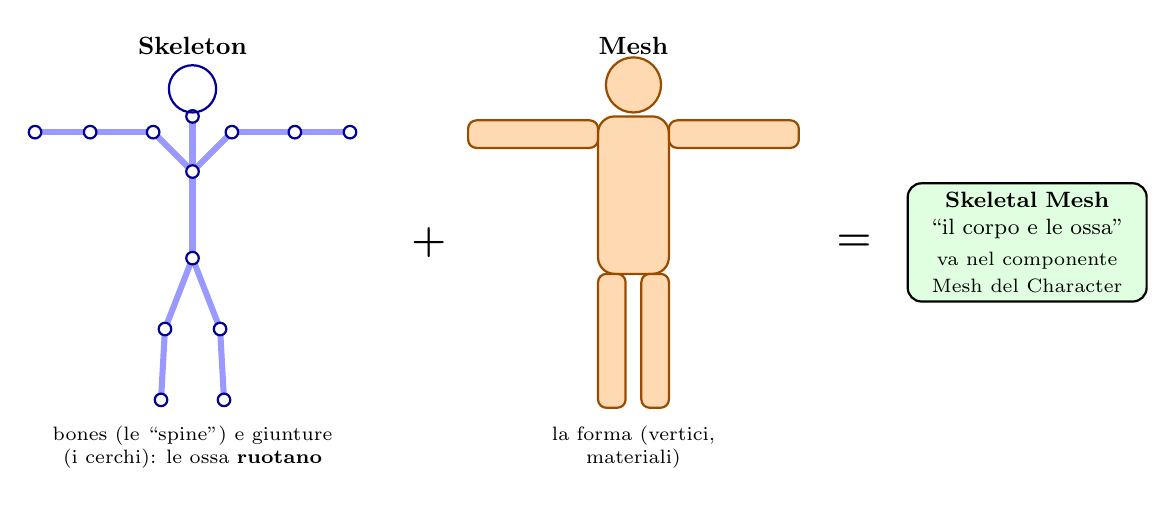
\begin{tikzpicture}[font=\footnotesize,
  ue8bone/.style={draw=blue!60!black, fill=blue!15, thick},
  ue8joint/.style={draw=blue!60!black, fill=white, thick, circle, inner sep=1.6pt}]
  % --- Skeleton (sinistra)
  \node[font=\small\bfseries] at (0,4.3) {Skeleton};
  \coordinate (pel) at (0,1.6); \coordinate (spi) at (0,2.7); \coordinate (nec) at (0,3.4);
  \coordinate (sl) at (-0.5,3.2); \coordinate (sr) at (0.5,3.2);
  \coordinate (el) at (-1.3,3.2); \coordinate (er) at (1.3,3.2);
  \coordinate (hl) at (-2.0,3.2); \coordinate (hr) at (2.0,3.2);
  \coordinate (kl) at (-0.35,0.7); \coordinate (kr) at (0.35,0.7);
  \coordinate (fl) at (-0.4,-0.2); \coordinate (fr) at (0.4,-0.2);
  \foreach \a/\b in {pel/spi, spi/nec, spi/sl, spi/sr, sl/el, sr/er, el/hl, er/hr,
                     pel/kl, pel/kr, kl/fl, kr/fr}
    \draw[ue8bone, line width=2.2pt, blue!40] (\a) -- (\b);
  \foreach \p in {pel, spi, nec, sl, sr, el, er, hl, hr, kl, kr, fl, fr}
    \node[ue8joint] at (\p) {};
  \draw[blue!60!black, thick] (0,3.75) circle (0.3);
  \node[font=\scriptsize, align=center] at (0,-0.8) {bones (le ``spine'') e
    giunture\\(i cerchi): le ossa \textbf{ruotano}};
  % --- piu'
  \node[font=\Large\bfseries] at (3.0,1.8) {+};
  % --- Mesh
  \begin{scope}[xshift=5.6cm]
    \node[font=\small\bfseries] at (0,4.3) {Mesh};
    \fill[orange!30, draw=orange!60!black, thick, rounded corners=6pt]
      (-0.45,1.4) rectangle (0.45,3.4);
    \fill[orange!30, draw=orange!60!black, thick] (0,3.8) circle (0.35);
    \fill[orange!30, draw=orange!60!black, thick, rounded corners=3pt]
      (-2.1,3.0) rectangle (-0.45,3.35);
    \fill[orange!30, draw=orange!60!black, thick, rounded corners=3pt]
      (0.45,3.0) rectangle (2.1,3.35);
    \fill[orange!30, draw=orange!60!black, thick, rounded corners=3pt]
      (-0.45,-0.3) rectangle (-0.1,1.4);
    \fill[orange!30, draw=orange!60!black, thick, rounded corners=3pt]
      (0.1,-0.3) rectangle (0.45,1.4);
    \node[font=\scriptsize, align=center] at (0,-0.8) {la forma (vertici,\\materiali)};
  \end{scope}
  % --- uguale
  \node[font=\Large\bfseries] at (8.4,1.8) {=};
  \node[draw, thick, rounded corners=5pt, fill=green!12, align=center, text width=2.8cm]
    at (10.6,1.8) {\textbf{Skeletal Mesh}\\``il corpo e le ossa''\\[2pt]
    \scriptsize va nel componente Mesh del Character};
\end{tikzpicture}
\caption{Skeletal Mesh e Skeleton secondo la lezione: due asset diversi. Lo Skeleton è
la gerarchia delle ossa, con le giunture; la Skeletal Mesh è la forma legata a quelle
ossa. Le animazioni sono rotazioni delle ossa, e sono legate allo Skeleton. Schema
ricostruito, non in scala.}
\label{ue8:fig:skeletal}
\end{figure}

\paragraph{Approfondimento: perché due asset.} Romero e Sewell (capitolo 17, ``Animation
Blueprints'') spiegano la separazione così: ``uno Skeleton è una gerarchia di ossa
interconnesse, usata per animare i vertici poligonali di una Skeletal Mesh''; e
``siccome l'animazione è fatta sullo Skeleton, può essere condivisa da molte Skeletal
Mesh che usano lo stesso Skeleton''. È il motivo per cui un gioco può avere decine di
personaggi diversi con un solo set di animazioni, e il motivo per cui, più avanti, le
animazioni del manichino di Unreal potranno essere \emph{ritargettate} sul cavaliere di
Mixamo, che ha uno scheletro simile ma non identico. Gli autori elencano anche i cinque
editor che si aprono dagli asset di animazione, con i bottoni in alto a destra già visti
dal docente: \emph{Skeleton Editor}, \emph{Skeletal Mesh Editor}, \emph{Animation
Editor}, \emph{Animation Blueprint Editor} e \emph{Physics Asset Editor}.

% ---------------------------------------------------------------------
\section{Le animazioni di Mixamo}
\label{ue8:sec:mixamoanim}

``Torniamo su Mixamo.'' L'importante è che nella viewport di Mixamo ci sia il proprio
personaggio, ``non un altro''; poi si passa alla categoria \textbf{Animations}. Servono
\textbf{tre animazioni} principali: \textbf{idle}, \textbf{walk} e \textbf{run}. ``La
idle, per chi non lo sapesse, sono le animazioni di stallo'': il personaggio ``sta fermo,
sta respirando'', il \emph{breathing}.

\paragraph{I controlli di Mixamo.} Sulla destra, per ogni animazione, ci sono alcuni
cursori; il docente li prova su animazioni diverse per farli vedere bene:
\begin{itemize}
  \item \textbf{Overdrive}: la velocità dell'animazione. ``Se aumento l'overdrive,
        questa animazione si velocizza sempre di più; se lo diminuisco, sarà
        lentissima'';
  \item \textbf{Character Arm-Space}: su alcuni modelli, la distanza delle braccia dal
        corpo, ``diventa sempre di più oppure diminuisce''. Attenzione al
        \emph{clipping}, le braccia che entrano nel corpo: ``infatti clippa
        malissimo''. Il docente suggerisce valori intorno a 50;
  \item \textbf{Trim}: ``tagliare l'animazione'', prenderne solo un pezzo. Ma ``viene
        fuori malissimo, perché non c'è il ritorno all'idle'': l'animazione tagliata non
        si chiude su sé stessa;
  \item \textbf{Mirror}: presente solo su alcune animazioni, ``semplicemente flippa
        l'animazione'', la \emph{specchia}. Il docente lo mostra con una Capoeira.
\end{itemize}

\paragraph{Root motion e in place.} Il punto più importante. Il docente apre un
\emph{Walking}: ``vedete che il character sta andando dritto, cioè sta percorrendo dello
spazio''. ``Questa tipologia di animazione viene chiamata \textbf{root motion}'': le
animazioni in root motion ``ereditano il movimento già nell'animazione''. L'esempio è
\emph{Dark Souls 3} (``qualcuno ha giocato Dark Souls 3? Perfetto''): alcune armi hanno
abilità speciali, le \emph{weapon art}, e in un video il docente cerca quella della
\emph{Holy Sword} (``questa non è in root motion, perché sta ferma''; ``eccola, questa
qua''): ``quando io la compio, mi sposto nello spazio già nell'animazione''. ``Non sono
io che gli do il movimento quando premo il tasto'': ``metto il piede in avanti, o faccio
l'affondo'', e il personaggio avanza perché lo fa l'animazione. Le animazioni in root
motion ``spesso sono usate per abilità'' di questo tipo.

``In questo caso, però, su Mixamo non dobbiamo avere un'animazione root motion'', perché
``erediteremmo un movimento che non ci interessa''. ``Noi, a livello del nostro gioco su
Unreal, vogliamo che l'animazione si compia, ma quella che si muove è la
\textbf{capsula}'': ``l'animazione segue la capsula''; ``c'è la mesh con l'animazione su
quella capsula, e di conseguenza si crea il movimento, o l'illusione del movimento''.
Quindi si spunta \textbf{In Place}: ``come potete vedere, adesso l'animazione è sul
posto''. ``Se non trovate una spunta In Place, consiglio di cambiare animazione: ce ne
sono tante'' (figura~\ref{ue8:fig:rootmotion}).

\begin{figure}[htbp]
\centering
\begin{tikzpicture}[font=\footnotesize,
  ue8cap/.style={draw=blue!60!black, thick, rounded corners=7pt, minimum width=0.7cm,
                 minimum height=1.6cm},
  ue8arr/.style={-{Stealth[length=2.4mm]}, very thick}]
  % root motion
  \node[font=\small\bfseries, anchor=west] at (-0.6,2.2) {Root motion};
  \node[ue8cap, fill=blue!8] at (0.3,0.9) {};
  \fill[orange!60] (0.3,1.5) circle (0.14);
  \draw[orange!60!black, very thick] (0.3,1.35) -- (0.3,0.75) -- (0.1,0.2);
  \draw[orange!60!black, very thick] (0.3,0.75) -- (0.5,0.2);
  \foreach \x/\o in {1.6/40, 2.9/60, 4.2/100} {
    \fill[orange!\o] (\x,1.5) circle (0.14);
    \draw[orange!\o!black, very thick] (\x,1.35) -- (\x,0.75) -- (\x-0.2,0.2);
    \draw[orange!\o!black, very thick] (\x,0.75) -- (\x+0.25,0.2);
  }
  \draw[ue8arr, orange!70!black] (0.6,-0.2) -- node[below, font=\scriptsize]
    {è l'animazione a spostare la mesh} (4.4,-0.2);
  \node[font=\scriptsize, align=left, text width=4.6cm, anchor=west] at (-0.6,-1.2)
    {la capsula resta indietro: mesh e collisione si separano. Utile per affondi e
    abilità (le weapon art di \emph{Dark Souls 3}), con Enable Root Motion};
  % in place
  \begin{scope}[xshift=7.4cm]
    \node[font=\small\bfseries, anchor=west] at (-0.6,2.2) {In place};
    \foreach \x/\o in {0.3/40, 1.6/60, 2.9/80, 4.2/100} {
      \node[ue8cap, fill=blue!8] at (\x,0.9) {};
      \fill[orange!\o] (\x,1.5) circle (0.14);
      \draw[orange!\o!black, very thick] (\x,1.35) -- (\x,0.75) -- (\x-0.2,0.2);
      \draw[orange!\o!black, very thick] (\x,0.75) -- (\x+0.25,0.2);
    }
    \draw[ue8arr, blue!60!black] (0.6,-0.2) -- node[below, font=\scriptsize]
      {è il Character Movement a spostare la capsula} (4.4,-0.2);
    \node[font=\scriptsize, align=left, text width=4.6cm, anchor=west] at (-0.6,-1.2)
      {l'animazione cammina sul posto, e la mesh segue la capsula: è quello che serve per
      idle, walk e run};
  \end{scope}
\end{tikzpicture}
\caption{Root motion e in place. In un'animazione root motion lo spostamento è dentro
l'animazione; in un'animazione in place il personaggio cammina sul posto, e a muoversi
nel mondo è la capsula del Character. Per la locomozione di base la lezione usa solo
animazioni in place. Schema ricostruito.}
\label{ue8:fig:rootmotion}
\end{figure}

\paragraph{Le impostazioni di download.} Al download Mixamo chiede alcune opzioni
(tabella~\ref{ue8:tab:mixamo}):
\begin{itemize}
  \item \textbf{Format}: \textbf{FBX Binary}, ``ci va bene così'';
  \item \textbf{Frames per Second}: \textbf{30}. ``Le animazioni devono essere allo
        stesso tipo di frame'': ``meglio sempre prenderle tutte quante allo stesso
        numero di frame'', ``perché se no avete dei problemi'', soprattutto ``nel
        \emph{blending}, cioè nel mixare'' due animazioni con frame rate diversi;
  \item \textbf{Skin}: \textbf{Without Skin}. ``La skin è se volete prendere
        l'animazione con il modello: non ci interessa, perché il modello ce l'abbiamo
        già'';
  \item \textbf{Keyframe Reduction}: \textbf{none}, ``non ci interessa'' ridurre i
        keyframe.
\end{itemize}
Il docente scrive in chat le tre animazioni da cercare, ``idle, walk e run/sprint'',
lasciando ``la libertà di scegliere quelle che volete'': ``importante che abbiate
un'animazione che respira, sta fermo, eccetera, una che cammina e una che fa lo
sprint''. Lui ha preso \emph{Idle}, \emph{Walking} e \emph{Slow Run}. ``Vi lascio 5, 10
minuti.''

\begin{table}[htbp]
\centering
\small
\begin{tabular}{@{}p{3.2cm}p{3.6cm}p{7.2cm}@{}}
\toprule
\textbf{Opzione} & \textbf{Valore} & \textbf{Perché} \\
\midrule
\multicolumn{3}{@{}l}{\emph{Personaggio}} \\
Format & FBX Binary & il formato che Unreal importa \\
Pose & T-Pose & la posa di riferimento del rig; togliere l'animazione applicata (la X) \\
\midrule
\multicolumn{3}{@{}l}{\emph{Animazioni (idle, walk, run)}} \\
Format & FBX Binary & come sopra \\
Skin & Without Skin & il modello c'è già: serve solo il movimento delle ossa \\
Frames per Second & 30 & tutte allo stesso frame rate, per non avere problemi nel
blending \\
Keyframe Reduction & none & nessuna riduzione dei keyframe \\
In Place & spuntato & niente root motion: a muoversi è la capsula \\
Overdrive, Arm-Space, Trim, Mirror & a piacere & velocità, distanza delle braccia
(attenzione al clipping), taglio, specchio \\
\bottomrule
\end{tabular}
\caption{Le impostazioni di download di Mixamo indicate a lezione.}
\label{ue8:tab:mixamo}
\end{table}

\paragraph{Approfondimento: Mixamo e Unreal.} Mixamo è un servizio gratuito di Adobe, a
cui si accede con un account Adobe; personaggi e animazioni si possono usare anche in
progetti commerciali. Il suo rig ha una gerarchia simile a quella del manichino di
Unreal (Manny e Quinn), ma i nomi delle ossa sono diversi (le ossa di Mixamo hanno il
prefisso \emph{mixamorig:}), e manca un osso \emph{root} alla base, sotto il bacino.
Per questo le animazioni di Mixamo in root motion non funzionano bene in Unreal senza
correzioni: lo spostamento è registrato sull'osso del bacino (\emph{Hips}) invece che su
un root. Con le animazioni \emph{In Place}, come quelle della lezione, il problema non si
pone. La mancanza dell'osso root e i nomi diversi sono anche il motivo per cui, per usare
sul cavaliere le animazioni del manichino (il salto, la caduta), servirà il
\textbf{retargeting} annunciato dal docente, con gli asset \emph{IK Rig} e \emph{IK
Retargeter} di Unreal Engine 5.

% ---------------------------------------------------------------------
\section{Importare le animazioni sullo scheletro}
\label{ue8:sec:importanim}

Dopo i minuti di scelta (``ci siete tutti, ragazzi? Sì, perfetto'') si importano le
animazioni. I file scaricati hanno il nome dell'animazione (``slow run, walking,
eccetera''); ``l'importante è che ci sia FBX sopra''. Al docente una delle due versioni
di Walking era rotta, e usa \emph{Walking 1}. ``Consiglio: fate meglio una cartella'':
\textbf{Animation}. ``Fatela una per una, vi consiglio.''

\paragraph{Lo scheletro obbligatorio.} La finestra di import è ``praticamente la stessa
schermata'', ``ma differenza sostanziale'': in basso, \textbf{Import} è grigio, non si
può premere. ``Per l'animazione in particolare gli serve uno scheletro a cui adattare
l'animazione.'' Nella sezione \textbf{Common} c'è il campo \textbf{Skeleton}: si apre la
tendina, in cui compaiono ``tutti gli scheletri'', compreso quello del manichino ``che
usiamo per Unreal'', e si sceglie \emph{il proprio}, quello creato dall'import del
personaggio. ``A questo punto, Import vi diventa blu.'' Nella stessa finestra il docente
indica anche la spunta sull'import della sola animazione (nella trascrizione: ``fate sì
che Import Only Animation sia ok''); la frase che segue è confusa.

\paragraph{Targettare.} ``Ecco a voi che si è creata un'animazione.'' ``Il file di per sé
è a parte, però lui ha \textbf{targettato}'' (``prendete questo termine'') ``la nostra
animazione su quello scheletro in particolare''. Un'animazione appartiene a uno
scheletro, e si può usare solo con le mesh di quello scheletro.

\paragraph{Approfondimento: le opzioni di import di un'animazione.} Nella finestra FBX
di Unreal Engine 5, quando il campo \emph{Skeleton} è impostato e la spunta
\emph{Import Mesh} è tolta, Unreal importa \emph{solo} le animazioni contenute nel file,
senza creare un'altra Skeletal Mesh e un altro scheletro; con \emph{Import Animations}
attivo, ogni animazione diventa un asset \textbf{Animation Sequence}. È il caso dei file
di Mixamo scaricati \emph{Without Skin}, che contengono solo le ossa animate. Se invece
si lascia vuoto il campo Skeleton su un file con la mesh, Unreal crea uno scheletro nuovo
a ogni import: è facile ritrovarsi con due scheletri quasi identici (``mi sa che ci sono
due ragazzi che hanno importato due'' scheletri, osserva il docente sulla sua tendina) e
con animazioni non compatibili fra loro.

% ---------------------------------------------------------------------
\section{L'editor dell'animazione}
\label{ue8:sec:animeditor}

Con un doppio clic sull'animazione si apre l'\textbf{Animation Editor}, ``che vi permette
di visualizzare tutte le particolarità della nostra animazione''.

\paragraph{I controlli.} In basso c'è il pannello di controllo: andare al primo o
all'ultimo frame (\emph{To Front}, \emph{To End}), al frame precedente o successivo
(``frame per frame per frame''). ``Le animazioni sono costituite da frame'': questa ne ha
\textbf{30}. Con \textbf{spazio}, o con il pulsante, \emph{Play} e \emph{Pause}.

\paragraph{Asset Details.} Sul lato dell'editor c'è il pannello \textbf{Asset Details}
(``se non vedete una finestra, la potete trovare su Window $\rightarrow$ Asset Details'',
``o Finestra $\rightarrow$ Dettagli dell'asset, suppongo, in italiano''). Ci sono molti
dati ``che nessuno andrebbe a vedere''; le cose principali:
\begin{itemize}
  \item \textbf{Loop}: ``se questa animazione la vogliamo che vada in loop'': ``quando
        finisce, ricomincia'';
  \item \textbf{Rate Scale}: a 1 è la velocità normale; ``se metto 1,5 l'animazione è
        più veloce''; a 2 ancora di più; ``40, diventa un casino''. ``È un po' come
        l'overdrive che abbiamo visto'' su Mixamo;
  \item \textbf{Root Motion}: la spunta \emph{Enable Root Motion} non è attiva, ``va
        bene così'', perché l'animazione è in place.
\end{itemize}
Lo stesso per le altre due animazioni: Idle, Slow Run (``vi chiederà sempre lo
scheletro''). ``Se aprite le vostre animazioni, sono giuste, sono davanti a voi?'' Alla
fine: ``dovreste avere tutte e tre le nostre belle animazioni''.

% ---------------------------------------------------------------------
\section{L'Animation Blueprint}
\label{ue8:sec:abp}

``La domanda sorge spontanea: come facciamo a metterle su un character?'' Con
l'\textbf{Animation Blueprint}.

\paragraph{La creazione.} Nella cartella del personaggio (il docente l'ha chiamata
\textbf{Characters}) si crea una cartella \textbf{Blueprint}. Poi tasto destro,
\textbf{Animation $\rightarrow$ Animation Blueprint}. La finestra chiede ``di quale
scheletro'': si sceglie il proprio (il docente, ``il mio paladino''), \textbf{Create}, e il
nome: \textbf{ABP\_Knight}, con il prefisso ABP per \emph{Animation Blueprint} (``io ho
chiamato Knight, però voi chiamatelo Ciccio Baciccio''). A uno studente che non ha
capito, il docente ripete: ``Animation, Animation Blueprint; vi chiederà lo scheletro;
selezionate lo scheletro vostro''. L'Animation Blueprint ``sarà la logica, quindi la
parte di programmazione'' delle animazioni ``del nostro bellissimo nuovo character''.

\paragraph{L'editor.} ``L'Animation Blueprint è abbastanza pieno di roba'', ``ci si può
confondere facilmente''. Le parti:
\begin{itemize}
  \item a sinistra, la \textbf{preview}, con il cavaliere in T-pose: ``e va benissimo,
        perché è la sua forma base'';
  \item l'\textbf{AnimGraph}, con il blocco \textbf{Output Pose}: ``tutti i calcoli che
        andremo a fare di animazioni'' si collegano a lui, ``e questo blocco ci dice:
        guarda, esce fuori questa roba'';
  \item l'\textbf{Event Graph}, ``come ce l'abbiamo in un classico Blueprint'', dove si
        possono ``creare e prendere variabili, modificare cose''.
\end{itemize}
``Esistono due ambienti particolari'': nel primo, l'AnimGraph, ``si ragiona per quanto
riguarda le animazioni''; nel secondo, l'Event Graph, ``a livello di programmazione''.

\paragraph{I due dati che servono.} Nell'Event Graph si devono ricavare due cose dal
personaggio:
\begin{enumerate}
  \item la \textbf{velocità}, ``perché vogliamo che la nostra animazione di camminata e
        di corsa, o di idle, sia relativa alla velocità che abbiamo al momento col
        character''. ``C'è una comunicazione tra i dati di gioco, quindi il movimento, e
        le animazioni'': ``dato un certo valore di velocità, cambia l'animazione'';
  \item se il personaggio \textbf{sta cadendo} o no, ``in modo da dire: guarda, sto
        saltando, sto iniziando a cadere; fammi un'animazione di salto, e fammi il loop
        del \emph{falling}''.
\end{enumerate}
Le animazioni di salto e caduta ``non le abbiamo importate'': ``le andremo a
ritargettare in seguito'', perché ``Unreal ci mette a disposizione la possibilità di
ritargettare delle animazioni'', ``ma non lo vedremo adesso''.

\paragraph{Event Blueprint Initialize Animation.} Il primo nodo è \textbf{Event Blueprint
Initialize Animation}: ``dice: quando l'animazione inizia''. ``Come abbiamo visto, gli
eventi come il Begin Play vengono fatti quando viene inizializzato tutto'': questo ``è il
Begin Play, ma per le animazioni''. (A questo punto Unreal si blocca di nuovo:
``è crashato Unreal; direi che oggi è proprio una gran roba''. ``Mi sa che mi tocca
svuotare un po' di memoria.'' Liberata la memoria, si riparte.)

\paragraph{Try Get Pawn Owner.} Dall'evento si chiama \textbf{Try Get Pawn Owner}.
``Questo blocco ci permette di comunicare con il nostro Pawn'', ``il nostro player''.
``Immaginatevi due ambienti separati'': nel Gameplay Framework ``il Pawn è quello che
controlla il character'', mentre l'animazione ``è subordinata al Pawn''. ``Quindi andiamo
a dire: ehi, provami a prendere l'owner, cioè il pawn owner.'' Poi ``andiamo a fare un
cast: abbiamo detto BP\_Knight\ldots{} Ah, giusto, ragazzi. Abbiamo scordato una cosa.
Dobbiamo creare effettivamente il nostro character.''

% ---------------------------------------------------------------------
\section{Il nuovo Character: BP\_Knight1}
\label{ue8:sec:character}

``Dobbiamo comunicare con il nostro character, per dire: guarda, mi servono questi dati
del movimento.'' Nella cartella Blueprint del personaggio: \textbf{Blueprint Class}, e
``attenzione'': come genitore si sceglie \textbf{Character}. Il nome:
\textbf{BP\_Knight1}.

\paragraph{I componenti del Character.} ``I character, a differenza degli actor, sono
costituiti di base da'':
\begin{itemize}
  \item un \textbf{Capsule Component}, la capsula;
  \item una \textbf{freccia} (\emph{Arrow}), ``per far capire qual è il forward vector
        della capsula'';
  \item la \textbf{Mesh}, una Skeletal Mesh;
  \item il \textbf{Character Movement}, ``il componente che definisce il movimento del
        character''. Nei suoi Details, in \emph{General Settings}, ci sono la
        \textbf{Gravity Scale}, la \textbf{Max Acceleration}, la \textbf{Braking
        Friction}. ``Come abbiamo detto, dobbiamo interfacciare le animazioni con i
        valori del movimento'', e quei valori stanno qui.
\end{itemize}

\paragraph{La Skeletal Mesh.} Nella Mesh si assegna la Skeletal Mesh del cavaliere (``devo
ricordarmi l'indirizzo''; ``no, non è questo, è questo qua''). Il personaggio ``è apparso
in modo abbastanza scorretto'', fuori posto rispetto alla capsula e girato male: ``basta
riposizionarlo''. ``Consiglio di fare lo \textbf{snapping}'': si abbassa la mesh in modo
che i piedi tocchino il fondo della capsula, e la si ruota ``in direzione della capsule'',
cioè con la faccia nella direzione della freccia (per i personaggi di Mixamo
serve di solito una rotazione di $-$90 gradi sulla Z; il valore esatto la trascrizione
non lo dice). ``Eccovi che abbiamo creato il nostro primo character.
Questa è la T-pose, meraviglioso.''

\paragraph{L'Anim Class.} ``Ma in questo caso non ha ancora animazioni.'' ``Come facciamo
a dire: guarda, devi usare proprio questa Animation Blueprint?'' Nella \textbf{Mesh}, alla
voce \textbf{Anim Class}, la tendina mostra tutti gli Animation Blueprint compatibili:
si sceglie \textbf{ABP\_Knight1} (il nome dell'asset del docente). ``Non è cambiato
niente, ma l'abbiamo messo in comunicazione'': quando l'Animation Blueprint avrà delle
animazioni, ``questo qua si aggiornerà''. La relazione è a due vie: il Character dice
quale Animation Blueprint usare (Anim Class), e l'Animation Blueprint chiede al suo
proprietario i dati (Try Get Pawn Owner).

% ---------------------------------------------------------------------
\section{Initialize: il cast e le referenze}
\label{ue8:sec:initialize}

Tornati nell'Animation Blueprint, il grafo dell'inizializzazione si completa
(figura~\ref{ue8:fig:abpgraph}, in alto):
\begin{enumerate}
  \item \textbf{Event Blueprint Initialize Animation};
  \item \textbf{Try Get Pawn Owner} $\rightarrow$ \textbf{Cast To BP\_Knight1}
        (``castate al vostro character, come l'avete chiamato'');
  \item dal pin As BP Knight1, \textbf{Promote to Variable}: una variabile referenza
        \textbf{BP\_Knight1}. ``Andiamo a creare una referenza del character, in modo
        tale che sia più semplice'': ``ogni volta che dovremmo prendere una cosa del
        character, dovremmo, se no, fare sempre Cast To BP\_Knight'', ed ``appesantisce
        castare sempre un qualcosa. Quindi lo facciamo all'inizio'';
  \item dalla referenza, \textbf{Get Character Movement}, ``per essere anche un po' più
        esaustivi'', e anche questo \textbf{Promote to Variable}: una variabile
        \textbf{MovementComponent}. ``Abbiamo creato già due variabili che ci faranno
        comodo in seguito.''
\end{enumerate}

\paragraph{Approfondimento: lo stesso grafo del modello Third Person.} Il grafo costruito
dal docente ricalca quasi nodo per nodo l'Animation Blueprint del manichino di Unreal
Engine 5 (\emph{ABP\_Manny}, nel modello Third Person): sull'Initialize, Try Get Pawn
Owner, Cast To Character, Set \emph{Character}, Get Character Movement, Set
\emph{MovementComponent}; sull'Update, controllo di validità, poi Set \emph{Velocity},
Set \emph{GroundSpeed} (Vector Length XY), Set \emph{ShouldMove} e Set \emph{IsFalling}.
La differenza è il cast: il modello fa Cast To \emph{Character}, la classe generica,
così che lo stesso Animation Blueprint funzioni con qualsiasi personaggio basato su
Character; la lezione fa Cast To BP\_Knight1, che dà accesso anche alle variabili
aggiunte nel cavaliere (utile, per esempio, per uno sprint), ma lega l'ABP a quella
classe.

% ---------------------------------------------------------------------
\section{Update: la velocità e la caduta}
\label{ue8:sec:update}

\paragraph{Event Blueprint Update Animation.} ``Questo evento avviene quasi come il Tick,
a ogni frame.'' ``Quando un'animazione si aggiorna, qualsiasi micro movimento è un
Update'': ``se abbiamo un idle, comunque è un'animazione; un walk, comunque è
un'animazione; e il run, comunque è un'animazione'', ``quindi sarà sempre attivo''. ``È
per questo che non facciamo il cast qui'': ``se no farebbe ogni volta, ogni frame,
sempre molto pesante''.

\paragraph{Il Validated Get.} ``Dobbiamo vedere se questo character è valido.'' ``Vi
ricordate gli Is Valid? Se in una variabile c'è qualcosa dentro o non c'è.'' C'è ``una
cosa molto interessante'': si trascina nel grafo un \textbf{Get} della variabile
BP\_Knight1, tasto destro, \textbf{Convert to Validated Get}. Il Get ``normale'' prende la
variabile e basta; il Validated Get ``prende la variabile, e mette anche la
particolarità: se lo prendo ed è valido faccio questo, se non è valido faccio
quest'altro''. Ha un ingresso di esecuzione e due uscite, \textbf{Is Valid} e \textbf{Is
Not Valid}: un Get e un Is Valid in un nodo solo. Sull'uscita Is Valid il docente mette
una \textbf{Sequence} (``un Is Valid, Sequence'') per eseguire in ordine le operazioni
che seguono.

\paragraph{GroundSpeed.} ``Fondamentalmente andiamo a prendere il Movement Component'',
la variabile creata nell'Initialize, e da lì \textbf{Get Velocity}: ``la velocità attuale,
a ogni frame, del character movement''. È un vettore; ``ci interessa solamente il
movimento'' sul piano, ``non ci interessa se salta o meno'', ``quello ci interesserà in
altro modo''. Quindi il nodo \textbf{Vector Length XY}: ``la lunghezza del vettore
solamente sugli assi X e Y'', ``se l'asse X è avanti e dietro e l'asse Y è destra e
sinistra''. Il risultato è un \textbf{float}, e diventa, con \textbf{Promote to
Variable}, \textbf{GroundSpeed}: ``una variabile che rappresenta la nostra velocità
attuale''.

\paragraph{IsFalling.} ``Molto importante per sapere quando saltiamo o quando stiamo
cadendo'': dal Movement Component, il nodo \textbf{Is Falling}. ``Ce ne sono due'': uno è
quello del \emph{Nav Movement}; quello giusto ``deve essere blu all'inizio e rosso alla
fine'', cioè con l'ingresso target blu (il Character Movement) e l'uscita rossa (una
booleana). Il valore va in una variabile, \textbf{IsFalling}, aggiornata a ogni frame,
``in modo tale da sapere che movimento fargli fare'' nel ``giro di animazioni''.

\paragraph{Velocity.} ``Per il futuro, per altre cose che ci serviranno'', anche il
vettore della velocità si promuove a variabile: \textbf{Velocity}, ``così almeno ci sono
delle cose che vogliamo interfacciare con la velocità''. ``Adesso abbiamo tirato fuori la
nostra velocità attuale e il fatto se sta cadendo o meno.'' A uno studente il Get
Velocity non compare: è quello che si ottiene dal Movement Component, con il target
giallo e l'uscita gialla (un vettore); cercandolo in fondo alla lista, ``trovato''.

\begin{figure}[htbp]
\centering
\begin{tikzpicture}[font=\footnotesize,
  ue8node/.style={draw, thick, rounded corners=4pt, align=center, fill=gray!8,
                  minimum height=0.8cm, text width=2.0cm},
  ue8ev/.style={ue8node, fill=red!12},
  ue8pure/.style={ue8node, fill=green!10, rounded corners=8pt},
  ue8var/.style={ue8node, fill=blue!10, rounded corners=8pt},
  ue8exec/.style={-{Stealth[length=2.5mm]}, very thick, black!80},
  ue8data/.style={-{Stealth[length=2mm]}, thick, blue!60!black}]
  % Initialize
  \node[font=\small\bfseries, anchor=west] at (-1.2,1.3) {Inizializzazione (una volta)};
  \node[ue8ev, text width=2.3cm] (ini) at (0,0) {\textbf{Event Blueprint Initialize
    Animation}};
  \node[ue8node, fill=blue!10, text width=1.9cm] (cst) at (3.2,0) {\textbf{Cast To}\\
    BP\_Knight1};
  \node[ue8pure] (tgp) at (3.2,-1.6) {\textbf{Try Get}\\\textbf{Pawn Owner}};
  \node[ue8node, text width=2.0cm] (s1) at (6.2,0) {\textbf{Set}\\BP\_Knight1};
  \node[ue8node, text width=2.8cm] (s2) at (9.6,0) {\textbf{Set}\\Movement\-Component};
  \node[ue8pure, text width=2.6cm] (gcm) at (9.6,-1.6) {BP\_Knight1 $\rightarrow$\\
    \textbf{Get Character Movement}};
  \draw[ue8exec] (ini) -- (cst);
  \draw[ue8data] (tgp) -- node[right, font=\scriptsize]{Object} (cst);
  \draw[ue8exec] (cst) -- (s1);
  \draw[ue8exec] (s1) -- (s2);
  \draw[ue8data] (gcm) -- (s2);
  % Update
  \node[font=\small\bfseries, anchor=west] at (-1.2,-3.1) {Aggiornamento (ogni frame)};
  \node[ue8ev, text width=2.3cm] (upd) at (0,-4.6) {\textbf{Event Blueprint Update
    Animation}};
  \node[ue8var, text width=2.0cm] (vg) at (3.3,-4.6) {\textbf{Validated Get}\\
    BP\_Knight1};
  \node[ue8node, text width=1.6cm] (seq) at (6.5,-4.6) {\textbf{Sequence}};
  \node[ue8node, text width=3.6cm, align=left] (sv) at (10.6,-3.4) {\textbf{Set
    Velocity} $\leftarrow$\\MovementComponent $\rightarrow$ Get Velocity};
  \node[ue8node, text width=3.6cm, align=left] (sg) at (10.6,-4.7) {\textbf{Set
    GroundSpeed} $\leftarrow$\\Vector Length XY (Velocity)};
  \node[ue8node, text width=3.6cm, align=left] (sf) at (10.6,-6.0) {\textbf{Set
    IsFalling} $\leftarrow$\\MovementComponent $\rightarrow$ Is Falling};
  \draw[ue8exec] (upd) -- (vg);
  \draw[ue8exec] (vg) -- node[above, font=\scriptsize]{Is Valid} (seq);
  \draw[ue8exec] (seq.east) -- ++(0.4,0) |- node[pos=0.75, above, font=\scriptsize]
    {Then 0} (sv.west);
  \draw[ue8exec] (seq.east) -- ++(0.4,0) |- node[pos=0.75, above, font=\scriptsize]
    {Then 1} (sg.west);
  \draw[ue8exec] (seq.east) -- ++(0.4,0) |- node[pos=0.75, above, font=\scriptsize]
    {Then 2} (sf.west);
\end{tikzpicture}
\caption{I due grafi dell'Event Graph di ABP\_Knight. In alto, una sola volta: si prende
il proprietario, lo si converte nel cavaliere e si salvano due referenze. In basso, a
ogni frame: se la referenza è valida, si aggiornano Velocity (vettore), GroundSpeed (la
sua lunghezza sul piano XY) e IsFalling (booleana). Accanto a ogni Set, il valore che riceve.
Schema ricostruito.}
\label{ue8:fig:abpgraph}
\end{figure}

\paragraph{Un registro di dati.} ``Questo graph funziona letteralmente come'' un
registro (la trascrizione dice ``registri di credito''): serve ``principalmente per
interfacciarsi con il nostro bellissimo character'', e ``ci serve per capire valori,
vedere cose'', ``parliamo di numeri per lo più''. Le animazioni vere si decidono altrove.

\paragraph{Approfondimento: perché l'AnimGraph non legge da solo.} Romero e Sewell
(capitolo 17) descrivono la stessa divisione dei compiti: ``usiamo l'EventGraph di un
Animation Blueprint per prendere i dati dal Pawn o dal Character che sta usando l'istanza
dell'Animation Blueprint, e per aggiornare le variabili dell'Animation Blueprint''; e
``l'AnimGraph può accedere solo alle variabili dell'Animation Blueprint''. Il loro esempio
è più semplice di quello della lezione: sull'Update un Is Valid sul Try Get Pawn Owner,
Get Velocity dal Pawn, \emph{VectorLength} (la lunghezza su tutti e tre gli assi) e Set
di una variabile \emph{Speed}. La scelta del docente, \textbf{Vector Length XY}, è più
precisa per la locomozione: con la lunghezza completa, un personaggio che cade dritto
verso il basso avrebbe una velocità alta e farebbe la corsa a mezz'aria. Gli autori
notano anche che \emph{Event Blueprint Update Animation} ha un parametro \emph{Delta Time
X}, il tempo trascorso dall'ultimo frame, utile per interpolare i valori.

% ---------------------------------------------------------------------
\section{L'AnimGraph, un'anteprima del Blend Space e il personaggio finito}
\label{ue8:sec:animgraph}

``Adesso, ragazzi, vi faccio una spiegazione teorica molto corta, perché capisco che siamo
agli ultimi dieci minuti, anzi sette.'' L'AnimGraph, ``differentemente, lavora per
esempio per \emph{state machine}''.

\paragraph{Un'animazione sull'Output Pose.} Il caso più semplice: nell'\textbf{Asset
Browser} dell'editor (``qua trovate tutte le animazioni che sono compatibili con questo
scheletro'') si prende un'animazione, per esempio \emph{Walking 1}, la si trascina
nell'AnimGraph e si collega ``l'omino'' del nodo all'omino dell'\textbf{Output Pose}. Non
è in loop, ma basta spuntare \textbf{Loop Animation} nei Details del nodo. Compile: nella
preview il cavaliere cammina. ``E possiamo vederlo anche nel nostro character'', perché
l'Anim Class ``ci ha permesso di dirgli: guarda, ehi, hai questo in eredità, hai questo
sotto di te, l'Animation Blueprint''. ``Ma, come potete capire, a noi serve molto di più
rispetto a mettere queste animazioni'' una alla volta.

\paragraph{Il Blend Space 1D.} ``Sicuramente la prossima volta andremo a vedere quelli
che sono chiamati \textbf{Blend Space}. Ve lo faccio vedere velocissimamente.'' Il
docente apre un \textbf{Blend Space 1D} (``una dimensione''), creato sullo scheletro del
cavaliere: un grafico con il personaggio che ``ci permette di mettere insieme varie
animazioni che \emph{blendano} tra di loro'', cioè ``che interpolano tra di loro''.
Nella preview, spostandosi sull'asse: idle, poi walking, poi sprint. ``In questo caso ci
sarà solamente un asse, che noi diremo che sarà la nostra \textbf{GroundSpeed}'', la
velocità ``che definisce il movimento'' (figura~\ref{ue8:fig:blendspace}). ``La prossima
volta vedremo di costruire questa tipologia di asset e collegare tutto quanto.''

\begin{figure}[htbp]
\centering
\begin{tikzpicture}[font=\footnotesize,
  ue8pt/.style={draw=black, fill=white, thick, diamond, inner sep=2.2pt}]
  \draw[-{Stealth[length=2.5mm]}, thick] (0,0) -- (11.2,0) node[right]{GroundSpeed};
  \foreach \x/\v in {0/0, 2.5/150, 5/300, 7.5/450, 10/600}
    \draw (\x,0.1) -- (\x,-0.1) node[below, font=\scriptsize]{\v};
  \node[ue8pt] (i) at (0,0) {}; \node[ue8pt] (w) at (2.5,0) {}; \node[ue8pt] (r) at
    (10,0) {};
  \node[above=6pt of i, font=\scriptsize\bfseries] {Idle};
  \node[above=6pt of w, font=\scriptsize\bfseries] {Walking};
  \node[above=6pt of r, font=\scriptsize\bfseries] {Run / Sprint};
  \fill[green!50!black] (6.25,0) circle (0.12);
  \draw[green!50!black, thick, ->] (6.25,0.9) -- (6.25,0.2);
  \node[green!40!black, font=\scriptsize, align=center] at (6.25,1.3) {valore attuale:
    50\% Walking + 50\% Run};
  \node[font=\scriptsize, align=center, text width=11cm] at (5.5,-1.0) {le animazioni
    sono campioni posti sull'asse; fra due campioni Unreal le mescola in proporzione
    alla distanza};
\end{tikzpicture}
\caption{Un Blend Space 1D come quello mostrato in anteprima: un solo asse, la
GroundSpeed calcolata nell'Event Graph, e tre animazioni poste su di esso. I valori
sull'asse sono un esempio, non quelli del docente. Schema ricostruito.}
\label{ue8:fig:blendspace}
\end{figure}

\paragraph{Il personaggio finito.} Per chiudere, il docente mostra dove arriveranno.
``Io posso cambiare il nostro character da qui'': nei \textbf{World Settings} del livello,
nella Game Mode, alla voce \textbf{Default Pawn Class}, sceglie BP\_Knight. In Play, il
cavaliere si muove con idle, camminata e corsa, e ``gli ho messo addirittura pure lo
sprint''. ``Il salto, questo è ritargettato'': è l'animazione classica di Unreal, portata
sullo scheletro di Mixamo. E la vecchia logica funziona con il nuovo personaggio:
``possiamo fare tutte le interazioni, e addirittura la nostra torretta ci segue''.
``Questo lo faremo la prossima volta'', ``perché ci vuole un pochino di continuità''.

\paragraph{Approfondimento: dalle animazioni singole alla State Machine.} Il capitolo 17
di Romero e Sewell mostra i passi successivi, quelli annunciati per la prossima lezione.
Un \textbf{Blend Space} è ``un tipo di asset che permette di mescolare animazioni in base
ai valori di uno o due parametri'': nel loro esempio del modello Third Person (UE4), il
Blend Space di locomozione pone \emph{Idle} a 0, \emph{Walk} a 93,75 e \emph{Run} a 375,
e con una velocità di circa 234 l'animazione risultante è metà camminata e metà corsa.
Trascinato nell'AnimGraph, il Blend Space diventa un nodo \emph{Blendspace Player} con un
ingresso per il parametro, a cui si collega la variabile della velocità; nell'\emph{Anim
Preview Editor} si può cambiare il valore e vedere il risultato senza andare in Play.
Poi la \textbf{State Machine}: un nodo dell'AnimGraph che organizza le animazioni in
\emph{stati} (per esempio \emph{Idle} e \emph{Moving}, e più avanti \emph{Jump} e
\emph{Fall}), collegati da \emph{transizioni} con regole booleane (per esempio
``GroundSpeed $>$ 3'' per passare da fermo a in movimento, o ``IsFalling'' per passare
al salto). È lì che la variabile IsFalling di oggi troverà il suo uso.

% ---------------------------------------------------------------------
\section{I materiali mancanti e la chiusura}
\label{ue8:sec:chiusura}

``Ci sono domande, ragazzi?'' Una studentessa: ``il mio personaggio non c'ha un
materiale, ha solo le texture''. ``Anche il mio non è importato'', aggiunge un altro.

\paragraph{Creare il materiale a mano.} La studentessa condivide lo schermo: il suo
personaggio di Mixamo è un'arciera (\emph{Erika Archer}, a giudicare dalla trascrizione).
``Se non hai un materiale, dovresti crearlo da zero'':
\begin{enumerate}
  \item tasto destro $\rightarrow$ \textbf{Material}, chiamato \textbf{M\_Archer};
  \item aperto il materiale in una finestra piccola, si trascinano dentro tutte le
        \textbf{texture} (``quelle con il label rosso''), che diventano nodi
        \textbf{Texture Sample};
  \item si legge bene il nome di ognuna: la \textbf{Diffuse} va nel \textbf{Base Color}
        (``acciaccala in Base Color''); la \textbf{Normal} va nel \textbf{Normal}.
\end{enumerate}
Leggendo i nomi, però, si scopre che le texture sono di due gruppi: una Diffuse dei
\emph{vestiti} e una della \emph{pelle} (e una delle ciglia, l'\emph{eyelash}). ``Ha due
materiali diversi, forse.'' ``Quindi mi sa che devi fare due materiali: uno per i
vestiti, e l'altro per la pelle'', per esempio \emph{M\_ArcherClothing}.

\paragraph{Gli slot dei materiali.} Per sapere dove va cosa, si apre la Skeletal Mesh:
nei Details, la sezione dei materiali mostra gli slot, con il \textbf{WorldGridMaterial}
(la griglia grigia di default) dove manca un materiale. Gli slot sono \emph{quattro}, non
due. Si mette il nuovo materiale nell'\textbf{Element 0} e si guarda ``dove te lo mette sul
corpo'': passando sopra uno slot, la parte corrispondente si illumina
(\emph{highlight}). Element 0 è il \emph{clothing}; il 2 e il 3 saranno la pelle, con un
altro materiale. ``Tanto, se non avete i materiali ma avete le texture, ragazzi, potete
farlo direttamente a mano.''

\paragraph{Le texture che non ci sono.} A un altro studente non sono state importate
nemmeno le texture. Il docente prova a riprodurre il problema: torna su Mixamo (``Mixamo
non mi risponde più, ottimo''), scarica lo stesso personaggio, \emph{The Boss}
(``use this character''; ``madonna mia''), in T-pose, e lo importa. Nella finestra di
import, nella sezione dei materiali, \textbf{Import Materials} e \textbf{Import
Textures} devono essere attivi (``fai sì che i materiali siano importati''); \emph{Import
Morph Targets} e simili ``non ci interessano''. ``A me importa tutto.'' ``Se c'hai
difficoltà, magari puoi semplicemente riprovare a fare l'import.'' Intanto Federico ha
risolto da solo, assegnando i materiali agli slot con l'highlight: ``allora vuol dire che
ti sei risolto la vita da solo. Perfetto.''

\paragraph{Approfondimento: Diffuse, Normal e gli altri canali.} Una \textbf{Diffuse} (o
\emph{Albedo}, o \emph{Base Color}) è il colore della superficie senza luci né ombre, e
va nel pin Base Color; una \textbf{Normal map}, riconoscibile dal colore azzurro-violetto,
simula i rilievi e va nel pin Normal (Unreal la riconosce all'import e imposta la
compressione \emph{Normalmap}). Se ci sono texture di \emph{Specular}, \emph{Roughness} o
\emph{Gloss}, vanno nei pin corrispondenti, ricordando che una Gloss è l'inverso di una
Roughness (serve un nodo \emph{1-x}, \emph{OneMinus}). Per le ciglia e i capelli, fatti
di piani con trasparenze, il materiale va impostato con \emph{Blend Mode} \emph{Masked}
e l'alfa della texture collegata all'\emph{Opacity Mask}: altrimenti le ciglia appaiono
come rettangoli pieni. Sono gli stessi nodi visti nella terza lezione, dedicata a
texture e materiali.

\paragraph{La chiusura.} ``Altri problemi? Se no, ci sentiamo la prossima volta.''
``Se dovete dichiarare qualcosa, non alla dogana, spero, ci sentiamo su Discord'':
``mandatemi quello che volete, se provate cose''. A Filippo: ``poi magari ti guardo un po'
quelle cosette che abbiamo visto prima''. ``Allora, ragazzi, buona cena, buona serata.
Ci vediamo giovedì. Ciao, ciao.''

\begin{table}[htbp]
\centering
\small
\begin{tabular}{@{}p{5.4cm}p{8.6cm}@{}}
\toprule
\textbf{Sintomo} & \textbf{Causa e rimedio} \\
\midrule
Una variabile ``non si muove'' & creata di nuovo e rimasta al default (0): controllare i
valori; variabili con nomi chiari \\
Errore sull'Audio Component ``non valido'' (Set Pitch Multiplier), solo arrivando in
fondo & caso rimasto aperto; ipotesi: lo Stop distrugge il suono (Auto Destroy) e la
variabile resta a puntare al vuoto. Is Valid, o Auto Destroy disattivato, o reset del Do
Once \\
L'ascensore va sempre più giù e non risale & attivazioni ripetute: booleana Activated
(Branch sul False all'inizio di Activation, false sul Begin Overlap) \\
Il progetto non si apre (si apre solo Unreal) & probabile chiavetta USB staccata male:
rimuoverla in sicurezza; usare un sistema di versione (Git) \\
Il personaggio si ferma un istante sul collezionabile & doppia collisione: mesh in
NoCollision, resta la Sphere Collision \\
On Component Begin Overlap non compare & è selezionata la mesh e non la Collision \\
Get Collectables non compare da Get Game Instance & manca il Cast To GI\_Platform: la
referenza è generica \\
Il cast non funziona & Get Game Instance non collegato all'Object del cast \\
``Non eredita da istanza di gioco''; la classe non compare nei Project Settings & la
Game Instance è stata creata con un altro genitore: ricrearla da GameInstance, sceglierla
in Game Instance Class, rifare variabile e cast \\
Il collezionabile conta ma l'esecuzione si ferma & il filo di esecuzione non passa per
il cast \\
Open Level non carica il livello & nome scritto male: è case sensitive. Copiarlo con F2,
Ctrl+C, Ctrl+V \\
Le palline raccolte riappaiono & normale: il livello viene ricaricato. Salvare lo stato
nella Game Instance (esercizio futuro) \\
Mettere a terra un componente nel Blueprint & nessuna scorciatoia (End vale solo nel
livello): regolare la Z a mano \\
Errore su Set Play Rate all'uscita dal Play & una vecchia referenza alla timeline con lo
stesso nome: eliminarla e usare quella giusta \\
Unreal si chiude durante l'import & memoria video esaurita: liberare memoria e spazio su
disco, reimportare \\
Il personaggio importato è ruotato & Offset Rotation non a zero: controllare Offset
Translation e Rotation all'import \\
Import grigio per un'animazione & manca lo Skeleton: sceglierlo in Common
$\rightarrow$ Skeleton \\
L'animazione sposta il personaggio da sola & è in root motion: riscaricarla da Mixamo
con In Place \\
Get Velocity non compare & cercarlo dal Movement Component (target e uscita gialli) \\
Il personaggio di Mixamo è grigio, senza materiale & creare i materiali a mano (Diffuse
in Base Color, Normal in Normal) e assegnarli agli slot; o reimportare con Import
Materials e Import Textures \\
\bottomrule
\end{tabular}
\caption{I problemi incontrati durante la lezione, con la causa e il rimedio.}
\label{ue8:tab:errori}
\end{table}

\begin{table}[htbp]
\centering
\small
\begin{tabular}{@{}p{4.6cm}p{9.4cm}@{}}
\toprule
\textbf{Nodo, asset o impostazione} & \textbf{Che cosa fa} \\
\midrule
Game Instance (Blueprint Class) & l'oggetto che vive per tutto il gioco; contiene dati
globali \\
Project Settings $\rightarrow$ Maps \& Modes $\rightarrow$ Game Instance Class & sceglie
la Game Instance del progetto \\
Get Game Instance & restituisce la Game Instance, come referenza generica \\
Cast To (classe) & converte una referenza nel tipo specifico; Cast Failed se non lo è \\
Increment Int (++) / Decrement Int ($--$) & aggiunge o toglie 1 a una variabile intera \\
Collision Presets: NoCollision & toglie ogni collisione a un componente \\
Sphere Collision, Sphere Radius & volume sferico e il suo raggio \\
Destroy Actor & distrugge l'actor \\
Evento Key (E) & scatta alla pressione di un tasto (Pressed, Released) \\
Text Render & un testo nel mondo 3D \\
Hidden in Game & nasconde un componente in gioco; tolto, la box si vede \\
Open Level (by Name) & carica un livello dal nome (case sensitive) \\
File $\rightarrow$ New Level (Basic) & un livello con cielo, luce e pavimento \\
Skeletal Mesh / Skeleton / Physics Asset & la mesh con le ossa; la gerarchia delle ossa;
i corpi fisici \\
Offset Translation / Rotation (import) & posizione e rotazione dell'asset rispetto al
pivot \\
Animation Sequence: Loop, Rate Scale, Enable Root Motion & ripetizione, velocità,
movimento dentro l'animazione \\
Animation Blueprint (ABP) & la logica delle animazioni di uno scheletro: Event Graph e
AnimGraph \\
Anim Class (Mesh del Character) & l'Animation Blueprint usato dalla mesh \\
Character (Capsule, Arrow, Mesh, Character Movement) & il Pawn che cammina, salta,
nuota, vola \\
Event Blueprint Initialize Animation & il ``Begin Play'' dell'Animation Blueprint \\
Try Get Pawn Owner & il Pawn che usa l'Animation Blueprint \\
Event Blueprint Update Animation & scatta a ogni aggiornamento dell'animazione, come il
Tick \\
Convert to Validated Get & un Get con le uscite Is Valid e Is Not Valid \\
Sequence & esegue più uscite in ordine \\
Get Velocity / Vector Length XY & la velocità; la sua lunghezza sul piano \\
Is Falling (Character Movement) & vero se il personaggio è in aria \\
Output Pose (AnimGraph) & la posa finale applicata alla mesh \\
Blend Space 1D & mescola animazioni lungo un asse (GroundSpeed) \\
World Settings $\rightarrow$ Default Pawn Class & il personaggio del giocatore in quel
livello \\
\bottomrule
\end{tabular}
\caption{I nodi, gli asset e le impostazioni dell'ottava lezione.}
\label{ue8:tab:nodi}
\end{table}

% ---------------------------------------------------------------------
\section*{Punti chiave del capitolo}
\addcontentsline{toc}{section}{Punti chiave del capitolo}

\begin{itemize}
  \item Il \textbf{Gameplay Framework} è la gerarchia delle entità che Unreal crea mentre
        il gioco gira: \textbf{Game Instance} (per tutta la durata del gioco), livello,
        \textbf{Game Mode} (le regole), \textbf{Game State} e \textbf{Player State} (lo
        stato, condiviso in rete), \textbf{Player Controller} (il ``cervello'' non
        fisico), \textbf{Pawn} e \textbf{Character} (il ``corpo''), e infine l'input.
  \item \textbf{Pubblica non vuol dire globale}: le variabili degli actor muoiono con il
        livello. Per conservare dati fra i livelli si usa la \textbf{Game Instance},
        creata come Blueprint Class da GameInstance e scelta in \textbf{Project Settings
        $\rightarrow$ Maps \& Modes $\rightarrow$ Game Instance Class}. Non va
        appesantita, perché resta in memoria per tutta la partita.
  \item \textbf{Get Game Instance} restituisce una referenza generica, ``la scocca'':
        per leggere le nostre variabili serve il \textbf{Cast To} della nostra classe,
        ``l'abito giusto'' per entrare alla festa. Cast Failed non è un errore, è una
        risposta.
  \item Un \textbf{collezionabile}: Sphere Collision, mesh in \textbf{NoCollision} (niente
        doppia collisione), controllo sul player, \textbf{Increment Int} sulla variabile
        della Game Instance, \textbf{Destroy Actor}.
  \item Un volume che cambia livello: \textbf{Open Level (by Name)} con il nome promosso
        a variabile pubblica. I nomi sono \textbf{case sensitive}: copiarli con F2 e
        Ctrl+C. I livelli nuovi da \textbf{File $\rightarrow$ New Level $\rightarrow$
        Basic}, salvati subito con Ctrl+S.
  \item Una booleana \textbf{Activated} con un Branch fa da cancello: l'ascensore
        ignora le attivazioni ripetute finché il player non lo fa risalire.
  \item Una \textbf{Skeletal Mesh} è ``il corpo e le ossa''; lo \textbf{Skeleton} è un
        asset separato, a cui sono legate le animazioni. Le ossa si \textbf{ruotano},
        non si spostano.
  \item Da \textbf{Mixamo}: personaggio in \textbf{T-pose}, \textbf{FBX Binary};
        animazioni idle, walk e run \textbf{In Place} (non root motion: a muoversi è la
        capsula), \textbf{Without Skin}, \textbf{30 fps} per tutte, nessuna riduzione dei
        keyframe. All'import si controllano gli \textbf{Offset}; le animazioni si
        importano scegliendo lo \textbf{Skeleton}.
  \item L'\textbf{Animation Blueprint} ha due grafi: l'\textbf{Event Graph} raccoglie i
        dati dal personaggio, l'\textbf{Anim\-Graph} decide la posa (\textbf{Output
        Pose}). Il Character lo usa tramite l'\textbf{Anim Class} della Mesh.
  \item Nell'\textbf{Initialize}: Try Get Pawn Owner, Cast To del personaggio, e le
        referenze salvate in variabili (il cast una volta sola). Nell'\textbf{Update},
        che gira a ogni frame: \textbf{Validated Get}, poi \textbf{GroundSpeed} (Vector
        Length XY della Get Velocity), \textbf{IsFalling} e \textbf{Velocity}.
  \item Prossimi passi: il \textbf{Blend Space 1D} sulla GroundSpeed, la State Machine,
        il \textbf{retargeting} del salto, e il personaggio impostato come
        \textbf{Default Pawn Class}.
\end{itemize}

%
%  Tutte le etichette di questo capitolo hanno il prefisso "ue8:"
%  (ue8:cap:..., ue8:sec:..., ue8:fig:..., ue8:tab:...), e tutti gli
%  stili TikZ hanno il prefisso "ue8" (ue8node, ue8exec, ue8data, ...)
%  per non collidere con chiavi native di TikZ né con quelli delle
%  lezioni precedenti. Il capitolo è autonomo: non contiene \ref verso
%  altri capitoli (i rimandi alle lezioni precedenti sono a parole).
%  Le figure sono ricostruzioni schematiche di quanto mostrato e detto a
%  lezione, non copie delle slide o delle schermate del docente. Dove la
%  trascrizione è troppo rovinata per ricostruire un dettaglio, il
%  capitolo lo dice invece di inventarlo.
% =====================================================================

\chapter[Game Instance, livelli e animazioni]{Game Instance, livelli e animazioni: il
Gameplay Framework e un nuovo personaggio}
\label{ue8:cap:gameinstance}

Questa è l'\textbf{ottava lezione} del corso breve di \textbf{introduzione a Unreal
Engine}. Nelle sette lezioni precedenti tutto è avvenuto dentro un solo livello e con un
solo personaggio, il manichino del modello Third Person: la torretta, i proiettili, la
piattaforma che sale, il pulsante che attiva le luci. Oggi la lezione allarga lo sguardo
in due direzioni. La prima è \textbf{uscire dal livello}: cambiare mappa senza perdere
quello che il giocatore ha fatto, cioè \textbf{salvare dei valori in modo globale}. La
seconda è \textbf{cambiare personaggio}: prendere un modello nuovo da \textbf{Mixamo},
importarlo con il suo scheletro e le sue animazioni, e cominciare a costruire la logica
che decide quale animazione mostrare, l'\textbf{Animation Blueprint}.

Il filo che tiene insieme le due parti è il \textbf{Gameplay Framework} di Unreal: la
``gerarchia'' delle entità che l'engine crea e tiene in vita mentre il gioco gira. La
\textbf{Game Instance}, la prima a nascere e l'ultima a morire, è il posto giusto per i
dati che devono sopravvivere al cambio di livello; il \textbf{Pawn} e il
\textbf{Character}, con il loro \textbf{Character Movement}, sono la fonte dei dati
(velocità, caduta) che l'Animation Blueprint legge per animare lo scheletro. ``Andremo
sia a vedere quelle che sono le animazioni e come si gestiscono, ma sia a vedere un po'
quello che è chiamato il \emph{gameplay framework} di Unreal.''

La lezione è \textbf{online}, su Zoom, come le precedenti, ma con una particolarità: la
webcam del docente si rifiuta di funzionare per tutta la serata (``oggi mi vedrete con
uno schermo nero, o almeno il mio schermo è più importante della mia faccia''), e in
due occasioni l'editor si chiude da solo per mancanza di memoria video. Si apre con un
problema di uno studente rimandato alla pausa, prosegue con una parte teorica in slide
sul Gameplay Framework e con la costruzione dei collezionabili, della Game Instance e
dei volumi che cambiano livello; la pausa arriva verso le 17:26, con ripresa alle ``55,
18, solito orario''; la seconda parte è dedicata all'import del personaggio e delle
animazioni e all'Animation Blueprint. Il docente stesso avverte che non si arriverà in
fondo: ``probabilmente questa lezione la riporteremo nella prossima'', in cui si vedranno
i Blend Space e il resto delle animazioni. Si chiude con un ``ci vediamo giovedì''.

Tre avvertenze di lettura, le stesse delle lezioni precedenti. La prima: la
trascrizione è automatica e storpia moltissimi nomi. Unreal è ``Arena Engine'',
``Arreal'', ``a Real'', ``a RIAL'', ``Arial'' e ``Irium'' (quest'ultimo, forse, è il
programma della webcam); la \textbf{Game Instance} è ``View Instance'', ``getViewInstance''
e ``key instance''; \textbf{GI\_Platform} è ``GI Gaming Instance'', ``gi i platform'',
``asg.platform'', ``giiPatform'' e ``Di Alto''; il \textbf{Pawn} è ``Pwn'', ``la Bone'' e
``player born''; \textbf{Get Player Pawn} è ``getLayerOne'' e ``PlayerOh''; il
\textbf{Cast To} è ``castagna''; l'\textbf{On Component Begin Overlap} è ``component
baking per l'acqua'', ``onBegin onComponent onBegin overlap'' e ``On Collision Beginner
per l'app''; il \textbf{Destroy Actor} è ``destroy hardware''; il \textbf{Text Render} è
``text rendere''; la \textbf{Skeletal Mesh} è ``scheletal mesh'' e ``scheda del Mesh''; il
\textbf{Control Rig} è ``control righe''; l'\textbf{Idle} è ``Idol''; il \textbf{root
motion} è ``root in''; la \textbf{T-pose} è ``Tico'', ``tifoso'' e ``Bix ti pose'';
\textbf{FBX Binary} è ``Fibix binary''; il \textbf{Knight} è ``Night''; il \textbf{Try Get
Pawn Owner} è ``try get one''; l'\textbf{Event Blueprint Update Animation} è ``event
blueprint a data animation''; \textbf{IsFalling} è ``isPalling''; il \textbf{Diffuse} è
``Diffuse'', ma l'\textbf{eyelash} è ``ailash''; \textbf{Mixamo} è a volte
``Mixamon''. Dove la ricostruzione è sicura il capitolo usa la forma corretta; dove non
lo è riporta la forma della trascrizione e lo dice. La seconda: all'inizio della
registrazione, durante la pausa e durante i minuti lasciati per scegliere le animazioni
il riconoscimento vocale produce lunghi blocchi di testo senza senso e ripetuto
(``grazie a tutti per l'attenzione che ci ha spiegato'', ``qual è la risposta che ci può
essere?'', ``la situazione è questa, la migliore dal 2005'', ``i genitori a bordo'', la
``dottrina sul mercato del lavoro'', un Vittorio Prodi chiamato in causa senza
motivo, una lunghissima fila di ``non, non, non''): sono artefatti, non parole di nessuno,
e il capitolo li ignora. La terza: gran parte della lezione è una dimostrazione dal vivo
nell'editor, costruita a voce (``tirate fuori'', ``castate'', ``promote to variable''),
e in un paio di punti il docente improvvisa o si accorge di aver saltato un passaggio
(``ah, giusto, ragazzi, abbiamo scordato una cosa''). Il capitolo ricostruisce i grafi da
ciò che il docente dice mentre li costruisce, e li completa, dove serve, con i nomi
esatti dei nodi e dei pin di Unreal Engine 5; dove la trascrizione lascia un buco, lo
dichiara.

\paragraph{Come leggere questo capitolo.} Il capitolo segue l'ordine della lezione. Le
figure ricostruiscono la gerarchia del Gameplay Framework, la vita della Game Instance
attraverso i cambi di livello, il cast come ``abito giusto'', i grafi del collezionabile,
del tasto E e dei due volumi, la differenza fra Skeletal Mesh e Skeleton, quella fra
animazione in root motion e in place, i due grafi dell'Animation Blueprint e il Blend
Space 1D. Le tabelle riassumono le entità del framework, le impostazioni di download di
Mixamo, gli asset creati dall'import, gli errori incontrati dagli studenti e i nodi della
giornata. Qua e là, dei paragrafi di \textbf{approfondimento} collegano la lezione ai
libri di Marcos Romero e Brenden Sewell (\emph{Blueprints Visual Scripting for Unreal
Engine 5} e la seconda edizione dello stesso testo, scritta per Unreal Engine 4), i
testi di riferimento per questa parte del libro, e a qualche nozione tecnica generale su
Unreal Engine 5; sono segnalati come tali e non fanno parte della lezione.

Il percorso del capitolo:
\begin{enumerate}
  \item l'\textbf{inizio della lezione}: un errore sul suono della piattaforma, Mixamo e
        le Game Jam (sezione~\ref{ue8:sec:inizio});
  \item il \textbf{programma}, le \textbf{variabili globali} e la dimostrazione dei
        collezionabili che passano da un livello all'altro (sezioni
        \ref{ue8:sec:programma} e~\ref{ue8:sec:demo});
  \item il \textbf{Gameplay Framework} di Unreal, dalla Game Instance all'input
        (sezione~\ref{ue8:sec:framework});
  \item il \textbf{fix dell'ascensore} con la booleana Activated
        (sezione~\ref{ue8:sec:ascensore});
  \item la \textbf{Game Instance}: creazione, variabile, Project Settings
        (sezione~\ref{ue8:sec:gi});
  \item il \textbf{collezionabile}, il \textbf{cast} e il tasto E (sezioni
        da~\ref{ue8:sec:collectible} a~\ref{ue8:sec:tastoe});
  \item i due \textbf{volumi}: lo shop che azzera e il volume che \textbf{carica un
        livello} (sezioni da~\ref{ue8:sec:shop} a~\ref{ue8:sec:prova});
  \item \textbf{Mixamo}, la pausa e i problemi degli studenti (sezioni
        \ref{ue8:sec:mixamochar} e~\ref{ue8:sec:pausa});
  \item l'\textbf{import} del personaggio, lo \textbf{scheletro} e le
        \textbf{animazioni} di Mixamo (sezioni da~\ref{ue8:sec:import}
        a~\ref{ue8:sec:animeditor});
  \item l'\textbf{Animation Blueprint}, il nuovo \textbf{Character} e l'AnimGraph
        (sezioni da~\ref{ue8:sec:abp} a~\ref{ue8:sec:animgraph});
  \item i \textbf{materiali} mancanti e la chiusura (sezione~\ref{ue8:sec:chiusura}).
\end{enumerate}

% ---------------------------------------------------------------------
\section{Prima della lezione: l'Audio Component, Mixamo e le Game Jam}
\label{ue8:sec:inizio}

La registrazione comincia con i saluti (``buonasera, buonasera, buonasera'') e con le
scuse del docente: ``scusate, ragazzi, se non mi faccio vedere, ma a quanto pare ho dei
problemi con la webcam''. Il sospetto è un conflitto con OBS, il programma di
registrazione (``forse OBS potrebbe fare contrasto''); i tentativi si ripetono per tutta
la prima parte, senza successo. ``Non vi preoccupate: vi guardo, mi ascoltate, ma non mi
vedete.''

\paragraph{Le variabili chiare.} ``Come state, ragazzi? Avete un po' sperimentato?''
Uno studente ha recuperato dalla registrazione la lezione del giovedì precedente, e
racconta il suo unico problema: ``non funzionava perché nella variabile non avevo messo
il tempo, e quindi non si muoveva niente''. Il docente ne fa una regola: ``il fatto di
avere delle variabili chiare e concise ti finisce proprio il lavoro'', perché altrimenti
``stai sempre là a riguardarle'' chiedendoti ``ma perché non si muove?'', finché non ti
ricordi ``che l'hai creata di nuovo, però sta a zero''. Una variabile appena creata ha
il suo valore di default (zero, per i numeri), e un tempo, una durata o una velocità
lasciati a zero fermano tutto senza dare errori.

\paragraph{Mixamo e le Game Jam.} Uno studente chiede se il sito condiviso su Discord sia
gratuito: ``sì, sì, assolutamente, non ci avete niente da spendere''. È
\textbf{Mixamo}, ``un'ottima risorsa'' che oggi verrà usata ``in modo attivo'': essendo
uno strumento di Adobe ``abbastanza preciso nel replicare le animazioni'', e avendo
modelli ``abbastanza compatibili'' con quelli di Unreal, permette di avere personaggi e
animazioni senza animarli a mano. ``Ci sono animazioni migliori, perché esistono i pack
che si pagano fior di quattrini'', ma per cominciare Mixamo è ``il ben di Dio''. Il
docente lo usa soprattutto per le \textbf{Game Jam}: ``uno ha mai fatto una Game Jam?''
Gli studenti rispondono da soli: ``sono gli eventi dove si programma un videogioco in
pochi giorni''. ``Fondamentalmente si programma il gioco in pochi giorni, che va dai tre
giorni a una settimana'', ``poi ognuno fa un po' come gli pare''; e in quei pochi giorni,
avere animazioni pronte è ciò che fa la differenza.

\paragraph{Il primo problema: l'Audio Component che non è valido.} Filippo condivide lo
schermo. La piattaforma della lezione precedente (``quando ho fatto il bottone, l'altra
volta'') funziona, il suono si sente, ``ma poi mi dà errore'', sul \textbf{Set Pitch
Multiplier}. Il docente insegna prima un'abitudine: nel log degli errori, quando un nome
è sottolineato, ``puoi direttamente cliccare: dice proprio l'errore e ti ci porta''. Il
messaggio, in italiano, è un tentativo di accesso a un componente ``tramite la proprietà
SoundPlatform'' che ``non è valida'': ``vuol dire che l'Audio Component non è stato
spawnato o non esiste''. L'errore compare solo salendo sulla piattaforma, e solo una
volta per partita: ``lo fa solo una volta, fortunatamente'', perché ``quelle successive te
lo fa''. È, a prima vista, lo stesso caso della settima lezione (il pitch impostato prima
che il suono esista), già incontrato con un'altra studentessa.

Il docente prova un rimedio rapido: togliere i due \emph{Get} di SoundPlatform (``questi
due cilindroni'') e collegare i due Set Pitch Multiplier direttamente all'uscita del
\emph{Set} della variabile, ``così dovremmo averci la sicurezza''. Non basta: rileggendo
l'errore, il problema ``non è SoundPlatform, è l'Audio Component'' a non essere valido.
``Visto che è una cosa che ci vuole un attimino di fuori programma'', il caso viene
rimandato alla pausa (sezione~\ref{ue8:sec:pausa}): ``può essere un errore di logica di
base, poi magari sono micro cose''.

\paragraph{Approfondimento: quando l'errore compare una volta sola.} Un errore di tipo
``Accessed None'' (``accesso nullo'', ``non è valida'') che compare \emph{solo la prima
volta} è quasi sempre un problema di \textbf{ordine}: un nodo legge una variabile
referenza prima che qualcuno l'abbia riempita. Dalla seconda volta in poi la variabile
contiene il suono spawnato la volta precedente, e tutto sembra funzionare. Un errore che
compare \emph{solo arrivando in fondo} (come dirà lo studente in pausa) indica invece che
il componente esisteva ma è stato distrutto: un Sound spawnato con \textbf{Spawn Sound at
Location} ha di default l'opzione \emph{Auto Destroy} attiva, cioè l'Audio Component si
distrugge da solo quando il suono finisce o viene fermato con \textbf{Stop}, e la
variabile rimane a puntare a un oggetto non più valido. In entrambi i casi la protezione
è la stessa: un \textbf{Is Valid} prima di usare la referenza, oppure ricreare il suono
quando serve.

% ---------------------------------------------------------------------
\section{Il programma della giornata e le variabili globali}
\label{ue8:sec:programma}

``Oggi andremo a vedere un po' di particolarità.'' Il programma ha due parti:
\begin{itemize}
  \item le \textbf{animazioni}, ``e come si gestiscono'';
  \item il \textbf{Gameplay Framework} di Unreal: il fatto che l'engine, ``nella sua
        esecuzione'', ha ``una gerarchia di quello che tiene, di quello che ha'', cioè
        di entità che ``sono sempre presenti in alcuni momenti''. Fra queste c'è la
        \textbf{Game Instance}, che oggi permetterà ``di salvare dei valori in modo
        globale, chiamiamolo così''.
\end{itemize}

\paragraph{Variabile globale e variabile locale.} ``Non so se qualcuno di voi, a livello
di programmazione, sa cosa si intende con una variabile globale'' (``Federico già lo vedo
bello arzillo''). Una \textbf{variabile globale} è ``visibile in tutte le parti del
codice'': ``indipendentemente dall'ambiente in cui ci troviamo'', nel character, in un
altro oggetto, nel livello, ``è possibile visualizzarla, prenderla, modificarla''.
L'esempio opposto è a portata di mano: la variabile \textbf{ActivableItems} del pulsante
della settima lezione. ``Questa è pubblica'', con l'occhietto aperto, ``la possiamo
vedere da viewport''; ma è pubblica solo nel senso che la si modifica nei Details
dell'istanza. Esiste \emph{dentro} quel pulsante, dentro quel livello: ``se noi dovessimo
cambiare mappa, questa variabile non la potremmo più vedere'', e ``se volessimo stampare
dei valori, questo qua non esisterebbe più''. Pubblica non vuol dire globale.

\paragraph{Approfondimento: pubblica, privata, globale.} Nei Blueprint le tre parole
indicano cose diverse. Una variabile \textbf{Instance Editable} (l'occhietto) è
modificabile nei Details di ogni istanza nel livello; una variabile \textbf{Private} non
è accessibile dagli altri Blueprint, nemmeno dai child; ma in tutti i casi la variabile
\emph{vive dentro un oggetto}, e muore con lui. Quando si apre un nuovo livello, Unreal
distrugge tutti gli actor del livello precedente, compreso il personaggio del giocatore,
e ne crea di nuovi: i valori delle loro variabili tornano ai default. Unreal non ha
variabili globali nel senso dei linguaggi testuali; il modo di ottenerle è appoggiarle a
un oggetto che \emph{non} viene distrutto al cambio di livello, ed è esattamente ciò che
la lezione fa con la Game Instance (sezione~\ref{ue8:sec:gi}).

% ---------------------------------------------------------------------
\section{La dimostrazione: collezionabili e porte fra i livelli}
\label{ue8:sec:demo}

Come sempre, prima di costruire il docente mostra il risultato finito. ``Adesso vedrete
anche questo nuovo character che andremo a creare da zero, grazie all'aiuto di Mixamo'',
con ``delle animazioni nuove''; e avverte che ``cambiare character, visto che tutto
quanto va a reagire con il character'' (la piattaforma, il pulsante, i controlli sul
player), richiederà ``un piccolo fix da fare''. Per la dimostrazione, quindi, rimette il
vecchio \textbf{ThirdPersonCharacter}.

\paragraph{I collezionabili.} Nel livello ci sono delle palline: ``questi sono dei
\emph{collectable}, sono delle palline che ho creato''. Il personaggio ci passa sopra,
``1, 2, 3'', e le palline spariscono; premendo il tasto \textbf{E}, sullo schermo
compare il numero di collezionabili presi: 3.

\paragraph{La porta e il nuovo livello.} ``Oggi creeremo anche questa, che è la
porticina, che ci porterà a un nuovo livello.'' Il personaggio la attraversa e si trova
in un livello quasi vuoto. Premendo E, il conteggio è ancora 3: ``interagendo con la Game
Instance, che è sempre presente indipendentemente se io cambio livello o meno, mi posso
trasportare dei valori''. Nel secondo livello ci sono altre palline: ``se prendo questa,
ne avrò 4'', poi 5 e 6; e ``se torno al mio hub, ne avrò 6''.

\paragraph{Crash Bandicoot.} ``Non so se qualcuno di voi ha giocato a Crash Bandicoot.''
I classici della serie tengono il conto dei \textbf{cristalli}, dei \textbf{frutti Wumpa}
(``frutti Pumpa'', nella trascrizione) e delle \textbf{gemme}: ``quelli sono valori che
sono sempre salvati quando tu li prendi'', che restano tali qualunque livello si
attraversi, ``quasi totalmente globali''. Senza la Game Instance, invece, ``si
perderebbe il valore'', e il conteggio ``tornerebbe sempre a zero'': ``dovresti fare
sempre 1, 2, 3, 1, 2, 3''.

\paragraph{Che cosa ancora non fa.} Tornando nel primo livello, le palline già raccolte
sono di nuovo lì: ``questo bellissimo collectible è rispawnato''. È il comportamento
normale (il livello viene ricaricato da capo), ed è anche il prossimo esercizio
annunciato: ``andremo a fare anche un esercizio del genere, in cui andremo a dire: ehi,
guarda che questo l'ho già raccolto, levalo, non me lo far riprendere''. Cioè
``salvarci globalmente lo stato delle cose''. Nella lezione di oggi l'esercizio non viene
svolto.

% ---------------------------------------------------------------------
\section{Il Gameplay Framework di Unreal}
\label{ue8:sec:framework}

\paragraph{Che cos'è un framework.} ``Qualcuno di voi sa che cosa si intende con
\emph{framework}? Ha mai usato un framework per qualsiasi cosa, per programmazione, o
semplicemente: a volte esistono i framework per la scrittura.'' Un framework è ``uno
sviluppo base di processi'', una ``scheda da seguire''. L'esempio del docente è la
narrativa: in una storia ``c'è l'inizio, c'è lo sviluppo, c'è magari il
\emph{cliffhanger}''; un horror può essere psicologico o splatter, un film d'azione
``demenziale'' o epico, e ognuno di questi generi, ``a scelta dell'autore'', può seguire
uno schema che ``lo aiuta a sviluppare un processo di creazione''. In Unreal ``esiste
praticamente questo tipo di processo'', fatto però di ``tante piccole interfacce'', o
meglio di \textbf{entità}, che ``hanno una gerarchia tra di loro''. ``Questo, ragazzi, è
il gameplay framework di Unreal.'' Il docente lo spiega su una slide con uno schema
dall'alto verso il basso, in ordine di nascita e di ``priorità''
(figura~\ref{ue8:fig:framework}).

\paragraph{La Game Instance.} ``Quando il progetto viene lanciato, cioè l'engine'', ``la
prima cosa che viene creata, o comunque che ha priorità, è la \textbf{Game Instance}.''
È un'entità ``che va a esistere sempre, in ogni caso, quando il gioco è aperto''. Subito
dopo, nello schema, viene il caricamento del \textbf{livello}.

\paragraph{La Game Mode e Gwent.} Con il livello nasce la \textbf{Game Mode}, ``un'altra
interfaccia, che in questo caso definisce gli stati di gioco, gli stati del giocatore,
oppure le \textbf{regole del gioco}''. ``Questa Game Mode esiste assieme alla mappa'',
``e di per sé nel mondo di gioco''. L'esempio è \emph{The Witcher 3} e il suo gioco di
carte, il \textbf{Gwent}: ``state giocando al gioco normale'', parlate con un NPC che vi
propone ``un round di carte'', ``e parte il gioco delle carte''. ``In quel caso la Game
Mode cambia'': ``le regole del gioco, i punteggi, le condizioni di vittoria o sconfitta
sono gestite dalla Game Mode''.

\paragraph{Game State, Player State, client e server.} Scendendo, lo schema mostra il
\textbf{Game State}, ``lo stato del gioco, quindi tutti i dati che sono presenti'', e il
\textbf{Player State}, ``lo stato del giocatore''. Servono soprattutto quando c'è un
``interscambio di dati'', come in una cooperativa o in un multigiocatore ``con un server
di mezzo''. Una seconda slide lo mostra: ``esiste il \textbf{client}'' (``avete presente
quando aprite quello che si chiama client'') e il \textbf{server}. ``Il client comunica
con un server, e va a mandare i dati ad altri giocatori con cui giocate online'': è così
che, in uno sparatutto, ``si capisce che tipo sei morto'' e che ``quel numero delle death
o delle kill aumenta'', ``perché c'è uno scambio di stati tra i nostri player''.

\paragraph{Il Pawn.} ``Abbiamo parlato di Pawn in precedenza'': il canale di collisione
\emph{Pawn}, il nodo \emph{Get Player Pawn} usato in ogni overlap. Il docente lo descrive
così: ``il Pawn non è già il character stesso, ma è l'entità'' che può essere
controllata, dal giocatore ``o addirittura dall'AI'', cioè ``o da input del giocatore,
oppure da un processo di \emph{behavior}, un comportamento già stabilito, come può essere
un nemico''. Al Pawn ``vengono date'' le componenti, la mesh, la navigazione, le
animazioni, il \emph{view target} (la camera) e, ``se ci fossero'', i \textbf{physical
material}, ``materiali che hanno delle proprietà fisiche'', da vedere più avanti.

\paragraph{Il Character e il Character Movement.} ``Il character stesso è subito dopo.''
Il Character ha ``le sue particolarità di movimento'', raccolte nel \textbf{Character
Movement Component}, con dati ``che possono essere modificati'':
\begin{itemize}
  \item le \textbf{movement mode}: ``come mi sto muovendo'', cioè se sta camminando, se
        sta volando (\emph{flying}), se sta nuotando, oppure un \emph{custom movement},
        ``un movimento particolare'', come una scivolata;
  \item le \textbf{movement capabilities}: ``quanto mi posso muovere, quanto veloce
        sono'', la \emph{braking friction}, ``cioè quanto ci metto a frenare'';
  \item le \textbf{interazioni fisiche};
  \item la \textbf{replicazione}, cioè il movimento condiviso in rete.
\end{itemize}

\paragraph{Skeletal Mesh e Skeleton.} Il Character ha anche la sua \textbf{mesh}, ``la
sua particolarità di avere la sua forma''. ``La Skeletal Mesh e lo scheletro sono due
cose completamente diverse, ragazzi.'' Lo \textbf{scheletro} è fatto di ossa, le
\textbf{bones}, ed è il prodotto del \textbf{rigging}, ``il compito di un povero ragazzo
o ragazza che si mette là a creare le ossa'', ``un lavoro a sé stante''; poi c'è
l'\textbf{animatore}, ``che ruota queste ossa per compiere un'animazione''. La
\textbf{Skeletal Mesh} ``è fondamentalmente una mesh con uno scheletro'': ``la forma più
le ossa'', ``il corpo e le ossa''. Lo scheletro è un asset separato, ``gestito in
un'altra modalità'', in cui si vedono ``tutte quante le ossa del nostro bellissimo
character'' (figura~\ref{ue8:fig:skeletal}). Le ossa si controllano con
l'\textbf{Animation Graph}, ``spesso chiamato Animation Blueprint'', che oggi verrà
creato, e con il \textbf{Control Rig}, ``una cosa che è stata messa da Unreal'' per
animare direttamente nell'editor, che però oggi ``non ci servirà''.

\paragraph{L'animation programmer.} ``Sappiate che ci sono delle figure professionali''
che non sono solo l'animatore: c'è l'\textbf{animation programmer}. ``Fate conto che sono
due fratellini'': in uno studio dove ha lavorato il docente ``andavano avanti e indietro
continuamente'', ``uno fa le animazioni, l'altro le gestisce, con la logica''. L'esempio
è il \textbf{piede sullo scalino}: in molti giochi ``i piedi vengono inclinati'' quando il
personaggio sta su un piano inclinato o su un gradino. ``Quella cosa non è fatta da un
animatore, assolutamente no'': è fatta da un animation programmer, che ``prende le ossa
della camminata'' e dà ``un set di regole'': ``guarda che, se c'è un dislivello di 20
gradi, l'osso va ruotato in questo modo e va messo sopra lo scalino'', ``la pianta del
piede va ruotata e messa in allineamento''. Sul character base di Unreal questa
particolarità ``già c'è'', ``perché ormai è una cosa strausata''.

\paragraph{Il Player Controller.} Più in basso nello schema c'è il \textbf{Player
Controller}. ``Se dovessimo andare per una meccanica'' in cui modificare ``i parametri di
controllo'', per esempio ``switchare tra character'' (``controllo uno, controllo
l'altro''), si lavora con il controller, che ``è un'entità a sé stante''. I controller
``sono actor non fisici'': ``non li potete vedere''.

\paragraph{L'input.} ``L'ultima cosa, che veramente è in fondo, è che quasi qua ci siamo
noi'': l'\textbf{input}, ``la forma più esterna di interazione tra la macchina e noi'', da
cui parte ``tutto quanto il percorso del gameplay framework''. Esiste un sistema
moderno, l'\textbf{Enhanced Input System}, ``molto interessante'', ``che ci permette di
destreggiarci negli input'': per ora non verrà usato (``andremo a vedere forme molto più
blande''), ma più avanti forse si creerà ``un sistema di input interfacciato con Enhanced
Input''. ``Tutto questo ambaradam è come Unreal capisce e comprende'' il gioco, e gli dà
``una gerarchia''. ``Visto che vi ho riempito di chiacchiere, andiamo a vedere con la
ciccia, con la pratica.''

\begin{figure}[htbp]
\centering
\begin{tikzpicture}[font=\footnotesize,
  ue8fw/.style={draw, thick, rounded corners=4pt, align=center, minimum height=0.85cm,
                text width=3.0cm},
  ue8note/.style={font=\scriptsize, align=left, text width=6.6cm, anchor=west},
  ue8arr/.style={-{Stealth[length=2.2mm]}, thick, black!70}]
  \node[ue8fw, fill=green!18] (eng) at (0,0) {\textbf{Engine}\\(avvio del gioco)};
  \node[ue8fw, fill=green!30] (gi) at (0,-1.3) {\textbf{Game Instance}};
  \node[ue8fw, fill=gray!12] (lv) at (0,-2.6) {\textbf{Livello} (World)};
  \node[ue8fw, fill=orange!22] (gm) at (0,-3.9) {\textbf{Game Mode}};
  \node[ue8fw, fill=orange!12] (gs) at (0,-5.2) {\textbf{Game State} /\\ \textbf{Player
    State}};
  \node[ue8fw, fill=blue!12] (pc) at (0,-6.6) {\textbf{Player Controller}};
  \node[ue8fw, fill=blue!20] (pw) at (0,-8.15) {\textbf{Pawn} $\rightarrow$
    \textbf{Character}\\(Character Movement, Skeletal Mesh, Anim BP)};
  \node[ue8fw, fill=red!12] (in) at (0,-9.95) {\textbf{Input}\\(noi)};
  \foreach \a/\b in {eng/gi, gi/lv, lv/gm, gm/gs, gs/pc, pc/pw} \draw[ue8arr] (\a) -- (\b);
  \draw[ue8arr] (in) -- (pw);
  \node[ue8note] at (2.0,-1.3) {la prima a nascere, l'ultima a morire: sopravvive al
    cambio di livello (``i dati globali'')};
  \node[ue8note] at (2.0,-2.6) {quando si apre un livello, tutti i suoi actor vengono
    creati da capo};
  \node[ue8note] at (2.0,-3.9) {le regole: punteggi, vittoria, sconfitta (il Gwent
    cambia la Game Mode); una per livello};
  \node[ue8note] at (2.0,-5.2) {lo stato della partita e di ogni giocatore; condivisi
    fra client e server in multigiocatore};
  \node[ue8note] at (2.0,-6.6) {il ``cervello'' non fisico: possiede un Pawn, e può
    cambiarlo};
  \node[ue8note] at (2.0,-8.15) {il ``corpo'' nel mondo; il Character è il Pawn che
    cammina, salta, nuota, vola};
  \node[ue8note] at (2.0,-9.95) {tastiera, mouse, gamepad; in futuro l'Enhanced Input
    System};
  \draw[very thick, green!40!black] (-1.75,-0.9) -- (-1.75,-1.7);
  \node[left, font=\scriptsize, align=right, text=green!40!black] at (-1.8,-1.3)
    {tutta la\\durata\\del gioco};
  \draw[very thick, orange!50!black] (-1.75,-2.2) -- (-1.75,-8.8);
  \node[left, font=\scriptsize, align=right, text=orange!50!black] at (-1.8,-5.5)
    {ricreati\\a ogni\\livello};
\end{tikzpicture}
\caption{Il Gameplay Framework come lo presenta il docente: dall'alto verso il basso, in
ordine di nascita e di ``priorità''. La Game Instance esiste per tutta la durata del
gioco; tutto quello che sta sotto il livello viene distrutto e ricreato a ogni cambio di
mappa. Schema ricostruito; le note a destra riassumono la spiegazione.}
\label{ue8:fig:framework}
\end{figure}

\paragraph{Approfondimento: chi possiede chi.} Nella spiegazione a voce i ruoli di Pawn
e Controller si confondono un po' (``il Pawn è l'entità che lo possiede''). Romero e
Sewell (capitolo 3, ``Object-Oriented Programming and the Gameplay Framework'') li
distinguono con un'immagine netta: il \textbf{Pawn} è ``il corpo fisico'' del
personaggio, un actor che può essere \emph{posseduto}; il \textbf{Controller} che lo
possiede è ``una specie di cervello'', e rappresenta un giocatore umano
(\textbf{PlayerController}) o un'intelligenza artificiale (\textbf{AIController}). Il
nodo \textbf{Possess} permette al controller di cambiare corpo, ed è il meccanismo del
``controllo uno, controllo l'altro'' del docente: nel loro esempio due Character nel
livello si alternano premendo 1 o 2, e riceve i comandi solo quello posseduto. Il
\textbf{Character} è un figlio del Pawn pensato per personaggi ``che camminano, corrono,
saltano, nuotano e volano'', ed eredita quattro componenti: \emph{CapsuleComponent} (le
collisioni), \emph{ArrowComponent} (la direzione), \emph{Mesh} (una Skeletal Mesh,
animata da un Animation Blueprint) e \emph{CharacterMovement}, che gestisce anche
``replicazione e predizione nei giochi multigiocatore''. Per ereditarietà, un Character è
anche un Pawn e anche un Actor: è per questo che il confronto con \emph{Get Player Pawn}
funziona su un Character.

\paragraph{Approfondimento: la Game Mode del livello.} Sempre nel capitolo 3, gli autori
precisano che la \textbf{Game Mode} non definisce solo le regole, ma anche le
\emph{classi di default} usate dal gioco: il Pawn che il giocatore riceve
(\emph{Default Pawn Class}), il PlayerController, il Game State, l'HUD. Si imposta per
tutto il progetto in \emph{Project Settings $\rightarrow$ Maps \& Modes $\rightarrow$
Default GameMode}, e si può sostituire livello per livello in \emph{World Settings
$\rightarrow$ GameMode Override}. È proprio lì, nei World Settings, che a fine lezione il
docente cambierà il personaggio del giocatore (sezione~\ref{ue8:sec:animgraph}). La
\textbf{Game Instance}, invece, ``non è una delle classi comuni'', ma ``è importante
sapere che esiste'': viene creata all'inizio del gioco ed eliminata solo quando il gioco
si chiude, mentre ``tutti gli actor e gli altri oggetti di un livello vengono distrutti e
ricreati ogni volta che un livello viene caricato''. Per questo è ``un'opzione da usare
se si devono conservare dei valori nella transizione fra livelli''.

\begin{table}[htbp]
\centering
\small
\begin{tabular}{@{}p{3.0cm}p{5.6cm}p{5.4cm}@{}}
\toprule
\textbf{Entità} & \textbf{Che cosa fa} & \textbf{Esempio della lezione} \\
\midrule
Game Instance & esiste dall'avvio alla chiusura del gioco; conserva i dati fra i
livelli & il conteggio dei collezionabili; il personaggio scelto \\
Game Mode & le regole: punteggi, condizioni di vittoria e sconfitta, classi di default;
nasce con il livello & il Gwent di \emph{The Witcher 3} \\
Game State & lo stato della partita, condiviso fra i giocatori & i dati di una
cooperativa con un server \\
Player State & lo stato di un singolo giocatore & le kill e le death in uno sparatutto
online \\
Pawn & l'actor che può essere controllato, dal giocatore o da un'AI & Get Player Pawn
nei controlli di overlap \\
Character & il Pawn con capsula, Skeletal Mesh e Character Movement & il
ThirdPersonCharacter, il nuovo BP\_Knight1 \\
Character Movement & movement mode, velocità, frenata, fisica, replicazione & la
velocità letta dall'Animation Blueprint \\
Player Controller & entità non fisica che riceve l'input e possiede il Pawn & passare
da un personaggio all'altro \\
Input & tasti, mouse, gamepad; Enhanced Input System & il tasto E che stampa il
conteggio \\
\bottomrule
\end{tabular}
\caption{Le entità del Gameplay Framework presentate a lezione. Le precisazioni su Game
Mode e Controller seguono Romero e Sewell (capitolo 3).}
\label{ue8:tab:framework}
\end{table}

% ---------------------------------------------------------------------
\section{Un fix per l'ascensore: la booleana Activated}
\label{ue8:sec:ascensore}

Il docente apre il progetto (``mi sono scordato'') e invita a creare una cartella nuova
(``tasto destro, solita cosa''), ma prima di cominciare si ferma: ``ah, ragazzi,
aspettate, mi sono ricordato di una cosa che volevo farvi fare''. È ``un piccolo fix per
l'\textbf{ascensore} col pulsante'', cioè la piattaforma attivabile del compito della
settima lezione: la piattaforma che, comandata dal pulsante, scende, e che risale quando
il giocatore ci sale sopra. ``Il problema era che si bloccava'': ``andava sempre più giù
e non si muoveva più''.

\paragraph{La cura.} ``Basta mettere una booleana.'' Nella piattaforma si crea una
variabile booleana, \textbf{Activated}, e la si usa come un cartello ``già fatto'':
\begin{itemize}
  \item all'inizio dell'evento \textbf{Activation} si mette un \textbf{Branch} con
        Activated come condizione; dall'uscita \textbf{False} si fa \textbf{Set
        Activated} a \emph{true} e poi si prosegue con la logica che c'era (il Play
        della timeline). Dall'uscita True non parte niente: se la piattaforma è già
        attivata, una seconda attivazione viene ignorata;
  \item sull'\textbf{On Component Begin Overlap} della box (il player che sale e fa
        risalire la piattaforma) si rimette Activated a \emph{false}, in modo che la
        prossima pressione del pulsante possa di nuovo farla scendere.
\end{itemize}
``Questo dovrebbe risolvere il fatto che l'ascensore vada continuamente giù''
(figura~\ref{ue8:fig:ascensore}). Nella trascrizione la frase esatta è confusa
(``deve essere un branch con il false, mettete activated come condizione principale'');
la struttura qui sopra è quella che il docente rifarà passo per passo con uno studente
in pausa (sezione~\ref{ue8:sec:pausa}).

\begin{figure}[htbp]
\centering
\begin{tikzpicture}[font=\footnotesize,
  ue8node/.style={draw, thick, rounded corners=4pt, align=center, fill=gray!8,
                  minimum height=0.8cm, text width=2.1cm},
  ue8ev/.style={ue8node, fill=red!12},
  ue8var/.style={ue8node, fill=red!6, rounded corners=8pt, text width=1.7cm},
  ue8exec/.style={-{Stealth[length=2.5mm]}, very thick, black!80},
  ue8data/.style={-{Stealth[length=2mm]}, thick, red!60!black}]
  % Activation
  \node[ue8ev] (act) at (0,0) {\textbf{Event}\\Activation};
  \node[ue8node] (br) at (3.2,0) {\textbf{Branch}};
  \node[ue8var] (get) at (3.2,-1.5) {Activated};
  \node[ue8node] (set1) at (6.6,0) {\textbf{Set Activated}\\= true};
  \node[ue8node, fill=red!8] (play) at (9.8,0) {Timeline\\\textbf{Play}};
  \node[font=\scriptsize, text=gray!70!black, align=left, anchor=west] at (4.4,-1.2)
    {True: già attivata,\\non succede niente};
  \draw[ue8exec] (act) -- (br);
  \draw[ue8data] (get) -- node[right, font=\scriptsize]{Condition} (br);
  \draw[ue8exec] (br) -- node[above, font=\scriptsize]{False} (set1);
  \draw[ue8exec] (set1) -- (play);
  % Begin overlap
  \node[ue8ev, text width=2.6cm] (ov) at (0,-3.4) {\textbf{On Component Begin
    Overlap}\\(Box)};
  \node[ue8node, text width=2.4cm] (chk) at (3.4,-3.4) {Other Actor ==\\Get Player
    Pawn $\rightarrow$ \textbf{Branch}};
  \node[ue8node] (set2) at (6.6,-3.4) {\textbf{Set Activated}\\= false};
  \node[ue8node, fill=red!8] (rev) at (9.8,-3.4) {Timeline\\\textbf{Reverse}};
  \draw[ue8exec] (ov) -- (chk);
  \draw[ue8exec] (chk) -- node[above, font=\scriptsize]{True} (set2);
  \draw[ue8exec] (set2) -- (rev);
\end{tikzpicture}
\caption{Il fix dell'ascensore. La booleana Activated impedisce che una seconda
attivazione rimandi giù la piattaforma già scesa; quando il player ci sale sopra e la
fa risalire, Activated torna a false. Schema ricostruito.}
\label{ue8:fig:ascensore}
\end{figure}

\paragraph{Approfondimento: la booleana come cancello.} Una variabile booleana usata così
è un \emph{flag}, o un \emph{gate}: un cancello che lascia passare l'esecuzione una volta
e poi resta chiuso finché qualcun altro non lo riapre. È la versione ``a mano'' del nodo
\textbf{Do Once}, già usato nella sesta lezione per il suono, che ha un ingresso
\emph{Reset}; scritta con un Branch e una variabile ha il vantaggio di essere leggibile
da altri punti del Blueprint (per esempio da un Print String, mentre si fa debug) e di
poter essere riaperta da un evento qualsiasi. Il problema che risolve è comune a tutti
gli oggetti comandati da più eventi: un Play chiamato mentre la timeline è già alla fine
non fa nulla di visibile, ma la combinazione di Play, Reverse e Set New Time chiamati
nell'ordine sbagliato può spostare la posizione di partenza dei calcoli.

\paragraph{Una chiavetta USB.} Una studentessa segnala che il progetto non si apre:
``mi apre solo UE senza andare dentro''. Potrebbe essere ``un problema di import''; il
consiglio vale per tutti: ``attenzione con le chiavette USB, a staccarle'' sempre in modo
sicuro, ``perché se no vi fate i problemi''. ``Servirebbe un \textbf{Git}'', cioè un
sistema di controllo di versione, ``però di base fate attenzione''. E comunque ``c'è la
registrazione''.

% ---------------------------------------------------------------------
\section{La Game Instance: GI\_Platform}
\label{ue8:sec:gi}

``Allora, questo è solo un piccolo fix, ragazzi. E adesso partiamo con il nostro
bellissimo Game Instance.'' Si crea una cartella \textbf{GameInstance}, la si apre, e si
crea la Game Instance del progetto: ``sarà praticamente il \textbf{cervello principale},
che sarà possibile visualizzare da ogni parte, che cambiamo mappa o che non cambiamo
mappa''.

\paragraph{La creazione.} Si fa \textbf{Blueprint Class}, ``al solito''. Nella finestra
che chiede la classe genitore, i bottoni in alto sono le classi comuni; sotto ``potete
abbassare una tendina'' (\textbf{All Classes}), ``e sono presenti tutte le classi di tutti
gli attori che potete creare''. Si cerca \textbf{GameInstance}: ``dovreste trovare Object
$\rightarrow$ GameInstance''. Select, e il nome: \textbf{GI\_Platform}, con il prefisso
GI per ``Game Instance'' (``la chiamiamo Platform''). Aperta, ``vi si presenterà come un
normalissimo Blueprint, che abbiamo già visto tante volte ormai, ma completamente
vuoto'': ``non c'è una viewport, non c'è niente, è solo un'entità non fisica''. Dentro si
possono creare ``delle funzioni, delle macro, delle variabili, degli event dispatcher,
come abbiamo visto le altre volte''.

\paragraph{La variabile.} Si crea una variabile di tipo \textbf{Integer}, chiamata
\textbf{Collectables}. ``Da questo momento in poi questa variabile, assieme alla Game
Instance, viaggerà assieme a lei'': ``il suo valore'', che lo modifichiamo o no,
``quando sta all'interno della Game Instance rimane tale''.

\paragraph{I Project Settings.} ``Adesso dobbiamo dire al gioco quale Game Instance devi
usare. Perché lui userà la sua di default, che si trova da qualche parte nei file
dell'engine.'' Da \textbf{Edit $\rightarrow$ Project Settings} si cerca ``Game Instance'':
compare, sotto \textbf{Project $\rightarrow$ Maps \& Modes}, la voce \textbf{Game Instance
Class}. Dalla tendina si sceglie \textbf{GI\_Platform}. ``Adesso la Game Instance del
gioco, fino a che il gioco è in esecuzione, userà questa.''

\paragraph{Non appesantirla.} ``Sappiate che, quando si va in esecuzione, questa Game
Instance esiste sempre; quindi è molto importante anche \textbf{non appesantirla}.''
``Questa è perenne finché non chiudete il gioco'': ``non è fisica, ma si porta dietro la
roba''. Tutto ciò che vi si mette resta in memoria per l'intera partita.

\begin{figure}[htbp]
\centering
\begin{tikzpicture}[font=\footnotesize,
  ue8lv/.style={draw, thick, rounded corners=3pt, fill=gray!10, minimum height=1.6cm,
                text width=2.7cm, align=center},
  ue8arr/.style={-{Stealth[length=2.2mm]}, thick}]
  \fill[green!18, rounded corners=4pt] (-0.2,2.1) rectangle (12.4,2.9);
  \node[font=\small\bfseries] at (6.1,2.5) {GI\_Platform \quad Collectables = 0
    $\rightarrow$ 3 $\rightarrow$ 6 $\rightarrow$ 9};
  \node[ue8lv] (l1) at (1.6,0.5) {\textbf{ThirdPersonMap}\\3 palline raccolte};
  \node[ue8lv] (l2) at (6.1,0.5) {\textbf{M\_Level2}\\3 palline raccolte};
  \node[ue8lv] (l3) at (10.6,0.5) {\textbf{ThirdPersonMap}\\(ricaricata: le palline\\
    sono di nuovo lì)};
  \draw[ue8arr] (l1) -- node[above, font=\scriptsize, align=center]{Open\\Level} (l2);
  \draw[ue8arr] (l2) -- node[above, font=\scriptsize, align=center]{Open\\Level} (l3);
  \foreach \l in {l1, l2, l3} \draw[thick, dashed, green!40!black] (\l.north) -- ++(0,0.75);
  \node[font=\scriptsize, align=center, text width=12cm] at (6.1,-0.9) {ogni livello
    distrugge i suoi actor quando si esce; la Game Instance resta, e con lei il
    conteggio};
\end{tikzpicture}
\caption{Perché la Game Instance. I livelli si aprono e si chiudono, e a ogni apertura
gli actor (palline comprese) vengono ricreati; la Game Instance esiste sopra di loro per
tutta la durata del gioco, e la sua variabile Collectables continua a contare. Schema
ricostruito dalla dimostrazione.}
\label{ue8:fig:persistenza}
\end{figure}

\paragraph{Approfondimento: che cosa mettere nella Game Instance.} Oltre ai contatori, la
Game Instance è il posto tipico per le \emph{impostazioni} scelte nel menù (volume,
difficoltà), per il personaggio selezionato prima di entrare in partita (l'esempio che il
docente farà a fine prima parte), per lo stato della sessione online e per un
riferimento al salvataggio corrente. Ha però due limiti da ricordare. Il primo: vive
quanto il \emph{processo} del gioco, non di più; chiuso il gioco, i suoi valori sono
persi. Per conservarli su disco, Unreal usa un oggetto diverso, il \textbf{SaveGame},
con i nodi \emph{Create Save Game Object}, \emph{Save Game to Slot} e \emph{Load Game
from Slot}. Il secondo: nel Play in Editor (PIE) la Game Instance viene creata a ogni
pressione di Play, quindi ogni prova ricomincia da zero. Infine, una differenza con la
Game Mode: in un gioco in rete la Game Mode esiste solo sul server, mentre ogni client ha
la propria Game Instance; per i dati da condividere fra giocatori servono Game State e
Player State.

% ---------------------------------------------------------------------
\section{Il collezionabile: BP\_Collectible}
\label{ue8:sec:collectible}

``Adesso cosa facciamo? Dobbiamo creare quello che sarà il nostro collectable.'' Sarà
``una pallina, come vi pare''; volendo, ``possiamo anche creare il materiale''. Nella
cartella dei Blueprint (``mani con me, quando siete ordinati'') si crea una
\textbf{Blueprint Class} di tipo \textbf{Actor} (``non ci serve una roba particolare''),
chiamata \textbf{BP\_Collectible}.

\paragraph{I componenti.} Si aggiunge una mesh: ``volendo, possiamo pure senza mettere
Static Mesh'' e aggiungere direttamente il componente \textbf{Sphere} delle forme di
base, che è già una Static Mesh con la sfera assegnata. La si rinomina \textbf{Mesh}. Poi
la collisione: \textbf{Sphere Collision}, chiamata \textbf{Collision}. Le dimensioni:
\begin{itemize}
  \item la mesh si rimpicciolisce a \textbf{scala 0,5} (``facciamo un po' più
        piccolina''). ``Ricordatevi del \textbf{lucchetto}'': se il lucchetto della scala
        è aperto ``vi cambia solamente un valore''; se è chiuso, la modifica è
        \textbf{uniforme}, ``vi cambia tutti e tre i valori'';
  \item la Sphere Collision ha il suo \textbf{Sphere Radius}, ``il raggio della nostra
        sfera'', ``come abbiamo visto anche con la torretta''. Un trucco per regolarlo:
        mettere il mouse sopra il numero e trascinare a destra e a sinistra, ``fate un
        po' da slide''. Il docente arriva a circa \textbf{52} (``io ce l'ho 52, va
        benissimo'').
\end{itemize}
Per il materiale, ``ci possiamo sbizzarrire''; il docente ne prende uno fra quelli già
presenti nel progetto, \textbf{Hologrid} (``carino''). Nella trascrizione il nome della
cartella da cui lo prende è illeggibile.

\paragraph{La doppia collisione.} ``Una piccola accortezza che vi consiglio.'' La pallina
ha due collisioni: quella della Sphere Collision e quella della mesh. Il docente lo
mostra con un overlap provvisorio che distrugge l'actor: passandoci sopra, ``c'è un
momento proprio minuscolo in cui il character si ferma'', ``perché ha fatto
\textbf{doppia collisione}''. Prima di sparire, la pallina blocca il personaggio per un
frame con la sua mesh. Per i collezionabili, ``cose che voi prendete tranquillamente'', è
meglio che la mesh non abbia collisioni: sulla mesh, \textbf{Collision Presets
$\rightarrow$ NoCollision}. Due vantaggi: si alleggerisce l'asset, ``e andremo anche a
semplificare il gameplay'', perché quel micro arresto ``il player lo sente'', soprattutto
``dopo tante'' palline sparse in giro.

\paragraph{Il controllo sul player.} Selezionata la Collision, si crea l'evento
\textbf{On Component Begin Overlap}. Poi ``quello che ormai abbiamo fatto 30.000 volte'':
\textbf{Other Actor} confrontato con \textbf{Get Player Pawn} (il nodo \textbf{==}),
collegato a un \textbf{Branch}: ``sempre un controllo di norma''.

\paragraph{Il problema: dove tenere il conto.} ``Adesso che cosa dobbiamo fare? Dobbiamo
distruggere l'actor.'' Ma prima bisogna contare la pallina, e il conto non può stare
nella pallina, che sparisce, né nel personaggio, che sparisce al cambio di livello: ``visto
che questa cosa dovrà essere sempre presente, possiamo usare la Game Instance''. ``Visto
che la Game Instance è richiamabile praticamente ovunque'', basta un tasto destro e
\textbf{Get Game Instance}: ``ecco a voi che questo blocchetto ci ridà indietro la nostra
bella Game Instance''. ``Se avete delle cose molto importanti, come ad esempio il
punteggio, i tempi, i costi, i salvataggi'', ``la Game Instance è \emph{the way}''.

% ---------------------------------------------------------------------
\section{Il cast: entrare nella scocca}
\label{ue8:sec:cast}

``Perché, ad esempio, se noi tiriamo fuori'' dall'uscita di Get Game Instance ``e
facciamo Get Collectables, vedete che non appare niente.'' Il nodo restituisce una
referenza di tipo generico \emph{Game Instance}: ``ha preso una referenza, ma non ha
preso l'interno''. ``Sta sulla \textbf{scocca}, diciamolo così'': ``prende le proprietà
della Game Instance come asset a sé, ma non quello interno''. ``Quindi dobbiamo penetrare
nella scocca. Come lo facciamo? Grazie a quello che viene chiamato il \textbf{cast}'':
\textbf{Cast To GI\_Platform}.

\paragraph{Il nodo.} Il cast ``ci dice: tramite lui, vai a questo oggetto, prova a
collegarti'' a GI\_Platform. Ha:
\begin{itemize}
  \item l'ingresso \textbf{Object}, in cui va il Return Value di Get Game Instance;
  \item l'uscita di esecuzione principale, quella in alto, che corrisponde al
        \textbf{cast riuscito}: ``Cast Successful non c'è scritto, ma questo sopra ci
        dice che il collegamento tra le due è avvenuto'';
  \item l'uscita \textbf{Cast Failed}, ``il collegamento non è avvenuto, non è riuscito
        a collegarsi'';
  \item il pin blu \textbf{As GI Platform}, ``la referenza dello specifico'' oggetto,
        ``come GI Platform fai questa cosa''.
\end{itemize}

\paragraph{La festa di gala.} Più tardi uno studente chiede: ``non ho capito a cosa
servono quei due nodi, il cast''. ``Serve per mettere in comunicazione la Game Instance
con l'asset specifico'': ``come actor Game Instance, prova a entrare all'interno della
GI\_Platform''. E la metafora: ``è come dirti: mettiti un abito e prova a entrare a una
\textbf{festa di gala}''. ``Se l'abito non è giusto'', non entri; ``se invece è quello
corretto, vuol dire che puoi entrare e far parte, quindi puoi prendere tutti gli
stuzzichini che ti pare''. ``Indosso l'abito giusto per il contesto giusto''
(figura~\ref{ue8:fig:cast}).

\begin{figure}[htbp]
\centering
\begin{tikzpicture}[font=\footnotesize,
  ue8box/.style={draw, thick, rounded corners=5pt, align=center},
  ue8arr/.style={-{Stealth[length=2.2mm]}, thick}]
  % referenza generica
  \node[ue8box, fill=gray!12, minimum width=3.6cm, minimum height=2.6cm] (gen) at (0,0) {};
  \node[font=\small\bfseries] at (0,0.95) {Game Instance};
  \node[font=\scriptsize, align=center] at (0,0.2) {la ``scocca'':\\vede solo ciò
    che\\ha ogni Game Instance};
  \node[font=\scriptsize, text=red!70!black] at (0,-0.85) {Collectables? non c'è};
  % cast
  \node[ue8box, fill=blue!12, text width=2.4cm, minimum height=1.1cm] (cast) at (4.3,0)
    {\textbf{Cast To}\\\textbf{GI\_Platform}};
  \draw[ue8arr] (gen) -- node[above, font=\scriptsize]{Object} (cast);
  % specifico
  \node[ue8box, fill=green!14, minimum width=3.8cm, minimum height=2.6cm] (spec) at (9.0,0.7) {};
  \node[font=\small\bfseries] at (9.0,1.65) {As GI Platform};
  \node[font=\scriptsize, align=center] at (9.0,0.95) {``dentro la scocca'':\\l'abito
    giusto, si entra};
  \node[font=\scriptsize, text=green!40!black] at (9.0,0.0) {Collectables (Integer)};
  \node[ue8box, fill=red!10, text width=3.4cm] (fail) at (9.0,-1.6) {\textbf{Cast
    Failed}: l'abito è sbagliato};
  \draw[ue8arr] (cast.east) -- ++(0.5,0) |- (spec.west);
  \draw[ue8arr] (cast.east) -- ++(0.5,0) |- (fail.west);
\end{tikzpicture}
\caption{Il cast come lo spiega il docente. Get Game Instance restituisce una referenza
generica, che conosce solo ciò che ogni Game Instance ha; il Cast To GI\_Platform prova
a ``indossare l'abito'' della nostra classe: se l'oggetto è davvero una GI\_Platform, il
pin As GI Platform dà accesso alle sue variabili; se no, si esce da Cast Failed. Schema
ricostruito.}
\label{ue8:fig:cast}
\end{figure}

\paragraph{Approfondimento: il cast secondo Romero e Sewell.} Nel capitolo 4
(``Understanding Blueprint Communication'') il nodo \textbf{Cast To} ``prova a convertire
il tipo di una variabile referenza in un nuovo tipo specificato'', e si capisce solo
ricordando l'ereditarietà: una variabile di tipo \emph{padre} può contenere un oggetto
di tipo \emph{figlio}, ma ``conosce solo le variabili e le funzioni definite nel padre''.
L'esempio degli autori è quasi identico a quello della lezione, con la Game Mode al posto
della Game Instance: un \emph{BP\_GameModeWithScore} con una variabile intera
\emph{GameScore} e una funzione \emph{AddGameScore}, e un \emph{BP\_Collectable} che, su
\emph{Event ActorBeginOverlap}, prima fa un \emph{Cast To ThirdPersonCharacter}
sull'Other Actor (per verificare che sia il giocatore: è il secondo uso del cast,
``testare in sicurezza se una referenza è del tipo desiderato''), poi \emph{Get Game
Mode}, \emph{Cast To BP\_GameModeWithScore}, \emph{Add Game Score} con 50 punti e
\emph{DestroyActor}. Gli autori notano anche che il Collectable usa il preset di
collisione \emph{OverlapAllDynamic}: un modo diverso dalla lezione per evitare la doppia
collisione, cioè far sì che la mesh stessa generi overlap invece di bloccare. Due note
pratiche: un cast fallito non è un errore, è un'informazione; e un cast ha un piccolo
costo, per cui conviene farlo una volta e salvare il risultato in una variabile quando il
valore serve spesso, come farà il docente nell'Animation Blueprint
(sezione~\ref{ue8:sec:abp}).

\paragraph{Un passaggio perso e un evento che non c'è.} ``Scusami, posso dire una cosa?''
A uno studente si è cancellata la sfera, e ha perso gli ultimi passaggi: ``dopo il
Branch, tasto destro, Get Game Instance, e poi fai Cast To GI\_Platform'', ``o come hai
chiamato la tua Game Instance''. A un'altra studentessa l'On Component Begin Overlap
``non me lo dà, anche se lo provo a creare'', né scorrendo gli eventi nei Details.
``Ma è proprio la Collision, questa? È una Sphere Collision?'' La causa, scoperta dalla
studentessa stessa: ``probabilmente l'avevo collegato alla mesh''. Gli eventi di un
componente compaiono nei Details solo quando quel componente è selezionato.

\paragraph{Increment Int.} Dal pin As GI Platform si prende \textbf{Collectables}. ``La
possiamo prendere, e possiamo settarla volendo, però vi faccio vedere una cosa molto
semplice: con gli int si può fare'' il nodo \textbf{Increment Int}, quello con il
\textbf{++}: ``è un blocco che ci dice: incrementa di 1''. Ha come target la variabile,
e la modifica direttamente. ``Un'altra cosa carina'': con \textbf{$--$} c'è il
\textbf{Decrement Int}, che toglie 1. ``È una cosa standard che potete usare.'' Poi un
\textbf{Print String} del valore, ``per vedere quanti ce ne abbiamo'', e infine,
``l'ultima cosa ma non meno importante'', \textbf{Destroy Actor}
(figura~\ref{ue8:fig:collectible}).

\begin{figure}[htbp]
\centering
\begin{tikzpicture}[font=\footnotesize,
  ue8node/.style={draw, thick, rounded corners=4pt, align=center, fill=gray!8,
                  minimum height=0.8cm, text width=1.9cm},
  ue8ev/.style={ue8node, fill=red!12},
  ue8pure/.style={ue8node, fill=green!10, rounded corners=8pt},
  ue8exec/.style={-{Stealth[length=2.5mm]}, very thick, black!80},
  ue8data/.style={-{Stealth[length=2mm]}, thick, blue!60!black}]
  \node[ue8ev, text width=2.3cm] (ev) at (0,0) {\textbf{On Component Begin
    Overlap}\\(Collision)};
  \node[ue8node, text width=1.5cm] (br) at (3.0,0) {\textbf{Branch}};
  \node[ue8pure, text width=2.3cm] (eq) at (3.0,-1.8) {Other Actor \textbf{==}\\Get
    Player Pawn};
  \node[ue8node, fill=blue!10, text width=2.1cm] (cast) at (6.0,0) {\textbf{Cast To}\\
    GI\_Platform};
  \node[ue8pure] (ggi) at (6.0,-1.8) {\textbf{Get Game}\\\textbf{Instance}};
  \node[ue8node, text width=1.7cm] (inc) at (9.0,0) {\textbf{Increment}\\\textbf{Int}
    (++)};
  \node[ue8pure, text width=2.4cm] (col) at (9.0,-1.8) {As GI Platform\\$\rightarrow$
    Collectables};
  \node[ue8node, text width=1.5cm] (pr) at (11.8,0) {\textbf{Print}\\\textbf{String}};
  \node[ue8node, text width=1.5cm] (de) at (11.8,-1.8) {\textbf{Destroy}\\\textbf{Actor}};
  \draw[ue8exec] (ev) -- (br);
  \draw[ue8data, red!60!black] (eq) -- node[right, font=\scriptsize]{Condition} (br);
  \draw[ue8exec] (br) -- node[above, font=\scriptsize]{True} (cast);
  \draw[ue8data] (ggi) -- node[right, font=\scriptsize]{Object} (cast);
  \draw[ue8exec] (cast) -- (inc);
  \draw[ue8data] (col) -- node[right, font=\scriptsize]{target} (inc);
  \draw[ue8exec] (inc) -- (pr);
  \draw[ue8exec] (pr) -- (de);
\end{tikzpicture}
\caption{Il grafo di BP\_Collectible. Se a entrare nella Sphere Collision è il player,
si prende la Game Instance, la si converte in GI\_Platform, si incrementa Collectables,
si stampa il valore e si distrugge la pallina. La mesh è in NoCollision, per evitare la
doppia collisione. Schema ricostruito.}
\label{ue8:fig:collectible}
\end{figure}

% ---------------------------------------------------------------------
\section{Il tasto E: leggere il conteggio dal personaggio}
\label{ue8:sec:tastoe}

Per vedere il conteggio in qualsiasi momento, il docente lo collega a un tasto nel
personaggio. Si chiude BP\_Collectible e si apre il \textbf{BP\_ThirdPersonCharacter}
(``Content, All Content, scrivete third, dovreste trovarlo''; ``trovato, grazie''). ``In
questo caso non faccio un altro Third Person Character'': per ora si lavora su quello del
modello.

\paragraph{Gli eventi da tastiera.} Si potrebbe usare il sistema di input del progetto, ma
``possiamo usare tranquillamente degli input che ci vengono dati direttamente da Unreal'':
``tutta la tastiera, tutta l'interfaccia, anche il gamepad volendo, è mappato''. Unreal
``percepisce'' ogni tasto, ``Q, W, E, R, T, eccetera''. Con un tasto destro nell'Event
Graph si scrive \textbf{key} seguito dal nome del tasto: ``in questo caso mi trova
bilioni'' di risultati (l'apostrofo, il minore, i numeri 0, 1, 2\ldots); scendendo,
c'è la \textbf{E}. ``È un evento legato alla pressione del tasto E sulla tastiera.''

\paragraph{Il grafo.} Sul \textbf{Pressed} dell'evento E: \textbf{Get Game Instance},
\textbf{Cast To GI\_Platform} (``alla pressione lui casta, quindi si prova a
collegare''), dal pin As GI Platform \textbf{Get Collectables}, e un \textbf{Print
String}. ``Basta. Questo è quello che ci serve.'' Si mettono tre palline nel livello,
``1, 2 e 3'', un po' più indietro; in Play, raccolte le tre palline, le stampe dicono 1,
2, 3; premendo E, ``ecco a voi che ho 3''. ``Ho raccolto 3 collectable.''

\paragraph{Approfondimento: gli eventi Key e l'Enhanced Input.} Gli eventi \emph{Key}
(\emph{Keyboard Events} nel menù) sono il modo più rapido di provare qualcosa: si
legano a un tasto fisico e hanno le uscite \textbf{Pressed} e \textbf{Released}. Sono
però ``cablati'' su quel tasto: in un gioco vero si usano le \textbf{azioni di input}
dell'Enhanced Input System (un asset \emph{Input Action}, per esempio IA\_Interact, e un
\emph{Input Mapping Context} che le lega a tasti e pulsanti del gamepad), così che i
comandi si possano rimappare e funzionino con dispositivi diversi. Il modello Third
Person di Unreal Engine 5 usa già l'Enhanced Input per muoversi, saltare e guardarsi
intorno; il docente ha promesso di arrivarci più avanti (sezione~\ref{ue8:sec:framework}).
Un evento Key funziona solo nel Blueprint che riceve l'input, cioè nel Pawn posseduto o
nel Player Controller: messo in un actor qualsiasi del livello, non scatterebbe senza un
\emph{Enable Input}.

% ---------------------------------------------------------------------
\section{Il volume che azzera: BP\_VolumeShop}
\label{ue8:sec:shop}

``Potremmo anche vedere: esempio, vogliamo fare un volume che ci resetta a zero?''
Un'idea di gioco: ``andiamo allo shop e usiamo questi collectable per spendere, per
prendere una reward''. Per ora, il volume si limita ad azzerare. Prima, il docente si
assicura che tutti siano al passo (``mi sembrate abbastanza sicuri, perfetto'') e risponde
alla domanda sul cast (sezione~\ref{ue8:sec:cast}).

\paragraph{Il Blueprint.} Un nuovo Actor, \textbf{BP\_VolumeShop}, con una \textbf{Box
Collision}. Sull'\textbf{On Component Begin Overlap} della box, ``sempre il solito
discorso'': Other Actor == Get Player Pawn, Branch; poi \textbf{Get Game Instance},
\textbf{Cast To GI\_Platform}, e dal pin As GI Platform \textbf{Set Collectables} a
\textbf{0}.

\paragraph{Il Text Render.} ``Facciamo una cosa per vedere almeno il volume'': un
componente \textbf{Text Render}, ``che mette un testino'' nel mondo. ``Questo è comodo.''
Nei Details, a destra, alla voce \textbf{Text} si scrive il contenuto: il docente scrive
qualcosa come ``Volume Shop'' o ``Reset collectable'' (la trascrizione dice ``Reserva
collettivo''). Più tardi aggiunge anche un Print String sull'azzeramento, con un testo
che nella trascrizione suona come ``Collect Doubles'' (``sembra quasi un insulto, però va
bene'').

\paragraph{Vedere il volume in gioco.} ``Per far vedere il volume, ragazzi, possiamo fare
una cosa molto \emph{easy peasy}'': sulla Box, togliere la spunta a \textbf{Hidden in
Game}. ``Hidden in Game è un booleano che ci dice: guarda, se questo è vero, in gioco
dev'essere nascosto.'' Togliendolo, i bordi della box si vedono anche in Play.

\paragraph{Il primo problema: il cast senza Object.} A una studentessa, appena salvato,
``è comparso un quadrato'' nella viewport ``con scritto Blueprint'', e un errore. Nella
trascrizione il dettaglio del quadrato non è chiaro (potrebbe essere il Text Render, che
di default mostra la parola ``Text'', o l'icona dell'actor). L'errore del grafo, invece,
sì: il Get Game Instance era stato tirato fuori ma non collegato. ``Devi tagliare il Get
Game Instance e metterlo dentro Object''; poi dal cast ``devi fare Set, così: Set
Collectables, va bene lo zero'', e collegarlo ``alla nuova esecuzione''.

\paragraph{Il secondo problema: la classe genitore sbagliata.} Compilando, un nuovo
errore: GI\_Platform ``non eredita da istanza di gioco'' (nell'editor in italiano la Game
Instance è l'\emph{Istanza di gioco}). Prima verifica: i Project Settings. ``Scrivi
istanza'', perché l'editor è in italiano; e infatti nella voce Game Instance Class la
classe non c'è. Poi la scoperta: la studentessa l'aveva chiamata Platform Game Instance,
e soprattutto, aprendo l'asset, ``non è una Game Instance, questa è un'altra tipologia di
asset'': ``non hai come parent class la Game Instance''. Rimedio:
\begin{enumerate}
  \item ricrearla: tasto destro, Blueprint Class, cercare Game Instance
        (\emph{Istanza di gioco}), chiamarla \textbf{GI}; controllare che la
        \emph{classe genitore} sia \emph{Istanza di gioco};
  \item nei Project Settings, sceglierla in Game Instance Class;
  \item ricreare dentro la variabile Collectables;
  \item rifare \textbf{tutti i cast}: ``devi andare su tutti i momenti in cui hai
        castato'', togliere i vecchi Cast To e fare \textbf{Cast To GI}, nel
        collezionabile, nel volume e nel personaggio;
  \item ricollegare l'esecuzione \emph{attraverso} il cast: ``se no non passi per il
        cast''.
\end{enumerate}
Copiare il grafo da un Blueprint all'altro non basta, perché i vecchi nodi puntano alla
vecchia classe. Alla fine, nel personaggio, un \emph{Get} (``non un Set'') di
Collectables nel Print String: ``a posto, ottimo''. ``Grazie mille.''

\paragraph{Approfondimento: perché la classe genitore conta.} Il menù di Game Instance
Class nei Project Settings mostra solo le classi che \emph{discendono} da GameInstance:
una classe creata a partire da un altro genitore (per esempio Object, o Actor) non
compare, e un cast verso di essa da Get Game Instance non può mai riuscire. Nei Blueprint
il genitore si vede in alto a destra nell'editor (\emph{Parent class}) e si può cambiare
da \emph{Class Settings $\rightarrow$ Parent Class}, ma cambiarlo su una classe già piena
di logica è rischioso; per una classe quasi vuota, come qui, ricrearla è la via più
pulita.

% ---------------------------------------------------------------------
\section{Il volume che carica un livello: BP\_VolumeLoadLevel}
\label{ue8:sec:loadlevel}

``Questo, ragazzi, ci serve a vedere come possiamo condividere dei dati'', ``passarli
tranquillamente da un punto all'altro''. ``In qualsiasi gioco ci sia qualcosa che
collezionate'', ``questo ci permette di appoggiarci alla Game Instance''. E il docente
collega la Game Instance agli errori visti nelle lezioni precedenti: ``molti errori che
abbiamo visto sono perché non è valido questo, non è valido quest'altro''; la Game
Instance, ``essendo perenne'', ``è onnipotente, potremmo dire'', e ``ci permette di avere
una comunicazione molto diretta con essa''. Ora serve il secondo pezzo: ``un piccolo
volume che ci permette di trasportarci da un livello all'altro''.

\paragraph{Il Blueprint.} Un nuovo Actor (``tanto è un volume, ragazzi, molto semplice''),
\textbf{BP\_VolumeLoadLevel} (``chiamatelo come volete''), ``quasi la stessa logica del
volume shop'': una \textbf{Box Collision}, l'\textbf{On Component Begin Overlap},
``il nostro perenne amico'', e il controllo Other Actor == Get Player Pawn con il
Branch. Sul True, ``un blocco singolo, semplicissimo'': \textbf{Open Level (by Name)}.

\paragraph{Il nome del livello come variabile.} ``Per semplificarci la vita'', dal pin
\textbf{Level Name} si fa \textbf{Promote to Variable}: una variabile \textbf{LevelName}
di tipo Name, con \textbf{l'occhiettino} aperto. Così ogni istanza del volume nel livello
può portare a un livello diverso, e il nome si scrive nei Details: ``è molto più
comodo''. Per ``una cosa un po' più carina'', anche qui un \textbf{Text Render}, con
scritto \textbf{Go to next level}.

\paragraph{La cartella Maps e il nuovo livello.} ``Ragazzi, se sto andando molto veloce,
ditemelo, io rallento.'' Si crea una cartella \textbf{Maps}, per le mappe. Un livello
si può creare in due modi:
\begin{itemize}
  \item con il tasto destro nel Content Browser $\rightarrow$ \textbf{Level}: ``vi è di
        base un \textbf{empty level}'', ``non c'è cielo, non c'è niente'';
  \item da \textbf{File $\rightarrow$ New Level}, che fa scegliere un \emph{preset}: il
        docente consiglia \textbf{Basic}, con cielo, luce e pavimento già pronti.
\end{itemize}
Al cambio di mappa l'editor chiede di salvare le modifiche del livello precedente. Il
nuovo livello si chiama \emph{Untitled}: ``la prima cosa da fare quando avete una mappa
nuova è \textbf{Ctrl+S}'', e scegliere il nome. Il docente usa il prefisso
\textbf{M\_} per ``mappa'': \textbf{M\_Level2}.

\paragraph{Il nome esatto.} Nel volume del primo livello (la \emph{ThirdPersonMap}), nei
Details, si scrive il Level Name: \textbf{M\_Level2}. ``Deve essere preciso.'' Il trucco
per non sbagliare: cercare il livello nel Content Browser, premere \textbf{F2} come per
rinominarlo, \textbf{Ctrl+C} per copiare il nome, e \textbf{Ctrl+V} nel campo del volume.
``Sappiate che queste stringhe sono \textbf{case sensitive}'': ``se c'è una L maiuscola e
fate la minuscola, vi dà errore''. In Play: ``ecco a voi che ho un collision overlap, e
mi carica il nuovo livello''. ``Vi funge? Sì. Ottimo.'' A uno studente che si è perso
l'ultimo passaggio il docente rispiega il trucco di F2 e Ctrl+C: ``il testo è preciso,
è quello che deve essere''.

\begin{figure}[htbp]
\centering
\begin{tikzpicture}[font=\footnotesize,
  ue8node/.style={draw, thick, rounded corners=4pt, align=center, fill=gray!8,
                  minimum height=0.8cm, text width=2.0cm},
  ue8ev/.style={ue8node, fill=red!12},
  ue8pure/.style={ue8node, fill=green!10, rounded corners=8pt},
  ue8var/.style={ue8node, fill=violet!12, rounded corners=8pt},
  ue8exec/.style={-{Stealth[length=2.5mm]}, very thick, black!80},
  ue8data/.style={-{Stealth[length=2mm]}, thick, blue!60!black}]
  % shop
  \node[font=\small\bfseries, anchor=west] at (-1.2,1.2) {BP\_VolumeShop};
  \node[ue8ev, text width=2.2cm] (e1) at (0,0) {\textbf{Begin Overlap}\\(Box)};
  \node[ue8node, text width=2.2cm] (b1) at (3.0,0) {== Get Player Pawn\\$\rightarrow$
    \textbf{Branch}};
  \node[ue8node, fill=blue!10] (c1) at (6.0,0) {\textbf{Cast To}\\GI\_Platform};
  \node[ue8pure, text width=1.6cm] (g1) at (6.0,-1.5) {Get Game\\Instance};
  \node[ue8node, text width=2.8cm] (s1) at (9.4,0) {\textbf{Set Collectables}\\= 0};
  \draw[ue8exec] (e1) -- (b1);
  \draw[ue8exec] (b1) -- node[above, font=\scriptsize]{True} (c1);
  \draw[ue8data] (g1) -- node[right, font=\scriptsize]{Object} (c1);
  \draw[ue8exec] (c1) -- (s1);
  % load level
  \node[font=\small\bfseries, anchor=west] at (-1.2,-2.9) {BP\_VolumeLoadLevel};
  \node[ue8ev, text width=2.2cm] (e2) at (0,-4.1) {\textbf{Begin Overlap}\\(Box)};
  \node[ue8node, text width=2.2cm] (b2) at (3.0,-4.1) {== Get Player Pawn\\
    $\rightarrow$ \textbf{Branch}};
  \node[ue8node, text width=2.3cm] (ol) at (6.4,-4.1) {\textbf{Open Level}\\(by Name)};
  \node[ue8var, text width=2.6cm] (ln) at (6.4,-5.7) {LevelName (Name)\\occhietto
    aperto};
  \node[font=\scriptsize, align=left, text width=3.4cm, anchor=west] at (8.4,-4.6)
    {nei Details dell'istanza:\\\textbf{M\_Level2} oppure\\\textbf{ThirdPersonMap}
    (case sensitive)};
  \draw[ue8exec] (e2) -- (b2);
  \draw[ue8exec] (b2) -- node[above, font=\scriptsize]{True} (ol);
  \draw[ue8data, violet!60!black] (ln) -- node[right, font=\scriptsize]{Level Name}
    (ol);
\end{tikzpicture}
\caption{I due volumi. In alto, lo ``shop'' che riporta a zero il conteggio nella Game
Instance; in basso, la porta verso un altro livello, con il nome del livello promosso a
variabile pubblica, così che ogni istanza possa portare altrove. Entrambi hanno un Text
Render e la box visibile in gioco (Hidden in Game disattivato). Schema ricostruito.}
\label{ue8:fig:volumi}
\end{figure}

\paragraph{Approfondimento: Open Level by Name e by Object Reference.} Unreal Engine 5
offre due versioni del nodo. \textbf{Open Level (by Name)}, quello della lezione,
prende un \emph{Name}: è semplice, ma se il livello viene rinominato o spostato il nome
non si aggiorna, e l'errore compare solo in gioco. \textbf{Open Level (by Object
Reference)}, che Romero e Sewell usano nel capitolo 8 per il pulsante Restart del menù
di vittoria (ricaricare lo stesso livello ``azzera ogni aspetto del livello, compresi
bersagli, munizioni raccoglibili e giocatore''), prende invece una referenza all'asset del livello (un \emph{soft
reference} a un World), scelta da un menù a tendina: non si può sbagliare a scrivere, e
segue il livello se lo si rinomina. In entrambi i casi il livello corrente viene
\emph{scaricato}: tutti i suoi actor, il personaggio compreso, vengono distrutti, ed è
proprio per questo che il conteggio deve stare nella Game Instance. Per un gioco
pubblicato, infine, i livelli da caricare devono essere inclusi nel pacchetto
(\emph{Project Settings $\rightarrow$ Packaging $\rightarrow$ List of maps to include}),
altrimenti nella build il caricamento fallisce anche se nell'editor funziona.

% ---------------------------------------------------------------------
\section{La prova fra i due livelli}
\label{ue8:sec:prova}

Si apre M\_Level2 e lo si prepara come il primo: alcune palline BP\_Collectible (``1, 2 e
3, poi fate come volete''), un po' sollevate da terra, e un secondo BP\_VolumeLoadLevel
che riporta indietro, con il Level Name \textbf{ThirdPersonMap} (``ripeto: scrivete
third, F2, Ctrl+C, Ctrl+V''). Attenzione al punto di partenza: per la prova si apre di
nuovo la ThirdPersonMap, ``se no vi inizia da questa mappa''; e si salva tutto.

\paragraph{Il risultato.} In Play: 1, 2, 3 nel primo livello; la porta; 1, 2, 3 nel
secondo; E: ``quanti collectable ho? 6''. Ritorno al primo livello: le palline ``mi sono
rispawnate'', ma il conteggio dice ancora 6. Sul volume shop: 0. Di nuovo 1, 2, 3.
``Vi funge tutto?'' ``Questo, ragazzi, è una forma molto semplice per passarsi dei dati''
con la Game Instance, ``qualsiasi tipologia di dato che debba essere globale''.

\paragraph{La scelta del personaggio.} Un ultimo esempio: ``avete presente quando, nei
vostri giochi, scegliete un personaggio, A, B o C?'' Un possibile uso della Game Instance
è ricordare la scelta: ``prendere la Skeletal Mesh che abbiamo scelto'', e dire alla Game
Instance: ``guarda, ricordati che è il personaggio B quello che ho preso'', ``per far sì
che non si resetti ogni volta'' che si cambia livello.

% ---------------------------------------------------------------------
\section{Mixamo: scegliere il personaggio}
\label{ue8:sec:mixamochar}

``Abbiamo voluto finire prima dei 30'', cioè prima della pausa delle 17:30, ``così magari
adesso switchiamo alle nostre bellissime animazioni''. Gli studenti hanno già creato
l'account su Mixamo, o hanno fatto l'accesso. ``Piccola descrizione di Mixamo, ma poi
andiamo in pausa, perché manca veramente poco.''

\paragraph{Characters e Animations.} Mixamo ha due sezioni: \textbf{Characters} e
\textbf{Animations}. ``Per adesso quello che ci interessa sono i Characters.'' Mixamo
``in rari casi'' non si adatta benissimo, ``però, essendo che è stato usato tantissimo per
personaggi in Unreal Engine, il \textbf{rigging} è piuttosto simile a quello del nostro
\textbf{Manny}, il nostro manichino principale''.

\paragraph{La scelta.} ``Per questi ultimi 5 minuti sceglietevi un character che vi
piace, qualsiasi, veramente, e lo scaricate.'' Qualche consiglio:
\begin{itemize}
  \item evitare i personaggi incompleti, ``come questo qua che c'ha il braccio mozzo'';
  \item preferire quelli ``un po' più umanoidi'' (vanno bene ``anche i mostri, questi
        qua'', se hanno una forma umana);
  \item se sul personaggio è applicata un'animazione, ``c'è questa X che dovete
        eliminare'', ``perché dovete metterlo in \textbf{T-pose}'', la posa a braccia
        aperte da cui parte ogni rig.
\end{itemize}
Il docente ha preso \textbf{Paladin J Nordstrom}, un cavaliere. Download, con il formato
\textbf{FBX Binary} e la posa \textbf{T-pose}. ``Quando siamo tornati dalla pausa lo
importeremo, per far sì che questo diventi il nostro nuovo character.''

\paragraph{La pausa.} ``Sono le 26'', le 17:26: ``io direi di rivederci tra un po', sempre
le solite 20 minuti. Facciamo 55, 18, solito orario.''

% ---------------------------------------------------------------------
\section{La pausa: i problemi degli studenti}
\label{ue8:sec:pausa}

In pausa il docente resta collegato con chi ha problemi, ``dall'altro PC'' per la
condivisione. Tre studenti, quattro questioni.

\paragraph{Mettere a terra un componente nel Blueprint.} ``Quando siamo nei Blueprint,
come lo metto a terra?'' Nella viewport del livello c'è la scorciatoia
\textbf{End} (``FN e freccia destra'' sul portatile dello studente), che fa cadere
l'oggetto selezionato sul pavimento; nella viewport del Blueprint no: ``non c'è una
combinazione di tasti''. Si fa ``a mano'': mostrare i componenti nascosti, selezionare
la box, e cambiarne la \textbf{Z} nei Details, provando: 40, ``tipo 30, 35'', infine
``75, direi che va bene''. ``Questa era la prima cosa, ma era una stupidaggine.''

\paragraph{L'ascensore che non risale.} Lo stesso studente: se salta sulla piattaforma
comandata dal pulsante mentre sta scendendo, ``succede questo, e poi non risale più''. È
esattamente il caso del fix di inizio lezione, e il docente lo rifà con lui: una
variabile booleana \textbf{Activated}; sull'evento di attivazione un \textbf{Branch} con
Activated, e dal \textbf{False} un \textbf{Set Activated} a true; sul Begin Overlap,
Activated a false (``trascina da Activated, quello a sinistra, quello delle variabili'').
Il valore di default di Activated deve essere \emph{false}. Non basta. Si controlla che
sia la piattaforma giusta (``sì, è questa''), si scopre che il Billboard ``sta sotto''
(come doveva, nel compito della piattaforma al contrario), si guarda la timeline (``va
benissimo''). Il docente prova un'altra strada: spostare il controllo sul
\textbf{Finished} della timeline, collegando il ramo True al \textbf{Reverse}. ``E
ovviamente non risale se poi ci va sopra.'' Ultimo indizio: il \textbf{play rate} e la
durata (``la durata è 1, va bene''): la piattaforma ``fa istantaneo, non si riesce
neanche a vedere il movimento''. Il caso resta aperto: ``mi fai un paio di screen, me lo
guardo un po' in separata sede'', da mandare ``sul canale Materiale Didattico'' di
Discord.

\paragraph{L'Audio Component, di nuovo.} Il problema di Filippo (sezione~\ref{ue8:sec:inizio})
ha un sintomo in più: ``quell'errore lo fa solo se arrivo fino alla fine; altrimenti non
me lo fa''. Ed è comparso ``da quando ho creato la seconda piattaforma'', copiando e
incollando la prima. Il docente controlla che SoundPlatform sia il target dei nodi, che il
reset del \textbf{Do Once} sia collegato; poi fa rifare la variabile da capo: cancellare
SoundPlatform, e dal \textbf{Return Value} dello Spawn Sound fare \textbf{Promote to
Variable} (``la chiami Sound''), poi ricollegare il Set, i Set Pitch Multiplier e lo
\textbf{Stop} (``ne manca uno: Stop''). L'errore resta. ``Mi copi questo errore e me lo
mandi su Discord, giusto perché voglio capire un attimo.''

\paragraph{Approfondimento: un'ipotesi sull'errore di fine corsa.} Con i sintomi descritti
(il suono funziona, l'errore compare solo quando la piattaforma arriva in fondo, e
riguarda l'Audio Component) la causa più probabile è quella anticipata
nell'approfondimento di inizio capitolo: lo \textbf{Stop} sul Finished della timeline
ferma il suono, e il suono spawnato con \emph{Auto Destroy} attivo distrugge il proprio
Audio Component. La variabile resta piena ma non valida, e il successivo Set Pitch
Multiplier (o il successivo Stop, se il Do Once non viene resettato in tempo) la usa. Le
cure possibili: deselezionare \emph{Auto Destroy} nello Spawn Sound at Location (e allora
fermare il suono con Stop senza perderlo), oppure controllare la variabile con \textbf{Is
Valid} prima di ogni uso, oppure resettare il Do Once nello stesso punto in cui si ferma il
suono, così che alla volta successiva il suono venga ricreato. La trascrizione non dice
come sia finita.

\paragraph{La timeline con il nome sbagliato.} Marco: ``quando vado in play, anche se non
faccio niente'', all'uscita compare un errore su \textbf{Set Play Rate}. ``Clicca su Set
Play Rate.'' La causa: nel Blueprint ci sono \emph{due} referenze a timeline,
\textbf{Movement Platform}, una delle quali è rimasta da una versione precedente (``c'è
un'altra timeline che si chiama Movement Platform''). Il Set Play Rate usa quella
vecchia. Rimedio: nel pannello \emph{Components}, ``sotto Variabili'', eliminare la
vecchia (``tanto non ti servirà più''), poi trascinare la timeline giusta nel grafo,
\textbf{Get}, e collegarla come target ``sia lì, sia sotto''. ``Grazie.''

% ---------------------------------------------------------------------
\section{L'import del personaggio}
\label{ue8:sec:import}

Alla ripresa la webcam continua a non funzionare (``facciamo un'ultima prova; no,
proprio no''). ``Avete scelto il vostro character? L'avete scaricato?'' ``Sì.'' Il
docente avverte che la lezione sulle animazioni continuerà la volta successiva: ``oggi
andremo a vedere un po' come impostare il progetto delle animazioni; vediamo dove
arriviamo''.

\paragraph{Importare l'FBX.} Nell'Esplora file si trova il file scaricato, nel caso del
docente \emph{Paladin J Nordstrom.fbx}. Due modi di importarlo: il pulsante
\textbf{Import} del Content Browser, che chiede di scegliere il file, oppure, ``molto più
comodo'', trascinare il file direttamente nel Content Browser. Compare la finestra delle
opzioni di import.

\paragraph{Offset Translation e Offset Rotation.} ``Sappiate una piccola particolarità'':
guardate ``soprattutto l'\textbf{Offset Translation} e l'\textbf{Offset Rotation}''. Sono
``la posizione in cui, sul pivot, viene portato il nostro asset'', ``un po' come
abbiamo importato anche le Static Mesh'': ``vi ricordate che con la torretta c'era il
pivot che era tutto sballato?'' ``Guardate se sono tutti a zero. Dovrebbero essere tutti
a zero.'' Il docente, importando il cavaliere, l'aveva trovato ``a tipo meno 270 sulla
rotazione'', e l'ha corretto. Il campo \textbf{Skeleton} si lascia vuoto: ``non ci serve,
perché stiamo appunto importando uno scheletro''. ``Per tutto il resto potete
tranquillamente andare'': \textbf{Import}.

\paragraph{Il crash.} A questo punto Unreal si chiude: ``scusate ragazzi, ma a quanto
pare mi è crashato Unreal''. L'errore è di \textbf{video memory}, ``out of video
memory''. ``Purtroppo questi sono problemi che capitano.'' Un consiglio generale, per i
PC: ``cercate di non riempirlo troppo'', il disco, ``perché Unreal crea anche dei file
sull'hard disk'', temporanei, ``quasi come la RAM''; ``cercate di non stare proprio
saturi di memoria''. Il docente, ``per esigenze'', ce l'ha ``praticamente così pieno''.
Riaperto l'editor, si reimporta, si verificano di nuovo i valori (``lasciate tutto così:
non mi crashare di nuovo''), e l'import va a buon fine.

\paragraph{Gli asset creati.} L'import crea diversi asset (tabella~\ref{ue8:tab:asset}):
\begin{itemize}
  \item un'\textbf{animazione}, riconoscibile dal colore \textbf{verde scuro}
        (``verde, però scuretto''; quello chiaro è il materiale): ``questo verde scuro
        sono tutti gli asset che sono animazioni''. È la T-pose, ``un'animazione ferma'',
        con un frame solo: ``potete tranquillamente eliminarla'', \textbf{Delete};
  \item i \textbf{materiali} e le \textbf{texture}, nel caso del docente quello
        dell'armatura;
  \item la \textbf{Skeletal Mesh}, il corpo con le ossa;
  \item lo \textbf{Skeleton};
  \item il \textbf{Physics Asset}.
\end{itemize}
Aprendone uno, in alto a destra si passa da un tipo di editor all'altro: ``questo è il
Physics, e questo è lo scheletro''.

\begin{table}[htbp]
\centering
\small
\begin{tabular}{@{}p{3.0cm}p{6.0cm}p{5.0cm}@{}}
\toprule
\textbf{Asset} & \textbf{Che cos'è} & \textbf{Che cosa se ne fa} \\
\midrule
Skeletal Mesh & la mesh con lo scheletro: ``il corpo e le ossa'' & va nel componente
Mesh del Character \\
Skeleton & la gerarchia delle ossa (bones) e delle giunture & le animazioni e
l'Animation Blueprint sono legati a lui \\
Physics Asset & i corpi fisici delle ossa: collisioni, impatti, ragdoll & non visto a
lezione (``è un po' un casino'') \\
Animazione (verde scuro) & la T-pose, un solo frame & si cancella \\
Materiali e texture & l'aspetto del personaggio & a volte vanno creati a mano
(sezione~\ref{ue8:sec:chiusura}) \\
\bottomrule
\end{tabular}
\caption{Gli asset creati dall'import dell'FBX di un personaggio di Mixamo.}
\label{ue8:tab:asset}
\end{table}

% ---------------------------------------------------------------------
\section{Lo scheletro: ossa e giunture}
\label{ue8:sec:skeleton}

Si apre lo \textbf{Skeleton}. ``Se cliccate sullo Skeleton, vi si presentano tutte le
ossa del corpo''; selezionandole, ``queste ossa sono visibili con un reticolo''. ``Questo
è il lavoro del rigger, o comunque dell'animatore che andrà a lavorarci sopra.''

\paragraph{Le spine e le giunture.} Le ossa, nell'editor, ``sembrano appunto delle
spine'': ``le spinette sono le bone''. ``I \textbf{cerchi}, invece, sono i punti di
\textbf{giuntura}'', come quello sulla spalla. ``Tramite queste spine, il nostro character
è in grado di ruotare il proprio corpo e compiere delle animazioni.''

\paragraph{Le ossa si ruotano.} ``Mi raccomando: mai muovere una spine, perché vi faccio
vedere subito cosa succede, non è molto carino.'' Spostato un osso, il personaggio si
allunga in modo innaturale: ``avete proprio Slenderman''; e, scherza il docente,
``potete fare il gioco dei gonfiabili che stanno davanti all'autonoleggio''. ``Le ossa
non si muovono, ragazzi, le ossa \textbf{ruotano}'' quando si compie un'animazione.
``Questo è un concetto proprio base.'' Ruotando, invece, ``secondo il limite'' delle
giunture, ``si compiono le animazioni'': ``è tutta una sequenza di rotazioni''. Programmi
esterni come \textbf{Blender} e \textbf{Maya} ``gestiscono le animazioni sicuramente in
miglior modo, tuttavia di base il concetto è rotazione''. Nell'editor, dopo la prova,
basta non salvare (o annullare con Ctrl+Z) per rimettere l'osso al suo posto.

\paragraph{Il Physics Asset.} ``Questo non lo vedremo, ma'' gestisce ``le particolarità
fisiche di un osso'': ``come collide'', ``come si muovono'', ``gli impatti fisici'',
``quindi cose molto più precise e molto più dettagliate''. ``Non lo andremo a vedere
perché è un po' un casino'': per ora interessano le ossa.

\begin{figure}[htbp]
\centering
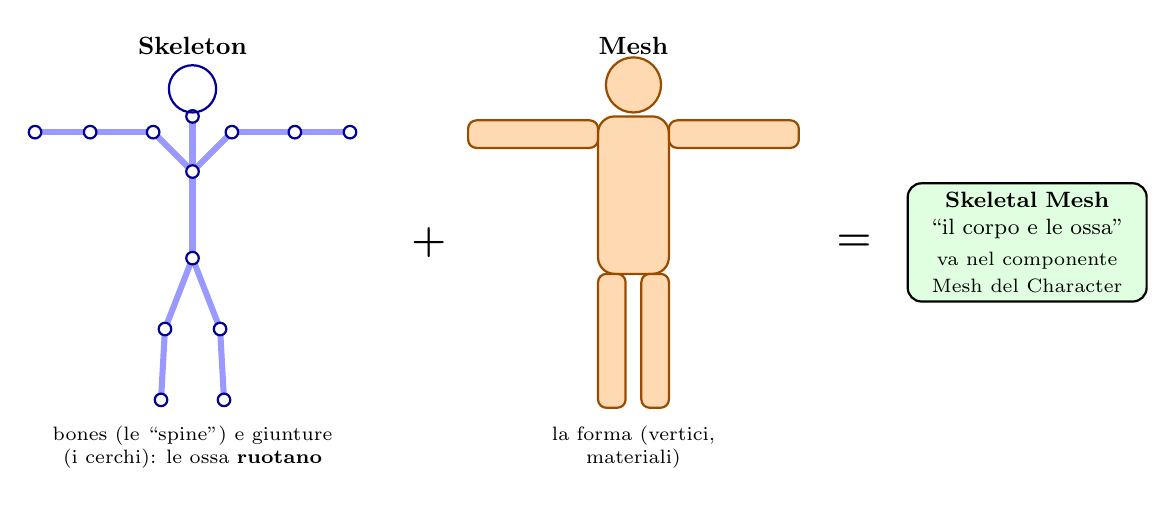
\begin{tikzpicture}[font=\footnotesize,
  ue8bone/.style={draw=blue!60!black, fill=blue!15, thick},
  ue8joint/.style={draw=blue!60!black, fill=white, thick, circle, inner sep=1.6pt}]
  % --- Skeleton (sinistra)
  \node[font=\small\bfseries] at (0,4.3) {Skeleton};
  \coordinate (pel) at (0,1.6); \coordinate (spi) at (0,2.7); \coordinate (nec) at (0,3.4);
  \coordinate (sl) at (-0.5,3.2); \coordinate (sr) at (0.5,3.2);
  \coordinate (el) at (-1.3,3.2); \coordinate (er) at (1.3,3.2);
  \coordinate (hl) at (-2.0,3.2); \coordinate (hr) at (2.0,3.2);
  \coordinate (kl) at (-0.35,0.7); \coordinate (kr) at (0.35,0.7);
  \coordinate (fl) at (-0.4,-0.2); \coordinate (fr) at (0.4,-0.2);
  \foreach \a/\b in {pel/spi, spi/nec, spi/sl, spi/sr, sl/el, sr/er, el/hl, er/hr,
                     pel/kl, pel/kr, kl/fl, kr/fr}
    \draw[ue8bone, line width=2.2pt, blue!40] (\a) -- (\b);
  \foreach \p in {pel, spi, nec, sl, sr, el, er, hl, hr, kl, kr, fl, fr}
    \node[ue8joint] at (\p) {};
  \draw[blue!60!black, thick] (0,3.75) circle (0.3);
  \node[font=\scriptsize, align=center] at (0,-0.8) {bones (le ``spine'') e
    giunture\\(i cerchi): le ossa \textbf{ruotano}};
  % --- piu'
  \node[font=\Large\bfseries] at (3.0,1.8) {+};
  % --- Mesh
  \begin{scope}[xshift=5.6cm]
    \node[font=\small\bfseries] at (0,4.3) {Mesh};
    \fill[orange!30, draw=orange!60!black, thick, rounded corners=6pt]
      (-0.45,1.4) rectangle (0.45,3.4);
    \fill[orange!30, draw=orange!60!black, thick] (0,3.8) circle (0.35);
    \fill[orange!30, draw=orange!60!black, thick, rounded corners=3pt]
      (-2.1,3.0) rectangle (-0.45,3.35);
    \fill[orange!30, draw=orange!60!black, thick, rounded corners=3pt]
      (0.45,3.0) rectangle (2.1,3.35);
    \fill[orange!30, draw=orange!60!black, thick, rounded corners=3pt]
      (-0.45,-0.3) rectangle (-0.1,1.4);
    \fill[orange!30, draw=orange!60!black, thick, rounded corners=3pt]
      (0.1,-0.3) rectangle (0.45,1.4);
    \node[font=\scriptsize, align=center] at (0,-0.8) {la forma (vertici,\\materiali)};
  \end{scope}
  % --- uguale
  \node[font=\Large\bfseries] at (8.4,1.8) {=};
  \node[draw, thick, rounded corners=5pt, fill=green!12, align=center, text width=2.8cm]
    at (10.6,1.8) {\textbf{Skeletal Mesh}\\``il corpo e le ossa''\\[2pt]
    \scriptsize va nel componente Mesh del Character};
\end{tikzpicture}
\caption{Skeletal Mesh e Skeleton secondo la lezione: due asset diversi. Lo Skeleton è
la gerarchia delle ossa, con le giunture; la Skeletal Mesh è la forma legata a quelle
ossa. Le animazioni sono rotazioni delle ossa, e sono legate allo Skeleton. Schema
ricostruito, non in scala.}
\label{ue8:fig:skeletal}
\end{figure}

\paragraph{Approfondimento: perché due asset.} Romero e Sewell (capitolo 17, ``Animation
Blueprints'') spiegano la separazione così: ``uno Skeleton è una gerarchia di ossa
interconnesse, usata per animare i vertici poligonali di una Skeletal Mesh''; e
``siccome l'animazione è fatta sullo Skeleton, può essere condivisa da molte Skeletal
Mesh che usano lo stesso Skeleton''. È il motivo per cui un gioco può avere decine di
personaggi diversi con un solo set di animazioni, e il motivo per cui, più avanti, le
animazioni del manichino di Unreal potranno essere \emph{ritargettate} sul cavaliere di
Mixamo, che ha uno scheletro simile ma non identico. Gli autori elencano anche i cinque
editor che si aprono dagli asset di animazione, con i bottoni in alto a destra già visti
dal docente: \emph{Skeleton Editor}, \emph{Skeletal Mesh Editor}, \emph{Animation
Editor}, \emph{Animation Blueprint Editor} e \emph{Physics Asset Editor}.

% ---------------------------------------------------------------------
\section{Le animazioni di Mixamo}
\label{ue8:sec:mixamoanim}

``Torniamo su Mixamo.'' L'importante è che nella viewport di Mixamo ci sia il proprio
personaggio, ``non un altro''; poi si passa alla categoria \textbf{Animations}. Servono
\textbf{tre animazioni} principali: \textbf{idle}, \textbf{walk} e \textbf{run}. ``La
idle, per chi non lo sapesse, sono le animazioni di stallo'': il personaggio ``sta fermo,
sta respirando'', il \emph{breathing}.

\paragraph{I controlli di Mixamo.} Sulla destra, per ogni animazione, ci sono alcuni
cursori; il docente li prova su animazioni diverse per farli vedere bene:
\begin{itemize}
  \item \textbf{Overdrive}: la velocità dell'animazione. ``Se aumento l'overdrive,
        questa animazione si velocizza sempre di più; se lo diminuisco, sarà
        lentissima'';
  \item \textbf{Character Arm-Space}: su alcuni modelli, la distanza delle braccia dal
        corpo, ``diventa sempre di più oppure diminuisce''. Attenzione al
        \emph{clipping}, le braccia che entrano nel corpo: ``infatti clippa
        malissimo''. Il docente suggerisce valori intorno a 50;
  \item \textbf{Trim}: ``tagliare l'animazione'', prenderne solo un pezzo. Ma ``viene
        fuori malissimo, perché non c'è il ritorno all'idle'': l'animazione tagliata non
        si chiude su sé stessa;
  \item \textbf{Mirror}: presente solo su alcune animazioni, ``semplicemente flippa
        l'animazione'', la \emph{specchia}. Il docente lo mostra con una Capoeira.
\end{itemize}

\paragraph{Root motion e in place.} Il punto più importante. Il docente apre un
\emph{Walking}: ``vedete che il character sta andando dritto, cioè sta percorrendo dello
spazio''. ``Questa tipologia di animazione viene chiamata \textbf{root motion}'': le
animazioni in root motion ``ereditano il movimento già nell'animazione''. L'esempio è
\emph{Dark Souls 3} (``qualcuno ha giocato Dark Souls 3? Perfetto''): alcune armi hanno
abilità speciali, le \emph{weapon art}, e in un video il docente cerca quella della
\emph{Holy Sword} (``questa non è in root motion, perché sta ferma''; ``eccola, questa
qua''): ``quando io la compio, mi sposto nello spazio già nell'animazione''. ``Non sono
io che gli do il movimento quando premo il tasto'': ``metto il piede in avanti, o faccio
l'affondo'', e il personaggio avanza perché lo fa l'animazione. Le animazioni in root
motion ``spesso sono usate per abilità'' di questo tipo.

``In questo caso, però, su Mixamo non dobbiamo avere un'animazione root motion'', perché
``erediteremmo un movimento che non ci interessa''. ``Noi, a livello del nostro gioco su
Unreal, vogliamo che l'animazione si compia, ma quella che si muove è la
\textbf{capsula}'': ``l'animazione segue la capsula''; ``c'è la mesh con l'animazione su
quella capsula, e di conseguenza si crea il movimento, o l'illusione del movimento''.
Quindi si spunta \textbf{In Place}: ``come potete vedere, adesso l'animazione è sul
posto''. ``Se non trovate una spunta In Place, consiglio di cambiare animazione: ce ne
sono tante'' (figura~\ref{ue8:fig:rootmotion}).

\begin{figure}[htbp]
\centering
\begin{tikzpicture}[font=\footnotesize,
  ue8cap/.style={draw=blue!60!black, thick, rounded corners=7pt, minimum width=0.7cm,
                 minimum height=1.6cm},
  ue8arr/.style={-{Stealth[length=2.4mm]}, very thick}]
  % root motion
  \node[font=\small\bfseries, anchor=west] at (-0.6,2.2) {Root motion};
  \node[ue8cap, fill=blue!8] at (0.3,0.9) {};
  \fill[orange!60] (0.3,1.5) circle (0.14);
  \draw[orange!60!black, very thick] (0.3,1.35) -- (0.3,0.75) -- (0.1,0.2);
  \draw[orange!60!black, very thick] (0.3,0.75) -- (0.5,0.2);
  \foreach \x/\o in {1.6/40, 2.9/60, 4.2/100} {
    \fill[orange!\o] (\x,1.5) circle (0.14);
    \draw[orange!\o!black, very thick] (\x,1.35) -- (\x,0.75) -- (\x-0.2,0.2);
    \draw[orange!\o!black, very thick] (\x,0.75) -- (\x+0.25,0.2);
  }
  \draw[ue8arr, orange!70!black] (0.6,-0.2) -- node[below, font=\scriptsize]
    {è l'animazione a spostare la mesh} (4.4,-0.2);
  \node[font=\scriptsize, align=left, text width=4.6cm, anchor=west] at (-0.6,-1.2)
    {la capsula resta indietro: mesh e collisione si separano. Utile per affondi e
    abilità (le weapon art di \emph{Dark Souls 3}), con Enable Root Motion};
  % in place
  \begin{scope}[xshift=7.4cm]
    \node[font=\small\bfseries, anchor=west] at (-0.6,2.2) {In place};
    \foreach \x/\o in {0.3/40, 1.6/60, 2.9/80, 4.2/100} {
      \node[ue8cap, fill=blue!8] at (\x,0.9) {};
      \fill[orange!\o] (\x,1.5) circle (0.14);
      \draw[orange!\o!black, very thick] (\x,1.35) -- (\x,0.75) -- (\x-0.2,0.2);
      \draw[orange!\o!black, very thick] (\x,0.75) -- (\x+0.25,0.2);
    }
    \draw[ue8arr, blue!60!black] (0.6,-0.2) -- node[below, font=\scriptsize]
      {è il Character Movement a spostare la capsula} (4.4,-0.2);
    \node[font=\scriptsize, align=left, text width=4.6cm, anchor=west] at (-0.6,-1.2)
      {l'animazione cammina sul posto, e la mesh segue la capsula: è quello che serve per
      idle, walk e run};
  \end{scope}
\end{tikzpicture}
\caption{Root motion e in place. In un'animazione root motion lo spostamento è dentro
l'animazione; in un'animazione in place il personaggio cammina sul posto, e a muoversi
nel mondo è la capsula del Character. Per la locomozione di base la lezione usa solo
animazioni in place. Schema ricostruito.}
\label{ue8:fig:rootmotion}
\end{figure}

\paragraph{Le impostazioni di download.} Al download Mixamo chiede alcune opzioni
(tabella~\ref{ue8:tab:mixamo}):
\begin{itemize}
  \item \textbf{Format}: \textbf{FBX Binary}, ``ci va bene così'';
  \item \textbf{Frames per Second}: \textbf{30}. ``Le animazioni devono essere allo
        stesso tipo di frame'': ``meglio sempre prenderle tutte quante allo stesso
        numero di frame'', ``perché se no avete dei problemi'', soprattutto ``nel
        \emph{blending}, cioè nel mixare'' due animazioni con frame rate diversi;
  \item \textbf{Skin}: \textbf{Without Skin}. ``La skin è se volete prendere
        l'animazione con il modello: non ci interessa, perché il modello ce l'abbiamo
        già'';
  \item \textbf{Keyframe Reduction}: \textbf{none}, ``non ci interessa'' ridurre i
        keyframe.
\end{itemize}
Il docente scrive in chat le tre animazioni da cercare, ``idle, walk e run/sprint'',
lasciando ``la libertà di scegliere quelle che volete'': ``importante che abbiate
un'animazione che respira, sta fermo, eccetera, una che cammina e una che fa lo
sprint''. Lui ha preso \emph{Idle}, \emph{Walking} e \emph{Slow Run}. ``Vi lascio 5, 10
minuti.''

\begin{table}[htbp]
\centering
\small
\begin{tabular}{@{}p{3.2cm}p{3.6cm}p{7.2cm}@{}}
\toprule
\textbf{Opzione} & \textbf{Valore} & \textbf{Perché} \\
\midrule
\multicolumn{3}{@{}l}{\emph{Personaggio}} \\
Format & FBX Binary & il formato che Unreal importa \\
Pose & T-Pose & la posa di riferimento del rig; togliere l'animazione applicata (la X) \\
\midrule
\multicolumn{3}{@{}l}{\emph{Animazioni (idle, walk, run)}} \\
Format & FBX Binary & come sopra \\
Skin & Without Skin & il modello c'è già: serve solo il movimento delle ossa \\
Frames per Second & 30 & tutte allo stesso frame rate, per non avere problemi nel
blending \\
Keyframe Reduction & none & nessuna riduzione dei keyframe \\
In Place & spuntato & niente root motion: a muoversi è la capsula \\
Overdrive, Arm-Space, Trim, Mirror & a piacere & velocità, distanza delle braccia
(attenzione al clipping), taglio, specchio \\
\bottomrule
\end{tabular}
\caption{Le impostazioni di download di Mixamo indicate a lezione.}
\label{ue8:tab:mixamo}
\end{table}

\paragraph{Approfondimento: Mixamo e Unreal.} Mixamo è un servizio gratuito di Adobe, a
cui si accede con un account Adobe; personaggi e animazioni si possono usare anche in
progetti commerciali. Il suo rig ha una gerarchia simile a quella del manichino di
Unreal (Manny e Quinn), ma i nomi delle ossa sono diversi (le ossa di Mixamo hanno il
prefisso \emph{mixamorig:}), e manca un osso \emph{root} alla base, sotto il bacino.
Per questo le animazioni di Mixamo in root motion non funzionano bene in Unreal senza
correzioni: lo spostamento è registrato sull'osso del bacino (\emph{Hips}) invece che su
un root. Con le animazioni \emph{In Place}, come quelle della lezione, il problema non si
pone. La mancanza dell'osso root e i nomi diversi sono anche il motivo per cui, per usare
sul cavaliere le animazioni del manichino (il salto, la caduta), servirà il
\textbf{retargeting} annunciato dal docente, con gli asset \emph{IK Rig} e \emph{IK
Retargeter} di Unreal Engine 5.

% ---------------------------------------------------------------------
\section{Importare le animazioni sullo scheletro}
\label{ue8:sec:importanim}

Dopo i minuti di scelta (``ci siete tutti, ragazzi? Sì, perfetto'') si importano le
animazioni. I file scaricati hanno il nome dell'animazione (``slow run, walking,
eccetera''); ``l'importante è che ci sia FBX sopra''. Al docente una delle due versioni
di Walking era rotta, e usa \emph{Walking 1}. ``Consiglio: fate meglio una cartella'':
\textbf{Animation}. ``Fatela una per una, vi consiglio.''

\paragraph{Lo scheletro obbligatorio.} La finestra di import è ``praticamente la stessa
schermata'', ``ma differenza sostanziale'': in basso, \textbf{Import} è grigio, non si
può premere. ``Per l'animazione in particolare gli serve uno scheletro a cui adattare
l'animazione.'' Nella sezione \textbf{Common} c'è il campo \textbf{Skeleton}: si apre la
tendina, in cui compaiono ``tutti gli scheletri'', compreso quello del manichino ``che
usiamo per Unreal'', e si sceglie \emph{il proprio}, quello creato dall'import del
personaggio. ``A questo punto, Import vi diventa blu.'' Nella stessa finestra il docente
indica anche la spunta sull'import della sola animazione (nella trascrizione: ``fate sì
che Import Only Animation sia ok''); la frase che segue è confusa.

\paragraph{Targettare.} ``Ecco a voi che si è creata un'animazione.'' ``Il file di per sé
è a parte, però lui ha \textbf{targettato}'' (``prendete questo termine'') ``la nostra
animazione su quello scheletro in particolare''. Un'animazione appartiene a uno
scheletro, e si può usare solo con le mesh di quello scheletro.

\paragraph{Approfondimento: le opzioni di import di un'animazione.} Nella finestra FBX
di Unreal Engine 5, quando il campo \emph{Skeleton} è impostato e la spunta
\emph{Import Mesh} è tolta, Unreal importa \emph{solo} le animazioni contenute nel file,
senza creare un'altra Skeletal Mesh e un altro scheletro; con \emph{Import Animations}
attivo, ogni animazione diventa un asset \textbf{Animation Sequence}. È il caso dei file
di Mixamo scaricati \emph{Without Skin}, che contengono solo le ossa animate. Se invece
si lascia vuoto il campo Skeleton su un file con la mesh, Unreal crea uno scheletro nuovo
a ogni import: è facile ritrovarsi con due scheletri quasi identici (``mi sa che ci sono
due ragazzi che hanno importato due'' scheletri, osserva il docente sulla sua tendina) e
con animazioni non compatibili fra loro.

% ---------------------------------------------------------------------
\section{L'editor dell'animazione}
\label{ue8:sec:animeditor}

Con un doppio clic sull'animazione si apre l'\textbf{Animation Editor}, ``che vi permette
di visualizzare tutte le particolarità della nostra animazione''.

\paragraph{I controlli.} In basso c'è il pannello di controllo: andare al primo o
all'ultimo frame (\emph{To Front}, \emph{To End}), al frame precedente o successivo
(``frame per frame per frame''). ``Le animazioni sono costituite da frame'': questa ne ha
\textbf{30}. Con \textbf{spazio}, o con il pulsante, \emph{Play} e \emph{Pause}.

\paragraph{Asset Details.} Sul lato dell'editor c'è il pannello \textbf{Asset Details}
(``se non vedete una finestra, la potete trovare su Window $\rightarrow$ Asset Details'',
``o Finestra $\rightarrow$ Dettagli dell'asset, suppongo, in italiano''). Ci sono molti
dati ``che nessuno andrebbe a vedere''; le cose principali:
\begin{itemize}
  \item \textbf{Loop}: ``se questa animazione la vogliamo che vada in loop'': ``quando
        finisce, ricomincia'';
  \item \textbf{Rate Scale}: a 1 è la velocità normale; ``se metto 1,5 l'animazione è
        più veloce''; a 2 ancora di più; ``40, diventa un casino''. ``È un po' come
        l'overdrive che abbiamo visto'' su Mixamo;
  \item \textbf{Root Motion}: la spunta \emph{Enable Root Motion} non è attiva, ``va
        bene così'', perché l'animazione è in place.
\end{itemize}
Lo stesso per le altre due animazioni: Idle, Slow Run (``vi chiederà sempre lo
scheletro''). ``Se aprite le vostre animazioni, sono giuste, sono davanti a voi?'' Alla
fine: ``dovreste avere tutte e tre le nostre belle animazioni''.

% ---------------------------------------------------------------------
\section{L'Animation Blueprint}
\label{ue8:sec:abp}

``La domanda sorge spontanea: come facciamo a metterle su un character?'' Con
l'\textbf{Animation Blueprint}.

\paragraph{La creazione.} Nella cartella del personaggio (il docente l'ha chiamata
\textbf{Characters}) si crea una cartella \textbf{Blueprint}. Poi tasto destro,
\textbf{Animation $\rightarrow$ Animation Blueprint}. La finestra chiede ``di quale
scheletro'': si sceglie il proprio (il docente, ``il mio paladino''), \textbf{Create}, e il
nome: \textbf{ABP\_Knight}, con il prefisso ABP per \emph{Animation Blueprint} (``io ho
chiamato Knight, però voi chiamatelo Ciccio Baciccio''). A uno studente che non ha
capito, il docente ripete: ``Animation, Animation Blueprint; vi chiederà lo scheletro;
selezionate lo scheletro vostro''. L'Animation Blueprint ``sarà la logica, quindi la
parte di programmazione'' delle animazioni ``del nostro bellissimo nuovo character''.

\paragraph{L'editor.} ``L'Animation Blueprint è abbastanza pieno di roba'', ``ci si può
confondere facilmente''. Le parti:
\begin{itemize}
  \item a sinistra, la \textbf{preview}, con il cavaliere in T-pose: ``e va benissimo,
        perché è la sua forma base'';
  \item l'\textbf{AnimGraph}, con il blocco \textbf{Output Pose}: ``tutti i calcoli che
        andremo a fare di animazioni'' si collegano a lui, ``e questo blocco ci dice:
        guarda, esce fuori questa roba'';
  \item l'\textbf{Event Graph}, ``come ce l'abbiamo in un classico Blueprint'', dove si
        possono ``creare e prendere variabili, modificare cose''.
\end{itemize}
``Esistono due ambienti particolari'': nel primo, l'AnimGraph, ``si ragiona per quanto
riguarda le animazioni''; nel secondo, l'Event Graph, ``a livello di programmazione''.

\paragraph{I due dati che servono.} Nell'Event Graph si devono ricavare due cose dal
personaggio:
\begin{enumerate}
  \item la \textbf{velocità}, ``perché vogliamo che la nostra animazione di camminata e
        di corsa, o di idle, sia relativa alla velocità che abbiamo al momento col
        character''. ``C'è una comunicazione tra i dati di gioco, quindi il movimento, e
        le animazioni'': ``dato un certo valore di velocità, cambia l'animazione'';
  \item se il personaggio \textbf{sta cadendo} o no, ``in modo da dire: guarda, sto
        saltando, sto iniziando a cadere; fammi un'animazione di salto, e fammi il loop
        del \emph{falling}''.
\end{enumerate}
Le animazioni di salto e caduta ``non le abbiamo importate'': ``le andremo a
ritargettare in seguito'', perché ``Unreal ci mette a disposizione la possibilità di
ritargettare delle animazioni'', ``ma non lo vedremo adesso''.

\paragraph{Event Blueprint Initialize Animation.} Il primo nodo è \textbf{Event Blueprint
Initialize Animation}: ``dice: quando l'animazione inizia''. ``Come abbiamo visto, gli
eventi come il Begin Play vengono fatti quando viene inizializzato tutto'': questo ``è il
Begin Play, ma per le animazioni''. (A questo punto Unreal si blocca di nuovo:
``è crashato Unreal; direi che oggi è proprio una gran roba''. ``Mi sa che mi tocca
svuotare un po' di memoria.'' Liberata la memoria, si riparte.)

\paragraph{Try Get Pawn Owner.} Dall'evento si chiama \textbf{Try Get Pawn Owner}.
``Questo blocco ci permette di comunicare con il nostro Pawn'', ``il nostro player''.
``Immaginatevi due ambienti separati'': nel Gameplay Framework ``il Pawn è quello che
controlla il character'', mentre l'animazione ``è subordinata al Pawn''. ``Quindi andiamo
a dire: ehi, provami a prendere l'owner, cioè il pawn owner.'' Poi ``andiamo a fare un
cast: abbiamo detto BP\_Knight\ldots{} Ah, giusto, ragazzi. Abbiamo scordato una cosa.
Dobbiamo creare effettivamente il nostro character.''

% ---------------------------------------------------------------------
\section{Il nuovo Character: BP\_Knight1}
\label{ue8:sec:character}

``Dobbiamo comunicare con il nostro character, per dire: guarda, mi servono questi dati
del movimento.'' Nella cartella Blueprint del personaggio: \textbf{Blueprint Class}, e
``attenzione'': come genitore si sceglie \textbf{Character}. Il nome:
\textbf{BP\_Knight1}.

\paragraph{I componenti del Character.} ``I character, a differenza degli actor, sono
costituiti di base da'':
\begin{itemize}
  \item un \textbf{Capsule Component}, la capsula;
  \item una \textbf{freccia} (\emph{Arrow}), ``per far capire qual è il forward vector
        della capsula'';
  \item la \textbf{Mesh}, una Skeletal Mesh;
  \item il \textbf{Character Movement}, ``il componente che definisce il movimento del
        character''. Nei suoi Details, in \emph{General Settings}, ci sono la
        \textbf{Gravity Scale}, la \textbf{Max Acceleration}, la \textbf{Braking
        Friction}. ``Come abbiamo detto, dobbiamo interfacciare le animazioni con i
        valori del movimento'', e quei valori stanno qui.
\end{itemize}

\paragraph{La Skeletal Mesh.} Nella Mesh si assegna la Skeletal Mesh del cavaliere (``devo
ricordarmi l'indirizzo''; ``no, non è questo, è questo qua''). Il personaggio ``è apparso
in modo abbastanza scorretto'', fuori posto rispetto alla capsula e girato male: ``basta
riposizionarlo''. ``Consiglio di fare lo \textbf{snapping}'': si abbassa la mesh in modo
che i piedi tocchino il fondo della capsula, e la si ruota ``in direzione della capsule'',
cioè con la faccia nella direzione della freccia (per i personaggi di Mixamo
serve di solito una rotazione di $-$90 gradi sulla Z; il valore esatto la trascrizione
non lo dice). ``Eccovi che abbiamo creato il nostro primo character.
Questa è la T-pose, meraviglioso.''

\paragraph{L'Anim Class.} ``Ma in questo caso non ha ancora animazioni.'' ``Come facciamo
a dire: guarda, devi usare proprio questa Animation Blueprint?'' Nella \textbf{Mesh}, alla
voce \textbf{Anim Class}, la tendina mostra tutti gli Animation Blueprint compatibili:
si sceglie \textbf{ABP\_Knight1} (il nome dell'asset del docente). ``Non è cambiato
niente, ma l'abbiamo messo in comunicazione'': quando l'Animation Blueprint avrà delle
animazioni, ``questo qua si aggiornerà''. La relazione è a due vie: il Character dice
quale Animation Blueprint usare (Anim Class), e l'Animation Blueprint chiede al suo
proprietario i dati (Try Get Pawn Owner).

% ---------------------------------------------------------------------
\section{Initialize: il cast e le referenze}
\label{ue8:sec:initialize}

Tornati nell'Animation Blueprint, il grafo dell'inizializzazione si completa
(figura~\ref{ue8:fig:abpgraph}, in alto):
\begin{enumerate}
  \item \textbf{Event Blueprint Initialize Animation};
  \item \textbf{Try Get Pawn Owner} $\rightarrow$ \textbf{Cast To BP\_Knight1}
        (``castate al vostro character, come l'avete chiamato'');
  \item dal pin As BP Knight1, \textbf{Promote to Variable}: una variabile referenza
        \textbf{BP\_Knight1}. ``Andiamo a creare una referenza del character, in modo
        tale che sia più semplice'': ``ogni volta che dovremmo prendere una cosa del
        character, dovremmo, se no, fare sempre Cast To BP\_Knight'', ed ``appesantisce
        castare sempre un qualcosa. Quindi lo facciamo all'inizio'';
  \item dalla referenza, \textbf{Get Character Movement}, ``per essere anche un po' più
        esaustivi'', e anche questo \textbf{Promote to Variable}: una variabile
        \textbf{MovementComponent}. ``Abbiamo creato già due variabili che ci faranno
        comodo in seguito.''
\end{enumerate}

\paragraph{Approfondimento: lo stesso grafo del modello Third Person.} Il grafo costruito
dal docente ricalca quasi nodo per nodo l'Animation Blueprint del manichino di Unreal
Engine 5 (\emph{ABP\_Manny}, nel modello Third Person): sull'Initialize, Try Get Pawn
Owner, Cast To Character, Set \emph{Character}, Get Character Movement, Set
\emph{MovementComponent}; sull'Update, controllo di validità, poi Set \emph{Velocity},
Set \emph{GroundSpeed} (Vector Length XY), Set \emph{ShouldMove} e Set \emph{IsFalling}.
La differenza è il cast: il modello fa Cast To \emph{Character}, la classe generica,
così che lo stesso Animation Blueprint funzioni con qualsiasi personaggio basato su
Character; la lezione fa Cast To BP\_Knight1, che dà accesso anche alle variabili
aggiunte nel cavaliere (utile, per esempio, per uno sprint), ma lega l'ABP a quella
classe.

% ---------------------------------------------------------------------
\section{Update: la velocità e la caduta}
\label{ue8:sec:update}

\paragraph{Event Blueprint Update Animation.} ``Questo evento avviene quasi come il Tick,
a ogni frame.'' ``Quando un'animazione si aggiorna, qualsiasi micro movimento è un
Update'': ``se abbiamo un idle, comunque è un'animazione; un walk, comunque è
un'animazione; e il run, comunque è un'animazione'', ``quindi sarà sempre attivo''. ``È
per questo che non facciamo il cast qui'': ``se no farebbe ogni volta, ogni frame,
sempre molto pesante''.

\paragraph{Il Validated Get.} ``Dobbiamo vedere se questo character è valido.'' ``Vi
ricordate gli Is Valid? Se in una variabile c'è qualcosa dentro o non c'è.'' C'è ``una
cosa molto interessante'': si trascina nel grafo un \textbf{Get} della variabile
BP\_Knight1, tasto destro, \textbf{Convert to Validated Get}. Il Get ``normale'' prende la
variabile e basta; il Validated Get ``prende la variabile, e mette anche la
particolarità: se lo prendo ed è valido faccio questo, se non è valido faccio
quest'altro''. Ha un ingresso di esecuzione e due uscite, \textbf{Is Valid} e \textbf{Is
Not Valid}: un Get e un Is Valid in un nodo solo. Sull'uscita Is Valid il docente mette
una \textbf{Sequence} (``un Is Valid, Sequence'') per eseguire in ordine le operazioni
che seguono.

\paragraph{GroundSpeed.} ``Fondamentalmente andiamo a prendere il Movement Component'',
la variabile creata nell'Initialize, e da lì \textbf{Get Velocity}: ``la velocità attuale,
a ogni frame, del character movement''. È un vettore; ``ci interessa solamente il
movimento'' sul piano, ``non ci interessa se salta o meno'', ``quello ci interesserà in
altro modo''. Quindi il nodo \textbf{Vector Length XY}: ``la lunghezza del vettore
solamente sugli assi X e Y'', ``se l'asse X è avanti e dietro e l'asse Y è destra e
sinistra''. Il risultato è un \textbf{float}, e diventa, con \textbf{Promote to
Variable}, \textbf{GroundSpeed}: ``una variabile che rappresenta la nostra velocità
attuale''.

\paragraph{IsFalling.} ``Molto importante per sapere quando saltiamo o quando stiamo
cadendo'': dal Movement Component, il nodo \textbf{Is Falling}. ``Ce ne sono due'': uno è
quello del \emph{Nav Movement}; quello giusto ``deve essere blu all'inizio e rosso alla
fine'', cioè con l'ingresso target blu (il Character Movement) e l'uscita rossa (una
booleana). Il valore va in una variabile, \textbf{IsFalling}, aggiornata a ogni frame,
``in modo tale da sapere che movimento fargli fare'' nel ``giro di animazioni''.

\paragraph{Velocity.} ``Per il futuro, per altre cose che ci serviranno'', anche il
vettore della velocità si promuove a variabile: \textbf{Velocity}, ``così almeno ci sono
delle cose che vogliamo interfacciare con la velocità''. ``Adesso abbiamo tirato fuori la
nostra velocità attuale e il fatto se sta cadendo o meno.'' A uno studente il Get
Velocity non compare: è quello che si ottiene dal Movement Component, con il target
giallo e l'uscita gialla (un vettore); cercandolo in fondo alla lista, ``trovato''.

\begin{figure}[htbp]
\centering
\begin{tikzpicture}[font=\footnotesize,
  ue8node/.style={draw, thick, rounded corners=4pt, align=center, fill=gray!8,
                  minimum height=0.8cm, text width=2.0cm},
  ue8ev/.style={ue8node, fill=red!12},
  ue8pure/.style={ue8node, fill=green!10, rounded corners=8pt},
  ue8var/.style={ue8node, fill=blue!10, rounded corners=8pt},
  ue8exec/.style={-{Stealth[length=2.5mm]}, very thick, black!80},
  ue8data/.style={-{Stealth[length=2mm]}, thick, blue!60!black}]
  % Initialize
  \node[font=\small\bfseries, anchor=west] at (-1.2,1.3) {Inizializzazione (una volta)};
  \node[ue8ev, text width=2.3cm] (ini) at (0,0) {\textbf{Event Blueprint Initialize
    Animation}};
  \node[ue8node, fill=blue!10, text width=1.9cm] (cst) at (3.2,0) {\textbf{Cast To}\\
    BP\_Knight1};
  \node[ue8pure] (tgp) at (3.2,-1.6) {\textbf{Try Get}\\\textbf{Pawn Owner}};
  \node[ue8node, text width=2.0cm] (s1) at (6.2,0) {\textbf{Set}\\BP\_Knight1};
  \node[ue8node, text width=2.8cm] (s2) at (9.6,0) {\textbf{Set}\\Movement\-Component};
  \node[ue8pure, text width=2.6cm] (gcm) at (9.6,-1.6) {BP\_Knight1 $\rightarrow$\\
    \textbf{Get Character Movement}};
  \draw[ue8exec] (ini) -- (cst);
  \draw[ue8data] (tgp) -- node[right, font=\scriptsize]{Object} (cst);
  \draw[ue8exec] (cst) -- (s1);
  \draw[ue8exec] (s1) -- (s2);
  \draw[ue8data] (gcm) -- (s2);
  % Update
  \node[font=\small\bfseries, anchor=west] at (-1.2,-3.1) {Aggiornamento (ogni frame)};
  \node[ue8ev, text width=2.3cm] (upd) at (0,-4.6) {\textbf{Event Blueprint Update
    Animation}};
  \node[ue8var, text width=2.0cm] (vg) at (3.3,-4.6) {\textbf{Validated Get}\\
    BP\_Knight1};
  \node[ue8node, text width=1.6cm] (seq) at (6.5,-4.6) {\textbf{Sequence}};
  \node[ue8node, text width=3.6cm, align=left] (sv) at (10.6,-3.4) {\textbf{Set
    Velocity} $\leftarrow$\\MovementComponent $\rightarrow$ Get Velocity};
  \node[ue8node, text width=3.6cm, align=left] (sg) at (10.6,-4.7) {\textbf{Set
    GroundSpeed} $\leftarrow$\\Vector Length XY (Velocity)};
  \node[ue8node, text width=3.6cm, align=left] (sf) at (10.6,-6.0) {\textbf{Set
    IsFalling} $\leftarrow$\\MovementComponent $\rightarrow$ Is Falling};
  \draw[ue8exec] (upd) -- (vg);
  \draw[ue8exec] (vg) -- node[above, font=\scriptsize]{Is Valid} (seq);
  \draw[ue8exec] (seq.east) -- ++(0.4,0) |- node[pos=0.75, above, font=\scriptsize]
    {Then 0} (sv.west);
  \draw[ue8exec] (seq.east) -- ++(0.4,0) |- node[pos=0.75, above, font=\scriptsize]
    {Then 1} (sg.west);
  \draw[ue8exec] (seq.east) -- ++(0.4,0) |- node[pos=0.75, above, font=\scriptsize]
    {Then 2} (sf.west);
\end{tikzpicture}
\caption{I due grafi dell'Event Graph di ABP\_Knight. In alto, una sola volta: si prende
il proprietario, lo si converte nel cavaliere e si salvano due referenze. In basso, a
ogni frame: se la referenza è valida, si aggiornano Velocity (vettore), GroundSpeed (la
sua lunghezza sul piano XY) e IsFalling (booleana). Accanto a ogni Set, il valore che riceve.
Schema ricostruito.}
\label{ue8:fig:abpgraph}
\end{figure}

\paragraph{Un registro di dati.} ``Questo graph funziona letteralmente come'' un
registro (la trascrizione dice ``registri di credito''): serve ``principalmente per
interfacciarsi con il nostro bellissimo character'', e ``ci serve per capire valori,
vedere cose'', ``parliamo di numeri per lo più''. Le animazioni vere si decidono altrove.

\paragraph{Approfondimento: perché l'AnimGraph non legge da solo.} Romero e Sewell
(capitolo 17) descrivono la stessa divisione dei compiti: ``usiamo l'EventGraph di un
Animation Blueprint per prendere i dati dal Pawn o dal Character che sta usando l'istanza
dell'Animation Blueprint, e per aggiornare le variabili dell'Animation Blueprint''; e
``l'AnimGraph può accedere solo alle variabili dell'Animation Blueprint''. Il loro esempio
è più semplice di quello della lezione: sull'Update un Is Valid sul Try Get Pawn Owner,
Get Velocity dal Pawn, \emph{VectorLength} (la lunghezza su tutti e tre gli assi) e Set
di una variabile \emph{Speed}. La scelta del docente, \textbf{Vector Length XY}, è più
precisa per la locomozione: con la lunghezza completa, un personaggio che cade dritto
verso il basso avrebbe una velocità alta e farebbe la corsa a mezz'aria. Gli autori
notano anche che \emph{Event Blueprint Update Animation} ha un parametro \emph{Delta Time
X}, il tempo trascorso dall'ultimo frame, utile per interpolare i valori.

% ---------------------------------------------------------------------
\section{L'AnimGraph, un'anteprima del Blend Space e il personaggio finito}
\label{ue8:sec:animgraph}

``Adesso, ragazzi, vi faccio una spiegazione teorica molto corta, perché capisco che siamo
agli ultimi dieci minuti, anzi sette.'' L'AnimGraph, ``differentemente, lavora per
esempio per \emph{state machine}''.

\paragraph{Un'animazione sull'Output Pose.} Il caso più semplice: nell'\textbf{Asset
Browser} dell'editor (``qua trovate tutte le animazioni che sono compatibili con questo
scheletro'') si prende un'animazione, per esempio \emph{Walking 1}, la si trascina
nell'AnimGraph e si collega ``l'omino'' del nodo all'omino dell'\textbf{Output Pose}. Non
è in loop, ma basta spuntare \textbf{Loop Animation} nei Details del nodo. Compile: nella
preview il cavaliere cammina. ``E possiamo vederlo anche nel nostro character'', perché
l'Anim Class ``ci ha permesso di dirgli: guarda, ehi, hai questo in eredità, hai questo
sotto di te, l'Animation Blueprint''. ``Ma, come potete capire, a noi serve molto di più
rispetto a mettere queste animazioni'' una alla volta.

\paragraph{Il Blend Space 1D.} ``Sicuramente la prossima volta andremo a vedere quelli
che sono chiamati \textbf{Blend Space}. Ve lo faccio vedere velocissimamente.'' Il
docente apre un \textbf{Blend Space 1D} (``una dimensione''), creato sullo scheletro del
cavaliere: un grafico con il personaggio che ``ci permette di mettere insieme varie
animazioni che \emph{blendano} tra di loro'', cioè ``che interpolano tra di loro''.
Nella preview, spostandosi sull'asse: idle, poi walking, poi sprint. ``In questo caso ci
sarà solamente un asse, che noi diremo che sarà la nostra \textbf{GroundSpeed}'', la
velocità ``che definisce il movimento'' (figura~\ref{ue8:fig:blendspace}). ``La prossima
volta vedremo di costruire questa tipologia di asset e collegare tutto quanto.''

\begin{figure}[htbp]
\centering
\begin{tikzpicture}[font=\footnotesize,
  ue8pt/.style={draw=black, fill=white, thick, diamond, inner sep=2.2pt}]
  \draw[-{Stealth[length=2.5mm]}, thick] (0,0) -- (11.2,0) node[right]{GroundSpeed};
  \foreach \x/\v in {0/0, 2.5/150, 5/300, 7.5/450, 10/600}
    \draw (\x,0.1) -- (\x,-0.1) node[below, font=\scriptsize]{\v};
  \node[ue8pt] (i) at (0,0) {}; \node[ue8pt] (w) at (2.5,0) {}; \node[ue8pt] (r) at
    (10,0) {};
  \node[above=6pt of i, font=\scriptsize\bfseries] {Idle};
  \node[above=6pt of w, font=\scriptsize\bfseries] {Walking};
  \node[above=6pt of r, font=\scriptsize\bfseries] {Run / Sprint};
  \fill[green!50!black] (6.25,0) circle (0.12);
  \draw[green!50!black, thick, ->] (6.25,0.9) -- (6.25,0.2);
  \node[green!40!black, font=\scriptsize, align=center] at (6.25,1.3) {valore attuale:
    50\% Walking + 50\% Run};
  \node[font=\scriptsize, align=center, text width=11cm] at (5.5,-1.0) {le animazioni
    sono campioni posti sull'asse; fra due campioni Unreal le mescola in proporzione
    alla distanza};
\end{tikzpicture}
\caption{Un Blend Space 1D come quello mostrato in anteprima: un solo asse, la
GroundSpeed calcolata nell'Event Graph, e tre animazioni poste su di esso. I valori
sull'asse sono un esempio, non quelli del docente. Schema ricostruito.}
\label{ue8:fig:blendspace}
\end{figure}

\paragraph{Il personaggio finito.} Per chiudere, il docente mostra dove arriveranno.
``Io posso cambiare il nostro character da qui'': nei \textbf{World Settings} del livello,
nella Game Mode, alla voce \textbf{Default Pawn Class}, sceglie BP\_Knight. In Play, il
cavaliere si muove con idle, camminata e corsa, e ``gli ho messo addirittura pure lo
sprint''. ``Il salto, questo è ritargettato'': è l'animazione classica di Unreal, portata
sullo scheletro di Mixamo. E la vecchia logica funziona con il nuovo personaggio:
``possiamo fare tutte le interazioni, e addirittura la nostra torretta ci segue''.
``Questo lo faremo la prossima volta'', ``perché ci vuole un pochino di continuità''.

\paragraph{Approfondimento: dalle animazioni singole alla State Machine.} Il capitolo 17
di Romero e Sewell mostra i passi successivi, quelli annunciati per la prossima lezione.
Un \textbf{Blend Space} è ``un tipo di asset che permette di mescolare animazioni in base
ai valori di uno o due parametri'': nel loro esempio del modello Third Person (UE4), il
Blend Space di locomozione pone \emph{Idle} a 0, \emph{Walk} a 93,75 e \emph{Run} a 375,
e con una velocità di circa 234 l'animazione risultante è metà camminata e metà corsa.
Trascinato nell'AnimGraph, il Blend Space diventa un nodo \emph{Blendspace Player} con un
ingresso per il parametro, a cui si collega la variabile della velocità; nell'\emph{Anim
Preview Editor} si può cambiare il valore e vedere il risultato senza andare in Play.
Poi la \textbf{State Machine}: un nodo dell'AnimGraph che organizza le animazioni in
\emph{stati} (per esempio \emph{Idle} e \emph{Moving}, e più avanti \emph{Jump} e
\emph{Fall}), collegati da \emph{transizioni} con regole booleane (per esempio
``GroundSpeed $>$ 3'' per passare da fermo a in movimento, o ``IsFalling'' per passare
al salto). È lì che la variabile IsFalling di oggi troverà il suo uso.

% ---------------------------------------------------------------------
\section{I materiali mancanti e la chiusura}
\label{ue8:sec:chiusura}

``Ci sono domande, ragazzi?'' Una studentessa: ``il mio personaggio non c'ha un
materiale, ha solo le texture''. ``Anche il mio non è importato'', aggiunge un altro.

\paragraph{Creare il materiale a mano.} La studentessa condivide lo schermo: il suo
personaggio di Mixamo è un'arciera (\emph{Erika Archer}, a giudicare dalla trascrizione).
``Se non hai un materiale, dovresti crearlo da zero'':
\begin{enumerate}
  \item tasto destro $\rightarrow$ \textbf{Material}, chiamato \textbf{M\_Archer};
  \item aperto il materiale in una finestra piccola, si trascinano dentro tutte le
        \textbf{texture} (``quelle con il label rosso''), che diventano nodi
        \textbf{Texture Sample};
  \item si legge bene il nome di ognuna: la \textbf{Diffuse} va nel \textbf{Base Color}
        (``acciaccala in Base Color''); la \textbf{Normal} va nel \textbf{Normal}.
\end{enumerate}
Leggendo i nomi, però, si scopre che le texture sono di due gruppi: una Diffuse dei
\emph{vestiti} e una della \emph{pelle} (e una delle ciglia, l'\emph{eyelash}). ``Ha due
materiali diversi, forse.'' ``Quindi mi sa che devi fare due materiali: uno per i
vestiti, e l'altro per la pelle'', per esempio \emph{M\_ArcherClothing}.

\paragraph{Gli slot dei materiali.} Per sapere dove va cosa, si apre la Skeletal Mesh:
nei Details, la sezione dei materiali mostra gli slot, con il \textbf{WorldGridMaterial}
(la griglia grigia di default) dove manca un materiale. Gli slot sono \emph{quattro}, non
due. Si mette il nuovo materiale nell'\textbf{Element 0} e si guarda ``dove te lo mette sul
corpo'': passando sopra uno slot, la parte corrispondente si illumina
(\emph{highlight}). Element 0 è il \emph{clothing}; il 2 e il 3 saranno la pelle, con un
altro materiale. ``Tanto, se non avete i materiali ma avete le texture, ragazzi, potete
farlo direttamente a mano.''

\paragraph{Le texture che non ci sono.} A un altro studente non sono state importate
nemmeno le texture. Il docente prova a riprodurre il problema: torna su Mixamo (``Mixamo
non mi risponde più, ottimo''), scarica lo stesso personaggio, \emph{The Boss}
(``use this character''; ``madonna mia''), in T-pose, e lo importa. Nella finestra di
import, nella sezione dei materiali, \textbf{Import Materials} e \textbf{Import
Textures} devono essere attivi (``fai sì che i materiali siano importati''); \emph{Import
Morph Targets} e simili ``non ci interessano''. ``A me importa tutto.'' ``Se c'hai
difficoltà, magari puoi semplicemente riprovare a fare l'import.'' Intanto Federico ha
risolto da solo, assegnando i materiali agli slot con l'highlight: ``allora vuol dire che
ti sei risolto la vita da solo. Perfetto.''

\paragraph{Approfondimento: Diffuse, Normal e gli altri canali.} Una \textbf{Diffuse} (o
\emph{Albedo}, o \emph{Base Color}) è il colore della superficie senza luci né ombre, e
va nel pin Base Color; una \textbf{Normal map}, riconoscibile dal colore azzurro-violetto,
simula i rilievi e va nel pin Normal (Unreal la riconosce all'import e imposta la
compressione \emph{Normalmap}). Se ci sono texture di \emph{Specular}, \emph{Roughness} o
\emph{Gloss}, vanno nei pin corrispondenti, ricordando che una Gloss è l'inverso di una
Roughness (serve un nodo \emph{1-x}, \emph{OneMinus}). Per le ciglia e i capelli, fatti
di piani con trasparenze, il materiale va impostato con \emph{Blend Mode} \emph{Masked}
e l'alfa della texture collegata all'\emph{Opacity Mask}: altrimenti le ciglia appaiono
come rettangoli pieni. Sono gli stessi nodi visti nella terza lezione, dedicata a
texture e materiali.

\paragraph{La chiusura.} ``Altri problemi? Se no, ci sentiamo la prossima volta.''
``Se dovete dichiarare qualcosa, non alla dogana, spero, ci sentiamo su Discord'':
``mandatemi quello che volete, se provate cose''. A Filippo: ``poi magari ti guardo un po'
quelle cosette che abbiamo visto prima''. ``Allora, ragazzi, buona cena, buona serata.
Ci vediamo giovedì. Ciao, ciao.''

\begin{table}[htbp]
\centering
\small
\begin{tabular}{@{}p{5.4cm}p{8.6cm}@{}}
\toprule
\textbf{Sintomo} & \textbf{Causa e rimedio} \\
\midrule
Una variabile ``non si muove'' & creata di nuovo e rimasta al default (0): controllare i
valori; variabili con nomi chiari \\
Errore sull'Audio Component ``non valido'' (Set Pitch Multiplier), solo arrivando in
fondo & caso rimasto aperto; ipotesi: lo Stop distrugge il suono (Auto Destroy) e la
variabile resta a puntare al vuoto. Is Valid, o Auto Destroy disattivato, o reset del Do
Once \\
L'ascensore va sempre più giù e non risale & attivazioni ripetute: booleana Activated
(Branch sul False all'inizio di Activation, false sul Begin Overlap) \\
Il progetto non si apre (si apre solo Unreal) & probabile chiavetta USB staccata male:
rimuoverla in sicurezza; usare un sistema di versione (Git) \\
Il personaggio si ferma un istante sul collezionabile & doppia collisione: mesh in
NoCollision, resta la Sphere Collision \\
On Component Begin Overlap non compare & è selezionata la mesh e non la Collision \\
Get Collectables non compare da Get Game Instance & manca il Cast To GI\_Platform: la
referenza è generica \\
Il cast non funziona & Get Game Instance non collegato all'Object del cast \\
``Non eredita da istanza di gioco''; la classe non compare nei Project Settings & la
Game Instance è stata creata con un altro genitore: ricrearla da GameInstance, sceglierla
in Game Instance Class, rifare variabile e cast \\
Il collezionabile conta ma l'esecuzione si ferma & il filo di esecuzione non passa per
il cast \\
Open Level non carica il livello & nome scritto male: è case sensitive. Copiarlo con F2,
Ctrl+C, Ctrl+V \\
Le palline raccolte riappaiono & normale: il livello viene ricaricato. Salvare lo stato
nella Game Instance (esercizio futuro) \\
Mettere a terra un componente nel Blueprint & nessuna scorciatoia (End vale solo nel
livello): regolare la Z a mano \\
Errore su Set Play Rate all'uscita dal Play & una vecchia referenza alla timeline con lo
stesso nome: eliminarla e usare quella giusta \\
Unreal si chiude durante l'import & memoria video esaurita: liberare memoria e spazio su
disco, reimportare \\
Il personaggio importato è ruotato & Offset Rotation non a zero: controllare Offset
Translation e Rotation all'import \\
Import grigio per un'animazione & manca lo Skeleton: sceglierlo in Common
$\rightarrow$ Skeleton \\
L'animazione sposta il personaggio da sola & è in root motion: riscaricarla da Mixamo
con In Place \\
Get Velocity non compare & cercarlo dal Movement Component (target e uscita gialli) \\
Il personaggio di Mixamo è grigio, senza materiale & creare i materiali a mano (Diffuse
in Base Color, Normal in Normal) e assegnarli agli slot; o reimportare con Import
Materials e Import Textures \\
\bottomrule
\end{tabular}
\caption{I problemi incontrati durante la lezione, con la causa e il rimedio.}
\label{ue8:tab:errori}
\end{table}

\begin{table}[htbp]
\centering
\small
\begin{tabular}{@{}p{4.6cm}p{9.4cm}@{}}
\toprule
\textbf{Nodo, asset o impostazione} & \textbf{Che cosa fa} \\
\midrule
Game Instance (Blueprint Class) & l'oggetto che vive per tutto il gioco; contiene dati
globali \\
Project Settings $\rightarrow$ Maps \& Modes $\rightarrow$ Game Instance Class & sceglie
la Game Instance del progetto \\
Get Game Instance & restituisce la Game Instance, come referenza generica \\
Cast To (classe) & converte una referenza nel tipo specifico; Cast Failed se non lo è \\
Increment Int (++) / Decrement Int ($--$) & aggiunge o toglie 1 a una variabile intera \\
Collision Presets: NoCollision & toglie ogni collisione a un componente \\
Sphere Collision, Sphere Radius & volume sferico e il suo raggio \\
Destroy Actor & distrugge l'actor \\
Evento Key (E) & scatta alla pressione di un tasto (Pressed, Released) \\
Text Render & un testo nel mondo 3D \\
Hidden in Game & nasconde un componente in gioco; tolto, la box si vede \\
Open Level (by Name) & carica un livello dal nome (case sensitive) \\
File $\rightarrow$ New Level (Basic) & un livello con cielo, luce e pavimento \\
Skeletal Mesh / Skeleton / Physics Asset & la mesh con le ossa; la gerarchia delle ossa;
i corpi fisici \\
Offset Translation / Rotation (import) & posizione e rotazione dell'asset rispetto al
pivot \\
Animation Sequence: Loop, Rate Scale, Enable Root Motion & ripetizione, velocità,
movimento dentro l'animazione \\
Animation Blueprint (ABP) & la logica delle animazioni di uno scheletro: Event Graph e
AnimGraph \\
Anim Class (Mesh del Character) & l'Animation Blueprint usato dalla mesh \\
Character (Capsule, Arrow, Mesh, Character Movement) & il Pawn che cammina, salta,
nuota, vola \\
Event Blueprint Initialize Animation & il ``Begin Play'' dell'Animation Blueprint \\
Try Get Pawn Owner & il Pawn che usa l'Animation Blueprint \\
Event Blueprint Update Animation & scatta a ogni aggiornamento dell'animazione, come il
Tick \\
Convert to Validated Get & un Get con le uscite Is Valid e Is Not Valid \\
Sequence & esegue più uscite in ordine \\
Get Velocity / Vector Length XY & la velocità; la sua lunghezza sul piano \\
Is Falling (Character Movement) & vero se il personaggio è in aria \\
Output Pose (AnimGraph) & la posa finale applicata alla mesh \\
Blend Space 1D & mescola animazioni lungo un asse (GroundSpeed) \\
World Settings $\rightarrow$ Default Pawn Class & il personaggio del giocatore in quel
livello \\
\bottomrule
\end{tabular}
\caption{I nodi, gli asset e le impostazioni dell'ottava lezione.}
\label{ue8:tab:nodi}
\end{table}

% ---------------------------------------------------------------------
\section*{Punti chiave del capitolo}
\addcontentsline{toc}{section}{Punti chiave del capitolo}

\begin{itemize}
  \item Il \textbf{Gameplay Framework} è la gerarchia delle entità che Unreal crea mentre
        il gioco gira: \textbf{Game Instance} (per tutta la durata del gioco), livello,
        \textbf{Game Mode} (le regole), \textbf{Game State} e \textbf{Player State} (lo
        stato, condiviso in rete), \textbf{Player Controller} (il ``cervello'' non
        fisico), \textbf{Pawn} e \textbf{Character} (il ``corpo''), e infine l'input.
  \item \textbf{Pubblica non vuol dire globale}: le variabili degli actor muoiono con il
        livello. Per conservare dati fra i livelli si usa la \textbf{Game Instance},
        creata come Blueprint Class da GameInstance e scelta in \textbf{Project Settings
        $\rightarrow$ Maps \& Modes $\rightarrow$ Game Instance Class}. Non va
        appesantita, perché resta in memoria per tutta la partita.
  \item \textbf{Get Game Instance} restituisce una referenza generica, ``la scocca'':
        per leggere le nostre variabili serve il \textbf{Cast To} della nostra classe,
        ``l'abito giusto'' per entrare alla festa. Cast Failed non è un errore, è una
        risposta.
  \item Un \textbf{collezionabile}: Sphere Collision, mesh in \textbf{NoCollision} (niente
        doppia collisione), controllo sul player, \textbf{Increment Int} sulla variabile
        della Game Instance, \textbf{Destroy Actor}.
  \item Un volume che cambia livello: \textbf{Open Level (by Name)} con il nome promosso
        a variabile pubblica. I nomi sono \textbf{case sensitive}: copiarli con F2 e
        Ctrl+C. I livelli nuovi da \textbf{File $\rightarrow$ New Level $\rightarrow$
        Basic}, salvati subito con Ctrl+S.
  \item Una booleana \textbf{Activated} con un Branch fa da cancello: l'ascensore
        ignora le attivazioni ripetute finché il player non lo fa risalire.
  \item Una \textbf{Skeletal Mesh} è ``il corpo e le ossa''; lo \textbf{Skeleton} è un
        asset separato, a cui sono legate le animazioni. Le ossa si \textbf{ruotano},
        non si spostano.
  \item Da \textbf{Mixamo}: personaggio in \textbf{T-pose}, \textbf{FBX Binary};
        animazioni idle, walk e run \textbf{In Place} (non root motion: a muoversi è la
        capsula), \textbf{Without Skin}, \textbf{30 fps} per tutte, nessuna riduzione dei
        keyframe. All'import si controllano gli \textbf{Offset}; le animazioni si
        importano scegliendo lo \textbf{Skeleton}.
  \item L'\textbf{Animation Blueprint} ha due grafi: l'\textbf{Event Graph} raccoglie i
        dati dal personaggio, l'\textbf{Anim\-Graph} decide la posa (\textbf{Output
        Pose}). Il Character lo usa tramite l'\textbf{Anim Class} della Mesh.
  \item Nell'\textbf{Initialize}: Try Get Pawn Owner, Cast To del personaggio, e le
        referenze salvate in variabili (il cast una volta sola). Nell'\textbf{Update},
        che gira a ogni frame: \textbf{Validated Get}, poi \textbf{GroundSpeed} (Vector
        Length XY della Get Velocity), \textbf{IsFalling} e \textbf{Velocity}.
  \item Prossimi passi: il \textbf{Blend Space 1D} sulla GroundSpeed, la State Machine,
        il \textbf{retargeting} del salto, e il personaggio impostato come
        \textbf{Default Pawn Class}.
\end{itemize}

%
%  Tutte le etichette di questo capitolo hanno il prefisso "ue8:"
%  (ue8:cap:..., ue8:sec:..., ue8:fig:..., ue8:tab:...), e tutti gli
%  stili TikZ hanno il prefisso "ue8" (ue8node, ue8exec, ue8data, ...)
%  per non collidere con chiavi native di TikZ né con quelli delle
%  lezioni precedenti. Il capitolo è autonomo: non contiene \ref verso
%  altri capitoli (i rimandi alle lezioni precedenti sono a parole).
%  Le figure sono ricostruzioni schematiche di quanto mostrato e detto a
%  lezione, non copie delle slide o delle schermate del docente. Dove la
%  trascrizione è troppo rovinata per ricostruire un dettaglio, il
%  capitolo lo dice invece di inventarlo.
% =====================================================================

\chapter[Game Instance, livelli e animazioni]{Game Instance, livelli e animazioni: il
Gameplay Framework e un nuovo personaggio}
\label{ue8:cap:gameinstance}

Questa è l'\textbf{ottava lezione} del corso breve di \textbf{introduzione a Unreal
Engine}. Nelle sette lezioni precedenti tutto è avvenuto dentro un solo livello e con un
solo personaggio, il manichino del modello Third Person: la torretta, i proiettili, la
piattaforma che sale, il pulsante che attiva le luci. Oggi la lezione allarga lo sguardo
in due direzioni. La prima è \textbf{uscire dal livello}: cambiare mappa senza perdere
quello che il giocatore ha fatto, cioè \textbf{salvare dei valori in modo globale}. La
seconda è \textbf{cambiare personaggio}: prendere un modello nuovo da \textbf{Mixamo},
importarlo con il suo scheletro e le sue animazioni, e cominciare a costruire la logica
che decide quale animazione mostrare, l'\textbf{Animation Blueprint}.

Il filo che tiene insieme le due parti è il \textbf{Gameplay Framework} di Unreal: la
``gerarchia'' delle entità che l'engine crea e tiene in vita mentre il gioco gira. La
\textbf{Game Instance}, la prima a nascere e l'ultima a morire, è il posto giusto per i
dati che devono sopravvivere al cambio di livello; il \textbf{Pawn} e il
\textbf{Character}, con il loro \textbf{Character Movement}, sono la fonte dei dati
(velocità, caduta) che l'Animation Blueprint legge per animare lo scheletro. ``Andremo
sia a vedere quelle che sono le animazioni e come si gestiscono, ma sia a vedere un po'
quello che è chiamato il \emph{gameplay framework} di Unreal.''

La lezione è \textbf{online}, su Zoom, come le precedenti, ma con una particolarità: la
webcam del docente si rifiuta di funzionare per tutta la serata (``oggi mi vedrete con
uno schermo nero, o almeno il mio schermo è più importante della mia faccia''), e in
due occasioni l'editor si chiude da solo per mancanza di memoria video. Si apre con un
problema di uno studente rimandato alla pausa, prosegue con una parte teorica in slide
sul Gameplay Framework e con la costruzione dei collezionabili, della Game Instance e
dei volumi che cambiano livello; la pausa arriva verso le 17:26, con ripresa alle ``55,
18, solito orario''; la seconda parte è dedicata all'import del personaggio e delle
animazioni e all'Animation Blueprint. Il docente stesso avverte che non si arriverà in
fondo: ``probabilmente questa lezione la riporteremo nella prossima'', in cui si vedranno
i Blend Space e il resto delle animazioni. Si chiude con un ``ci vediamo giovedì''.

Tre avvertenze di lettura, le stesse delle lezioni precedenti. La prima: la
trascrizione è automatica e storpia moltissimi nomi. Unreal è ``Arena Engine'',
``Arreal'', ``a Real'', ``a RIAL'', ``Arial'' e ``Irium'' (quest'ultimo, forse, è il
programma della webcam); la \textbf{Game Instance} è ``View Instance'', ``getViewInstance''
e ``key instance''; \textbf{GI\_Platform} è ``GI Gaming Instance'', ``gi i platform'',
``asg.platform'', ``giiPatform'' e ``Di Alto''; il \textbf{Pawn} è ``Pwn'', ``la Bone'' e
``player born''; \textbf{Get Player Pawn} è ``getLayerOne'' e ``PlayerOh''; il
\textbf{Cast To} è ``castagna''; l'\textbf{On Component Begin Overlap} è ``component
baking per l'acqua'', ``onBegin onComponent onBegin overlap'' e ``On Collision Beginner
per l'app''; il \textbf{Destroy Actor} è ``destroy hardware''; il \textbf{Text Render} è
``text rendere''; la \textbf{Skeletal Mesh} è ``scheletal mesh'' e ``scheda del Mesh''; il
\textbf{Control Rig} è ``control righe''; l'\textbf{Idle} è ``Idol''; il \textbf{root
motion} è ``root in''; la \textbf{T-pose} è ``Tico'', ``tifoso'' e ``Bix ti pose'';
\textbf{FBX Binary} è ``Fibix binary''; il \textbf{Knight} è ``Night''; il \textbf{Try Get
Pawn Owner} è ``try get one''; l'\textbf{Event Blueprint Update Animation} è ``event
blueprint a data animation''; \textbf{IsFalling} è ``isPalling''; il \textbf{Diffuse} è
``Diffuse'', ma l'\textbf{eyelash} è ``ailash''; \textbf{Mixamo} è a volte
``Mixamon''. Dove la ricostruzione è sicura il capitolo usa la forma corretta; dove non
lo è riporta la forma della trascrizione e lo dice. La seconda: all'inizio della
registrazione, durante la pausa e durante i minuti lasciati per scegliere le animazioni
il riconoscimento vocale produce lunghi blocchi di testo senza senso e ripetuto
(``grazie a tutti per l'attenzione che ci ha spiegato'', ``qual è la risposta che ci può
essere?'', ``la situazione è questa, la migliore dal 2005'', ``i genitori a bordo'', la
``dottrina sul mercato del lavoro'', un Vittorio Prodi chiamato in causa senza
motivo, una lunghissima fila di ``non, non, non''): sono artefatti, non parole di nessuno,
e il capitolo li ignora. La terza: gran parte della lezione è una dimostrazione dal vivo
nell'editor, costruita a voce (``tirate fuori'', ``castate'', ``promote to variable''),
e in un paio di punti il docente improvvisa o si accorge di aver saltato un passaggio
(``ah, giusto, ragazzi, abbiamo scordato una cosa''). Il capitolo ricostruisce i grafi da
ciò che il docente dice mentre li costruisce, e li completa, dove serve, con i nomi
esatti dei nodi e dei pin di Unreal Engine 5; dove la trascrizione lascia un buco, lo
dichiara.

\paragraph{Come leggere questo capitolo.} Il capitolo segue l'ordine della lezione. Le
figure ricostruiscono la gerarchia del Gameplay Framework, la vita della Game Instance
attraverso i cambi di livello, il cast come ``abito giusto'', i grafi del collezionabile,
del tasto E e dei due volumi, la differenza fra Skeletal Mesh e Skeleton, quella fra
animazione in root motion e in place, i due grafi dell'Animation Blueprint e il Blend
Space 1D. Le tabelle riassumono le entità del framework, le impostazioni di download di
Mixamo, gli asset creati dall'import, gli errori incontrati dagli studenti e i nodi della
giornata. Qua e là, dei paragrafi di \textbf{approfondimento} collegano la lezione ai
libri di Marcos Romero e Brenden Sewell (\emph{Blueprints Visual Scripting for Unreal
Engine 5} e la seconda edizione dello stesso testo, scritta per Unreal Engine 4), i
testi di riferimento per questa parte del libro, e a qualche nozione tecnica generale su
Unreal Engine 5; sono segnalati come tali e non fanno parte della lezione.

Il percorso del capitolo:
\begin{enumerate}
  \item l'\textbf{inizio della lezione}: un errore sul suono della piattaforma, Mixamo e
        le Game Jam (sezione~\ref{ue8:sec:inizio});
  \item il \textbf{programma}, le \textbf{variabili globali} e la dimostrazione dei
        collezionabili che passano da un livello all'altro (sezioni
        \ref{ue8:sec:programma} e~\ref{ue8:sec:demo});
  \item il \textbf{Gameplay Framework} di Unreal, dalla Game Instance all'input
        (sezione~\ref{ue8:sec:framework});
  \item il \textbf{fix dell'ascensore} con la booleana Activated
        (sezione~\ref{ue8:sec:ascensore});
  \item la \textbf{Game Instance}: creazione, variabile, Project Settings
        (sezione~\ref{ue8:sec:gi});
  \item il \textbf{collezionabile}, il \textbf{cast} e il tasto E (sezioni
        da~\ref{ue8:sec:collectible} a~\ref{ue8:sec:tastoe});
  \item i due \textbf{volumi}: lo shop che azzera e il volume che \textbf{carica un
        livello} (sezioni da~\ref{ue8:sec:shop} a~\ref{ue8:sec:prova});
  \item \textbf{Mixamo}, la pausa e i problemi degli studenti (sezioni
        \ref{ue8:sec:mixamochar} e~\ref{ue8:sec:pausa});
  \item l'\textbf{import} del personaggio, lo \textbf{scheletro} e le
        \textbf{animazioni} di Mixamo (sezioni da~\ref{ue8:sec:import}
        a~\ref{ue8:sec:animeditor});
  \item l'\textbf{Animation Blueprint}, il nuovo \textbf{Character} e l'AnimGraph
        (sezioni da~\ref{ue8:sec:abp} a~\ref{ue8:sec:animgraph});
  \item i \textbf{materiali} mancanti e la chiusura (sezione~\ref{ue8:sec:chiusura}).
\end{enumerate}

% ---------------------------------------------------------------------
\section{Prima della lezione: l'Audio Component, Mixamo e le Game Jam}
\label{ue8:sec:inizio}

La registrazione comincia con i saluti (``buonasera, buonasera, buonasera'') e con le
scuse del docente: ``scusate, ragazzi, se non mi faccio vedere, ma a quanto pare ho dei
problemi con la webcam''. Il sospetto è un conflitto con OBS, il programma di
registrazione (``forse OBS potrebbe fare contrasto''); i tentativi si ripetono per tutta
la prima parte, senza successo. ``Non vi preoccupate: vi guardo, mi ascoltate, ma non mi
vedete.''

\paragraph{Le variabili chiare.} ``Come state, ragazzi? Avete un po' sperimentato?''
Uno studente ha recuperato dalla registrazione la lezione del giovedì precedente, e
racconta il suo unico problema: ``non funzionava perché nella variabile non avevo messo
il tempo, e quindi non si muoveva niente''. Il docente ne fa una regola: ``il fatto di
avere delle variabili chiare e concise ti finisce proprio il lavoro'', perché altrimenti
``stai sempre là a riguardarle'' chiedendoti ``ma perché non si muove?'', finché non ti
ricordi ``che l'hai creata di nuovo, però sta a zero''. Una variabile appena creata ha
il suo valore di default (zero, per i numeri), e un tempo, una durata o una velocità
lasciati a zero fermano tutto senza dare errori.

\paragraph{Mixamo e le Game Jam.} Uno studente chiede se il sito condiviso su Discord sia
gratuito: ``sì, sì, assolutamente, non ci avete niente da spendere''. È
\textbf{Mixamo}, ``un'ottima risorsa'' che oggi verrà usata ``in modo attivo'': essendo
uno strumento di Adobe ``abbastanza preciso nel replicare le animazioni'', e avendo
modelli ``abbastanza compatibili'' con quelli di Unreal, permette di avere personaggi e
animazioni senza animarli a mano. ``Ci sono animazioni migliori, perché esistono i pack
che si pagano fior di quattrini'', ma per cominciare Mixamo è ``il ben di Dio''. Il
docente lo usa soprattutto per le \textbf{Game Jam}: ``uno ha mai fatto una Game Jam?''
Gli studenti rispondono da soli: ``sono gli eventi dove si programma un videogioco in
pochi giorni''. ``Fondamentalmente si programma il gioco in pochi giorni, che va dai tre
giorni a una settimana'', ``poi ognuno fa un po' come gli pare''; e in quei pochi giorni,
avere animazioni pronte è ciò che fa la differenza.

\paragraph{Il primo problema: l'Audio Component che non è valido.} Filippo condivide lo
schermo. La piattaforma della lezione precedente (``quando ho fatto il bottone, l'altra
volta'') funziona, il suono si sente, ``ma poi mi dà errore'', sul \textbf{Set Pitch
Multiplier}. Il docente insegna prima un'abitudine: nel log degli errori, quando un nome
è sottolineato, ``puoi direttamente cliccare: dice proprio l'errore e ti ci porta''. Il
messaggio, in italiano, è un tentativo di accesso a un componente ``tramite la proprietà
SoundPlatform'' che ``non è valida'': ``vuol dire che l'Audio Component non è stato
spawnato o non esiste''. L'errore compare solo salendo sulla piattaforma, e solo una
volta per partita: ``lo fa solo una volta, fortunatamente'', perché ``quelle successive te
lo fa''. È, a prima vista, lo stesso caso della settima lezione (il pitch impostato prima
che il suono esista), già incontrato con un'altra studentessa.

Il docente prova un rimedio rapido: togliere i due \emph{Get} di SoundPlatform (``questi
due cilindroni'') e collegare i due Set Pitch Multiplier direttamente all'uscita del
\emph{Set} della variabile, ``così dovremmo averci la sicurezza''. Non basta: rileggendo
l'errore, il problema ``non è SoundPlatform, è l'Audio Component'' a non essere valido.
``Visto che è una cosa che ci vuole un attimino di fuori programma'', il caso viene
rimandato alla pausa (sezione~\ref{ue8:sec:pausa}): ``può essere un errore di logica di
base, poi magari sono micro cose''.

\paragraph{Approfondimento: quando l'errore compare una volta sola.} Un errore di tipo
``Accessed None'' (``accesso nullo'', ``non è valida'') che compare \emph{solo la prima
volta} è quasi sempre un problema di \textbf{ordine}: un nodo legge una variabile
referenza prima che qualcuno l'abbia riempita. Dalla seconda volta in poi la variabile
contiene il suono spawnato la volta precedente, e tutto sembra funzionare. Un errore che
compare \emph{solo arrivando in fondo} (come dirà lo studente in pausa) indica invece che
il componente esisteva ma è stato distrutto: un Sound spawnato con \textbf{Spawn Sound at
Location} ha di default l'opzione \emph{Auto Destroy} attiva, cioè l'Audio Component si
distrugge da solo quando il suono finisce o viene fermato con \textbf{Stop}, e la
variabile rimane a puntare a un oggetto non più valido. In entrambi i casi la protezione
è la stessa: un \textbf{Is Valid} prima di usare la referenza, oppure ricreare il suono
quando serve.

% ---------------------------------------------------------------------
\section{Il programma della giornata e le variabili globali}
\label{ue8:sec:programma}

``Oggi andremo a vedere un po' di particolarità.'' Il programma ha due parti:
\begin{itemize}
  \item le \textbf{animazioni}, ``e come si gestiscono'';
  \item il \textbf{Gameplay Framework} di Unreal: il fatto che l'engine, ``nella sua
        esecuzione'', ha ``una gerarchia di quello che tiene, di quello che ha'', cioè
        di entità che ``sono sempre presenti in alcuni momenti''. Fra queste c'è la
        \textbf{Game Instance}, che oggi permetterà ``di salvare dei valori in modo
        globale, chiamiamolo così''.
\end{itemize}

\paragraph{Variabile globale e variabile locale.} ``Non so se qualcuno di voi, a livello
di programmazione, sa cosa si intende con una variabile globale'' (``Federico già lo vedo
bello arzillo''). Una \textbf{variabile globale} è ``visibile in tutte le parti del
codice'': ``indipendentemente dall'ambiente in cui ci troviamo'', nel character, in un
altro oggetto, nel livello, ``è possibile visualizzarla, prenderla, modificarla''.
L'esempio opposto è a portata di mano: la variabile \textbf{ActivableItems} del pulsante
della settima lezione. ``Questa è pubblica'', con l'occhietto aperto, ``la possiamo
vedere da viewport''; ma è pubblica solo nel senso che la si modifica nei Details
dell'istanza. Esiste \emph{dentro} quel pulsante, dentro quel livello: ``se noi dovessimo
cambiare mappa, questa variabile non la potremmo più vedere'', e ``se volessimo stampare
dei valori, questo qua non esisterebbe più''. Pubblica non vuol dire globale.

\paragraph{Approfondimento: pubblica, privata, globale.} Nei Blueprint le tre parole
indicano cose diverse. Una variabile \textbf{Instance Editable} (l'occhietto) è
modificabile nei Details di ogni istanza nel livello; una variabile \textbf{Private} non
è accessibile dagli altri Blueprint, nemmeno dai child; ma in tutti i casi la variabile
\emph{vive dentro un oggetto}, e muore con lui. Quando si apre un nuovo livello, Unreal
distrugge tutti gli actor del livello precedente, compreso il personaggio del giocatore,
e ne crea di nuovi: i valori delle loro variabili tornano ai default. Unreal non ha
variabili globali nel senso dei linguaggi testuali; il modo di ottenerle è appoggiarle a
un oggetto che \emph{non} viene distrutto al cambio di livello, ed è esattamente ciò che
la lezione fa con la Game Instance (sezione~\ref{ue8:sec:gi}).

% ---------------------------------------------------------------------
\section{La dimostrazione: collezionabili e porte fra i livelli}
\label{ue8:sec:demo}

Come sempre, prima di costruire il docente mostra il risultato finito. ``Adesso vedrete
anche questo nuovo character che andremo a creare da zero, grazie all'aiuto di Mixamo'',
con ``delle animazioni nuove''; e avverte che ``cambiare character, visto che tutto
quanto va a reagire con il character'' (la piattaforma, il pulsante, i controlli sul
player), richiederà ``un piccolo fix da fare''. Per la dimostrazione, quindi, rimette il
vecchio \textbf{ThirdPersonCharacter}.

\paragraph{I collezionabili.} Nel livello ci sono delle palline: ``questi sono dei
\emph{collectable}, sono delle palline che ho creato''. Il personaggio ci passa sopra,
``1, 2, 3'', e le palline spariscono; premendo il tasto \textbf{E}, sullo schermo
compare il numero di collezionabili presi: 3.

\paragraph{La porta e il nuovo livello.} ``Oggi creeremo anche questa, che è la
porticina, che ci porterà a un nuovo livello.'' Il personaggio la attraversa e si trova
in un livello quasi vuoto. Premendo E, il conteggio è ancora 3: ``interagendo con la Game
Instance, che è sempre presente indipendentemente se io cambio livello o meno, mi posso
trasportare dei valori''. Nel secondo livello ci sono altre palline: ``se prendo questa,
ne avrò 4'', poi 5 e 6; e ``se torno al mio hub, ne avrò 6''.

\paragraph{Crash Bandicoot.} ``Non so se qualcuno di voi ha giocato a Crash Bandicoot.''
I classici della serie tengono il conto dei \textbf{cristalli}, dei \textbf{frutti Wumpa}
(``frutti Pumpa'', nella trascrizione) e delle \textbf{gemme}: ``quelli sono valori che
sono sempre salvati quando tu li prendi'', che restano tali qualunque livello si
attraversi, ``quasi totalmente globali''. Senza la Game Instance, invece, ``si
perderebbe il valore'', e il conteggio ``tornerebbe sempre a zero'': ``dovresti fare
sempre 1, 2, 3, 1, 2, 3''.

\paragraph{Che cosa ancora non fa.} Tornando nel primo livello, le palline già raccolte
sono di nuovo lì: ``questo bellissimo collectible è rispawnato''. È il comportamento
normale (il livello viene ricaricato da capo), ed è anche il prossimo esercizio
annunciato: ``andremo a fare anche un esercizio del genere, in cui andremo a dire: ehi,
guarda che questo l'ho già raccolto, levalo, non me lo far riprendere''. Cioè
``salvarci globalmente lo stato delle cose''. Nella lezione di oggi l'esercizio non viene
svolto.

% ---------------------------------------------------------------------
\section{Il Gameplay Framework di Unreal}
\label{ue8:sec:framework}

\paragraph{Che cos'è un framework.} ``Qualcuno di voi sa che cosa si intende con
\emph{framework}? Ha mai usato un framework per qualsiasi cosa, per programmazione, o
semplicemente: a volte esistono i framework per la scrittura.'' Un framework è ``uno
sviluppo base di processi'', una ``scheda da seguire''. L'esempio del docente è la
narrativa: in una storia ``c'è l'inizio, c'è lo sviluppo, c'è magari il
\emph{cliffhanger}''; un horror può essere psicologico o splatter, un film d'azione
``demenziale'' o epico, e ognuno di questi generi, ``a scelta dell'autore'', può seguire
uno schema che ``lo aiuta a sviluppare un processo di creazione''. In Unreal ``esiste
praticamente questo tipo di processo'', fatto però di ``tante piccole interfacce'', o
meglio di \textbf{entità}, che ``hanno una gerarchia tra di loro''. ``Questo, ragazzi, è
il gameplay framework di Unreal.'' Il docente lo spiega su una slide con uno schema
dall'alto verso il basso, in ordine di nascita e di ``priorità''
(figura~\ref{ue8:fig:framework}).

\paragraph{La Game Instance.} ``Quando il progetto viene lanciato, cioè l'engine'', ``la
prima cosa che viene creata, o comunque che ha priorità, è la \textbf{Game Instance}.''
È un'entità ``che va a esistere sempre, in ogni caso, quando il gioco è aperto''. Subito
dopo, nello schema, viene il caricamento del \textbf{livello}.

\paragraph{La Game Mode e Gwent.} Con il livello nasce la \textbf{Game Mode}, ``un'altra
interfaccia, che in questo caso definisce gli stati di gioco, gli stati del giocatore,
oppure le \textbf{regole del gioco}''. ``Questa Game Mode esiste assieme alla mappa'',
``e di per sé nel mondo di gioco''. L'esempio è \emph{The Witcher 3} e il suo gioco di
carte, il \textbf{Gwent}: ``state giocando al gioco normale'', parlate con un NPC che vi
propone ``un round di carte'', ``e parte il gioco delle carte''. ``In quel caso la Game
Mode cambia'': ``le regole del gioco, i punteggi, le condizioni di vittoria o sconfitta
sono gestite dalla Game Mode''.

\paragraph{Game State, Player State, client e server.} Scendendo, lo schema mostra il
\textbf{Game State}, ``lo stato del gioco, quindi tutti i dati che sono presenti'', e il
\textbf{Player State}, ``lo stato del giocatore''. Servono soprattutto quando c'è un
``interscambio di dati'', come in una cooperativa o in un multigiocatore ``con un server
di mezzo''. Una seconda slide lo mostra: ``esiste il \textbf{client}'' (``avete presente
quando aprite quello che si chiama client'') e il \textbf{server}. ``Il client comunica
con un server, e va a mandare i dati ad altri giocatori con cui giocate online'': è così
che, in uno sparatutto, ``si capisce che tipo sei morto'' e che ``quel numero delle death
o delle kill aumenta'', ``perché c'è uno scambio di stati tra i nostri player''.

\paragraph{Il Pawn.} ``Abbiamo parlato di Pawn in precedenza'': il canale di collisione
\emph{Pawn}, il nodo \emph{Get Player Pawn} usato in ogni overlap. Il docente lo descrive
così: ``il Pawn non è già il character stesso, ma è l'entità'' che può essere
controllata, dal giocatore ``o addirittura dall'AI'', cioè ``o da input del giocatore,
oppure da un processo di \emph{behavior}, un comportamento già stabilito, come può essere
un nemico''. Al Pawn ``vengono date'' le componenti, la mesh, la navigazione, le
animazioni, il \emph{view target} (la camera) e, ``se ci fossero'', i \textbf{physical
material}, ``materiali che hanno delle proprietà fisiche'', da vedere più avanti.

\paragraph{Il Character e il Character Movement.} ``Il character stesso è subito dopo.''
Il Character ha ``le sue particolarità di movimento'', raccolte nel \textbf{Character
Movement Component}, con dati ``che possono essere modificati'':
\begin{itemize}
  \item le \textbf{movement mode}: ``come mi sto muovendo'', cioè se sta camminando, se
        sta volando (\emph{flying}), se sta nuotando, oppure un \emph{custom movement},
        ``un movimento particolare'', come una scivolata;
  \item le \textbf{movement capabilities}: ``quanto mi posso muovere, quanto veloce
        sono'', la \emph{braking friction}, ``cioè quanto ci metto a frenare'';
  \item le \textbf{interazioni fisiche};
  \item la \textbf{replicazione}, cioè il movimento condiviso in rete.
\end{itemize}

\paragraph{Skeletal Mesh e Skeleton.} Il Character ha anche la sua \textbf{mesh}, ``la
sua particolarità di avere la sua forma''. ``La Skeletal Mesh e lo scheletro sono due
cose completamente diverse, ragazzi.'' Lo \textbf{scheletro} è fatto di ossa, le
\textbf{bones}, ed è il prodotto del \textbf{rigging}, ``il compito di un povero ragazzo
o ragazza che si mette là a creare le ossa'', ``un lavoro a sé stante''; poi c'è
l'\textbf{animatore}, ``che ruota queste ossa per compiere un'animazione''. La
\textbf{Skeletal Mesh} ``è fondamentalmente una mesh con uno scheletro'': ``la forma più
le ossa'', ``il corpo e le ossa''. Lo scheletro è un asset separato, ``gestito in
un'altra modalità'', in cui si vedono ``tutte quante le ossa del nostro bellissimo
character'' (figura~\ref{ue8:fig:skeletal}). Le ossa si controllano con
l'\textbf{Animation Graph}, ``spesso chiamato Animation Blueprint'', che oggi verrà
creato, e con il \textbf{Control Rig}, ``una cosa che è stata messa da Unreal'' per
animare direttamente nell'editor, che però oggi ``non ci servirà''.

\paragraph{L'animation programmer.} ``Sappiate che ci sono delle figure professionali''
che non sono solo l'animatore: c'è l'\textbf{animation programmer}. ``Fate conto che sono
due fratellini'': in uno studio dove ha lavorato il docente ``andavano avanti e indietro
continuamente'', ``uno fa le animazioni, l'altro le gestisce, con la logica''. L'esempio
è il \textbf{piede sullo scalino}: in molti giochi ``i piedi vengono inclinati'' quando il
personaggio sta su un piano inclinato o su un gradino. ``Quella cosa non è fatta da un
animatore, assolutamente no'': è fatta da un animation programmer, che ``prende le ossa
della camminata'' e dà ``un set di regole'': ``guarda che, se c'è un dislivello di 20
gradi, l'osso va ruotato in questo modo e va messo sopra lo scalino'', ``la pianta del
piede va ruotata e messa in allineamento''. Sul character base di Unreal questa
particolarità ``già c'è'', ``perché ormai è una cosa strausata''.

\paragraph{Il Player Controller.} Più in basso nello schema c'è il \textbf{Player
Controller}. ``Se dovessimo andare per una meccanica'' in cui modificare ``i parametri di
controllo'', per esempio ``switchare tra character'' (``controllo uno, controllo
l'altro''), si lavora con il controller, che ``è un'entità a sé stante''. I controller
``sono actor non fisici'': ``non li potete vedere''.

\paragraph{L'input.} ``L'ultima cosa, che veramente è in fondo, è che quasi qua ci siamo
noi'': l'\textbf{input}, ``la forma più esterna di interazione tra la macchina e noi'', da
cui parte ``tutto quanto il percorso del gameplay framework''. Esiste un sistema
moderno, l'\textbf{Enhanced Input System}, ``molto interessante'', ``che ci permette di
destreggiarci negli input'': per ora non verrà usato (``andremo a vedere forme molto più
blande''), ma più avanti forse si creerà ``un sistema di input interfacciato con Enhanced
Input''. ``Tutto questo ambaradam è come Unreal capisce e comprende'' il gioco, e gli dà
``una gerarchia''. ``Visto che vi ho riempito di chiacchiere, andiamo a vedere con la
ciccia, con la pratica.''

\begin{figure}[htbp]
\centering
\begin{tikzpicture}[font=\footnotesize,
  ue8fw/.style={draw, thick, rounded corners=4pt, align=center, minimum height=0.85cm,
                text width=3.0cm},
  ue8note/.style={font=\scriptsize, align=left, text width=6.6cm, anchor=west},
  ue8arr/.style={-{Stealth[length=2.2mm]}, thick, black!70}]
  \node[ue8fw, fill=green!18] (eng) at (0,0) {\textbf{Engine}\\(avvio del gioco)};
  \node[ue8fw, fill=green!30] (gi) at (0,-1.3) {\textbf{Game Instance}};
  \node[ue8fw, fill=gray!12] (lv) at (0,-2.6) {\textbf{Livello} (World)};
  \node[ue8fw, fill=orange!22] (gm) at (0,-3.9) {\textbf{Game Mode}};
  \node[ue8fw, fill=orange!12] (gs) at (0,-5.2) {\textbf{Game State} /\\ \textbf{Player
    State}};
  \node[ue8fw, fill=blue!12] (pc) at (0,-6.6) {\textbf{Player Controller}};
  \node[ue8fw, fill=blue!20] (pw) at (0,-8.15) {\textbf{Pawn} $\rightarrow$
    \textbf{Character}\\(Character Movement, Skeletal Mesh, Anim BP)};
  \node[ue8fw, fill=red!12] (in) at (0,-9.95) {\textbf{Input}\\(noi)};
  \foreach \a/\b in {eng/gi, gi/lv, lv/gm, gm/gs, gs/pc, pc/pw} \draw[ue8arr] (\a) -- (\b);
  \draw[ue8arr] (in) -- (pw);
  \node[ue8note] at (2.0,-1.3) {la prima a nascere, l'ultima a morire: sopravvive al
    cambio di livello (``i dati globali'')};
  \node[ue8note] at (2.0,-2.6) {quando si apre un livello, tutti i suoi actor vengono
    creati da capo};
  \node[ue8note] at (2.0,-3.9) {le regole: punteggi, vittoria, sconfitta (il Gwent
    cambia la Game Mode); una per livello};
  \node[ue8note] at (2.0,-5.2) {lo stato della partita e di ogni giocatore; condivisi
    fra client e server in multigiocatore};
  \node[ue8note] at (2.0,-6.6) {il ``cervello'' non fisico: possiede un Pawn, e può
    cambiarlo};
  \node[ue8note] at (2.0,-8.15) {il ``corpo'' nel mondo; il Character è il Pawn che
    cammina, salta, nuota, vola};
  \node[ue8note] at (2.0,-9.95) {tastiera, mouse, gamepad; in futuro l'Enhanced Input
    System};
  \draw[very thick, green!40!black] (-1.75,-0.9) -- (-1.75,-1.7);
  \node[left, font=\scriptsize, align=right, text=green!40!black] at (-1.8,-1.3)
    {tutta la\\durata\\del gioco};
  \draw[very thick, orange!50!black] (-1.75,-2.2) -- (-1.75,-8.8);
  \node[left, font=\scriptsize, align=right, text=orange!50!black] at (-1.8,-5.5)
    {ricreati\\a ogni\\livello};
\end{tikzpicture}
\caption{Il Gameplay Framework come lo presenta il docente: dall'alto verso il basso, in
ordine di nascita e di ``priorità''. La Game Instance esiste per tutta la durata del
gioco; tutto quello che sta sotto il livello viene distrutto e ricreato a ogni cambio di
mappa. Schema ricostruito; le note a destra riassumono la spiegazione.}
\label{ue8:fig:framework}
\end{figure}

\paragraph{Approfondimento: chi possiede chi.} Nella spiegazione a voce i ruoli di Pawn
e Controller si confondono un po' (``il Pawn è l'entità che lo possiede''). Romero e
Sewell (capitolo 3, ``Object-Oriented Programming and the Gameplay Framework'') li
distinguono con un'immagine netta: il \textbf{Pawn} è ``il corpo fisico'' del
personaggio, un actor che può essere \emph{posseduto}; il \textbf{Controller} che lo
possiede è ``una specie di cervello'', e rappresenta un giocatore umano
(\textbf{PlayerController}) o un'intelligenza artificiale (\textbf{AIController}). Il
nodo \textbf{Possess} permette al controller di cambiare corpo, ed è il meccanismo del
``controllo uno, controllo l'altro'' del docente: nel loro esempio due Character nel
livello si alternano premendo 1 o 2, e riceve i comandi solo quello posseduto. Il
\textbf{Character} è un figlio del Pawn pensato per personaggi ``che camminano, corrono,
saltano, nuotano e volano'', ed eredita quattro componenti: \emph{CapsuleComponent} (le
collisioni), \emph{ArrowComponent} (la direzione), \emph{Mesh} (una Skeletal Mesh,
animata da un Animation Blueprint) e \emph{CharacterMovement}, che gestisce anche
``replicazione e predizione nei giochi multigiocatore''. Per ereditarietà, un Character è
anche un Pawn e anche un Actor: è per questo che il confronto con \emph{Get Player Pawn}
funziona su un Character.

\paragraph{Approfondimento: la Game Mode del livello.} Sempre nel capitolo 3, gli autori
precisano che la \textbf{Game Mode} non definisce solo le regole, ma anche le
\emph{classi di default} usate dal gioco: il Pawn che il giocatore riceve
(\emph{Default Pawn Class}), il PlayerController, il Game State, l'HUD. Si imposta per
tutto il progetto in \emph{Project Settings $\rightarrow$ Maps \& Modes $\rightarrow$
Default GameMode}, e si può sostituire livello per livello in \emph{World Settings
$\rightarrow$ GameMode Override}. È proprio lì, nei World Settings, che a fine lezione il
docente cambierà il personaggio del giocatore (sezione~\ref{ue8:sec:animgraph}). La
\textbf{Game Instance}, invece, ``non è una delle classi comuni'', ma ``è importante
sapere che esiste'': viene creata all'inizio del gioco ed eliminata solo quando il gioco
si chiude, mentre ``tutti gli actor e gli altri oggetti di un livello vengono distrutti e
ricreati ogni volta che un livello viene caricato''. Per questo è ``un'opzione da usare
se si devono conservare dei valori nella transizione fra livelli''.

\begin{table}[htbp]
\centering
\small
\begin{tabular}{@{}p{3.0cm}p{5.6cm}p{5.4cm}@{}}
\toprule
\textbf{Entità} & \textbf{Che cosa fa} & \textbf{Esempio della lezione} \\
\midrule
Game Instance & esiste dall'avvio alla chiusura del gioco; conserva i dati fra i
livelli & il conteggio dei collezionabili; il personaggio scelto \\
Game Mode & le regole: punteggi, condizioni di vittoria e sconfitta, classi di default;
nasce con il livello & il Gwent di \emph{The Witcher 3} \\
Game State & lo stato della partita, condiviso fra i giocatori & i dati di una
cooperativa con un server \\
Player State & lo stato di un singolo giocatore & le kill e le death in uno sparatutto
online \\
Pawn & l'actor che può essere controllato, dal giocatore o da un'AI & Get Player Pawn
nei controlli di overlap \\
Character & il Pawn con capsula, Skeletal Mesh e Character Movement & il
ThirdPersonCharacter, il nuovo BP\_Knight1 \\
Character Movement & movement mode, velocità, frenata, fisica, replicazione & la
velocità letta dall'Animation Blueprint \\
Player Controller & entità non fisica che riceve l'input e possiede il Pawn & passare
da un personaggio all'altro \\
Input & tasti, mouse, gamepad; Enhanced Input System & il tasto E che stampa il
conteggio \\
\bottomrule
\end{tabular}
\caption{Le entità del Gameplay Framework presentate a lezione. Le precisazioni su Game
Mode e Controller seguono Romero e Sewell (capitolo 3).}
\label{ue8:tab:framework}
\end{table}

% ---------------------------------------------------------------------
\section{Un fix per l'ascensore: la booleana Activated}
\label{ue8:sec:ascensore}

Il docente apre il progetto (``mi sono scordato'') e invita a creare una cartella nuova
(``tasto destro, solita cosa''), ma prima di cominciare si ferma: ``ah, ragazzi,
aspettate, mi sono ricordato di una cosa che volevo farvi fare''. È ``un piccolo fix per
l'\textbf{ascensore} col pulsante'', cioè la piattaforma attivabile del compito della
settima lezione: la piattaforma che, comandata dal pulsante, scende, e che risale quando
il giocatore ci sale sopra. ``Il problema era che si bloccava'': ``andava sempre più giù
e non si muoveva più''.

\paragraph{La cura.} ``Basta mettere una booleana.'' Nella piattaforma si crea una
variabile booleana, \textbf{Activated}, e la si usa come un cartello ``già fatto'':
\begin{itemize}
  \item all'inizio dell'evento \textbf{Activation} si mette un \textbf{Branch} con
        Activated come condizione; dall'uscita \textbf{False} si fa \textbf{Set
        Activated} a \emph{true} e poi si prosegue con la logica che c'era (il Play
        della timeline). Dall'uscita True non parte niente: se la piattaforma è già
        attivata, una seconda attivazione viene ignorata;
  \item sull'\textbf{On Component Begin Overlap} della box (il player che sale e fa
        risalire la piattaforma) si rimette Activated a \emph{false}, in modo che la
        prossima pressione del pulsante possa di nuovo farla scendere.
\end{itemize}
``Questo dovrebbe risolvere il fatto che l'ascensore vada continuamente giù''
(figura~\ref{ue8:fig:ascensore}). Nella trascrizione la frase esatta è confusa
(``deve essere un branch con il false, mettete activated come condizione principale'');
la struttura qui sopra è quella che il docente rifarà passo per passo con uno studente
in pausa (sezione~\ref{ue8:sec:pausa}).

\begin{figure}[htbp]
\centering
\begin{tikzpicture}[font=\footnotesize,
  ue8node/.style={draw, thick, rounded corners=4pt, align=center, fill=gray!8,
                  minimum height=0.8cm, text width=2.1cm},
  ue8ev/.style={ue8node, fill=red!12},
  ue8var/.style={ue8node, fill=red!6, rounded corners=8pt, text width=1.7cm},
  ue8exec/.style={-{Stealth[length=2.5mm]}, very thick, black!80},
  ue8data/.style={-{Stealth[length=2mm]}, thick, red!60!black}]
  % Activation
  \node[ue8ev] (act) at (0,0) {\textbf{Event}\\Activation};
  \node[ue8node] (br) at (3.2,0) {\textbf{Branch}};
  \node[ue8var] (get) at (3.2,-1.5) {Activated};
  \node[ue8node] (set1) at (6.6,0) {\textbf{Set Activated}\\= true};
  \node[ue8node, fill=red!8] (play) at (9.8,0) {Timeline\\\textbf{Play}};
  \node[font=\scriptsize, text=gray!70!black, align=left, anchor=west] at (4.4,-1.2)
    {True: già attivata,\\non succede niente};
  \draw[ue8exec] (act) -- (br);
  \draw[ue8data] (get) -- node[right, font=\scriptsize]{Condition} (br);
  \draw[ue8exec] (br) -- node[above, font=\scriptsize]{False} (set1);
  \draw[ue8exec] (set1) -- (play);
  % Begin overlap
  \node[ue8ev, text width=2.6cm] (ov) at (0,-3.4) {\textbf{On Component Begin
    Overlap}\\(Box)};
  \node[ue8node, text width=2.4cm] (chk) at (3.4,-3.4) {Other Actor ==\\Get Player
    Pawn $\rightarrow$ \textbf{Branch}};
  \node[ue8node] (set2) at (6.6,-3.4) {\textbf{Set Activated}\\= false};
  \node[ue8node, fill=red!8] (rev) at (9.8,-3.4) {Timeline\\\textbf{Reverse}};
  \draw[ue8exec] (ov) -- (chk);
  \draw[ue8exec] (chk) -- node[above, font=\scriptsize]{True} (set2);
  \draw[ue8exec] (set2) -- (rev);
\end{tikzpicture}
\caption{Il fix dell'ascensore. La booleana Activated impedisce che una seconda
attivazione rimandi giù la piattaforma già scesa; quando il player ci sale sopra e la
fa risalire, Activated torna a false. Schema ricostruito.}
\label{ue8:fig:ascensore}
\end{figure}

\paragraph{Approfondimento: la booleana come cancello.} Una variabile booleana usata così
è un \emph{flag}, o un \emph{gate}: un cancello che lascia passare l'esecuzione una volta
e poi resta chiuso finché qualcun altro non lo riapre. È la versione ``a mano'' del nodo
\textbf{Do Once}, già usato nella sesta lezione per il suono, che ha un ingresso
\emph{Reset}; scritta con un Branch e una variabile ha il vantaggio di essere leggibile
da altri punti del Blueprint (per esempio da un Print String, mentre si fa debug) e di
poter essere riaperta da un evento qualsiasi. Il problema che risolve è comune a tutti
gli oggetti comandati da più eventi: un Play chiamato mentre la timeline è già alla fine
non fa nulla di visibile, ma la combinazione di Play, Reverse e Set New Time chiamati
nell'ordine sbagliato può spostare la posizione di partenza dei calcoli.

\paragraph{Una chiavetta USB.} Una studentessa segnala che il progetto non si apre:
``mi apre solo UE senza andare dentro''. Potrebbe essere ``un problema di import''; il
consiglio vale per tutti: ``attenzione con le chiavette USB, a staccarle'' sempre in modo
sicuro, ``perché se no vi fate i problemi''. ``Servirebbe un \textbf{Git}'', cioè un
sistema di controllo di versione, ``però di base fate attenzione''. E comunque ``c'è la
registrazione''.

% ---------------------------------------------------------------------
\section{La Game Instance: GI\_Platform}
\label{ue8:sec:gi}

``Allora, questo è solo un piccolo fix, ragazzi. E adesso partiamo con il nostro
bellissimo Game Instance.'' Si crea una cartella \textbf{GameInstance}, la si apre, e si
crea la Game Instance del progetto: ``sarà praticamente il \textbf{cervello principale},
che sarà possibile visualizzare da ogni parte, che cambiamo mappa o che non cambiamo
mappa''.

\paragraph{La creazione.} Si fa \textbf{Blueprint Class}, ``al solito''. Nella finestra
che chiede la classe genitore, i bottoni in alto sono le classi comuni; sotto ``potete
abbassare una tendina'' (\textbf{All Classes}), ``e sono presenti tutte le classi di tutti
gli attori che potete creare''. Si cerca \textbf{GameInstance}: ``dovreste trovare Object
$\rightarrow$ GameInstance''. Select, e il nome: \textbf{GI\_Platform}, con il prefisso
GI per ``Game Instance'' (``la chiamiamo Platform''). Aperta, ``vi si presenterà come un
normalissimo Blueprint, che abbiamo già visto tante volte ormai, ma completamente
vuoto'': ``non c'è una viewport, non c'è niente, è solo un'entità non fisica''. Dentro si
possono creare ``delle funzioni, delle macro, delle variabili, degli event dispatcher,
come abbiamo visto le altre volte''.

\paragraph{La variabile.} Si crea una variabile di tipo \textbf{Integer}, chiamata
\textbf{Collectables}. ``Da questo momento in poi questa variabile, assieme alla Game
Instance, viaggerà assieme a lei'': ``il suo valore'', che lo modifichiamo o no,
``quando sta all'interno della Game Instance rimane tale''.

\paragraph{I Project Settings.} ``Adesso dobbiamo dire al gioco quale Game Instance devi
usare. Perché lui userà la sua di default, che si trova da qualche parte nei file
dell'engine.'' Da \textbf{Edit $\rightarrow$ Project Settings} si cerca ``Game Instance'':
compare, sotto \textbf{Project $\rightarrow$ Maps \& Modes}, la voce \textbf{Game Instance
Class}. Dalla tendina si sceglie \textbf{GI\_Platform}. ``Adesso la Game Instance del
gioco, fino a che il gioco è in esecuzione, userà questa.''

\paragraph{Non appesantirla.} ``Sappiate che, quando si va in esecuzione, questa Game
Instance esiste sempre; quindi è molto importante anche \textbf{non appesantirla}.''
``Questa è perenne finché non chiudete il gioco'': ``non è fisica, ma si porta dietro la
roba''. Tutto ciò che vi si mette resta in memoria per l'intera partita.

\begin{figure}[htbp]
\centering
\begin{tikzpicture}[font=\footnotesize,
  ue8lv/.style={draw, thick, rounded corners=3pt, fill=gray!10, minimum height=1.6cm,
                text width=2.7cm, align=center},
  ue8arr/.style={-{Stealth[length=2.2mm]}, thick}]
  \fill[green!18, rounded corners=4pt] (-0.2,2.1) rectangle (12.4,2.9);
  \node[font=\small\bfseries] at (6.1,2.5) {GI\_Platform \quad Collectables = 0
    $\rightarrow$ 3 $\rightarrow$ 6 $\rightarrow$ 9};
  \node[ue8lv] (l1) at (1.6,0.5) {\textbf{ThirdPersonMap}\\3 palline raccolte};
  \node[ue8lv] (l2) at (6.1,0.5) {\textbf{M\_Level2}\\3 palline raccolte};
  \node[ue8lv] (l3) at (10.6,0.5) {\textbf{ThirdPersonMap}\\(ricaricata: le palline\\
    sono di nuovo lì)};
  \draw[ue8arr] (l1) -- node[above, font=\scriptsize, align=center]{Open\\Level} (l2);
  \draw[ue8arr] (l2) -- node[above, font=\scriptsize, align=center]{Open\\Level} (l3);
  \foreach \l in {l1, l2, l3} \draw[thick, dashed, green!40!black] (\l.north) -- ++(0,0.75);
  \node[font=\scriptsize, align=center, text width=12cm] at (6.1,-0.9) {ogni livello
    distrugge i suoi actor quando si esce; la Game Instance resta, e con lei il
    conteggio};
\end{tikzpicture}
\caption{Perché la Game Instance. I livelli si aprono e si chiudono, e a ogni apertura
gli actor (palline comprese) vengono ricreati; la Game Instance esiste sopra di loro per
tutta la durata del gioco, e la sua variabile Collectables continua a contare. Schema
ricostruito dalla dimostrazione.}
\label{ue8:fig:persistenza}
\end{figure}

\paragraph{Approfondimento: che cosa mettere nella Game Instance.} Oltre ai contatori, la
Game Instance è il posto tipico per le \emph{impostazioni} scelte nel menù (volume,
difficoltà), per il personaggio selezionato prima di entrare in partita (l'esempio che il
docente farà a fine prima parte), per lo stato della sessione online e per un
riferimento al salvataggio corrente. Ha però due limiti da ricordare. Il primo: vive
quanto il \emph{processo} del gioco, non di più; chiuso il gioco, i suoi valori sono
persi. Per conservarli su disco, Unreal usa un oggetto diverso, il \textbf{SaveGame},
con i nodi \emph{Create Save Game Object}, \emph{Save Game to Slot} e \emph{Load Game
from Slot}. Il secondo: nel Play in Editor (PIE) la Game Instance viene creata a ogni
pressione di Play, quindi ogni prova ricomincia da zero. Infine, una differenza con la
Game Mode: in un gioco in rete la Game Mode esiste solo sul server, mentre ogni client ha
la propria Game Instance; per i dati da condividere fra giocatori servono Game State e
Player State.

% ---------------------------------------------------------------------
\section{Il collezionabile: BP\_Collectible}
\label{ue8:sec:collectible}

``Adesso cosa facciamo? Dobbiamo creare quello che sarà il nostro collectable.'' Sarà
``una pallina, come vi pare''; volendo, ``possiamo anche creare il materiale''. Nella
cartella dei Blueprint (``mani con me, quando siete ordinati'') si crea una
\textbf{Blueprint Class} di tipo \textbf{Actor} (``non ci serve una roba particolare''),
chiamata \textbf{BP\_Collectible}.

\paragraph{I componenti.} Si aggiunge una mesh: ``volendo, possiamo pure senza mettere
Static Mesh'' e aggiungere direttamente il componente \textbf{Sphere} delle forme di
base, che è già una Static Mesh con la sfera assegnata. La si rinomina \textbf{Mesh}. Poi
la collisione: \textbf{Sphere Collision}, chiamata \textbf{Collision}. Le dimensioni:
\begin{itemize}
  \item la mesh si rimpicciolisce a \textbf{scala 0,5} (``facciamo un po' più
        piccolina''). ``Ricordatevi del \textbf{lucchetto}'': se il lucchetto della scala
        è aperto ``vi cambia solamente un valore''; se è chiuso, la modifica è
        \textbf{uniforme}, ``vi cambia tutti e tre i valori'';
  \item la Sphere Collision ha il suo \textbf{Sphere Radius}, ``il raggio della nostra
        sfera'', ``come abbiamo visto anche con la torretta''. Un trucco per regolarlo:
        mettere il mouse sopra il numero e trascinare a destra e a sinistra, ``fate un
        po' da slide''. Il docente arriva a circa \textbf{52} (``io ce l'ho 52, va
        benissimo'').
\end{itemize}
Per il materiale, ``ci possiamo sbizzarrire''; il docente ne prende uno fra quelli già
presenti nel progetto, \textbf{Hologrid} (``carino''). Nella trascrizione il nome della
cartella da cui lo prende è illeggibile.

\paragraph{La doppia collisione.} ``Una piccola accortezza che vi consiglio.'' La pallina
ha due collisioni: quella della Sphere Collision e quella della mesh. Il docente lo
mostra con un overlap provvisorio che distrugge l'actor: passandoci sopra, ``c'è un
momento proprio minuscolo in cui il character si ferma'', ``perché ha fatto
\textbf{doppia collisione}''. Prima di sparire, la pallina blocca il personaggio per un
frame con la sua mesh. Per i collezionabili, ``cose che voi prendete tranquillamente'', è
meglio che la mesh non abbia collisioni: sulla mesh, \textbf{Collision Presets
$\rightarrow$ NoCollision}. Due vantaggi: si alleggerisce l'asset, ``e andremo anche a
semplificare il gameplay'', perché quel micro arresto ``il player lo sente'', soprattutto
``dopo tante'' palline sparse in giro.

\paragraph{Il controllo sul player.} Selezionata la Collision, si crea l'evento
\textbf{On Component Begin Overlap}. Poi ``quello che ormai abbiamo fatto 30.000 volte'':
\textbf{Other Actor} confrontato con \textbf{Get Player Pawn} (il nodo \textbf{==}),
collegato a un \textbf{Branch}: ``sempre un controllo di norma''.

\paragraph{Il problema: dove tenere il conto.} ``Adesso che cosa dobbiamo fare? Dobbiamo
distruggere l'actor.'' Ma prima bisogna contare la pallina, e il conto non può stare
nella pallina, che sparisce, né nel personaggio, che sparisce al cambio di livello: ``visto
che questa cosa dovrà essere sempre presente, possiamo usare la Game Instance''. ``Visto
che la Game Instance è richiamabile praticamente ovunque'', basta un tasto destro e
\textbf{Get Game Instance}: ``ecco a voi che questo blocchetto ci ridà indietro la nostra
bella Game Instance''. ``Se avete delle cose molto importanti, come ad esempio il
punteggio, i tempi, i costi, i salvataggi'', ``la Game Instance è \emph{the way}''.

% ---------------------------------------------------------------------
\section{Il cast: entrare nella scocca}
\label{ue8:sec:cast}

``Perché, ad esempio, se noi tiriamo fuori'' dall'uscita di Get Game Instance ``e
facciamo Get Collectables, vedete che non appare niente.'' Il nodo restituisce una
referenza di tipo generico \emph{Game Instance}: ``ha preso una referenza, ma non ha
preso l'interno''. ``Sta sulla \textbf{scocca}, diciamolo così'': ``prende le proprietà
della Game Instance come asset a sé, ma non quello interno''. ``Quindi dobbiamo penetrare
nella scocca. Come lo facciamo? Grazie a quello che viene chiamato il \textbf{cast}'':
\textbf{Cast To GI\_Platform}.

\paragraph{Il nodo.} Il cast ``ci dice: tramite lui, vai a questo oggetto, prova a
collegarti'' a GI\_Platform. Ha:
\begin{itemize}
  \item l'ingresso \textbf{Object}, in cui va il Return Value di Get Game Instance;
  \item l'uscita di esecuzione principale, quella in alto, che corrisponde al
        \textbf{cast riuscito}: ``Cast Successful non c'è scritto, ma questo sopra ci
        dice che il collegamento tra le due è avvenuto'';
  \item l'uscita \textbf{Cast Failed}, ``il collegamento non è avvenuto, non è riuscito
        a collegarsi'';
  \item il pin blu \textbf{As GI Platform}, ``la referenza dello specifico'' oggetto,
        ``come GI Platform fai questa cosa''.
\end{itemize}

\paragraph{La festa di gala.} Più tardi uno studente chiede: ``non ho capito a cosa
servono quei due nodi, il cast''. ``Serve per mettere in comunicazione la Game Instance
con l'asset specifico'': ``come actor Game Instance, prova a entrare all'interno della
GI\_Platform''. E la metafora: ``è come dirti: mettiti un abito e prova a entrare a una
\textbf{festa di gala}''. ``Se l'abito non è giusto'', non entri; ``se invece è quello
corretto, vuol dire che puoi entrare e far parte, quindi puoi prendere tutti gli
stuzzichini che ti pare''. ``Indosso l'abito giusto per il contesto giusto''
(figura~\ref{ue8:fig:cast}).

\begin{figure}[htbp]
\centering
\begin{tikzpicture}[font=\footnotesize,
  ue8box/.style={draw, thick, rounded corners=5pt, align=center},
  ue8arr/.style={-{Stealth[length=2.2mm]}, thick}]
  % referenza generica
  \node[ue8box, fill=gray!12, minimum width=3.6cm, minimum height=2.6cm] (gen) at (0,0) {};
  \node[font=\small\bfseries] at (0,0.95) {Game Instance};
  \node[font=\scriptsize, align=center] at (0,0.2) {la ``scocca'':\\vede solo ciò
    che\\ha ogni Game Instance};
  \node[font=\scriptsize, text=red!70!black] at (0,-0.85) {Collectables? non c'è};
  % cast
  \node[ue8box, fill=blue!12, text width=2.4cm, minimum height=1.1cm] (cast) at (4.3,0)
    {\textbf{Cast To}\\\textbf{GI\_Platform}};
  \draw[ue8arr] (gen) -- node[above, font=\scriptsize]{Object} (cast);
  % specifico
  \node[ue8box, fill=green!14, minimum width=3.8cm, minimum height=2.6cm] (spec) at (9.0,0.7) {};
  \node[font=\small\bfseries] at (9.0,1.65) {As GI Platform};
  \node[font=\scriptsize, align=center] at (9.0,0.95) {``dentro la scocca'':\\l'abito
    giusto, si entra};
  \node[font=\scriptsize, text=green!40!black] at (9.0,0.0) {Collectables (Integer)};
  \node[ue8box, fill=red!10, text width=3.4cm] (fail) at (9.0,-1.6) {\textbf{Cast
    Failed}: l'abito è sbagliato};
  \draw[ue8arr] (cast.east) -- ++(0.5,0) |- (spec.west);
  \draw[ue8arr] (cast.east) -- ++(0.5,0) |- (fail.west);
\end{tikzpicture}
\caption{Il cast come lo spiega il docente. Get Game Instance restituisce una referenza
generica, che conosce solo ciò che ogni Game Instance ha; il Cast To GI\_Platform prova
a ``indossare l'abito'' della nostra classe: se l'oggetto è davvero una GI\_Platform, il
pin As GI Platform dà accesso alle sue variabili; se no, si esce da Cast Failed. Schema
ricostruito.}
\label{ue8:fig:cast}
\end{figure}

\paragraph{Approfondimento: il cast secondo Romero e Sewell.} Nel capitolo 4
(``Understanding Blueprint Communication'') il nodo \textbf{Cast To} ``prova a convertire
il tipo di una variabile referenza in un nuovo tipo specificato'', e si capisce solo
ricordando l'ereditarietà: una variabile di tipo \emph{padre} può contenere un oggetto
di tipo \emph{figlio}, ma ``conosce solo le variabili e le funzioni definite nel padre''.
L'esempio degli autori è quasi identico a quello della lezione, con la Game Mode al posto
della Game Instance: un \emph{BP\_GameModeWithScore} con una variabile intera
\emph{GameScore} e una funzione \emph{AddGameScore}, e un \emph{BP\_Collectable} che, su
\emph{Event ActorBeginOverlap}, prima fa un \emph{Cast To ThirdPersonCharacter}
sull'Other Actor (per verificare che sia il giocatore: è il secondo uso del cast,
``testare in sicurezza se una referenza è del tipo desiderato''), poi \emph{Get Game
Mode}, \emph{Cast To BP\_GameModeWithScore}, \emph{Add Game Score} con 50 punti e
\emph{DestroyActor}. Gli autori notano anche che il Collectable usa il preset di
collisione \emph{OverlapAllDynamic}: un modo diverso dalla lezione per evitare la doppia
collisione, cioè far sì che la mesh stessa generi overlap invece di bloccare. Due note
pratiche: un cast fallito non è un errore, è un'informazione; e un cast ha un piccolo
costo, per cui conviene farlo una volta e salvare il risultato in una variabile quando il
valore serve spesso, come farà il docente nell'Animation Blueprint
(sezione~\ref{ue8:sec:abp}).

\paragraph{Un passaggio perso e un evento che non c'è.} ``Scusami, posso dire una cosa?''
A uno studente si è cancellata la sfera, e ha perso gli ultimi passaggi: ``dopo il
Branch, tasto destro, Get Game Instance, e poi fai Cast To GI\_Platform'', ``o come hai
chiamato la tua Game Instance''. A un'altra studentessa l'On Component Begin Overlap
``non me lo dà, anche se lo provo a creare'', né scorrendo gli eventi nei Details.
``Ma è proprio la Collision, questa? È una Sphere Collision?'' La causa, scoperta dalla
studentessa stessa: ``probabilmente l'avevo collegato alla mesh''. Gli eventi di un
componente compaiono nei Details solo quando quel componente è selezionato.

\paragraph{Increment Int.} Dal pin As GI Platform si prende \textbf{Collectables}. ``La
possiamo prendere, e possiamo settarla volendo, però vi faccio vedere una cosa molto
semplice: con gli int si può fare'' il nodo \textbf{Increment Int}, quello con il
\textbf{++}: ``è un blocco che ci dice: incrementa di 1''. Ha come target la variabile,
e la modifica direttamente. ``Un'altra cosa carina'': con \textbf{$--$} c'è il
\textbf{Decrement Int}, che toglie 1. ``È una cosa standard che potete usare.'' Poi un
\textbf{Print String} del valore, ``per vedere quanti ce ne abbiamo'', e infine,
``l'ultima cosa ma non meno importante'', \textbf{Destroy Actor}
(figura~\ref{ue8:fig:collectible}).

\begin{figure}[htbp]
\centering
\begin{tikzpicture}[font=\footnotesize,
  ue8node/.style={draw, thick, rounded corners=4pt, align=center, fill=gray!8,
                  minimum height=0.8cm, text width=1.9cm},
  ue8ev/.style={ue8node, fill=red!12},
  ue8pure/.style={ue8node, fill=green!10, rounded corners=8pt},
  ue8exec/.style={-{Stealth[length=2.5mm]}, very thick, black!80},
  ue8data/.style={-{Stealth[length=2mm]}, thick, blue!60!black}]
  \node[ue8ev, text width=2.3cm] (ev) at (0,0) {\textbf{On Component Begin
    Overlap}\\(Collision)};
  \node[ue8node, text width=1.5cm] (br) at (3.0,0) {\textbf{Branch}};
  \node[ue8pure, text width=2.3cm] (eq) at (3.0,-1.8) {Other Actor \textbf{==}\\Get
    Player Pawn};
  \node[ue8node, fill=blue!10, text width=2.1cm] (cast) at (6.0,0) {\textbf{Cast To}\\
    GI\_Platform};
  \node[ue8pure] (ggi) at (6.0,-1.8) {\textbf{Get Game}\\\textbf{Instance}};
  \node[ue8node, text width=1.7cm] (inc) at (9.0,0) {\textbf{Increment}\\\textbf{Int}
    (++)};
  \node[ue8pure, text width=2.4cm] (col) at (9.0,-1.8) {As GI Platform\\$\rightarrow$
    Collectables};
  \node[ue8node, text width=1.5cm] (pr) at (11.8,0) {\textbf{Print}\\\textbf{String}};
  \node[ue8node, text width=1.5cm] (de) at (11.8,-1.8) {\textbf{Destroy}\\\textbf{Actor}};
  \draw[ue8exec] (ev) -- (br);
  \draw[ue8data, red!60!black] (eq) -- node[right, font=\scriptsize]{Condition} (br);
  \draw[ue8exec] (br) -- node[above, font=\scriptsize]{True} (cast);
  \draw[ue8data] (ggi) -- node[right, font=\scriptsize]{Object} (cast);
  \draw[ue8exec] (cast) -- (inc);
  \draw[ue8data] (col) -- node[right, font=\scriptsize]{target} (inc);
  \draw[ue8exec] (inc) -- (pr);
  \draw[ue8exec] (pr) -- (de);
\end{tikzpicture}
\caption{Il grafo di BP\_Collectible. Se a entrare nella Sphere Collision è il player,
si prende la Game Instance, la si converte in GI\_Platform, si incrementa Collectables,
si stampa il valore e si distrugge la pallina. La mesh è in NoCollision, per evitare la
doppia collisione. Schema ricostruito.}
\label{ue8:fig:collectible}
\end{figure}

% ---------------------------------------------------------------------
\section{Il tasto E: leggere il conteggio dal personaggio}
\label{ue8:sec:tastoe}

Per vedere il conteggio in qualsiasi momento, il docente lo collega a un tasto nel
personaggio. Si chiude BP\_Collectible e si apre il \textbf{BP\_ThirdPersonCharacter}
(``Content, All Content, scrivete third, dovreste trovarlo''; ``trovato, grazie''). ``In
questo caso non faccio un altro Third Person Character'': per ora si lavora su quello del
modello.

\paragraph{Gli eventi da tastiera.} Si potrebbe usare il sistema di input del progetto, ma
``possiamo usare tranquillamente degli input che ci vengono dati direttamente da Unreal'':
``tutta la tastiera, tutta l'interfaccia, anche il gamepad volendo, è mappato''. Unreal
``percepisce'' ogni tasto, ``Q, W, E, R, T, eccetera''. Con un tasto destro nell'Event
Graph si scrive \textbf{key} seguito dal nome del tasto: ``in questo caso mi trova
bilioni'' di risultati (l'apostrofo, il minore, i numeri 0, 1, 2\ldots); scendendo,
c'è la \textbf{E}. ``È un evento legato alla pressione del tasto E sulla tastiera.''

\paragraph{Il grafo.} Sul \textbf{Pressed} dell'evento E: \textbf{Get Game Instance},
\textbf{Cast To GI\_Platform} (``alla pressione lui casta, quindi si prova a
collegare''), dal pin As GI Platform \textbf{Get Collectables}, e un \textbf{Print
String}. ``Basta. Questo è quello che ci serve.'' Si mettono tre palline nel livello,
``1, 2 e 3'', un po' più indietro; in Play, raccolte le tre palline, le stampe dicono 1,
2, 3; premendo E, ``ecco a voi che ho 3''. ``Ho raccolto 3 collectable.''

\paragraph{Approfondimento: gli eventi Key e l'Enhanced Input.} Gli eventi \emph{Key}
(\emph{Keyboard Events} nel menù) sono il modo più rapido di provare qualcosa: si
legano a un tasto fisico e hanno le uscite \textbf{Pressed} e \textbf{Released}. Sono
però ``cablati'' su quel tasto: in un gioco vero si usano le \textbf{azioni di input}
dell'Enhanced Input System (un asset \emph{Input Action}, per esempio IA\_Interact, e un
\emph{Input Mapping Context} che le lega a tasti e pulsanti del gamepad), così che i
comandi si possano rimappare e funzionino con dispositivi diversi. Il modello Third
Person di Unreal Engine 5 usa già l'Enhanced Input per muoversi, saltare e guardarsi
intorno; il docente ha promesso di arrivarci più avanti (sezione~\ref{ue8:sec:framework}).
Un evento Key funziona solo nel Blueprint che riceve l'input, cioè nel Pawn posseduto o
nel Player Controller: messo in un actor qualsiasi del livello, non scatterebbe senza un
\emph{Enable Input}.

% ---------------------------------------------------------------------
\section{Il volume che azzera: BP\_VolumeShop}
\label{ue8:sec:shop}

``Potremmo anche vedere: esempio, vogliamo fare un volume che ci resetta a zero?''
Un'idea di gioco: ``andiamo allo shop e usiamo questi collectable per spendere, per
prendere una reward''. Per ora, il volume si limita ad azzerare. Prima, il docente si
assicura che tutti siano al passo (``mi sembrate abbastanza sicuri, perfetto'') e risponde
alla domanda sul cast (sezione~\ref{ue8:sec:cast}).

\paragraph{Il Blueprint.} Un nuovo Actor, \textbf{BP\_VolumeShop}, con una \textbf{Box
Collision}. Sull'\textbf{On Component Begin Overlap} della box, ``sempre il solito
discorso'': Other Actor == Get Player Pawn, Branch; poi \textbf{Get Game Instance},
\textbf{Cast To GI\_Platform}, e dal pin As GI Platform \textbf{Set Collectables} a
\textbf{0}.

\paragraph{Il Text Render.} ``Facciamo una cosa per vedere almeno il volume'': un
componente \textbf{Text Render}, ``che mette un testino'' nel mondo. ``Questo è comodo.''
Nei Details, a destra, alla voce \textbf{Text} si scrive il contenuto: il docente scrive
qualcosa come ``Volume Shop'' o ``Reset collectable'' (la trascrizione dice ``Reserva
collettivo''). Più tardi aggiunge anche un Print String sull'azzeramento, con un testo
che nella trascrizione suona come ``Collect Doubles'' (``sembra quasi un insulto, però va
bene'').

\paragraph{Vedere il volume in gioco.} ``Per far vedere il volume, ragazzi, possiamo fare
una cosa molto \emph{easy peasy}'': sulla Box, togliere la spunta a \textbf{Hidden in
Game}. ``Hidden in Game è un booleano che ci dice: guarda, se questo è vero, in gioco
dev'essere nascosto.'' Togliendolo, i bordi della box si vedono anche in Play.

\paragraph{Il primo problema: il cast senza Object.} A una studentessa, appena salvato,
``è comparso un quadrato'' nella viewport ``con scritto Blueprint'', e un errore. Nella
trascrizione il dettaglio del quadrato non è chiaro (potrebbe essere il Text Render, che
di default mostra la parola ``Text'', o l'icona dell'actor). L'errore del grafo, invece,
sì: il Get Game Instance era stato tirato fuori ma non collegato. ``Devi tagliare il Get
Game Instance e metterlo dentro Object''; poi dal cast ``devi fare Set, così: Set
Collectables, va bene lo zero'', e collegarlo ``alla nuova esecuzione''.

\paragraph{Il secondo problema: la classe genitore sbagliata.} Compilando, un nuovo
errore: GI\_Platform ``non eredita da istanza di gioco'' (nell'editor in italiano la Game
Instance è l'\emph{Istanza di gioco}). Prima verifica: i Project Settings. ``Scrivi
istanza'', perché l'editor è in italiano; e infatti nella voce Game Instance Class la
classe non c'è. Poi la scoperta: la studentessa l'aveva chiamata Platform Game Instance,
e soprattutto, aprendo l'asset, ``non è una Game Instance, questa è un'altra tipologia di
asset'': ``non hai come parent class la Game Instance''. Rimedio:
\begin{enumerate}
  \item ricrearla: tasto destro, Blueprint Class, cercare Game Instance
        (\emph{Istanza di gioco}), chiamarla \textbf{GI}; controllare che la
        \emph{classe genitore} sia \emph{Istanza di gioco};
  \item nei Project Settings, sceglierla in Game Instance Class;
  \item ricreare dentro la variabile Collectables;
  \item rifare \textbf{tutti i cast}: ``devi andare su tutti i momenti in cui hai
        castato'', togliere i vecchi Cast To e fare \textbf{Cast To GI}, nel
        collezionabile, nel volume e nel personaggio;
  \item ricollegare l'esecuzione \emph{attraverso} il cast: ``se no non passi per il
        cast''.
\end{enumerate}
Copiare il grafo da un Blueprint all'altro non basta, perché i vecchi nodi puntano alla
vecchia classe. Alla fine, nel personaggio, un \emph{Get} (``non un Set'') di
Collectables nel Print String: ``a posto, ottimo''. ``Grazie mille.''

\paragraph{Approfondimento: perché la classe genitore conta.} Il menù di Game Instance
Class nei Project Settings mostra solo le classi che \emph{discendono} da GameInstance:
una classe creata a partire da un altro genitore (per esempio Object, o Actor) non
compare, e un cast verso di essa da Get Game Instance non può mai riuscire. Nei Blueprint
il genitore si vede in alto a destra nell'editor (\emph{Parent class}) e si può cambiare
da \emph{Class Settings $\rightarrow$ Parent Class}, ma cambiarlo su una classe già piena
di logica è rischioso; per una classe quasi vuota, come qui, ricrearla è la via più
pulita.

% ---------------------------------------------------------------------
\section{Il volume che carica un livello: BP\_VolumeLoadLevel}
\label{ue8:sec:loadlevel}

``Questo, ragazzi, ci serve a vedere come possiamo condividere dei dati'', ``passarli
tranquillamente da un punto all'altro''. ``In qualsiasi gioco ci sia qualcosa che
collezionate'', ``questo ci permette di appoggiarci alla Game Instance''. E il docente
collega la Game Instance agli errori visti nelle lezioni precedenti: ``molti errori che
abbiamo visto sono perché non è valido questo, non è valido quest'altro''; la Game
Instance, ``essendo perenne'', ``è onnipotente, potremmo dire'', e ``ci permette di avere
una comunicazione molto diretta con essa''. Ora serve il secondo pezzo: ``un piccolo
volume che ci permette di trasportarci da un livello all'altro''.

\paragraph{Il Blueprint.} Un nuovo Actor (``tanto è un volume, ragazzi, molto semplice''),
\textbf{BP\_VolumeLoadLevel} (``chiamatelo come volete''), ``quasi la stessa logica del
volume shop'': una \textbf{Box Collision}, l'\textbf{On Component Begin Overlap},
``il nostro perenne amico'', e il controllo Other Actor == Get Player Pawn con il
Branch. Sul True, ``un blocco singolo, semplicissimo'': \textbf{Open Level (by Name)}.

\paragraph{Il nome del livello come variabile.} ``Per semplificarci la vita'', dal pin
\textbf{Level Name} si fa \textbf{Promote to Variable}: una variabile \textbf{LevelName}
di tipo Name, con \textbf{l'occhiettino} aperto. Così ogni istanza del volume nel livello
può portare a un livello diverso, e il nome si scrive nei Details: ``è molto più
comodo''. Per ``una cosa un po' più carina'', anche qui un \textbf{Text Render}, con
scritto \textbf{Go to next level}.

\paragraph{La cartella Maps e il nuovo livello.} ``Ragazzi, se sto andando molto veloce,
ditemelo, io rallento.'' Si crea una cartella \textbf{Maps}, per le mappe. Un livello
si può creare in due modi:
\begin{itemize}
  \item con il tasto destro nel Content Browser $\rightarrow$ \textbf{Level}: ``vi è di
        base un \textbf{empty level}'', ``non c'è cielo, non c'è niente'';
  \item da \textbf{File $\rightarrow$ New Level}, che fa scegliere un \emph{preset}: il
        docente consiglia \textbf{Basic}, con cielo, luce e pavimento già pronti.
\end{itemize}
Al cambio di mappa l'editor chiede di salvare le modifiche del livello precedente. Il
nuovo livello si chiama \emph{Untitled}: ``la prima cosa da fare quando avete una mappa
nuova è \textbf{Ctrl+S}'', e scegliere il nome. Il docente usa il prefisso
\textbf{M\_} per ``mappa'': \textbf{M\_Level2}.

\paragraph{Il nome esatto.} Nel volume del primo livello (la \emph{ThirdPersonMap}), nei
Details, si scrive il Level Name: \textbf{M\_Level2}. ``Deve essere preciso.'' Il trucco
per non sbagliare: cercare il livello nel Content Browser, premere \textbf{F2} come per
rinominarlo, \textbf{Ctrl+C} per copiare il nome, e \textbf{Ctrl+V} nel campo del volume.
``Sappiate che queste stringhe sono \textbf{case sensitive}'': ``se c'è una L maiuscola e
fate la minuscola, vi dà errore''. In Play: ``ecco a voi che ho un collision overlap, e
mi carica il nuovo livello''. ``Vi funge? Sì. Ottimo.'' A uno studente che si è perso
l'ultimo passaggio il docente rispiega il trucco di F2 e Ctrl+C: ``il testo è preciso,
è quello che deve essere''.

\begin{figure}[htbp]
\centering
\begin{tikzpicture}[font=\footnotesize,
  ue8node/.style={draw, thick, rounded corners=4pt, align=center, fill=gray!8,
                  minimum height=0.8cm, text width=2.0cm},
  ue8ev/.style={ue8node, fill=red!12},
  ue8pure/.style={ue8node, fill=green!10, rounded corners=8pt},
  ue8var/.style={ue8node, fill=violet!12, rounded corners=8pt},
  ue8exec/.style={-{Stealth[length=2.5mm]}, very thick, black!80},
  ue8data/.style={-{Stealth[length=2mm]}, thick, blue!60!black}]
  % shop
  \node[font=\small\bfseries, anchor=west] at (-1.2,1.2) {BP\_VolumeShop};
  \node[ue8ev, text width=2.2cm] (e1) at (0,0) {\textbf{Begin Overlap}\\(Box)};
  \node[ue8node, text width=2.2cm] (b1) at (3.0,0) {== Get Player Pawn\\$\rightarrow$
    \textbf{Branch}};
  \node[ue8node, fill=blue!10] (c1) at (6.0,0) {\textbf{Cast To}\\GI\_Platform};
  \node[ue8pure, text width=1.6cm] (g1) at (6.0,-1.5) {Get Game\\Instance};
  \node[ue8node, text width=2.8cm] (s1) at (9.4,0) {\textbf{Set Collectables}\\= 0};
  \draw[ue8exec] (e1) -- (b1);
  \draw[ue8exec] (b1) -- node[above, font=\scriptsize]{True} (c1);
  \draw[ue8data] (g1) -- node[right, font=\scriptsize]{Object} (c1);
  \draw[ue8exec] (c1) -- (s1);
  % load level
  \node[font=\small\bfseries, anchor=west] at (-1.2,-2.9) {BP\_VolumeLoadLevel};
  \node[ue8ev, text width=2.2cm] (e2) at (0,-4.1) {\textbf{Begin Overlap}\\(Box)};
  \node[ue8node, text width=2.2cm] (b2) at (3.0,-4.1) {== Get Player Pawn\\
    $\rightarrow$ \textbf{Branch}};
  \node[ue8node, text width=2.3cm] (ol) at (6.4,-4.1) {\textbf{Open Level}\\(by Name)};
  \node[ue8var, text width=2.6cm] (ln) at (6.4,-5.7) {LevelName (Name)\\occhietto
    aperto};
  \node[font=\scriptsize, align=left, text width=3.4cm, anchor=west] at (8.4,-4.6)
    {nei Details dell'istanza:\\\textbf{M\_Level2} oppure\\\textbf{ThirdPersonMap}
    (case sensitive)};
  \draw[ue8exec] (e2) -- (b2);
  \draw[ue8exec] (b2) -- node[above, font=\scriptsize]{True} (ol);
  \draw[ue8data, violet!60!black] (ln) -- node[right, font=\scriptsize]{Level Name}
    (ol);
\end{tikzpicture}
\caption{I due volumi. In alto, lo ``shop'' che riporta a zero il conteggio nella Game
Instance; in basso, la porta verso un altro livello, con il nome del livello promosso a
variabile pubblica, così che ogni istanza possa portare altrove. Entrambi hanno un Text
Render e la box visibile in gioco (Hidden in Game disattivato). Schema ricostruito.}
\label{ue8:fig:volumi}
\end{figure}

\paragraph{Approfondimento: Open Level by Name e by Object Reference.} Unreal Engine 5
offre due versioni del nodo. \textbf{Open Level (by Name)}, quello della lezione,
prende un \emph{Name}: è semplice, ma se il livello viene rinominato o spostato il nome
non si aggiorna, e l'errore compare solo in gioco. \textbf{Open Level (by Object
Reference)}, che Romero e Sewell usano nel capitolo 8 per il pulsante Restart del menù
di vittoria (ricaricare lo stesso livello ``azzera ogni aspetto del livello, compresi
bersagli, munizioni raccoglibili e giocatore''), prende invece una referenza all'asset del livello (un \emph{soft
reference} a un World), scelta da un menù a tendina: non si può sbagliare a scrivere, e
segue il livello se lo si rinomina. In entrambi i casi il livello corrente viene
\emph{scaricato}: tutti i suoi actor, il personaggio compreso, vengono distrutti, ed è
proprio per questo che il conteggio deve stare nella Game Instance. Per un gioco
pubblicato, infine, i livelli da caricare devono essere inclusi nel pacchetto
(\emph{Project Settings $\rightarrow$ Packaging $\rightarrow$ List of maps to include}),
altrimenti nella build il caricamento fallisce anche se nell'editor funziona.

% ---------------------------------------------------------------------
\section{La prova fra i due livelli}
\label{ue8:sec:prova}

Si apre M\_Level2 e lo si prepara come il primo: alcune palline BP\_Collectible (``1, 2 e
3, poi fate come volete''), un po' sollevate da terra, e un secondo BP\_VolumeLoadLevel
che riporta indietro, con il Level Name \textbf{ThirdPersonMap} (``ripeto: scrivete
third, F2, Ctrl+C, Ctrl+V''). Attenzione al punto di partenza: per la prova si apre di
nuovo la ThirdPersonMap, ``se no vi inizia da questa mappa''; e si salva tutto.

\paragraph{Il risultato.} In Play: 1, 2, 3 nel primo livello; la porta; 1, 2, 3 nel
secondo; E: ``quanti collectable ho? 6''. Ritorno al primo livello: le palline ``mi sono
rispawnate'', ma il conteggio dice ancora 6. Sul volume shop: 0. Di nuovo 1, 2, 3.
``Vi funge tutto?'' ``Questo, ragazzi, è una forma molto semplice per passarsi dei dati''
con la Game Instance, ``qualsiasi tipologia di dato che debba essere globale''.

\paragraph{La scelta del personaggio.} Un ultimo esempio: ``avete presente quando, nei
vostri giochi, scegliete un personaggio, A, B o C?'' Un possibile uso della Game Instance
è ricordare la scelta: ``prendere la Skeletal Mesh che abbiamo scelto'', e dire alla Game
Instance: ``guarda, ricordati che è il personaggio B quello che ho preso'', ``per far sì
che non si resetti ogni volta'' che si cambia livello.

% ---------------------------------------------------------------------
\section{Mixamo: scegliere il personaggio}
\label{ue8:sec:mixamochar}

``Abbiamo voluto finire prima dei 30'', cioè prima della pausa delle 17:30, ``così magari
adesso switchiamo alle nostre bellissime animazioni''. Gli studenti hanno già creato
l'account su Mixamo, o hanno fatto l'accesso. ``Piccola descrizione di Mixamo, ma poi
andiamo in pausa, perché manca veramente poco.''

\paragraph{Characters e Animations.} Mixamo ha due sezioni: \textbf{Characters} e
\textbf{Animations}. ``Per adesso quello che ci interessa sono i Characters.'' Mixamo
``in rari casi'' non si adatta benissimo, ``però, essendo che è stato usato tantissimo per
personaggi in Unreal Engine, il \textbf{rigging} è piuttosto simile a quello del nostro
\textbf{Manny}, il nostro manichino principale''.

\paragraph{La scelta.} ``Per questi ultimi 5 minuti sceglietevi un character che vi
piace, qualsiasi, veramente, e lo scaricate.'' Qualche consiglio:
\begin{itemize}
  \item evitare i personaggi incompleti, ``come questo qua che c'ha il braccio mozzo'';
  \item preferire quelli ``un po' più umanoidi'' (vanno bene ``anche i mostri, questi
        qua'', se hanno una forma umana);
  \item se sul personaggio è applicata un'animazione, ``c'è questa X che dovete
        eliminare'', ``perché dovete metterlo in \textbf{T-pose}'', la posa a braccia
        aperte da cui parte ogni rig.
\end{itemize}
Il docente ha preso \textbf{Paladin J Nordstrom}, un cavaliere. Download, con il formato
\textbf{FBX Binary} e la posa \textbf{T-pose}. ``Quando siamo tornati dalla pausa lo
importeremo, per far sì che questo diventi il nostro nuovo character.''

\paragraph{La pausa.} ``Sono le 26'', le 17:26: ``io direi di rivederci tra un po', sempre
le solite 20 minuti. Facciamo 55, 18, solito orario.''

% ---------------------------------------------------------------------
\section{La pausa: i problemi degli studenti}
\label{ue8:sec:pausa}

In pausa il docente resta collegato con chi ha problemi, ``dall'altro PC'' per la
condivisione. Tre studenti, quattro questioni.

\paragraph{Mettere a terra un componente nel Blueprint.} ``Quando siamo nei Blueprint,
come lo metto a terra?'' Nella viewport del livello c'è la scorciatoia
\textbf{End} (``FN e freccia destra'' sul portatile dello studente), che fa cadere
l'oggetto selezionato sul pavimento; nella viewport del Blueprint no: ``non c'è una
combinazione di tasti''. Si fa ``a mano'': mostrare i componenti nascosti, selezionare
la box, e cambiarne la \textbf{Z} nei Details, provando: 40, ``tipo 30, 35'', infine
``75, direi che va bene''. ``Questa era la prima cosa, ma era una stupidaggine.''

\paragraph{L'ascensore che non risale.} Lo stesso studente: se salta sulla piattaforma
comandata dal pulsante mentre sta scendendo, ``succede questo, e poi non risale più''. È
esattamente il caso del fix di inizio lezione, e il docente lo rifà con lui: una
variabile booleana \textbf{Activated}; sull'evento di attivazione un \textbf{Branch} con
Activated, e dal \textbf{False} un \textbf{Set Activated} a true; sul Begin Overlap,
Activated a false (``trascina da Activated, quello a sinistra, quello delle variabili'').
Il valore di default di Activated deve essere \emph{false}. Non basta. Si controlla che
sia la piattaforma giusta (``sì, è questa''), si scopre che il Billboard ``sta sotto''
(come doveva, nel compito della piattaforma al contrario), si guarda la timeline (``va
benissimo''). Il docente prova un'altra strada: spostare il controllo sul
\textbf{Finished} della timeline, collegando il ramo True al \textbf{Reverse}. ``E
ovviamente non risale se poi ci va sopra.'' Ultimo indizio: il \textbf{play rate} e la
durata (``la durata è 1, va bene''): la piattaforma ``fa istantaneo, non si riesce
neanche a vedere il movimento''. Il caso resta aperto: ``mi fai un paio di screen, me lo
guardo un po' in separata sede'', da mandare ``sul canale Materiale Didattico'' di
Discord.

\paragraph{L'Audio Component, di nuovo.} Il problema di Filippo (sezione~\ref{ue8:sec:inizio})
ha un sintomo in più: ``quell'errore lo fa solo se arrivo fino alla fine; altrimenti non
me lo fa''. Ed è comparso ``da quando ho creato la seconda piattaforma'', copiando e
incollando la prima. Il docente controlla che SoundPlatform sia il target dei nodi, che il
reset del \textbf{Do Once} sia collegato; poi fa rifare la variabile da capo: cancellare
SoundPlatform, e dal \textbf{Return Value} dello Spawn Sound fare \textbf{Promote to
Variable} (``la chiami Sound''), poi ricollegare il Set, i Set Pitch Multiplier e lo
\textbf{Stop} (``ne manca uno: Stop''). L'errore resta. ``Mi copi questo errore e me lo
mandi su Discord, giusto perché voglio capire un attimo.''

\paragraph{Approfondimento: un'ipotesi sull'errore di fine corsa.} Con i sintomi descritti
(il suono funziona, l'errore compare solo quando la piattaforma arriva in fondo, e
riguarda l'Audio Component) la causa più probabile è quella anticipata
nell'approfondimento di inizio capitolo: lo \textbf{Stop} sul Finished della timeline
ferma il suono, e il suono spawnato con \emph{Auto Destroy} attivo distrugge il proprio
Audio Component. La variabile resta piena ma non valida, e il successivo Set Pitch
Multiplier (o il successivo Stop, se il Do Once non viene resettato in tempo) la usa. Le
cure possibili: deselezionare \emph{Auto Destroy} nello Spawn Sound at Location (e allora
fermare il suono con Stop senza perderlo), oppure controllare la variabile con \textbf{Is
Valid} prima di ogni uso, oppure resettare il Do Once nello stesso punto in cui si ferma il
suono, così che alla volta successiva il suono venga ricreato. La trascrizione non dice
come sia finita.

\paragraph{La timeline con il nome sbagliato.} Marco: ``quando vado in play, anche se non
faccio niente'', all'uscita compare un errore su \textbf{Set Play Rate}. ``Clicca su Set
Play Rate.'' La causa: nel Blueprint ci sono \emph{due} referenze a timeline,
\textbf{Movement Platform}, una delle quali è rimasta da una versione precedente (``c'è
un'altra timeline che si chiama Movement Platform''). Il Set Play Rate usa quella
vecchia. Rimedio: nel pannello \emph{Components}, ``sotto Variabili'', eliminare la
vecchia (``tanto non ti servirà più''), poi trascinare la timeline giusta nel grafo,
\textbf{Get}, e collegarla come target ``sia lì, sia sotto''. ``Grazie.''

% ---------------------------------------------------------------------
\section{L'import del personaggio}
\label{ue8:sec:import}

Alla ripresa la webcam continua a non funzionare (``facciamo un'ultima prova; no,
proprio no''). ``Avete scelto il vostro character? L'avete scaricato?'' ``Sì.'' Il
docente avverte che la lezione sulle animazioni continuerà la volta successiva: ``oggi
andremo a vedere un po' come impostare il progetto delle animazioni; vediamo dove
arriviamo''.

\paragraph{Importare l'FBX.} Nell'Esplora file si trova il file scaricato, nel caso del
docente \emph{Paladin J Nordstrom.fbx}. Due modi di importarlo: il pulsante
\textbf{Import} del Content Browser, che chiede di scegliere il file, oppure, ``molto più
comodo'', trascinare il file direttamente nel Content Browser. Compare la finestra delle
opzioni di import.

\paragraph{Offset Translation e Offset Rotation.} ``Sappiate una piccola particolarità'':
guardate ``soprattutto l'\textbf{Offset Translation} e l'\textbf{Offset Rotation}''. Sono
``la posizione in cui, sul pivot, viene portato il nostro asset'', ``un po' come
abbiamo importato anche le Static Mesh'': ``vi ricordate che con la torretta c'era il
pivot che era tutto sballato?'' ``Guardate se sono tutti a zero. Dovrebbero essere tutti
a zero.'' Il docente, importando il cavaliere, l'aveva trovato ``a tipo meno 270 sulla
rotazione'', e l'ha corretto. Il campo \textbf{Skeleton} si lascia vuoto: ``non ci serve,
perché stiamo appunto importando uno scheletro''. ``Per tutto il resto potete
tranquillamente andare'': \textbf{Import}.

\paragraph{Il crash.} A questo punto Unreal si chiude: ``scusate ragazzi, ma a quanto
pare mi è crashato Unreal''. L'errore è di \textbf{video memory}, ``out of video
memory''. ``Purtroppo questi sono problemi che capitano.'' Un consiglio generale, per i
PC: ``cercate di non riempirlo troppo'', il disco, ``perché Unreal crea anche dei file
sull'hard disk'', temporanei, ``quasi come la RAM''; ``cercate di non stare proprio
saturi di memoria''. Il docente, ``per esigenze'', ce l'ha ``praticamente così pieno''.
Riaperto l'editor, si reimporta, si verificano di nuovo i valori (``lasciate tutto così:
non mi crashare di nuovo''), e l'import va a buon fine.

\paragraph{Gli asset creati.} L'import crea diversi asset (tabella~\ref{ue8:tab:asset}):
\begin{itemize}
  \item un'\textbf{animazione}, riconoscibile dal colore \textbf{verde scuro}
        (``verde, però scuretto''; quello chiaro è il materiale): ``questo verde scuro
        sono tutti gli asset che sono animazioni''. È la T-pose, ``un'animazione ferma'',
        con un frame solo: ``potete tranquillamente eliminarla'', \textbf{Delete};
  \item i \textbf{materiali} e le \textbf{texture}, nel caso del docente quello
        dell'armatura;
  \item la \textbf{Skeletal Mesh}, il corpo con le ossa;
  \item lo \textbf{Skeleton};
  \item il \textbf{Physics Asset}.
\end{itemize}
Aprendone uno, in alto a destra si passa da un tipo di editor all'altro: ``questo è il
Physics, e questo è lo scheletro''.

\begin{table}[htbp]
\centering
\small
\begin{tabular}{@{}p{3.0cm}p{6.0cm}p{5.0cm}@{}}
\toprule
\textbf{Asset} & \textbf{Che cos'è} & \textbf{Che cosa se ne fa} \\
\midrule
Skeletal Mesh & la mesh con lo scheletro: ``il corpo e le ossa'' & va nel componente
Mesh del Character \\
Skeleton & la gerarchia delle ossa (bones) e delle giunture & le animazioni e
l'Animation Blueprint sono legati a lui \\
Physics Asset & i corpi fisici delle ossa: collisioni, impatti, ragdoll & non visto a
lezione (``è un po' un casino'') \\
Animazione (verde scuro) & la T-pose, un solo frame & si cancella \\
Materiali e texture & l'aspetto del personaggio & a volte vanno creati a mano
(sezione~\ref{ue8:sec:chiusura}) \\
\bottomrule
\end{tabular}
\caption{Gli asset creati dall'import dell'FBX di un personaggio di Mixamo.}
\label{ue8:tab:asset}
\end{table}

% ---------------------------------------------------------------------
\section{Lo scheletro: ossa e giunture}
\label{ue8:sec:skeleton}

Si apre lo \textbf{Skeleton}. ``Se cliccate sullo Skeleton, vi si presentano tutte le
ossa del corpo''; selezionandole, ``queste ossa sono visibili con un reticolo''. ``Questo
è il lavoro del rigger, o comunque dell'animatore che andrà a lavorarci sopra.''

\paragraph{Le spine e le giunture.} Le ossa, nell'editor, ``sembrano appunto delle
spine'': ``le spinette sono le bone''. ``I \textbf{cerchi}, invece, sono i punti di
\textbf{giuntura}'', come quello sulla spalla. ``Tramite queste spine, il nostro character
è in grado di ruotare il proprio corpo e compiere delle animazioni.''

\paragraph{Le ossa si ruotano.} ``Mi raccomando: mai muovere una spine, perché vi faccio
vedere subito cosa succede, non è molto carino.'' Spostato un osso, il personaggio si
allunga in modo innaturale: ``avete proprio Slenderman''; e, scherza il docente,
``potete fare il gioco dei gonfiabili che stanno davanti all'autonoleggio''. ``Le ossa
non si muovono, ragazzi, le ossa \textbf{ruotano}'' quando si compie un'animazione.
``Questo è un concetto proprio base.'' Ruotando, invece, ``secondo il limite'' delle
giunture, ``si compiono le animazioni'': ``è tutta una sequenza di rotazioni''. Programmi
esterni come \textbf{Blender} e \textbf{Maya} ``gestiscono le animazioni sicuramente in
miglior modo, tuttavia di base il concetto è rotazione''. Nell'editor, dopo la prova,
basta non salvare (o annullare con Ctrl+Z) per rimettere l'osso al suo posto.

\paragraph{Il Physics Asset.} ``Questo non lo vedremo, ma'' gestisce ``le particolarità
fisiche di un osso'': ``come collide'', ``come si muovono'', ``gli impatti fisici'',
``quindi cose molto più precise e molto più dettagliate''. ``Non lo andremo a vedere
perché è un po' un casino'': per ora interessano le ossa.

\begin{figure}[htbp]
\centering
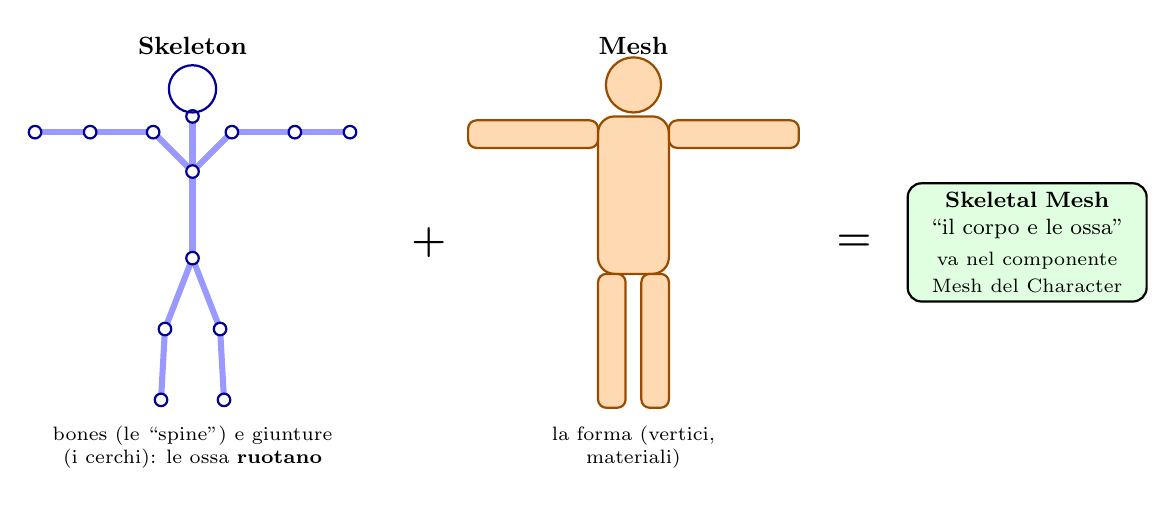
\begin{tikzpicture}[font=\footnotesize,
  ue8bone/.style={draw=blue!60!black, fill=blue!15, thick},
  ue8joint/.style={draw=blue!60!black, fill=white, thick, circle, inner sep=1.6pt}]
  % --- Skeleton (sinistra)
  \node[font=\small\bfseries] at (0,4.3) {Skeleton};
  \coordinate (pel) at (0,1.6); \coordinate (spi) at (0,2.7); \coordinate (nec) at (0,3.4);
  \coordinate (sl) at (-0.5,3.2); \coordinate (sr) at (0.5,3.2);
  \coordinate (el) at (-1.3,3.2); \coordinate (er) at (1.3,3.2);
  \coordinate (hl) at (-2.0,3.2); \coordinate (hr) at (2.0,3.2);
  \coordinate (kl) at (-0.35,0.7); \coordinate (kr) at (0.35,0.7);
  \coordinate (fl) at (-0.4,-0.2); \coordinate (fr) at (0.4,-0.2);
  \foreach \a/\b in {pel/spi, spi/nec, spi/sl, spi/sr, sl/el, sr/er, el/hl, er/hr,
                     pel/kl, pel/kr, kl/fl, kr/fr}
    \draw[ue8bone, line width=2.2pt, blue!40] (\a) -- (\b);
  \foreach \p in {pel, spi, nec, sl, sr, el, er, hl, hr, kl, kr, fl, fr}
    \node[ue8joint] at (\p) {};
  \draw[blue!60!black, thick] (0,3.75) circle (0.3);
  \node[font=\scriptsize, align=center] at (0,-0.8) {bones (le ``spine'') e
    giunture\\(i cerchi): le ossa \textbf{ruotano}};
  % --- piu'
  \node[font=\Large\bfseries] at (3.0,1.8) {+};
  % --- Mesh
  \begin{scope}[xshift=5.6cm]
    \node[font=\small\bfseries] at (0,4.3) {Mesh};
    \fill[orange!30, draw=orange!60!black, thick, rounded corners=6pt]
      (-0.45,1.4) rectangle (0.45,3.4);
    \fill[orange!30, draw=orange!60!black, thick] (0,3.8) circle (0.35);
    \fill[orange!30, draw=orange!60!black, thick, rounded corners=3pt]
      (-2.1,3.0) rectangle (-0.45,3.35);
    \fill[orange!30, draw=orange!60!black, thick, rounded corners=3pt]
      (0.45,3.0) rectangle (2.1,3.35);
    \fill[orange!30, draw=orange!60!black, thick, rounded corners=3pt]
      (-0.45,-0.3) rectangle (-0.1,1.4);
    \fill[orange!30, draw=orange!60!black, thick, rounded corners=3pt]
      (0.1,-0.3) rectangle (0.45,1.4);
    \node[font=\scriptsize, align=center] at (0,-0.8) {la forma (vertici,\\materiali)};
  \end{scope}
  % --- uguale
  \node[font=\Large\bfseries] at (8.4,1.8) {=};
  \node[draw, thick, rounded corners=5pt, fill=green!12, align=center, text width=2.8cm]
    at (10.6,1.8) {\textbf{Skeletal Mesh}\\``il corpo e le ossa''\\[2pt]
    \scriptsize va nel componente Mesh del Character};
\end{tikzpicture}
\caption{Skeletal Mesh e Skeleton secondo la lezione: due asset diversi. Lo Skeleton è
la gerarchia delle ossa, con le giunture; la Skeletal Mesh è la forma legata a quelle
ossa. Le animazioni sono rotazioni delle ossa, e sono legate allo Skeleton. Schema
ricostruito, non in scala.}
\label{ue8:fig:skeletal}
\end{figure}

\paragraph{Approfondimento: perché due asset.} Romero e Sewell (capitolo 17, ``Animation
Blueprints'') spiegano la separazione così: ``uno Skeleton è una gerarchia di ossa
interconnesse, usata per animare i vertici poligonali di una Skeletal Mesh''; e
``siccome l'animazione è fatta sullo Skeleton, può essere condivisa da molte Skeletal
Mesh che usano lo stesso Skeleton''. È il motivo per cui un gioco può avere decine di
personaggi diversi con un solo set di animazioni, e il motivo per cui, più avanti, le
animazioni del manichino di Unreal potranno essere \emph{ritargettate} sul cavaliere di
Mixamo, che ha uno scheletro simile ma non identico. Gli autori elencano anche i cinque
editor che si aprono dagli asset di animazione, con i bottoni in alto a destra già visti
dal docente: \emph{Skeleton Editor}, \emph{Skeletal Mesh Editor}, \emph{Animation
Editor}, \emph{Animation Blueprint Editor} e \emph{Physics Asset Editor}.

% ---------------------------------------------------------------------
\section{Le animazioni di Mixamo}
\label{ue8:sec:mixamoanim}

``Torniamo su Mixamo.'' L'importante è che nella viewport di Mixamo ci sia il proprio
personaggio, ``non un altro''; poi si passa alla categoria \textbf{Animations}. Servono
\textbf{tre animazioni} principali: \textbf{idle}, \textbf{walk} e \textbf{run}. ``La
idle, per chi non lo sapesse, sono le animazioni di stallo'': il personaggio ``sta fermo,
sta respirando'', il \emph{breathing}.

\paragraph{I controlli di Mixamo.} Sulla destra, per ogni animazione, ci sono alcuni
cursori; il docente li prova su animazioni diverse per farli vedere bene:
\begin{itemize}
  \item \textbf{Overdrive}: la velocità dell'animazione. ``Se aumento l'overdrive,
        questa animazione si velocizza sempre di più; se lo diminuisco, sarà
        lentissima'';
  \item \textbf{Character Arm-Space}: su alcuni modelli, la distanza delle braccia dal
        corpo, ``diventa sempre di più oppure diminuisce''. Attenzione al
        \emph{clipping}, le braccia che entrano nel corpo: ``infatti clippa
        malissimo''. Il docente suggerisce valori intorno a 50;
  \item \textbf{Trim}: ``tagliare l'animazione'', prenderne solo un pezzo. Ma ``viene
        fuori malissimo, perché non c'è il ritorno all'idle'': l'animazione tagliata non
        si chiude su sé stessa;
  \item \textbf{Mirror}: presente solo su alcune animazioni, ``semplicemente flippa
        l'animazione'', la \emph{specchia}. Il docente lo mostra con una Capoeira.
\end{itemize}

\paragraph{Root motion e in place.} Il punto più importante. Il docente apre un
\emph{Walking}: ``vedete che il character sta andando dritto, cioè sta percorrendo dello
spazio''. ``Questa tipologia di animazione viene chiamata \textbf{root motion}'': le
animazioni in root motion ``ereditano il movimento già nell'animazione''. L'esempio è
\emph{Dark Souls 3} (``qualcuno ha giocato Dark Souls 3? Perfetto''): alcune armi hanno
abilità speciali, le \emph{weapon art}, e in un video il docente cerca quella della
\emph{Holy Sword} (``questa non è in root motion, perché sta ferma''; ``eccola, questa
qua''): ``quando io la compio, mi sposto nello spazio già nell'animazione''. ``Non sono
io che gli do il movimento quando premo il tasto'': ``metto il piede in avanti, o faccio
l'affondo'', e il personaggio avanza perché lo fa l'animazione. Le animazioni in root
motion ``spesso sono usate per abilità'' di questo tipo.

``In questo caso, però, su Mixamo non dobbiamo avere un'animazione root motion'', perché
``erediteremmo un movimento che non ci interessa''. ``Noi, a livello del nostro gioco su
Unreal, vogliamo che l'animazione si compia, ma quella che si muove è la
\textbf{capsula}'': ``l'animazione segue la capsula''; ``c'è la mesh con l'animazione su
quella capsula, e di conseguenza si crea il movimento, o l'illusione del movimento''.
Quindi si spunta \textbf{In Place}: ``come potete vedere, adesso l'animazione è sul
posto''. ``Se non trovate una spunta In Place, consiglio di cambiare animazione: ce ne
sono tante'' (figura~\ref{ue8:fig:rootmotion}).

\begin{figure}[htbp]
\centering
\begin{tikzpicture}[font=\footnotesize,
  ue8cap/.style={draw=blue!60!black, thick, rounded corners=7pt, minimum width=0.7cm,
                 minimum height=1.6cm},
  ue8arr/.style={-{Stealth[length=2.4mm]}, very thick}]
  % root motion
  \node[font=\small\bfseries, anchor=west] at (-0.6,2.2) {Root motion};
  \node[ue8cap, fill=blue!8] at (0.3,0.9) {};
  \fill[orange!60] (0.3,1.5) circle (0.14);
  \draw[orange!60!black, very thick] (0.3,1.35) -- (0.3,0.75) -- (0.1,0.2);
  \draw[orange!60!black, very thick] (0.3,0.75) -- (0.5,0.2);
  \foreach \x/\o in {1.6/40, 2.9/60, 4.2/100} {
    \fill[orange!\o] (\x,1.5) circle (0.14);
    \draw[orange!\o!black, very thick] (\x,1.35) -- (\x,0.75) -- (\x-0.2,0.2);
    \draw[orange!\o!black, very thick] (\x,0.75) -- (\x+0.25,0.2);
  }
  \draw[ue8arr, orange!70!black] (0.6,-0.2) -- node[below, font=\scriptsize]
    {è l'animazione a spostare la mesh} (4.4,-0.2);
  \node[font=\scriptsize, align=left, text width=4.6cm, anchor=west] at (-0.6,-1.2)
    {la capsula resta indietro: mesh e collisione si separano. Utile per affondi e
    abilità (le weapon art di \emph{Dark Souls 3}), con Enable Root Motion};
  % in place
  \begin{scope}[xshift=7.4cm]
    \node[font=\small\bfseries, anchor=west] at (-0.6,2.2) {In place};
    \foreach \x/\o in {0.3/40, 1.6/60, 2.9/80, 4.2/100} {
      \node[ue8cap, fill=blue!8] at (\x,0.9) {};
      \fill[orange!\o] (\x,1.5) circle (0.14);
      \draw[orange!\o!black, very thick] (\x,1.35) -- (\x,0.75) -- (\x-0.2,0.2);
      \draw[orange!\o!black, very thick] (\x,0.75) -- (\x+0.25,0.2);
    }
    \draw[ue8arr, blue!60!black] (0.6,-0.2) -- node[below, font=\scriptsize]
      {è il Character Movement a spostare la capsula} (4.4,-0.2);
    \node[font=\scriptsize, align=left, text width=4.6cm, anchor=west] at (-0.6,-1.2)
      {l'animazione cammina sul posto, e la mesh segue la capsula: è quello che serve per
      idle, walk e run};
  \end{scope}
\end{tikzpicture}
\caption{Root motion e in place. In un'animazione root motion lo spostamento è dentro
l'animazione; in un'animazione in place il personaggio cammina sul posto, e a muoversi
nel mondo è la capsula del Character. Per la locomozione di base la lezione usa solo
animazioni in place. Schema ricostruito.}
\label{ue8:fig:rootmotion}
\end{figure}

\paragraph{Le impostazioni di download.} Al download Mixamo chiede alcune opzioni
(tabella~\ref{ue8:tab:mixamo}):
\begin{itemize}
  \item \textbf{Format}: \textbf{FBX Binary}, ``ci va bene così'';
  \item \textbf{Frames per Second}: \textbf{30}. ``Le animazioni devono essere allo
        stesso tipo di frame'': ``meglio sempre prenderle tutte quante allo stesso
        numero di frame'', ``perché se no avete dei problemi'', soprattutto ``nel
        \emph{blending}, cioè nel mixare'' due animazioni con frame rate diversi;
  \item \textbf{Skin}: \textbf{Without Skin}. ``La skin è se volete prendere
        l'animazione con il modello: non ci interessa, perché il modello ce l'abbiamo
        già'';
  \item \textbf{Keyframe Reduction}: \textbf{none}, ``non ci interessa'' ridurre i
        keyframe.
\end{itemize}
Il docente scrive in chat le tre animazioni da cercare, ``idle, walk e run/sprint'',
lasciando ``la libertà di scegliere quelle che volete'': ``importante che abbiate
un'animazione che respira, sta fermo, eccetera, una che cammina e una che fa lo
sprint''. Lui ha preso \emph{Idle}, \emph{Walking} e \emph{Slow Run}. ``Vi lascio 5, 10
minuti.''

\begin{table}[htbp]
\centering
\small
\begin{tabular}{@{}p{3.2cm}p{3.6cm}p{7.2cm}@{}}
\toprule
\textbf{Opzione} & \textbf{Valore} & \textbf{Perché} \\
\midrule
\multicolumn{3}{@{}l}{\emph{Personaggio}} \\
Format & FBX Binary & il formato che Unreal importa \\
Pose & T-Pose & la posa di riferimento del rig; togliere l'animazione applicata (la X) \\
\midrule
\multicolumn{3}{@{}l}{\emph{Animazioni (idle, walk, run)}} \\
Format & FBX Binary & come sopra \\
Skin & Without Skin & il modello c'è già: serve solo il movimento delle ossa \\
Frames per Second & 30 & tutte allo stesso frame rate, per non avere problemi nel
blending \\
Keyframe Reduction & none & nessuna riduzione dei keyframe \\
In Place & spuntato & niente root motion: a muoversi è la capsula \\
Overdrive, Arm-Space, Trim, Mirror & a piacere & velocità, distanza delle braccia
(attenzione al clipping), taglio, specchio \\
\bottomrule
\end{tabular}
\caption{Le impostazioni di download di Mixamo indicate a lezione.}
\label{ue8:tab:mixamo}
\end{table}

\paragraph{Approfondimento: Mixamo e Unreal.} Mixamo è un servizio gratuito di Adobe, a
cui si accede con un account Adobe; personaggi e animazioni si possono usare anche in
progetti commerciali. Il suo rig ha una gerarchia simile a quella del manichino di
Unreal (Manny e Quinn), ma i nomi delle ossa sono diversi (le ossa di Mixamo hanno il
prefisso \emph{mixamorig:}), e manca un osso \emph{root} alla base, sotto il bacino.
Per questo le animazioni di Mixamo in root motion non funzionano bene in Unreal senza
correzioni: lo spostamento è registrato sull'osso del bacino (\emph{Hips}) invece che su
un root. Con le animazioni \emph{In Place}, come quelle della lezione, il problema non si
pone. La mancanza dell'osso root e i nomi diversi sono anche il motivo per cui, per usare
sul cavaliere le animazioni del manichino (il salto, la caduta), servirà il
\textbf{retargeting} annunciato dal docente, con gli asset \emph{IK Rig} e \emph{IK
Retargeter} di Unreal Engine 5.

% ---------------------------------------------------------------------
\section{Importare le animazioni sullo scheletro}
\label{ue8:sec:importanim}

Dopo i minuti di scelta (``ci siete tutti, ragazzi? Sì, perfetto'') si importano le
animazioni. I file scaricati hanno il nome dell'animazione (``slow run, walking,
eccetera''); ``l'importante è che ci sia FBX sopra''. Al docente una delle due versioni
di Walking era rotta, e usa \emph{Walking 1}. ``Consiglio: fate meglio una cartella'':
\textbf{Animation}. ``Fatela una per una, vi consiglio.''

\paragraph{Lo scheletro obbligatorio.} La finestra di import è ``praticamente la stessa
schermata'', ``ma differenza sostanziale'': in basso, \textbf{Import} è grigio, non si
può premere. ``Per l'animazione in particolare gli serve uno scheletro a cui adattare
l'animazione.'' Nella sezione \textbf{Common} c'è il campo \textbf{Skeleton}: si apre la
tendina, in cui compaiono ``tutti gli scheletri'', compreso quello del manichino ``che
usiamo per Unreal'', e si sceglie \emph{il proprio}, quello creato dall'import del
personaggio. ``A questo punto, Import vi diventa blu.'' Nella stessa finestra il docente
indica anche la spunta sull'import della sola animazione (nella trascrizione: ``fate sì
che Import Only Animation sia ok''); la frase che segue è confusa.

\paragraph{Targettare.} ``Ecco a voi che si è creata un'animazione.'' ``Il file di per sé
è a parte, però lui ha \textbf{targettato}'' (``prendete questo termine'') ``la nostra
animazione su quello scheletro in particolare''. Un'animazione appartiene a uno
scheletro, e si può usare solo con le mesh di quello scheletro.

\paragraph{Approfondimento: le opzioni di import di un'animazione.} Nella finestra FBX
di Unreal Engine 5, quando il campo \emph{Skeleton} è impostato e la spunta
\emph{Import Mesh} è tolta, Unreal importa \emph{solo} le animazioni contenute nel file,
senza creare un'altra Skeletal Mesh e un altro scheletro; con \emph{Import Animations}
attivo, ogni animazione diventa un asset \textbf{Animation Sequence}. È il caso dei file
di Mixamo scaricati \emph{Without Skin}, che contengono solo le ossa animate. Se invece
si lascia vuoto il campo Skeleton su un file con la mesh, Unreal crea uno scheletro nuovo
a ogni import: è facile ritrovarsi con due scheletri quasi identici (``mi sa che ci sono
due ragazzi che hanno importato due'' scheletri, osserva il docente sulla sua tendina) e
con animazioni non compatibili fra loro.

% ---------------------------------------------------------------------
\section{L'editor dell'animazione}
\label{ue8:sec:animeditor}

Con un doppio clic sull'animazione si apre l'\textbf{Animation Editor}, ``che vi permette
di visualizzare tutte le particolarità della nostra animazione''.

\paragraph{I controlli.} In basso c'è il pannello di controllo: andare al primo o
all'ultimo frame (\emph{To Front}, \emph{To End}), al frame precedente o successivo
(``frame per frame per frame''). ``Le animazioni sono costituite da frame'': questa ne ha
\textbf{30}. Con \textbf{spazio}, o con il pulsante, \emph{Play} e \emph{Pause}.

\paragraph{Asset Details.} Sul lato dell'editor c'è il pannello \textbf{Asset Details}
(``se non vedete una finestra, la potete trovare su Window $\rightarrow$ Asset Details'',
``o Finestra $\rightarrow$ Dettagli dell'asset, suppongo, in italiano''). Ci sono molti
dati ``che nessuno andrebbe a vedere''; le cose principali:
\begin{itemize}
  \item \textbf{Loop}: ``se questa animazione la vogliamo che vada in loop'': ``quando
        finisce, ricomincia'';
  \item \textbf{Rate Scale}: a 1 è la velocità normale; ``se metto 1,5 l'animazione è
        più veloce''; a 2 ancora di più; ``40, diventa un casino''. ``È un po' come
        l'overdrive che abbiamo visto'' su Mixamo;
  \item \textbf{Root Motion}: la spunta \emph{Enable Root Motion} non è attiva, ``va
        bene così'', perché l'animazione è in place.
\end{itemize}
Lo stesso per le altre due animazioni: Idle, Slow Run (``vi chiederà sempre lo
scheletro''). ``Se aprite le vostre animazioni, sono giuste, sono davanti a voi?'' Alla
fine: ``dovreste avere tutte e tre le nostre belle animazioni''.

% ---------------------------------------------------------------------
\section{L'Animation Blueprint}
\label{ue8:sec:abp}

``La domanda sorge spontanea: come facciamo a metterle su un character?'' Con
l'\textbf{Animation Blueprint}.

\paragraph{La creazione.} Nella cartella del personaggio (il docente l'ha chiamata
\textbf{Characters}) si crea una cartella \textbf{Blueprint}. Poi tasto destro,
\textbf{Animation $\rightarrow$ Animation Blueprint}. La finestra chiede ``di quale
scheletro'': si sceglie il proprio (il docente, ``il mio paladino''), \textbf{Create}, e il
nome: \textbf{ABP\_Knight}, con il prefisso ABP per \emph{Animation Blueprint} (``io ho
chiamato Knight, però voi chiamatelo Ciccio Baciccio''). A uno studente che non ha
capito, il docente ripete: ``Animation, Animation Blueprint; vi chiederà lo scheletro;
selezionate lo scheletro vostro''. L'Animation Blueprint ``sarà la logica, quindi la
parte di programmazione'' delle animazioni ``del nostro bellissimo nuovo character''.

\paragraph{L'editor.} ``L'Animation Blueprint è abbastanza pieno di roba'', ``ci si può
confondere facilmente''. Le parti:
\begin{itemize}
  \item a sinistra, la \textbf{preview}, con il cavaliere in T-pose: ``e va benissimo,
        perché è la sua forma base'';
  \item l'\textbf{AnimGraph}, con il blocco \textbf{Output Pose}: ``tutti i calcoli che
        andremo a fare di animazioni'' si collegano a lui, ``e questo blocco ci dice:
        guarda, esce fuori questa roba'';
  \item l'\textbf{Event Graph}, ``come ce l'abbiamo in un classico Blueprint'', dove si
        possono ``creare e prendere variabili, modificare cose''.
\end{itemize}
``Esistono due ambienti particolari'': nel primo, l'AnimGraph, ``si ragiona per quanto
riguarda le animazioni''; nel secondo, l'Event Graph, ``a livello di programmazione''.

\paragraph{I due dati che servono.} Nell'Event Graph si devono ricavare due cose dal
personaggio:
\begin{enumerate}
  \item la \textbf{velocità}, ``perché vogliamo che la nostra animazione di camminata e
        di corsa, o di idle, sia relativa alla velocità che abbiamo al momento col
        character''. ``C'è una comunicazione tra i dati di gioco, quindi il movimento, e
        le animazioni'': ``dato un certo valore di velocità, cambia l'animazione'';
  \item se il personaggio \textbf{sta cadendo} o no, ``in modo da dire: guarda, sto
        saltando, sto iniziando a cadere; fammi un'animazione di salto, e fammi il loop
        del \emph{falling}''.
\end{enumerate}
Le animazioni di salto e caduta ``non le abbiamo importate'': ``le andremo a
ritargettare in seguito'', perché ``Unreal ci mette a disposizione la possibilità di
ritargettare delle animazioni'', ``ma non lo vedremo adesso''.

\paragraph{Event Blueprint Initialize Animation.} Il primo nodo è \textbf{Event Blueprint
Initialize Animation}: ``dice: quando l'animazione inizia''. ``Come abbiamo visto, gli
eventi come il Begin Play vengono fatti quando viene inizializzato tutto'': questo ``è il
Begin Play, ma per le animazioni''. (A questo punto Unreal si blocca di nuovo:
``è crashato Unreal; direi che oggi è proprio una gran roba''. ``Mi sa che mi tocca
svuotare un po' di memoria.'' Liberata la memoria, si riparte.)

\paragraph{Try Get Pawn Owner.} Dall'evento si chiama \textbf{Try Get Pawn Owner}.
``Questo blocco ci permette di comunicare con il nostro Pawn'', ``il nostro player''.
``Immaginatevi due ambienti separati'': nel Gameplay Framework ``il Pawn è quello che
controlla il character'', mentre l'animazione ``è subordinata al Pawn''. ``Quindi andiamo
a dire: ehi, provami a prendere l'owner, cioè il pawn owner.'' Poi ``andiamo a fare un
cast: abbiamo detto BP\_Knight\ldots{} Ah, giusto, ragazzi. Abbiamo scordato una cosa.
Dobbiamo creare effettivamente il nostro character.''

% ---------------------------------------------------------------------
\section{Il nuovo Character: BP\_Knight1}
\label{ue8:sec:character}

``Dobbiamo comunicare con il nostro character, per dire: guarda, mi servono questi dati
del movimento.'' Nella cartella Blueprint del personaggio: \textbf{Blueprint Class}, e
``attenzione'': come genitore si sceglie \textbf{Character}. Il nome:
\textbf{BP\_Knight1}.

\paragraph{I componenti del Character.} ``I character, a differenza degli actor, sono
costituiti di base da'':
\begin{itemize}
  \item un \textbf{Capsule Component}, la capsula;
  \item una \textbf{freccia} (\emph{Arrow}), ``per far capire qual è il forward vector
        della capsula'';
  \item la \textbf{Mesh}, una Skeletal Mesh;
  \item il \textbf{Character Movement}, ``il componente che definisce il movimento del
        character''. Nei suoi Details, in \emph{General Settings}, ci sono la
        \textbf{Gravity Scale}, la \textbf{Max Acceleration}, la \textbf{Braking
        Friction}. ``Come abbiamo detto, dobbiamo interfacciare le animazioni con i
        valori del movimento'', e quei valori stanno qui.
\end{itemize}

\paragraph{La Skeletal Mesh.} Nella Mesh si assegna la Skeletal Mesh del cavaliere (``devo
ricordarmi l'indirizzo''; ``no, non è questo, è questo qua''). Il personaggio ``è apparso
in modo abbastanza scorretto'', fuori posto rispetto alla capsula e girato male: ``basta
riposizionarlo''. ``Consiglio di fare lo \textbf{snapping}'': si abbassa la mesh in modo
che i piedi tocchino il fondo della capsula, e la si ruota ``in direzione della capsule'',
cioè con la faccia nella direzione della freccia (per i personaggi di Mixamo
serve di solito una rotazione di $-$90 gradi sulla Z; il valore esatto la trascrizione
non lo dice). ``Eccovi che abbiamo creato il nostro primo character.
Questa è la T-pose, meraviglioso.''

\paragraph{L'Anim Class.} ``Ma in questo caso non ha ancora animazioni.'' ``Come facciamo
a dire: guarda, devi usare proprio questa Animation Blueprint?'' Nella \textbf{Mesh}, alla
voce \textbf{Anim Class}, la tendina mostra tutti gli Animation Blueprint compatibili:
si sceglie \textbf{ABP\_Knight1} (il nome dell'asset del docente). ``Non è cambiato
niente, ma l'abbiamo messo in comunicazione'': quando l'Animation Blueprint avrà delle
animazioni, ``questo qua si aggiornerà''. La relazione è a due vie: il Character dice
quale Animation Blueprint usare (Anim Class), e l'Animation Blueprint chiede al suo
proprietario i dati (Try Get Pawn Owner).

% ---------------------------------------------------------------------
\section{Initialize: il cast e le referenze}
\label{ue8:sec:initialize}

Tornati nell'Animation Blueprint, il grafo dell'inizializzazione si completa
(figura~\ref{ue8:fig:abpgraph}, in alto):
\begin{enumerate}
  \item \textbf{Event Blueprint Initialize Animation};
  \item \textbf{Try Get Pawn Owner} $\rightarrow$ \textbf{Cast To BP\_Knight1}
        (``castate al vostro character, come l'avete chiamato'');
  \item dal pin As BP Knight1, \textbf{Promote to Variable}: una variabile referenza
        \textbf{BP\_Knight1}. ``Andiamo a creare una referenza del character, in modo
        tale che sia più semplice'': ``ogni volta che dovremmo prendere una cosa del
        character, dovremmo, se no, fare sempre Cast To BP\_Knight'', ed ``appesantisce
        castare sempre un qualcosa. Quindi lo facciamo all'inizio'';
  \item dalla referenza, \textbf{Get Character Movement}, ``per essere anche un po' più
        esaustivi'', e anche questo \textbf{Promote to Variable}: una variabile
        \textbf{MovementComponent}. ``Abbiamo creato già due variabili che ci faranno
        comodo in seguito.''
\end{enumerate}

\paragraph{Approfondimento: lo stesso grafo del modello Third Person.} Il grafo costruito
dal docente ricalca quasi nodo per nodo l'Animation Blueprint del manichino di Unreal
Engine 5 (\emph{ABP\_Manny}, nel modello Third Person): sull'Initialize, Try Get Pawn
Owner, Cast To Character, Set \emph{Character}, Get Character Movement, Set
\emph{MovementComponent}; sull'Update, controllo di validità, poi Set \emph{Velocity},
Set \emph{GroundSpeed} (Vector Length XY), Set \emph{ShouldMove} e Set \emph{IsFalling}.
La differenza è il cast: il modello fa Cast To \emph{Character}, la classe generica,
così che lo stesso Animation Blueprint funzioni con qualsiasi personaggio basato su
Character; la lezione fa Cast To BP\_Knight1, che dà accesso anche alle variabili
aggiunte nel cavaliere (utile, per esempio, per uno sprint), ma lega l'ABP a quella
classe.

% ---------------------------------------------------------------------
\section{Update: la velocità e la caduta}
\label{ue8:sec:update}

\paragraph{Event Blueprint Update Animation.} ``Questo evento avviene quasi come il Tick,
a ogni frame.'' ``Quando un'animazione si aggiorna, qualsiasi micro movimento è un
Update'': ``se abbiamo un idle, comunque è un'animazione; un walk, comunque è
un'animazione; e il run, comunque è un'animazione'', ``quindi sarà sempre attivo''. ``È
per questo che non facciamo il cast qui'': ``se no farebbe ogni volta, ogni frame,
sempre molto pesante''.

\paragraph{Il Validated Get.} ``Dobbiamo vedere se questo character è valido.'' ``Vi
ricordate gli Is Valid? Se in una variabile c'è qualcosa dentro o non c'è.'' C'è ``una
cosa molto interessante'': si trascina nel grafo un \textbf{Get} della variabile
BP\_Knight1, tasto destro, \textbf{Convert to Validated Get}. Il Get ``normale'' prende la
variabile e basta; il Validated Get ``prende la variabile, e mette anche la
particolarità: se lo prendo ed è valido faccio questo, se non è valido faccio
quest'altro''. Ha un ingresso di esecuzione e due uscite, \textbf{Is Valid} e \textbf{Is
Not Valid}: un Get e un Is Valid in un nodo solo. Sull'uscita Is Valid il docente mette
una \textbf{Sequence} (``un Is Valid, Sequence'') per eseguire in ordine le operazioni
che seguono.

\paragraph{GroundSpeed.} ``Fondamentalmente andiamo a prendere il Movement Component'',
la variabile creata nell'Initialize, e da lì \textbf{Get Velocity}: ``la velocità attuale,
a ogni frame, del character movement''. È un vettore; ``ci interessa solamente il
movimento'' sul piano, ``non ci interessa se salta o meno'', ``quello ci interesserà in
altro modo''. Quindi il nodo \textbf{Vector Length XY}: ``la lunghezza del vettore
solamente sugli assi X e Y'', ``se l'asse X è avanti e dietro e l'asse Y è destra e
sinistra''. Il risultato è un \textbf{float}, e diventa, con \textbf{Promote to
Variable}, \textbf{GroundSpeed}: ``una variabile che rappresenta la nostra velocità
attuale''.

\paragraph{IsFalling.} ``Molto importante per sapere quando saltiamo o quando stiamo
cadendo'': dal Movement Component, il nodo \textbf{Is Falling}. ``Ce ne sono due'': uno è
quello del \emph{Nav Movement}; quello giusto ``deve essere blu all'inizio e rosso alla
fine'', cioè con l'ingresso target blu (il Character Movement) e l'uscita rossa (una
booleana). Il valore va in una variabile, \textbf{IsFalling}, aggiornata a ogni frame,
``in modo tale da sapere che movimento fargli fare'' nel ``giro di animazioni''.

\paragraph{Velocity.} ``Per il futuro, per altre cose che ci serviranno'', anche il
vettore della velocità si promuove a variabile: \textbf{Velocity}, ``così almeno ci sono
delle cose che vogliamo interfacciare con la velocità''. ``Adesso abbiamo tirato fuori la
nostra velocità attuale e il fatto se sta cadendo o meno.'' A uno studente il Get
Velocity non compare: è quello che si ottiene dal Movement Component, con il target
giallo e l'uscita gialla (un vettore); cercandolo in fondo alla lista, ``trovato''.

\begin{figure}[htbp]
\centering
\begin{tikzpicture}[font=\footnotesize,
  ue8node/.style={draw, thick, rounded corners=4pt, align=center, fill=gray!8,
                  minimum height=0.8cm, text width=2.0cm},
  ue8ev/.style={ue8node, fill=red!12},
  ue8pure/.style={ue8node, fill=green!10, rounded corners=8pt},
  ue8var/.style={ue8node, fill=blue!10, rounded corners=8pt},
  ue8exec/.style={-{Stealth[length=2.5mm]}, very thick, black!80},
  ue8data/.style={-{Stealth[length=2mm]}, thick, blue!60!black}]
  % Initialize
  \node[font=\small\bfseries, anchor=west] at (-1.2,1.3) {Inizializzazione (una volta)};
  \node[ue8ev, text width=2.3cm] (ini) at (0,0) {\textbf{Event Blueprint Initialize
    Animation}};
  \node[ue8node, fill=blue!10, text width=1.9cm] (cst) at (3.2,0) {\textbf{Cast To}\\
    BP\_Knight1};
  \node[ue8pure] (tgp) at (3.2,-1.6) {\textbf{Try Get}\\\textbf{Pawn Owner}};
  \node[ue8node, text width=2.0cm] (s1) at (6.2,0) {\textbf{Set}\\BP\_Knight1};
  \node[ue8node, text width=2.8cm] (s2) at (9.6,0) {\textbf{Set}\\Movement\-Component};
  \node[ue8pure, text width=2.6cm] (gcm) at (9.6,-1.6) {BP\_Knight1 $\rightarrow$\\
    \textbf{Get Character Movement}};
  \draw[ue8exec] (ini) -- (cst);
  \draw[ue8data] (tgp) -- node[right, font=\scriptsize]{Object} (cst);
  \draw[ue8exec] (cst) -- (s1);
  \draw[ue8exec] (s1) -- (s2);
  \draw[ue8data] (gcm) -- (s2);
  % Update
  \node[font=\small\bfseries, anchor=west] at (-1.2,-3.1) {Aggiornamento (ogni frame)};
  \node[ue8ev, text width=2.3cm] (upd) at (0,-4.6) {\textbf{Event Blueprint Update
    Animation}};
  \node[ue8var, text width=2.0cm] (vg) at (3.3,-4.6) {\textbf{Validated Get}\\
    BP\_Knight1};
  \node[ue8node, text width=1.6cm] (seq) at (6.5,-4.6) {\textbf{Sequence}};
  \node[ue8node, text width=3.6cm, align=left] (sv) at (10.6,-3.4) {\textbf{Set
    Velocity} $\leftarrow$\\MovementComponent $\rightarrow$ Get Velocity};
  \node[ue8node, text width=3.6cm, align=left] (sg) at (10.6,-4.7) {\textbf{Set
    GroundSpeed} $\leftarrow$\\Vector Length XY (Velocity)};
  \node[ue8node, text width=3.6cm, align=left] (sf) at (10.6,-6.0) {\textbf{Set
    IsFalling} $\leftarrow$\\MovementComponent $\rightarrow$ Is Falling};
  \draw[ue8exec] (upd) -- (vg);
  \draw[ue8exec] (vg) -- node[above, font=\scriptsize]{Is Valid} (seq);
  \draw[ue8exec] (seq.east) -- ++(0.4,0) |- node[pos=0.75, above, font=\scriptsize]
    {Then 0} (sv.west);
  \draw[ue8exec] (seq.east) -- ++(0.4,0) |- node[pos=0.75, above, font=\scriptsize]
    {Then 1} (sg.west);
  \draw[ue8exec] (seq.east) -- ++(0.4,0) |- node[pos=0.75, above, font=\scriptsize]
    {Then 2} (sf.west);
\end{tikzpicture}
\caption{I due grafi dell'Event Graph di ABP\_Knight. In alto, una sola volta: si prende
il proprietario, lo si converte nel cavaliere e si salvano due referenze. In basso, a
ogni frame: se la referenza è valida, si aggiornano Velocity (vettore), GroundSpeed (la
sua lunghezza sul piano XY) e IsFalling (booleana). Accanto a ogni Set, il valore che riceve.
Schema ricostruito.}
\label{ue8:fig:abpgraph}
\end{figure}

\paragraph{Un registro di dati.} ``Questo graph funziona letteralmente come'' un
registro (la trascrizione dice ``registri di credito''): serve ``principalmente per
interfacciarsi con il nostro bellissimo character'', e ``ci serve per capire valori,
vedere cose'', ``parliamo di numeri per lo più''. Le animazioni vere si decidono altrove.

\paragraph{Approfondimento: perché l'AnimGraph non legge da solo.} Romero e Sewell
(capitolo 17) descrivono la stessa divisione dei compiti: ``usiamo l'EventGraph di un
Animation Blueprint per prendere i dati dal Pawn o dal Character che sta usando l'istanza
dell'Animation Blueprint, e per aggiornare le variabili dell'Animation Blueprint''; e
``l'AnimGraph può accedere solo alle variabili dell'Animation Blueprint''. Il loro esempio
è più semplice di quello della lezione: sull'Update un Is Valid sul Try Get Pawn Owner,
Get Velocity dal Pawn, \emph{VectorLength} (la lunghezza su tutti e tre gli assi) e Set
di una variabile \emph{Speed}. La scelta del docente, \textbf{Vector Length XY}, è più
precisa per la locomozione: con la lunghezza completa, un personaggio che cade dritto
verso il basso avrebbe una velocità alta e farebbe la corsa a mezz'aria. Gli autori
notano anche che \emph{Event Blueprint Update Animation} ha un parametro \emph{Delta Time
X}, il tempo trascorso dall'ultimo frame, utile per interpolare i valori.

% ---------------------------------------------------------------------
\section{L'AnimGraph, un'anteprima del Blend Space e il personaggio finito}
\label{ue8:sec:animgraph}

``Adesso, ragazzi, vi faccio una spiegazione teorica molto corta, perché capisco che siamo
agli ultimi dieci minuti, anzi sette.'' L'AnimGraph, ``differentemente, lavora per
esempio per \emph{state machine}''.

\paragraph{Un'animazione sull'Output Pose.} Il caso più semplice: nell'\textbf{Asset
Browser} dell'editor (``qua trovate tutte le animazioni che sono compatibili con questo
scheletro'') si prende un'animazione, per esempio \emph{Walking 1}, la si trascina
nell'AnimGraph e si collega ``l'omino'' del nodo all'omino dell'\textbf{Output Pose}. Non
è in loop, ma basta spuntare \textbf{Loop Animation} nei Details del nodo. Compile: nella
preview il cavaliere cammina. ``E possiamo vederlo anche nel nostro character'', perché
l'Anim Class ``ci ha permesso di dirgli: guarda, ehi, hai questo in eredità, hai questo
sotto di te, l'Animation Blueprint''. ``Ma, come potete capire, a noi serve molto di più
rispetto a mettere queste animazioni'' una alla volta.

\paragraph{Il Blend Space 1D.} ``Sicuramente la prossima volta andremo a vedere quelli
che sono chiamati \textbf{Blend Space}. Ve lo faccio vedere velocissimamente.'' Il
docente apre un \textbf{Blend Space 1D} (``una dimensione''), creato sullo scheletro del
cavaliere: un grafico con il personaggio che ``ci permette di mettere insieme varie
animazioni che \emph{blendano} tra di loro'', cioè ``che interpolano tra di loro''.
Nella preview, spostandosi sull'asse: idle, poi walking, poi sprint. ``In questo caso ci
sarà solamente un asse, che noi diremo che sarà la nostra \textbf{GroundSpeed}'', la
velocità ``che definisce il movimento'' (figura~\ref{ue8:fig:blendspace}). ``La prossima
volta vedremo di costruire questa tipologia di asset e collegare tutto quanto.''

\begin{figure}[htbp]
\centering
\begin{tikzpicture}[font=\footnotesize,
  ue8pt/.style={draw=black, fill=white, thick, diamond, inner sep=2.2pt}]
  \draw[-{Stealth[length=2.5mm]}, thick] (0,0) -- (11.2,0) node[right]{GroundSpeed};
  \foreach \x/\v in {0/0, 2.5/150, 5/300, 7.5/450, 10/600}
    \draw (\x,0.1) -- (\x,-0.1) node[below, font=\scriptsize]{\v};
  \node[ue8pt] (i) at (0,0) {}; \node[ue8pt] (w) at (2.5,0) {}; \node[ue8pt] (r) at
    (10,0) {};
  \node[above=6pt of i, font=\scriptsize\bfseries] {Idle};
  \node[above=6pt of w, font=\scriptsize\bfseries] {Walking};
  \node[above=6pt of r, font=\scriptsize\bfseries] {Run / Sprint};
  \fill[green!50!black] (6.25,0) circle (0.12);
  \draw[green!50!black, thick, ->] (6.25,0.9) -- (6.25,0.2);
  \node[green!40!black, font=\scriptsize, align=center] at (6.25,1.3) {valore attuale:
    50\% Walking + 50\% Run};
  \node[font=\scriptsize, align=center, text width=11cm] at (5.5,-1.0) {le animazioni
    sono campioni posti sull'asse; fra due campioni Unreal le mescola in proporzione
    alla distanza};
\end{tikzpicture}
\caption{Un Blend Space 1D come quello mostrato in anteprima: un solo asse, la
GroundSpeed calcolata nell'Event Graph, e tre animazioni poste su di esso. I valori
sull'asse sono un esempio, non quelli del docente. Schema ricostruito.}
\label{ue8:fig:blendspace}
\end{figure}

\paragraph{Il personaggio finito.} Per chiudere, il docente mostra dove arriveranno.
``Io posso cambiare il nostro character da qui'': nei \textbf{World Settings} del livello,
nella Game Mode, alla voce \textbf{Default Pawn Class}, sceglie BP\_Knight. In Play, il
cavaliere si muove con idle, camminata e corsa, e ``gli ho messo addirittura pure lo
sprint''. ``Il salto, questo è ritargettato'': è l'animazione classica di Unreal, portata
sullo scheletro di Mixamo. E la vecchia logica funziona con il nuovo personaggio:
``possiamo fare tutte le interazioni, e addirittura la nostra torretta ci segue''.
``Questo lo faremo la prossima volta'', ``perché ci vuole un pochino di continuità''.

\paragraph{Approfondimento: dalle animazioni singole alla State Machine.} Il capitolo 17
di Romero e Sewell mostra i passi successivi, quelli annunciati per la prossima lezione.
Un \textbf{Blend Space} è ``un tipo di asset che permette di mescolare animazioni in base
ai valori di uno o due parametri'': nel loro esempio del modello Third Person (UE4), il
Blend Space di locomozione pone \emph{Idle} a 0, \emph{Walk} a 93,75 e \emph{Run} a 375,
e con una velocità di circa 234 l'animazione risultante è metà camminata e metà corsa.
Trascinato nell'AnimGraph, il Blend Space diventa un nodo \emph{Blendspace Player} con un
ingresso per il parametro, a cui si collega la variabile della velocità; nell'\emph{Anim
Preview Editor} si può cambiare il valore e vedere il risultato senza andare in Play.
Poi la \textbf{State Machine}: un nodo dell'AnimGraph che organizza le animazioni in
\emph{stati} (per esempio \emph{Idle} e \emph{Moving}, e più avanti \emph{Jump} e
\emph{Fall}), collegati da \emph{transizioni} con regole booleane (per esempio
``GroundSpeed $>$ 3'' per passare da fermo a in movimento, o ``IsFalling'' per passare
al salto). È lì che la variabile IsFalling di oggi troverà il suo uso.

% ---------------------------------------------------------------------
\section{I materiali mancanti e la chiusura}
\label{ue8:sec:chiusura}

``Ci sono domande, ragazzi?'' Una studentessa: ``il mio personaggio non c'ha un
materiale, ha solo le texture''. ``Anche il mio non è importato'', aggiunge un altro.

\paragraph{Creare il materiale a mano.} La studentessa condivide lo schermo: il suo
personaggio di Mixamo è un'arciera (\emph{Erika Archer}, a giudicare dalla trascrizione).
``Se non hai un materiale, dovresti crearlo da zero'':
\begin{enumerate}
  \item tasto destro $\rightarrow$ \textbf{Material}, chiamato \textbf{M\_Archer};
  \item aperto il materiale in una finestra piccola, si trascinano dentro tutte le
        \textbf{texture} (``quelle con il label rosso''), che diventano nodi
        \textbf{Texture Sample};
  \item si legge bene il nome di ognuna: la \textbf{Diffuse} va nel \textbf{Base Color}
        (``acciaccala in Base Color''); la \textbf{Normal} va nel \textbf{Normal}.
\end{enumerate}
Leggendo i nomi, però, si scopre che le texture sono di due gruppi: una Diffuse dei
\emph{vestiti} e una della \emph{pelle} (e una delle ciglia, l'\emph{eyelash}). ``Ha due
materiali diversi, forse.'' ``Quindi mi sa che devi fare due materiali: uno per i
vestiti, e l'altro per la pelle'', per esempio \emph{M\_ArcherClothing}.

\paragraph{Gli slot dei materiali.} Per sapere dove va cosa, si apre la Skeletal Mesh:
nei Details, la sezione dei materiali mostra gli slot, con il \textbf{WorldGridMaterial}
(la griglia grigia di default) dove manca un materiale. Gli slot sono \emph{quattro}, non
due. Si mette il nuovo materiale nell'\textbf{Element 0} e si guarda ``dove te lo mette sul
corpo'': passando sopra uno slot, la parte corrispondente si illumina
(\emph{highlight}). Element 0 è il \emph{clothing}; il 2 e il 3 saranno la pelle, con un
altro materiale. ``Tanto, se non avete i materiali ma avete le texture, ragazzi, potete
farlo direttamente a mano.''

\paragraph{Le texture che non ci sono.} A un altro studente non sono state importate
nemmeno le texture. Il docente prova a riprodurre il problema: torna su Mixamo (``Mixamo
non mi risponde più, ottimo''), scarica lo stesso personaggio, \emph{The Boss}
(``use this character''; ``madonna mia''), in T-pose, e lo importa. Nella finestra di
import, nella sezione dei materiali, \textbf{Import Materials} e \textbf{Import
Textures} devono essere attivi (``fai sì che i materiali siano importati''); \emph{Import
Morph Targets} e simili ``non ci interessano''. ``A me importa tutto.'' ``Se c'hai
difficoltà, magari puoi semplicemente riprovare a fare l'import.'' Intanto Federico ha
risolto da solo, assegnando i materiali agli slot con l'highlight: ``allora vuol dire che
ti sei risolto la vita da solo. Perfetto.''

\paragraph{Approfondimento: Diffuse, Normal e gli altri canali.} Una \textbf{Diffuse} (o
\emph{Albedo}, o \emph{Base Color}) è il colore della superficie senza luci né ombre, e
va nel pin Base Color; una \textbf{Normal map}, riconoscibile dal colore azzurro-violetto,
simula i rilievi e va nel pin Normal (Unreal la riconosce all'import e imposta la
compressione \emph{Normalmap}). Se ci sono texture di \emph{Specular}, \emph{Roughness} o
\emph{Gloss}, vanno nei pin corrispondenti, ricordando che una Gloss è l'inverso di una
Roughness (serve un nodo \emph{1-x}, \emph{OneMinus}). Per le ciglia e i capelli, fatti
di piani con trasparenze, il materiale va impostato con \emph{Blend Mode} \emph{Masked}
e l'alfa della texture collegata all'\emph{Opacity Mask}: altrimenti le ciglia appaiono
come rettangoli pieni. Sono gli stessi nodi visti nella terza lezione, dedicata a
texture e materiali.

\paragraph{La chiusura.} ``Altri problemi? Se no, ci sentiamo la prossima volta.''
``Se dovete dichiarare qualcosa, non alla dogana, spero, ci sentiamo su Discord'':
``mandatemi quello che volete, se provate cose''. A Filippo: ``poi magari ti guardo un po'
quelle cosette che abbiamo visto prima''. ``Allora, ragazzi, buona cena, buona serata.
Ci vediamo giovedì. Ciao, ciao.''

\begin{table}[htbp]
\centering
\small
\begin{tabular}{@{}p{5.4cm}p{8.6cm}@{}}
\toprule
\textbf{Sintomo} & \textbf{Causa e rimedio} \\
\midrule
Una variabile ``non si muove'' & creata di nuovo e rimasta al default (0): controllare i
valori; variabili con nomi chiari \\
Errore sull'Audio Component ``non valido'' (Set Pitch Multiplier), solo arrivando in
fondo & caso rimasto aperto; ipotesi: lo Stop distrugge il suono (Auto Destroy) e la
variabile resta a puntare al vuoto. Is Valid, o Auto Destroy disattivato, o reset del Do
Once \\
L'ascensore va sempre più giù e non risale & attivazioni ripetute: booleana Activated
(Branch sul False all'inizio di Activation, false sul Begin Overlap) \\
Il progetto non si apre (si apre solo Unreal) & probabile chiavetta USB staccata male:
rimuoverla in sicurezza; usare un sistema di versione (Git) \\
Il personaggio si ferma un istante sul collezionabile & doppia collisione: mesh in
NoCollision, resta la Sphere Collision \\
On Component Begin Overlap non compare & è selezionata la mesh e non la Collision \\
Get Collectables non compare da Get Game Instance & manca il Cast To GI\_Platform: la
referenza è generica \\
Il cast non funziona & Get Game Instance non collegato all'Object del cast \\
``Non eredita da istanza di gioco''; la classe non compare nei Project Settings & la
Game Instance è stata creata con un altro genitore: ricrearla da GameInstance, sceglierla
in Game Instance Class, rifare variabile e cast \\
Il collezionabile conta ma l'esecuzione si ferma & il filo di esecuzione non passa per
il cast \\
Open Level non carica il livello & nome scritto male: è case sensitive. Copiarlo con F2,
Ctrl+C, Ctrl+V \\
Le palline raccolte riappaiono & normale: il livello viene ricaricato. Salvare lo stato
nella Game Instance (esercizio futuro) \\
Mettere a terra un componente nel Blueprint & nessuna scorciatoia (End vale solo nel
livello): regolare la Z a mano \\
Errore su Set Play Rate all'uscita dal Play & una vecchia referenza alla timeline con lo
stesso nome: eliminarla e usare quella giusta \\
Unreal si chiude durante l'import & memoria video esaurita: liberare memoria e spazio su
disco, reimportare \\
Il personaggio importato è ruotato & Offset Rotation non a zero: controllare Offset
Translation e Rotation all'import \\
Import grigio per un'animazione & manca lo Skeleton: sceglierlo in Common
$\rightarrow$ Skeleton \\
L'animazione sposta il personaggio da sola & è in root motion: riscaricarla da Mixamo
con In Place \\
Get Velocity non compare & cercarlo dal Movement Component (target e uscita gialli) \\
Il personaggio di Mixamo è grigio, senza materiale & creare i materiali a mano (Diffuse
in Base Color, Normal in Normal) e assegnarli agli slot; o reimportare con Import
Materials e Import Textures \\
\bottomrule
\end{tabular}
\caption{I problemi incontrati durante la lezione, con la causa e il rimedio.}
\label{ue8:tab:errori}
\end{table}

\begin{table}[htbp]
\centering
\small
\begin{tabular}{@{}p{4.6cm}p{9.4cm}@{}}
\toprule
\textbf{Nodo, asset o impostazione} & \textbf{Che cosa fa} \\
\midrule
Game Instance (Blueprint Class) & l'oggetto che vive per tutto il gioco; contiene dati
globali \\
Project Settings $\rightarrow$ Maps \& Modes $\rightarrow$ Game Instance Class & sceglie
la Game Instance del progetto \\
Get Game Instance & restituisce la Game Instance, come referenza generica \\
Cast To (classe) & converte una referenza nel tipo specifico; Cast Failed se non lo è \\
Increment Int (++) / Decrement Int ($--$) & aggiunge o toglie 1 a una variabile intera \\
Collision Presets: NoCollision & toglie ogni collisione a un componente \\
Sphere Collision, Sphere Radius & volume sferico e il suo raggio \\
Destroy Actor & distrugge l'actor \\
Evento Key (E) & scatta alla pressione di un tasto (Pressed, Released) \\
Text Render & un testo nel mondo 3D \\
Hidden in Game & nasconde un componente in gioco; tolto, la box si vede \\
Open Level (by Name) & carica un livello dal nome (case sensitive) \\
File $\rightarrow$ New Level (Basic) & un livello con cielo, luce e pavimento \\
Skeletal Mesh / Skeleton / Physics Asset & la mesh con le ossa; la gerarchia delle ossa;
i corpi fisici \\
Offset Translation / Rotation (import) & posizione e rotazione dell'asset rispetto al
pivot \\
Animation Sequence: Loop, Rate Scale, Enable Root Motion & ripetizione, velocità,
movimento dentro l'animazione \\
Animation Blueprint (ABP) & la logica delle animazioni di uno scheletro: Event Graph e
AnimGraph \\
Anim Class (Mesh del Character) & l'Animation Blueprint usato dalla mesh \\
Character (Capsule, Arrow, Mesh, Character Movement) & il Pawn che cammina, salta,
nuota, vola \\
Event Blueprint Initialize Animation & il ``Begin Play'' dell'Animation Blueprint \\
Try Get Pawn Owner & il Pawn che usa l'Animation Blueprint \\
Event Blueprint Update Animation & scatta a ogni aggiornamento dell'animazione, come il
Tick \\
Convert to Validated Get & un Get con le uscite Is Valid e Is Not Valid \\
Sequence & esegue più uscite in ordine \\
Get Velocity / Vector Length XY & la velocità; la sua lunghezza sul piano \\
Is Falling (Character Movement) & vero se il personaggio è in aria \\
Output Pose (AnimGraph) & la posa finale applicata alla mesh \\
Blend Space 1D & mescola animazioni lungo un asse (GroundSpeed) \\
World Settings $\rightarrow$ Default Pawn Class & il personaggio del giocatore in quel
livello \\
\bottomrule
\end{tabular}
\caption{I nodi, gli asset e le impostazioni dell'ottava lezione.}
\label{ue8:tab:nodi}
\end{table}

% ---------------------------------------------------------------------
\section*{Punti chiave del capitolo}
\addcontentsline{toc}{section}{Punti chiave del capitolo}

\begin{itemize}
  \item Il \textbf{Gameplay Framework} è la gerarchia delle entità che Unreal crea mentre
        il gioco gira: \textbf{Game Instance} (per tutta la durata del gioco), livello,
        \textbf{Game Mode} (le regole), \textbf{Game State} e \textbf{Player State} (lo
        stato, condiviso in rete), \textbf{Player Controller} (il ``cervello'' non
        fisico), \textbf{Pawn} e \textbf{Character} (il ``corpo''), e infine l'input.
  \item \textbf{Pubblica non vuol dire globale}: le variabili degli actor muoiono con il
        livello. Per conservare dati fra i livelli si usa la \textbf{Game Instance},
        creata come Blueprint Class da GameInstance e scelta in \textbf{Project Settings
        $\rightarrow$ Maps \& Modes $\rightarrow$ Game Instance Class}. Non va
        appesantita, perché resta in memoria per tutta la partita.
  \item \textbf{Get Game Instance} restituisce una referenza generica, ``la scocca'':
        per leggere le nostre variabili serve il \textbf{Cast To} della nostra classe,
        ``l'abito giusto'' per entrare alla festa. Cast Failed non è un errore, è una
        risposta.
  \item Un \textbf{collezionabile}: Sphere Collision, mesh in \textbf{NoCollision} (niente
        doppia collisione), controllo sul player, \textbf{Increment Int} sulla variabile
        della Game Instance, \textbf{Destroy Actor}.
  \item Un volume che cambia livello: \textbf{Open Level (by Name)} con il nome promosso
        a variabile pubblica. I nomi sono \textbf{case sensitive}: copiarli con F2 e
        Ctrl+C. I livelli nuovi da \textbf{File $\rightarrow$ New Level $\rightarrow$
        Basic}, salvati subito con Ctrl+S.
  \item Una booleana \textbf{Activated} con un Branch fa da cancello: l'ascensore
        ignora le attivazioni ripetute finché il player non lo fa risalire.
  \item Una \textbf{Skeletal Mesh} è ``il corpo e le ossa''; lo \textbf{Skeleton} è un
        asset separato, a cui sono legate le animazioni. Le ossa si \textbf{ruotano},
        non si spostano.
  \item Da \textbf{Mixamo}: personaggio in \textbf{T-pose}, \textbf{FBX Binary};
        animazioni idle, walk e run \textbf{In Place} (non root motion: a muoversi è la
        capsula), \textbf{Without Skin}, \textbf{30 fps} per tutte, nessuna riduzione dei
        keyframe. All'import si controllano gli \textbf{Offset}; le animazioni si
        importano scegliendo lo \textbf{Skeleton}.
  \item L'\textbf{Animation Blueprint} ha due grafi: l'\textbf{Event Graph} raccoglie i
        dati dal personaggio, l'\textbf{Anim\-Graph} decide la posa (\textbf{Output
        Pose}). Il Character lo usa tramite l'\textbf{Anim Class} della Mesh.
  \item Nell'\textbf{Initialize}: Try Get Pawn Owner, Cast To del personaggio, e le
        referenze salvate in variabili (il cast una volta sola). Nell'\textbf{Update},
        che gira a ogni frame: \textbf{Validated Get}, poi \textbf{GroundSpeed} (Vector
        Length XY della Get Velocity), \textbf{IsFalling} e \textbf{Velocity}.
  \item Prossimi passi: il \textbf{Blend Space 1D} sulla GroundSpeed, la State Machine,
        il \textbf{retargeting} del salto, e il personaggio impostato come
        \textbf{Default Pawn Class}.
\end{itemize}
